% !TEX TS-program = XeLaTeX
%%%%%%%%%%%%%%%%%%%%%%%%%%%%%%%%%%%%%%%%%
% Classicthesis Typographic Thesis
% LaTeX Template
% Version 1.4 (1/1/16)
%
% This template has been downloaded from:
% http://www.LaTeXTemplates.com
%
% Original author:
% André Miede (http://www.miede.de) with commenting modifications by:
% Vel (vel@LaTeXTemplates.com)
%
% License:
% GNU General Public License (v2)
%
% General Tips:
% 1) Make sure to edit the classicthesis-config.file
% 2) New enumeration (A., B., C., etc in small caps): \begin{aenumerate} \end{aenumerate}
% 3) For margin notes: \marginpar or \graffito{}
% 4) Do not use bold fonts in this style, it is designed around them
% 5) Use tables as in the examples
% 6) See classicthesis-preamble.sty for useful commands
%
%%%%%%%%%%%%%%%%%%%%%%%%%%%%%%%%%%%%%%%%%

%----------------------------------------------------------------------------------------
%	PACKAGES AND OTHER DOCUMENT CONFIGURATIONS
%----------------------------------------------------------------------------------------

\documentclass[
                %twoside,openright, BCOR=5mm,
                titlepage,numbers=noenddot,headinclude,%1headlines,
	 	footinclude=true,cleardoublepage=empty,
		dottedtoc, % Make page numbers in the table of contents flushed right with dots leading to them
                paper=a4,fontsize=12pt, % Binding correction, paper type and font size
		american, % Languages, change this to your language(s)
		]{scrreprt} 
                
% Includes the file which contains all the document configurations and packages - make sure to edit this file
%%%%%%%%%%%%%%%%%%%%%%%%%%%%%%%%%%%%%%%%%
% Classicthesis Typographic Thesis
% Configuration File
%
% This file has been downloaded from:
% http://www.LaTeXTemplates.com
%
% Original author:
% André Miede (http://www.miede.de) with extensive commenting changes by:
% Vel (vel@LaTeXTemplates.com)
%
% License:
% GNU General Public License (v2)
%
% Important note:
% The main lines to change in this file are in the DOCUMENT VARIABLES
% section, the rest of the file is for advanced configuration.
%
%%%%%%%%%%%%%%%%%%%%%%%%%%%%%%%%%%%%%%%%%

%----------------------------------------------------------------------------------------
%	CHARACTER ENCODING
%----------------------------------------------------------------------------------------

% Disabled because xelatex
%\usepackage{inputenc}

%----------------------------------------------------------------------------------------
%	DOCUMENT VARIABLES
%	Fill in the lines below to enter your information into the thesis template
%	Each of the commands can be cited anywhere in the thesis
%----------------------------------------------------------------------------------------

%\PassOptionsToPackage{eulerchapternumbers,listings,subfig,beramono,parts,manychapters}{classicthesis}
\PassOptionsToPackage{eulerchapternumbers,listings,subfig,beramono,parts,manychapters}{classicthesis}
% Available options: drafting parts nochapters linedheaders eulerchapternumbers beramono eulermath pdfspacing minionprospacing tocaligned dottedtoc manychapters listings floatperchapter subfig
% Might want to turn of xelatex and re-enable pdfspacing

\newcommand{\myTitle}{A Search for Lightly Ionizing Particles in the LUX Detector and R\&D For Future Experiments\xspace}
\newcommand{\mySubtitle}{Subtitle\xspace}
\newcommand{\myDegree}{Doctor of Philosophy PhD\xspace}
\newcommand{\myName}{Katayun J Kamdin\xspace}
\newcommand{\myProf}{Dr. Daniel McKinsey\xspace}
\newcommand{\myOtherProf}{Put name here\xspace}
\newcommand{\mySupervisor}{Put name here\xspace}
\newcommand{\myFaculty}{Put data here\xspace}
\newcommand{\myDepartment}{Physics Department\xspace}
\newcommand{\myUni}{University of California, Berkeley\xspace}
\newcommand{\myLocation}{Berkeley, CA\xspace}
\newcommand{\myTime}{August 2018\xspace}
\newcommand{\myVersion}{Version 0.5\xspace}

%----------------------------------------------------------------------------------------
%	USEFUL COMMANDS
%----------------------------------------------------------------------------------------

\newcommand{\ie}{i.\,e.}
\newcommand{\Ie}{I.\,e.}
\newcommand{\eg}{e.\,g.}
\newcommand{\Eg}{E.\,g.} 

\newcommand*{\tsup}[1]{\textsuperscript{#1}}
\newcommand*{\tsub}[1]{\textsubscript{#1}}

\newcounter{dummy} % Necessary for correct hyperlinks (to index, bib, etc.)
\providecommand{\mLyX}{L\kern-.1667em\lower.25em\hbox{Y}\kern-.125emX\@}
\newlength{\abcd} % for ab..z string length calculation

\newcommand*{\TeV}{\ensuremath{\mathrm{Te\kern -0.05em V}}\xspace}
\newcommand*{\GeV}{\ensuremath{\mathrm{Ge\kern -0.05em V}}\xspace}
\newcommand*{\MeV}{\ensuremath{\mathrm{Me\kern -0.05em V}}\xspace}
\newcommand*{\keV}{\ensuremath{\mathrm{ke\kern -0.05em V}}\xspace}

\let\tev=\TeV
\let\gev=\GeV
\let\mev=\MeV
\let\kev=\keV
\let\ev=\eV

\newcommand{\vect}[1]{\mathbf{#1}}
\newcommand{\mL}{\mathcal{L}}
\newcommand{\mS}{\mathcal{S}}

\newcommand*{\um}{\ensuremath{\mu\mathrm{m}}\xspace}
\newcommand*{\lcms}{\ensuremath{\mathrm{cm}^{-2}s^{-1}}}
\newcommand*{\ipb}{\ensuremath{\mathrm{pb}^{-1}}}
\newcommand*{\ifb}{\ensuremath{\mathrm{fb}^{-1}}}
\newcommand*{\dedx}{\ensuremath{dE/dx}\xspace}
\newcommand*{\Nss}{\ensuremath{N_{SS}}\xspace}
\newcommand*{\Nsplit}{\ensuremath{N_{\mathrm{split}}}\xspace}
\newcommand*{\met}{\ensuremath{E_T^{\mathrm{miss}}}\xspace}
\newcommand*{\calomet}{\ensuremath{\mathrm{Calorimeter}~E_T^{\mathrm{miss}}}\xspace}
\newcommand*{\rhadron}{R-Hadron\xspace}
\newcommand*{\rhadrons}{R-Hadrons\xspace}
\newcommand*{\MeVgcm}{\ensuremath{\MeV\mathrm{g}^{-1}\mathrm{cm}^2}\xspace}
\newcommand*{\mt}{\ensuremath{M_{\mathrm{T}}}\xspace}
\newcommand*{\mdedx}{\ensuremath{M_{\dedx}}\xspace}
\newcommand*{\pt}{\ensuremath{p_{\mathrm{T}}}\xspace}
\newcommand*{\ptcone}{\ensuremath{p_T^\mathrm{Cone}}\xspace}
\newcommand*{\emfrac}{\ensuremath{f_\mathrm{EM}}\xspace}
\newcommand*{\lumi}{3.2}
\newcommand*{\signoise}{\ensuremath{\sigma_{\mathrm{noise}}}\xspace}

\newcommand*{\fullfig}{0.85\textwidth}
\newcommand*{\halffig}{0.49\textwidth}

% --------------------------------------------------------------------------------
% Particles
% --------------------------------------------------------------------------------

\newcommand*{\pL}{\ensuremath{\Lambda}\xspace}
\newcommand*{\pLB}{\ensuremath{\bar{\Lambda}}\xspace}
\newcommand*{\pKS}{\ensuremath{K_\text{S}^{0}}\xspace}
\newcommand*{\pKL}{\ensuremath{K_L}\xspace}
\newcommand*{\pP}{\ensuremath{p}\xspace}
\newcommand*{\pAP}{\ensuremath{\bar{p}}\xspace}
\newcommand*{\pip}{\ensuremath{\pi^+}\xspace}
\newcommand*{\pim}{\ensuremath{\pi^-}\xspace}
\newcommand*{\piz}{\ensuremath{\pi^0}\xspace}
\newcommand*{\ep}{\ensuremath{E/p}\xspace}
\newcommand*{\epav}{\ensuremath{\langle E/p \rangle}\xspace}
\newcommand*{\epcor}{\ensuremath{\langle E/p \rangle_{\mathrm{COR}}}\xspace}
\newcommand*{\epbg}{\ensuremath{\langle E/p \rangle_{\mathrm{BG}}}\xspace}
\newcommand*{\Ea}{\ensuremath{E_a}\xspace}
\newcommand*{\QGSP}{\texttt{QGSP\_BERT}\xspace}
\newcommand*{\FTFP}{\texttt{FTFP\_BERT}\xspace}

%----------------------------------------------------------------------------------------
%	PACKAGES
%----------------------------------------------------------------------------------------

\usepackage{lipsum} % Used for inserting dummy 'Lorem ipsum' text into the template

%------------------------------------------------			

\usepackage{csquotes}
\PassOptionsToPackage{%
%backend=biber, % Instead of bibtex
backend=bibtex8,bibencoding=ascii,%
language=auto,%
style=numeric-comp,%
%style=authoryear-comp, % Author 1999, 2010
%bibstyle=authoryear,dashed=false, % dashed: substitute rep. author with ---
sorting=none, % name, year, title
maxbibnames=10, % default: 3, et al.
%backref=true,%
natbib=true, % natbib compatibility mode (\citep and \citet still work)
doi=false
}{biblatex}
\usepackage{biblatex}
% Biblatex customization
\DeclareFieldFormat[article]{volume}{\textbf{#1}\addcolon\space}
\DeclareFieldFormat[book,booklet,report,techreport]{title}{\mkbibquote{#1\isdot}} 

\PassOptionsToPackage{fleqn}{amsmath} % Math environments and more by the AMS 
 \usepackage{amsmath}

\makeatletter
\def\blx@maxline{77}
\makeatother

% Disabled because xelatex
%\PassOptionsToPackage{T1}{fontenc} % T2A for cyrillics
%\usepackage{fontenc}

\usepackage{textcomp} % Fix warning with missing font shapes
\usepackage{scrhack} % Fix warnings when using KOMA with listings package  
\usepackage{xspace} % To get the spacing after macros right
\usepackage{mparhack} % To get marginpar right
\usepackage{fixltx2e} % Fixes some LaTeX stuff 
\PassOptionsToPackage{smaller}{acronym} % Include printonlyused in the first bracket to only show acronyms used in the text
\usepackage{acronym} % Nice macros for handling all acronyms in the thesis
%\renewcommand*{\acsfont}[1]{\textssc{#1}} % For MinionPro
\renewcommand*{\aclabelfont}[1]{\acsfont{#1}}
\usepackage{graphicx} 
\usepackage[left]{lineno}
\usepackage{slashed}

%----------------------------------------------------------------------------------------
%	FLOATS: TABLES, FIGURES AND CAPTIONS SETUP
%----------------------------------------------------------------------------------------

\usepackage{tabularx} % Better tables
\setlength{\extrarowheight}{3pt} % Increase table row height
\newcommand{\tableheadline}[1]{\multicolumn{1}{c}{\spacedallcaps{#1}}}
\newcommand{\myfloatalign}{\centering} % To be used with each float for alignment
\usepackage{caption}
\captionsetup{font=small}
\usepackage{subfig} 
\usepackage{multirow}

% Center by default
\makeatletter
\g@addto@macro\@floatboxreset\centering
\makeatother 

%----------------------------------------------------------------------------------------
%	CODE LISTINGS SETUP
%----------------------------------------------------------------------------------------

\usepackage{listings} 
%\lstset{emph={trueIndex,root},emphstyle=\color{BlueViolet}}%\underbar} % For special keywords
\lstset{language=[LaTeX]Tex,%C++ % Specify the language(s) for listings here
morekeywords={PassOptionsToPackage,selectlanguage},
keywordstyle=\color{highlight}, % Add \bfseries for bold
basicstyle=\small\ttfamily, % Makes listings a smaller font size and a different font
%identifierstyle=\color{NavyBlue}, % Color of text inside brackets
commentstyle=\color{Green}\ttfamily, % Color of comments
stringstyle=\rmfamily, % Font type to use for strings
numbers=left, % Change left to none to remove line numbers
numberstyle=\scriptsize, % Font size of the line numbers
stepnumber=5, % Increment of line numbers
numbersep=8pt, % Distance of line numbers from code listing
showstringspaces=false, % Sets whether spaces in strings should appear underlined
breaklines=true, % Force the code to stay in the confines of the listing box
%frameround=ftff, % Uncomment for rounded frame
%frame=single, % Frame border - none/leftline/topline/bottomline/lines/single/shadowbox/L
belowcaptionskip=.75\baselineskip % Space after the "Listing #: Desciption" text and the listing box
}

%----------------------------------------------------------------------------------------
%	HYPERREFERENCES
%----------------------------------------------------------------------------------------

%\PassOptionsToPackage{pdftex,hyperfootnotes=false,pdfpagelabels}{hyperref}
\PassOptionsToPackage{hyperfootnotes=false,pdfpagelabels}{hyperref}
\usepackage{hyperref}  % backref linktocpage pagebackref
%\pdfcompresslevel=9
%\pdfadjustspacing=1

\hypersetup{
% Uncomment the line below to remove all links (to references, figures, tables, etc), useful for b/w printouts
%draft, 
colorlinks=true, linktocpage=true, pdfstartpage=3, pdfstartview=FitV,
% Uncomment the line below if you want to have black links (e.g. for printing black and white)
%colorlinks=false, linktocpage=false, pdfborder={0 0 0}, pdfstartpage=3, pdfstartview=FitV, 
breaklinks=true, pdfpagemode=UseNone, pageanchor=true, pdfpagemode=UseOutlines,%
plainpages=false, bookmarksnumbered, bookmarksopen=true, bookmarksopenlevel=1,%
hypertexnames=true, pdfhighlight=/O,%nesting=true,%frenchlinks,%
urlcolor=highlight, linkcolor=highlight, citecolor=highlight, %pagecolor=RoyalBlue,%
    %urlcolor=Black, linkcolor=Black, citecolor=Black, %pagecolor=Black,%
%------------------------------------------------
% PDF file meta-information
pdftitle={\myTitle},
pdfauthor={\textcopyright\ \myName, \myUni, \myFaculty},
pdfsubject={},
pdfkeywords={},
pdfcreator={pdfLaTeX},
pdfproducer={LaTeX with hyperref and classicthesis}
%------------------------------------------------
}

%----------------------------------------------------------------------------------------
%	AUTOREFERENCES SETUP
%	Redefines how references in text are prefaced for different 
%	languages (e.g. "Section 1.2" or "section 1.2")
%----------------------------------------------------------------------------------------

\makeatletter
\@ifpackageloaded{babel}
{
\addto\extrasamerican{
\renewcommand*{\figureautorefname}{Figure}
\renewcommand*{\tableautorefname}{Table}
\renewcommand*{\partautorefname}{Part}
\renewcommand*{\chapterautorefname}{Chapter}
\renewcommand*{\sectionautorefname}{Section}
\renewcommand*{\subsectionautorefname}{Section}
\renewcommand*{\subsubsectionautorefname}{Section}
}
\addto\extrasngerman{
\renewcommand*{\paragraphautorefname}{Absatz}
\renewcommand*{\subparagraphautorefname}{Unterabsatz}
\renewcommand*{\footnoteautorefname}{Fu\"snote}
\renewcommand*{\FancyVerbLineautorefname}{Zeile}
\renewcommand*{\theoremautorefname}{Theorem}
\renewcommand*{\appendixautorefname}{Anhang}
\renewcommand*{\equationautorefname}{Gleichung}
\renewcommand*{\itemautorefname}{Punkt}
}
\providecommand{\subfigureautorefname}{\figureautorefname} % Fix to getting autorefs for subfigures right
}{\relax}
\makeatother

%----------------------------------------------------------------------------------------

\usepackage{classicthesis} 

%----------------------------------------------------------------------------------------
%	CHANGING TEXT AREA 
%----------------------------------------------------------------------------------------

%\linespread{1.05} % a bit more for Palatino
%\areaset[current]{312pt}{761pt} % 686 (factor 2.2) + 33 head + 42 head \the\footskip
%\setlength{\marginparwidth}{7em}%
%\setlength{\marginparsep}{2em}%

%----------------------------------------------------------------------------------------
% BIB SET UP
%----------------------------------------------------------------------------------------


%----------------------------------------------------------------------------------------
%	USING DIFFERENT FONTS
%----------------------------------------------------------------------------------------

% Requires xelatex!
% Crimson for main, MnSymbol for math
\usepackage{fontspec}
\usepackage{crimson}
\usepackage{MnSymbol}

% Montserrat or Julius Sans One for headings
%\setsansfont[Ligatures=TeX,Scale=MatchLowercase,Path=fonts/,UprightFont=*-Regular,BoldFont=*-Bold]{Montserrat}
\setsansfont[Ligatures=TeX,Scale=0.82,Path=fonts/,UprightFont=*-Regular]{JuliusSansOne}

%\usepackage[oldstylenums]{kpfonts} % oldstyle notextcomp
%\usepackage[osf]{libertine}
%\usepackage[light,condensed,math]{iwona}
%\renewcommand{\sfdefault}{iwona}
%\usepackage{lmodern} % <-- no osf support :-(
%\usepackage{cfr-lm} % 
%\usepackage[urw-garamond]{mathdesign} <-- no osf support :-(
%\usepackage[default,osfigures]{opensans} % scale=0.95 
%\usepackage[sfdefault]{FiraSans}


%\addbibresource{ATLAS.bib} 
%\addbibresource{ConfNotes.bib}
%\addbibresource{PubNotes.bib}
%\addbibresource{eoverp.bib} 
\addbibresource{Thesis.bib}

\begin{document}

\raggedbottom % Makes all pages the height of the text on that page

%\renewcommand*{\bibname}{new name} % Uncomment to change the name of the bibliography
%\setbibpreamble{} % Uncomment to include a preamble to the bibliography - some text before the reference list starts

\pagestyle{plain} % Suppress headers for the pre-content pages

%----------------------------------------------------------------------------------------
%	PRE-CONTENT THESIS PAGES
%----------------------------------------------------------------------------------------

% Title Page

\begin{titlepage}

\begin{center}
\large

\hfill
\vfill

\begingroup
\color{title}\Large\spacedallcaps{\myTitle} \\ \bigskip % Thesis title
\endgroup

by \\ \bigskip

\spacedallcaps{\myName} % Your name

\vfill

A dissertation submitted in partial satisfaction of the \\
requirements for the degree of \\ \bigskip

Doctor of Philosophy \\ \smallskip

in \\ \smallskip

Physics \\ \smallskip

in the \\ \smallskip

Graduate Division \\ \smallskip

of the \\ \smallskip

University of California, Berkeley

%\mySubtitle \\ \medskip % Thesis subtitle
%\myDegree \\
%\myDepartment \\
%\myFaculty \\
%\myUni \\ \bigskip

\vfill

Committee in charge: \\ \smallskip

Professor Daniel McKinsey, Chair \\
Professor Marjorie Shapiro \\
Doctor Peter Sorensen \\
Professor Kai Vetter \\ \bigskip\bigskip

Summer 2018

\end{center}

\end{titlepage}
 % Main title page

%% Back of the title page

\thispagestyle{empty}

\hfill

\vfill

\noindent\myName: \textit{\myTitle,} %\mySubtitle, %\myDegree, 
\textcopyright\ \myTime


\thispagestyle{empty}
% You may wish to do something with the back of the title page, such as including your supervisors, location or time frame of the work. Below is an example of doing so although you may want to tweak it to your liking.
\null
\newpage
%\bigskip

%\noindent\spacedallcaps{Supervisors}: \\
%\myProf \\
%\myOtherProf \\ 
%\mySupervisor

%\medskip \\

%\noindent\spacedallcaps{Location}: \\
%\myLocation

%\medskip \\

%\noindent\spacedallcaps{Time Frame}: \\
%\myTime
 % Back of the title page

% \cleardoublepage% Signatures - Page to collect signatures from committee

\thispagestyle{empty}
\vspace*{1in}
\noindent The dissertation of \myName, titled \textit{\myTitle,} is approved:

\newcommand*{\SignatureAndDate}[1]{%
    \par\noindent\makebox[3.0in]{\hrulefill} \hfill\makebox[1.5in]{\hrulefill}%
    \par\noindent\makebox[3.0in][l]{#1}      \hfill\makebox[1.5in][l]{Date}%
}%

\vspace{2in}
\SignatureAndDate{Chair}
\vspace{.3in}
\SignatureAndDate{}
\vspace{.2in}
\SignatureAndDate{}

\vspace{2in}

\begin{center}
\myUni
\end{center}
 % Signature Page

\pagenumbering{arabic}
\setcounter{page}{1}
\cleardoublepage% Abstract

%\renewcommand{\abstractname}{Abstract} % Uncomment to change the name of the abstract

\pdfbookmark[1]{Abstract}{Abstract} % Bookmark name visible in a PDF viewer

\begingroup
\let\clearpage\relax
\let\cleardoublepage\relax
\let\cleardoublepage\relax

\chapter*{Abstract}

\begin{center}
\myTitle \\ \bigskip
by \\ \bigskip
\myName \\ \bigskip
Doctor of Philosophy \\ \smallskip
University of California, Berkeley \\ \smallskip
Professor Daniel McKinsey, Chair \\
\end{center}

\vspace{2cm}

\noindent The nature of dark matter is one of the most compelling mysteries of modern physics. Liquid xenon detectors have been at the forefront of the attempt to directly detect dark matter particles for the last decade. The Large Underground Xenon (LUX) experiment recently concluded its operations at the Sanford Underground Research Facility in Lead, South Dakota. During its tenure, LUX set world-leading limits on WIMP dark matter, and paved the way for novel calibration techniques. Due in part to experiments like LUX, the available WIMP parameter space has been dwindling, making experimentalists look to other dark matter candidates. While new technologies will no doubt be needed in the hunt for dark matter, the well-understood detector technology of liquid xenon can be leveraged to search for non-WIMP dark matter. One such candidate, from the general class of dark sector theories, is the Lightly Ionizing Particle (LIP). LIPs interact with regular matter with an effective fractional charge, and the LUX detector is capable of detecting such interactions. New analysis techniques were developed to search for cosmogenic LIPs in the LUX detector, the first such analysis of its kind in liquid xenon. 

Larger, more sensitive successors to the LUX experiment are already in planning and construction phases. As detectors become more sensitive, previously subdominant effects become more important. Under the umbrella of detector R\&D for LUX's more sensitive successor, LZ, a test bed was built to investigate issues that may threaten the sensitivity of future xenon dark matter detectors. Radon backgrounds and the phenomenon of delayed electron noise were studied, revealing new behavior that may help control backgrounds. Delayed electron noise is of special interest, as this phenomenon is the main background for the LIP search.

\endgroup			

\vfill
 % Abstract page

\pagenumbering{roman}
\setcounter{page}{1}
\cleardoublepage% Dedication

\refstepcounter{dummy}

\pdfbookmark[1]{Dedication}{Dedication} % Bookmark name visible in a PDF viewer

\vspace*{3cm}

\medskip

\begin{center}
\textit{To my mom, for always making me feel like I could do this.
To my friends, for being there when I was sure I couldn't.} \\ \smallskip
\end{center}
 % Dedication page

%\cleardoublepage\include{frontback/Foreword} % Uncomment and create a Foreword.tex to include a foreword

%\cleardoublepage% Publications - a page listing research articles written using content in the thesis

\pdfbookmark[1]{Publications}{Publications} % Bookmark name visible in a PDF viewer

\chapter*{Publications} % Publications page text

Some ideas and figures have appeared previously in the following publications:\\

\noindent Put your publications from the thesis here. The packages \texttt{multibib} or \texttt{bibtopic} etc. can be used to handle multiple different bibliographies in your document.

%\begin{refsection}[ownpubs]
%    \small
%    \nocite{*} % is local to to the enclosing refsection
%    \printbibliography[heading=none]
%\end{refsection}

%\emph{Attention}: This requires a separate run of \texttt{bibtex} for your \texttt{refsection}, \eg, \texttt{ClassicThesis1-blx} for this file. You might also use \texttt{biber} as the backend for \texttt{biblatex}. See also \url{http://tex.stackexchange.com/questions/128196/problem-with-refsection}. % Publications from the thesis page

\cleardoublepage% Acknowledgements

\pdfbookmark[1]{Acknowledgments}{Acknowledgments} % Bookmark name visible in a PDF viewer

\bigskip

%----------------------------------------------------------------------------------------

\begingroup

\let\clearpage\relax
\let\cleardoublepage\relax
\let\cleardoublepage\relax

\chapter*{Acknowledgments}

\paragraph{} I would like extend extreme gratitude to Bob, Dan, and Peter for taking in a stray grad student. Thank you to Bob for helping me transition research paths. Thank you to Dan for guidance through my very weird LUX analysis. Thank you to Peter for turning me into scientist who knows her way around a lab bench. And for teaching me a suite of skills with a razor blade, which I'm sure will raise no questions from future employers. %\\ \smallskip

Thank you to my fellow LUX/LZ grad students for being wonderful people to work with. Elizabeth, thank you for the impromptu coffee breaks. Evan, thank you for knowing the answer to literally every question of the form ``What was X in Run03?''  Brian, thank you for all the dad jokes and Mickelson trail runs. Kelsey, thank you for being an awesome officemate. Thank you to Ethan, Scott Hertel, Scott Kravitz, and Quentin for being so generous with your engineerly and postdoctorly time. You are all amazing teachers, and I have been lucky to work with you.     %\\ \smallskip

Thank you to my mom for always supporting me in my endeavor to become a physicist, and instilling me with the confidence to pursue this path in the first place. %\\ \smallskip

Patrick, thank you for teaching me pretty much all of physics; there has never been a better TA. And thank you for dispensing advice, which has unfailingly been down-to-earth and genuinely helpful, and only ever varied in its level of wryness.

It's difficult to express how important support from my friends has been throughout all the years of graduate school. Jackie, Carolyn, and Michael, I could not even without you. How do? Hoodoo? Tova, I feel like you've been there through this entire test of endurance despite living in Geneva for half of it. Thank you for being my problem set buddy, for desert yoga, and for slowly realizing it was me in that wavy-arm-man costume. Heather, thank you for moving from New York into an apartment in Berkeley that was one block down the street. I am extremely lucky to call you a friend; I would not have made it though the last several years or our 10 Year Anniversary Ultramarathon without you. % \\ \smallskip

And Bradley, thank you for your unwavering support, cheerleading, and not blinking an eye despite having a front row seat to the Katayun anxiety show. You are incredible; words cannot describe.   %\\ \smallskip
 
%Thank you to Tova, Jackie, Carolyn, Mollie, Simca, Abi, and Hilary for the secret message thread that preserved my sanity during the 2016 election and continues to be a haven on those days when I need the advice of 7 badass lady physicists.
\endgroup
 % Acknowledgements page

\pagestyle{scrheadings} % Show chapter titles as headings

\cleardoublepage% Table of Contents - List of Tables/Figures/Listings and Acronyms

%\refstepcounter{dummy}

\pdfbookmark[1]{\contentsname}{tableofcontents} % Bookmark name visible in a PDF viewer

\setcounter{tocdepth}{2} % Depth of sections to include in the table of contents - currently up to subsections

\setcounter{secnumdepth}{3} % Depth of sections to number in the text itself - currently up to subsubsections

\manualmark
\markboth{\spacedallcaps{\contentsname}}{\spacedallcaps{\contentsname}}
\tableofcontents 
\automark[section]{chapter}
\renewcommand{\chaptermark}[1]{\markboth{\spacedallcaps{#1}}{\spacedallcaps{#1}}}
\renewcommand{\sectionmark}[1]{\markright{\thesection\enspace\spacedallcaps{#1}}}

\clearpage

\begingroup 
\let\clearpage\relax
\let\cleardoublepage\relax
\let\cleardoublepage\relax

%----------------------------------------------------------------------------------------
%	List of Figures
%----------------------------------------------------------------------------------------

\refstepcounter{dummy}
%\addcontentsline{toc}{chapter}{\listfigurename} % Uncomment if you would like the list of figures to appear in the table of contents
\pdfbookmark[1]{\listfigurename}{lof} % Bookmark name visible in a PDF viewer

\listoffigures

\vspace{8ex}
\newpage

%----------------------------------------------------------------------------------------
%	List of Tables
%----------------------------------------------------------------------------------------

\refstepcounter{dummy}
%\addcontentsline{toc}{chapter}{\listtablename} % Uncomment if you would like the list of tables to appear in the table of contents
\pdfbookmark[1]{\listtablename}{lot} % Bookmark name visible in a PDF viewer

\listoftables
        
\vspace{8ex}
\newpage
    
%----------------------------------------------------------------------------------------
%	List of Listings
%---------------------------------------------------------------------------------------- 
%
%\refstepcounter{dummy}
%%\addcontentsline{toc}{chapter}{\lstlistlistingname} % Uncomment if you would like the list of listings to appear in the table of contents
%\pdfbookmark[1]{\lstlistlistingname}{lol} % Bookmark name visible in a PDF viewer
%
%\lstlistoflistings 
%
%\vspace{8ex}
%\newpage
       
%----------------------------------------------------------------------------------------
%	Acronyms
%----------------------------------------------------------------------------------------

\refstepcounter{dummy}
%\addcontentsline{toc}{chapter}{Acronyms} % Uncomment if you would like the acronyms to appear in the table of contents
\pdfbookmark[1]{Acronyms}{acronyms} % Bookmark name visible in a PDF viewer

\markboth{\spacedallcaps{Acronyms}}{\spacedallcaps{Acronyms}}

\chapter*{Acronyms}

\begin{acronym}[UML]
\acro{SM}{Standard Model}
\acro{BSM}{Beyond the Standard Model}
\acro{SUSY}{Supersymmetry}
\acro{MSSM}{Minimal Supersymmetric Model}
\acro{cMSSM}{Constrained MSSM}
\acro{pMSSM}{Phenomenological MSSM}
\acro{LSP}{Lightest Supersymmetric Particle}
\acro{WIMP}{Weakly Interacting Massive Particle}
\acro{LIP}{Lightly Ionizing Particle}

\acro{LUX}{Large Underground Xenon}
\acro{LXe}{Liquid Xenon}
\acro{TPC}{Time Projection Chamber}
\acro{SURF}{Sanford Underground Research Facility}
\acro{ER}{Electron Recoil}
\acro{NR}{Nuclear Recoil}

\acro{HV}{High Voltage}
\acro{SHV}{Safe High Voltage}
\acro{SS}{Stainless Steel}
\acro{CF}{Conflat}
\acro{PMT}{Photomultiplier Tube}
\acro{QE}{Quantum Efficiency}
\acro{EEE}{Electron Extraction Efficiency}

\acro{PTFE}{Polytetrafluoroethylene}
\acro{PEEK}{Polyether ether ketone}

\acro{RMS}{root mean square}

\acro{CCS}{Collisional Cross Section}
\acro{PAI}{Photo Absorption Ionization}
\acro{FVP}{Fermi Virtual Photon}
\end{acronym}
                   
\endgroup
 % Contents, list of figures/tables/listings and acronyms

\cleardoublepage

\pagenumbering{arabic} % Arabic page numbering for thesis content (1, 2, 3, etc)
\setcounter{page}{1} % Uncomment to manually start the page counter at an arbitrary value (for example if you wish to count the pre-content pages in the page count)

\cleardoublepage % Avoids problems with pdfbookmark

%----------------------------------------------------------------------------------------
%	THESIS CONTENT - CHAPTERS
%----------------------------------------------------------------------------------------


%\part{Introduction}
%\label{part:introduction}
%************************************************
\chapter{Introduction}\label{ch:introduction} % $\mathbb{ZNR}$
%************************************************

\begin{flushright}{\slshape    
    I was dreamin' when I wrote this, forgive me if it goes astray. } \\ \medskip
    --- {Prince, \textit{1999}, 1989}
\end{flushright}

This Thesis is laid out like.... 



%*****************************************
%*****************************************
%*****************************************
%*****************************************
%*****************************************


\cleardoublepage % Empty page before the start of the next part

%----------------------------------------------------------------------------------------
\ctparttext{This section describes the theoretical foundation for the analysis presented in \autoref{part:lux}. It includes a summary of the evidence for dark matter, and an overview of the Standard Cosmology and Standard Model of Particle Physics. Theoretical dark matter candidates are motivated and detection schemes for detecting these theoretical particles are presented. Particle detection in liquid xenon and the dual phase \acs{LXe} \acs{TPC} detector technology are discussed in detail.} % Text on the Part 2 page describing the content in Part 2

\part{Theoretical Context and Experimental Strategies}
\label{part:intro}
%************************************************
\chapter{Theoretical Background }
\label{ch:theory} % $\mathbb{ZNR}$
%************************************************

%And is it over now, do you know how
%Pickup the pieces and go home.
%Fleetwood Mac, \textit{Rumours}, 1977
%Press your space face close to mine, love
%\begin{flushright}{\slshape    
%	I think, I'm looking on the dark side \\
%	But everyday you hurt my pride \\
%	I'm over my head \\
%	Oh, but it sure feels nice} \\ \medskip
%    --- {Fleetwood Mac, \textit{Over My Head}, 1975}
%\end{flushright}

\section{A Little History}
Our understanding of the universe develops in a leap-frog of theory and observation, one catching up to and surpassing the other as technology improves, to be passed in turn by a new idea or new observation. The picture of dark matter commonly accepted today is much different than what Zwicky anticipated in 1933 when he found that the velocity dispersion of the galaxies in the Coma Cluster was much larger than expected from the Virial Theorem \cite{Zwicky1933}. This observation is typically cited as popularizing the term ``dark matter'', and starting the hunt for the mysterious invisible substance. Zwicky postulated that the faster rotation was caused by dark matter consisting of cold gas or stars and both macro- and micro-scopic solid bodies, and estimated that there was about 400 times more dark matter than visible matter. Smith, a contemporary of Zwicky's, did a similar analysis with the Virgo Cluster and his results yielded a much smaller dark matter to visible matter ratio \cite{Bertone2016}. Meanwhile, many in the astrophysics community disagreed with an underlying assumption of these analyses and argued that galaxy clusters are not at equilibrium so the Virial Theorem does not apply \cite{Bertone2016}. At the time, the only consensus reached was that more information was needed to understand the dynamics of galaxy clusters. 

In the 1970's, a new technology called the image tube spectrograph allowed Vera Rubin and Kent Ford, the developer of the spectrograph, to measure the rotational velocity of the Andromeda Galaxy at different points along its radius (called a galactic rotation curve) \cite{Rubin1970}. The new data was of higher quality than previous attempts at measuring galactic rotation curves, and the result, that the galaxy was rotating faster than expected at large radius, indicating ``hidden mass'', was soon replicated by others \cite{Bertone2016}. Over the next decade, a significant number of galactic rotation curves were obtained, all showing essentially the same result: galaxies were rotating faster than expected at high radii, indicating that the masses of galaxies continued to grow past where their lights dimmed. A figure showing this characteristic behavior in 21 galaxies from a 1980 review paper \cite{Rubin1980} is shown in Figure~\ref{fig:curves}. Another argument in favor of dark matter came from contemporary numerical simulations of galactic gravitational dynamics. At first, many simulations showed that disk galaxies were unstable, in contradiction with many observations \cite{Bertone2016}. However, Ostriker and Peebles demonstrated that if the galactic disk was embedded in a massive (i.e. gravitationally interactive) spherical halo, the disk was stable \cite{Peebles1973}.

\begin{figure}[htbp]
\begin{center}
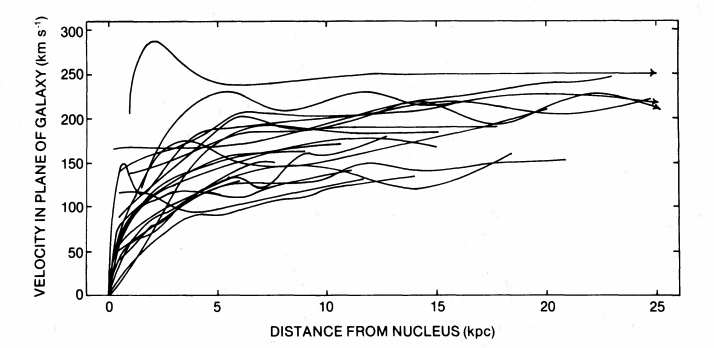
\includegraphics[width=\textwidth]{figures/theory/rot_curves.png}
\caption{Superposition of 21 rotation curves from galaxies with a large range of radii and luminosities. All galaxies have a distinctive flat rotation curve at large radii. Figure from \cite{Rubin1980}.}
\label{fig:curves}
\end{center}
\end{figure}


In order to explain the behavior of galactic rotation curves without dark matter, Milgrom proposed \ac{MOND} in a trio of 1983 papers, \cite{Milgrom1983_1}, \cite{Milgrom1983_2}, \cite{Milgrom1983_3}. Milgrom showed that if Newtonian dynamics was modified from $F = ma$ to $F= ma / a_{0}$, for a $<<$ $a_{0} \approx 1.2 \times 10^{-10} m/s^{2}$ the observed galactic rotation curves could be accounted for without requiring any hidden or dark matter. Milgrom's goal in these first papers describing \ac{MOND} was to present an approximate limit of some as-yet unknown full theory, which he and others went on to develop in the following decades \cite{Bertone2016}. However, theoretical and technological advancements in the fields of cosmology and astronomy have made \ac{MOND} an unsatisfying theory, unable to explain several observed phenomena. Of these phenomena, gravitational lensing and the \ac{CMB} are discussed further below.

Big-Bang cosmology had a large success in 1965 with Penzias and Wilsons' observation of the \ac{CMB}. It was in the 1980's however, that cosmology, particle physics, and astronomy became tied together as they are understood today, and dark matter came to refer to an as yet undiscovered particle species and not the cold gas and stars of Zwicky's day \cite{Bertone2016}. The root of this paradigm shift was in the new theory of cosmological inflation \cite{Bertone2016}. Inflation refers to a period of exponential expansion $10^{-36}$ to $10^{-33}$ seconds after Big Bang. Without an inflationary period, fluctuations would be washed out as the universe expanded, leading to a universe devoid of structure. Inflation, however, provides mechanism for quantum fluctuations to be `blown up' and seed the structure observed by the 1982 CfA redshift survey (Figure~\ref{fig:cfa}). Numerical simulations to reproduce the structure seen by the CfA redshift survey benefited from new improvements in processing speed and numerical techniques, and also from the new theory of inflation, which provided a physical reason for initial density perturbations \cite{Bertone2016}. The structure was reproduced only in the presence of gravitationally-interacting dark matter. It is interesting to note here that these cosmological simulations were largely insensitive to any additional, non-gravitational interactions the dark matter had, as long they were sufficiently weak. However, the simulations did require the dark matter to be non-relatistivc or ``cold''. Such dark matter is referred to as \ac{CDM}, and plays a prominent part in the standard cosmology to describe the structure and evolution of our universe.  

\begin{figure}[htbp]
\begin{center}
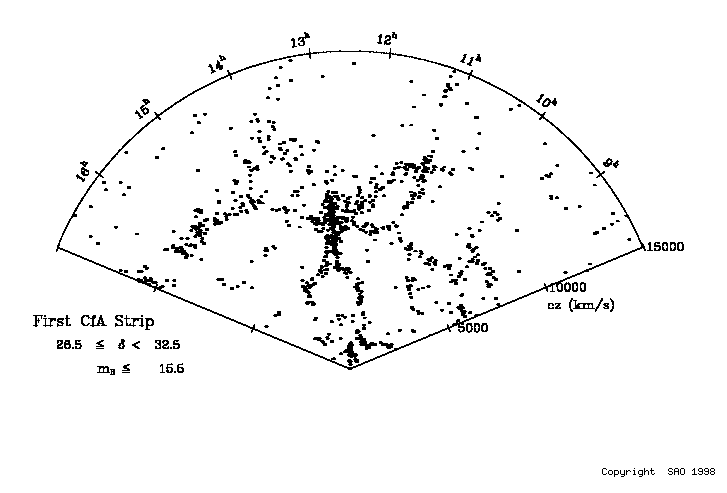
\includegraphics[width=\textwidth]{figures/theory/cfa.png}
\caption{CfA Redshift Survey result showing the distribution of galaxies in a strip on the sky about 6 degrees wide and 130 degrees long. The radial coordinate is redshift, in km/sec, calculated with a Hubble constant of 20km/sec/million ly. Figure from \cite{cfasite}. }
\label{fig:cfa}
\end{center}
\end{figure}


\section{Evidence for Dark Matter}
The previous section gave an overview of why \ac{CDM} as become, over the last century, the leading paradigm to explain the small and large-scale structure observed in our universe. The following subsections deal with particular pieces of evidence, discussed in detail.

\subsection{Galaxies and Clusters}
Galactic rotation curves were discussed above as evidence for dark matter halos. Here we further discuss the properties of dark matter halos. An example of a galactic rotation curve of a spiral galaxy showing the presence of an inferred dark matter halo is shown below in Figure~\ref{fig:rot_curve}. Each side of  Figure~\ref{fig:rot_curve} shows the same galaxy, NGC 3198, but fit with a different disk and halo model. In this particular example from 1985, the authors note their uncertainty about which halo model is the correct one: ``Should one seriously consider the case where the amount of visible matter is negligible with respect to the amount of dark matter [Figure~\ref{fig:rot_curve} (left)]? Or is the maximum disk case [Figure~\ref{fig:rot_curve} (right)] closer to the truth?" \cite{Albada1985}. A decade later, in 1996, Navarro, Frenk and White published a paper describing high-resolution simulations of \ac{CDM}, which could all be fit with a universal dark matter halo profile \cite{Navarro1996}. This formula became known as the \ac{NFW} profile; it is still widely used today, and is the basis for many direct detections experiments, including \ac{LUX}. The \ac{NFW} profile showed that Figure~\ref{fig:rot_curve} (left) is the preferred model, where the amount of dark matter far outweighs the amount of visible matter.

\begin{figure}[htbp]
\begin{center}
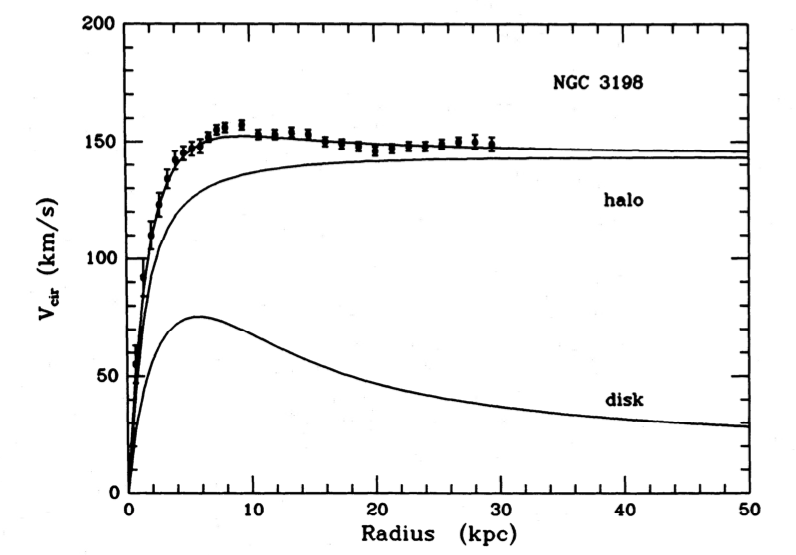
\includegraphics[width=\halffig]{figures/theory/rot_curve2.png}
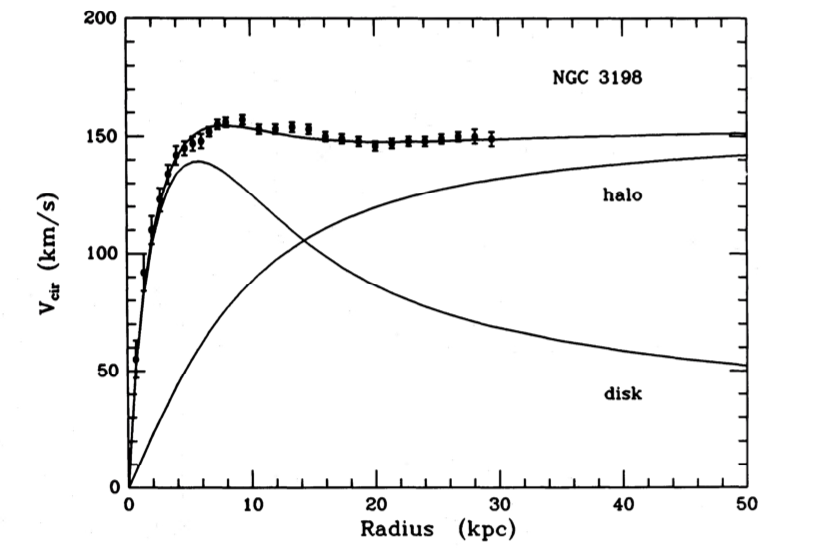
\includegraphics[width=\halffig]{figures/theory/rot_curve1.png}
\caption{Galactic rotation curve from \cite{Albada1985} fit with two different dark matter halo models. The Figure (left) is closer to the rotation curve produced by dark matter with an \acs{NFW} profile (see \cite{Navarro1996}), and our understanding of the ratio of dark matter to visible matter in most spiral galaxies. }
\label{fig:rot_curve}
\end{center}
\end{figure}

The astrophysics community is near unanimous that a galaxies have a dark matter component. Today, research continues into the particular shape of the dark matter profile. While \ac{NFW} is in common use and agrees with many observations, it is not consistent with observations of low surface brightness and dwarf galaxies \cite{DeBlok2001}, \cite{DeBlok2001a}. This known as the core-cusp problem: \ac{NFW} galaxies have an over-density of dark matter at small radius (cuspy), while dwarf galaxies favor flatter density profiles (core). Some argue that such behavior may be a consequence of the nature of dark matter, or that current simulations are not sufficient to properly understand dwarf galaxies \cite{Oman2015}. Others argue that a cusp can be changed to a core via baryonic feedback that arises in simulations of active galactic nuclei \cite{Martizzi2013}. 

Other current research into dark matter halos centers on the globular clusters and stars that orbit the Milky Way. These researchers look for evidence of halo substructure and streams of dark matter from the movements of stars orbiting the Milky Way. Data from the Gaia satellite, launched in 2013, calls into question whether dark matter halos are truly in equilibrium, which has consequences for direct detection experiments, as it would change the expected dark matter recoil spectrum \cite{Herzog-Arbeitman2018} \cite{Necib2018}. In addition to the stars and globular clusters orbiting the Milky Way, there could be clusters of dark matter more dense than the surrounding halo. Telescope data shows evidence for dark matter halo substructure in the Milky Way \cite{Erkal2017}, and simulations expect upcoming data from LSST to further contribute to the understanding of Milky Way halo substructure and rule out certain dark matter halo models \cite{Banik2018}.

Galaxy clusters make up some of the strongest direct evidence for dark matter though the method of gravitational lensing. A gravitational lens is created when a massive object is located between a light source and an observer. General relativity requires photons to propagate on the null geodesics of spacetime, meaning the path the light takes from the source will be bent by the distorted space-time of the the massive object. Thus images of background galaxies are distorted by invisible mass along the line of sight from the observer. Being dependent on general relativity, and therefore Newtonian dynamics, the numerous observations of gravitational lensing in large structures strongly disfavor \ac{MOND}. 

There are three types of gravitational lensing: strong, weak, and microlensing. Weak lensing has been used to observe dark matter in large scale structures (galaxy clusters); the other types of lensing are not treated here. In weak lensing, the light sources are far away from the foreground mass (or the mass is small). Several light sources are required, and the location of the mass is statistically reconstructed. The Bullet Cluster (1E0657-558) is one of the most dramatic weak lensing measurements to date: it is actually the collision of the galaxy cluster 1E0657-56 and smaller cluster (the ``bullet") \cite{Markevitch2001}. The x-ray image of the collision, by the Chandra x-ray observatory, shows the location of the baryonic matter. The baryonic matter suddenly slowed down upon the collision, emitting shock x-rays  \cite{Markevitch2001}. The authors of \cite{Markevitch2001} call it ``a textbook example of a bow shock", indicating the x-ray behavior is well understood. A few years later, Clowe et al. also call the Bullet Cluster ``a direct empirical proof of the existence of dark matter" \cite{Clowe2006}. Their weak lensing observations show the location of the total mass centers of the two clusters to be offset from the location of the baryonic matter at a significance of 8$\sigma$ \cite{Clowe2006}. In the collision, the dark matter halos of the two clusters pass through each other without slowing down, while the baryonic matter in the two clusters interacts, slowing down dramatically and producing x-rays. The weak lensing measurement is shown overlaid with the visible and x-ray images in Figure~\ref{fig:bullet}. Such a dramatic offset cannot be explained by modifications to gravity.

\begin{figure}[htbp]
\begin{center}
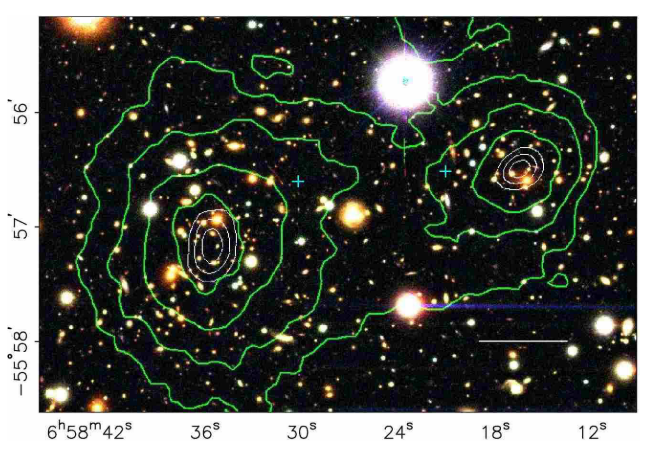
\includegraphics[width=\halffig]{figures/theory/bullet1.png}
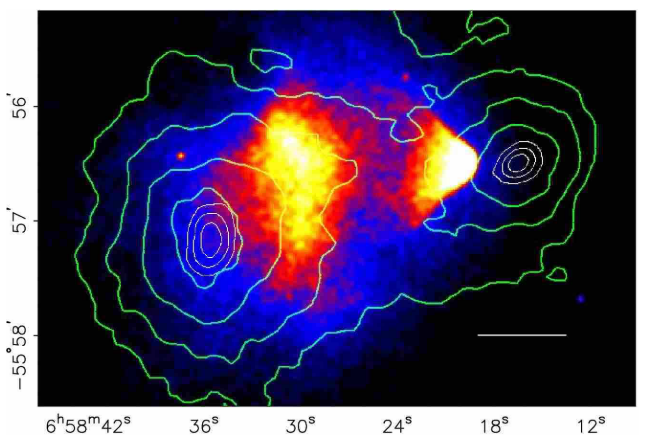
\includegraphics[width=\halffig]{figures/theory/bullet2.png}
\caption{(left) The visible light image from the Magellan telescope of the merging Bullet Cluster overlaid with the weak lensing measurement contours in green, and white 68.3\%, 95.5\%, and 99.7\% confidence levels for the weak lensing peaks. (right) The Chandra x-ray image overlaid with the same weak lensing measurement. Figure from \cite{Clowe2006}. }
\label{fig:bullet}
\end{center}
\end{figure}


\subsection{Cosmic Microwave Background}
\label{sec:cmb_dm}
In the thermal history of our universe, the term recombination refers to the epoch when temperatures had cooled enough to allow electrons and protons to combine into hydrogen, leaving photons to propagate freely through the universe. The photons should have decoupled from the matter as a black body peaked at the temperature of recombination,  $\approx$3000~K. The relic radiation from this epoch is visible today as the \ac{CMB}, where the continuing expansion of the universe has redshifted the peak of the black body spectrum to $\approx$2.7~K. The \ac{CMB} photons are also referred to as the light of last scattering, referring to the interaction the photons had with free electrons before the electrons became bound to protons in hydrogen. The temperature of the \ac{CMB} was precisely measured to be 2.7377 $\pm$ 0.0038~K  by the COBE mission, which also confirmed its perfect adherence to a black body spectrum \cite{Smoot1999} (Figure~\ref{fig:cobe}).

\begin{figure}[htbp]
\begin{center}
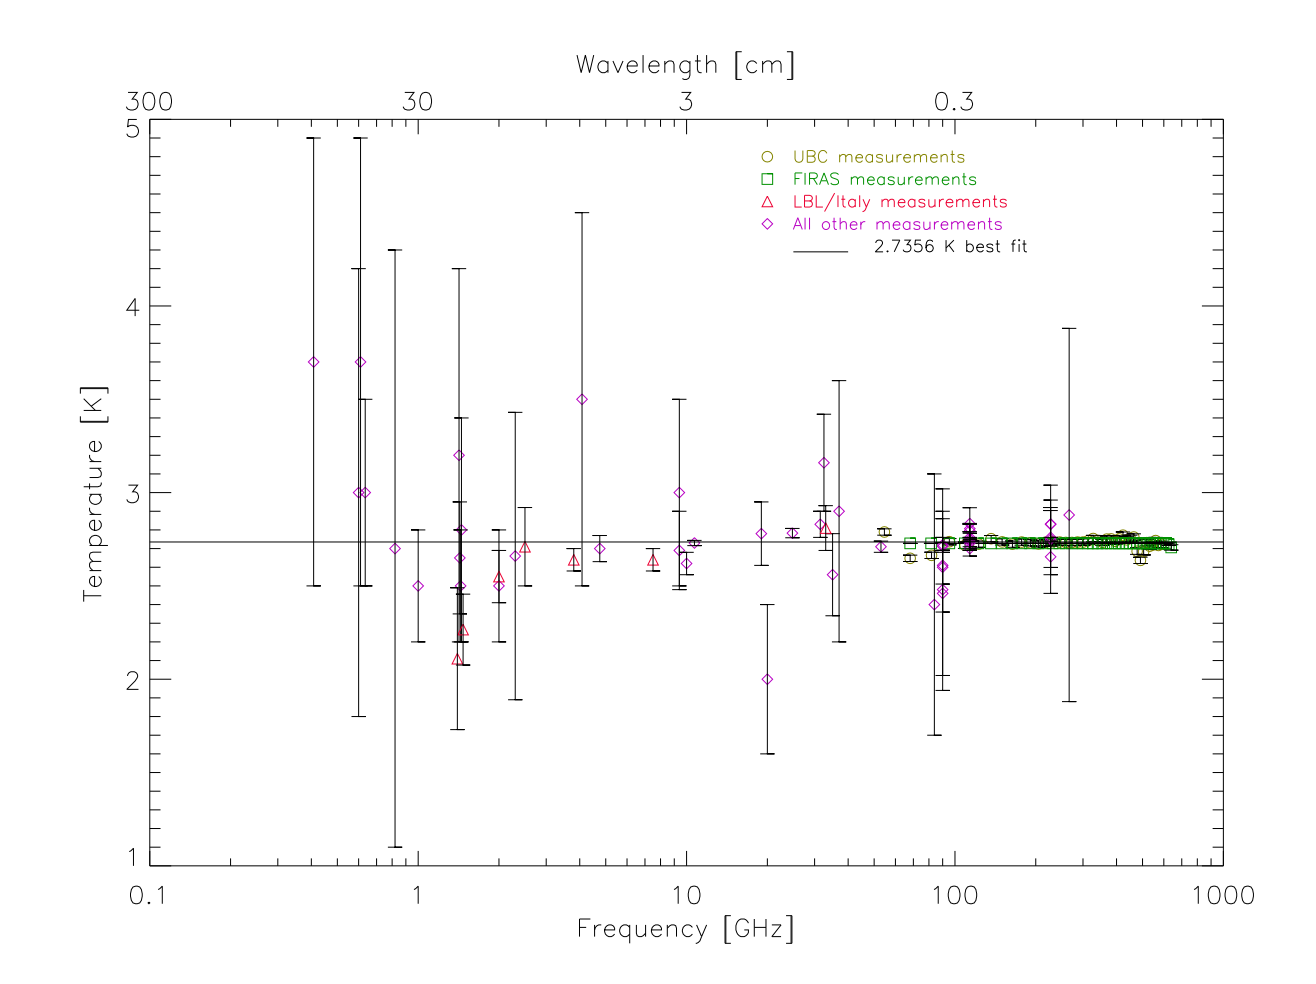
\includegraphics[width=\halffig]{figures/theory/cobe_temp.png}
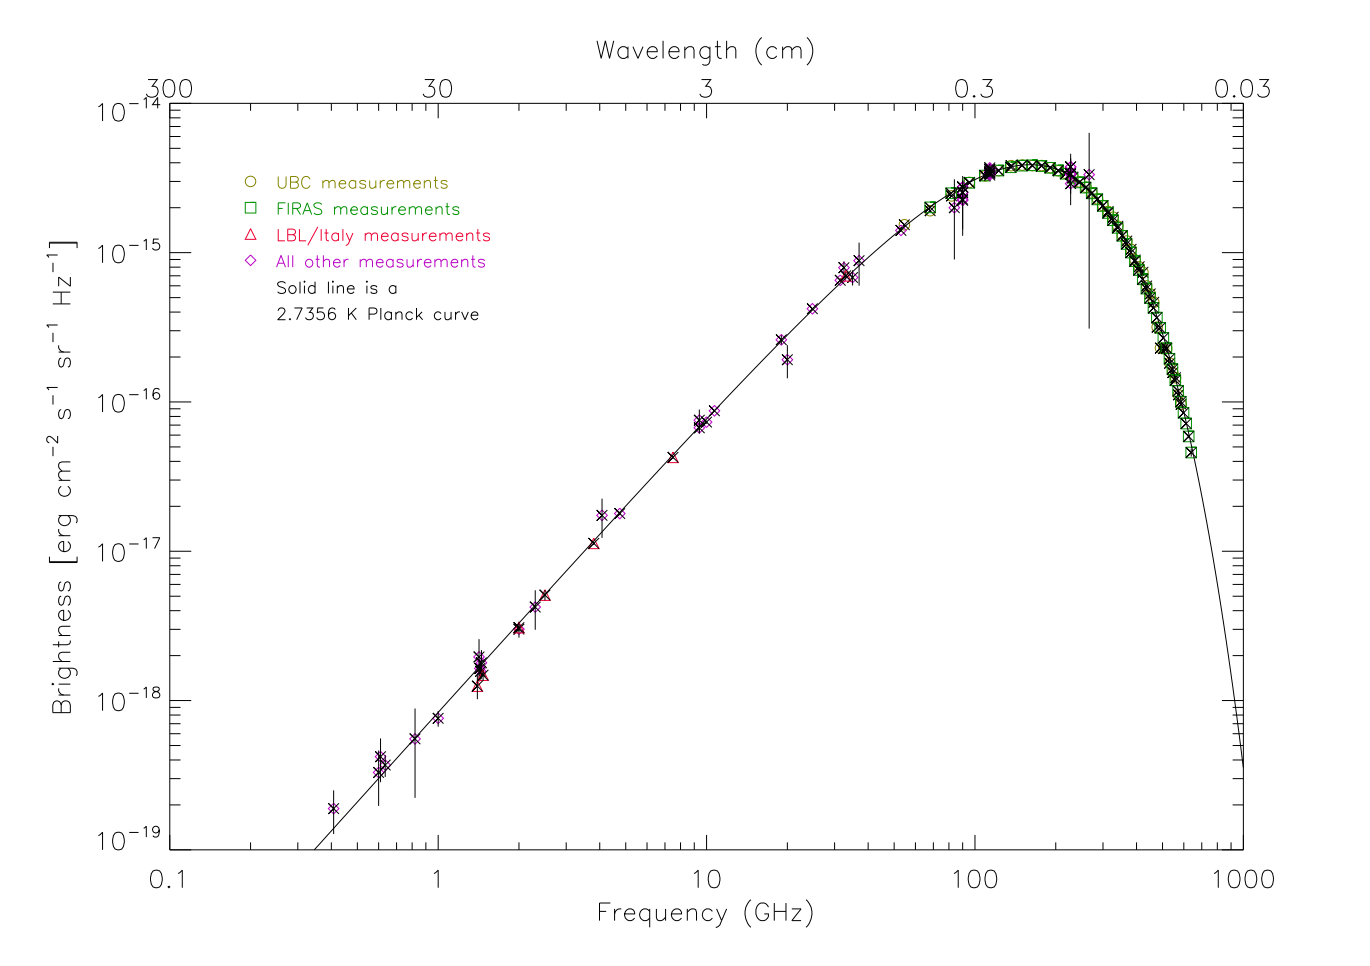
\includegraphics[width=\halffig]{figures/theory/cobe_spectrum.png}
\caption{(left) The FIRAS instrument on the COBE satellite mission measured the \acs{CMB} temperature to be 2.7377 $\pm$ 0.0038~K. (right) The FIRAS instrument also confirmed the perfect Planck black body spectral shape of the \acs{CMB} radiation. Figures from \cite{Smoot1999} }
\label{fig:cobe}
\end{center}
\end{figure}

While the COBE satellite mission's measurements of the \ac{CMB} provided strong support for the Big Bang model of cosmology, it was COBE's discovery of anisotropies in the \ac{CMB} that eventually led to powerful evidence for \ac{CDM}. Since COBE, two more \ac{CMB} satellite missions, WMAP and Planck, have launched and gathered data, each with successively higher spatial and energy resolution. The relative resolutions of COBE, WMAP, and Planck are shown in Figure~\ref{fig:cmb} along with the full Planck \ac{CMB} anisotropy map. The scale of the anisotropy fluctuations represent a scale of  $\pm$~30~$\mu$K; the \ac{CMB} power spectrum remains the most perfect black body spectrum observed in nature. 

\begin{figure}[htbp]
\begin{center}
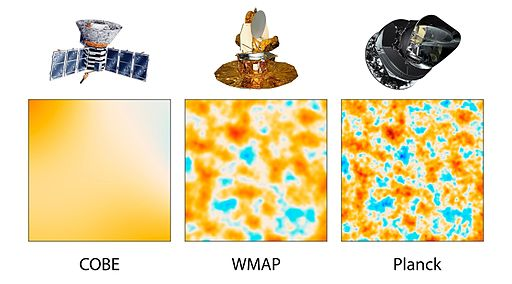
\includegraphics[width=.6\textwidth]{figures/theory/satellites.jpg}
\includegraphics[width=\textwidth]{figures/theory/planck.png}
\caption{(top) The relative spatial resolution of COBE, WMAP, and Planck. Figure courtesy of NASA. (bottom) The Mollweide projection of the Planck 2013 CMB temperature map. The color scale represents fluctuations of $\pm$~30~$\mu$K around a central value of 2.7377~K. Figure courtesy of ESA and the Planck Collaboration. }
\label{fig:cmb}
\end{center}
\end{figure}

The fluctuations $\Delta T(\theta, \phi)$ of the \ac{CMB} map shown in Figure~\ref{fig:cmb} can be decomposed into its basis components via Fourier analysis, where each expansion component is represented by the spherical harmonics, $Y_{lm}$:

\begin{equation}
\label{eq:cmb_fluct}
\Delta T(\theta, \phi) = \sum_{l=2}^{\infty} \sum_{m=-l}^{l} b_{lm} Y_{lm}(\theta, \phi)
\end{equation}

The sum leaves out the $l=0$ (mean) and $l=1$ (dipole Doppler shift caused by movement of the earth with respect to the \ac{CMB}) components, which were subtracted from the \ac{CMB} temperature map, leaving only the fluctuations as in Figure~\ref{fig:cmb}. The power spectrum of the temperature fluctuations, which is calculated by squaring Equation~\ref{eq:cmb_fluct}, averaging it over all points that have the same angular separation $\theta$, and performing an integral over all $m$ (because the temperature anisotropies have no preferred direction), encodes all the statistical variation in the \ac{CMB} sky (see, e.g. \cite{Hu2008} for a derivation). The angular correlations of the different multipole moment $l$ are typically extracted from this power spectrum and plotted as function of $l$ and the coefficients $C_{l}$ from the power spectrum. This quantity is referred to as the angular power spectrum and takes the form:

\begin{equation}
D_{l}^{TT} = \frac{ l(l + 1)}{ 2 \pi} C_{l}
\end{equation}
 
where the $TT$ superscript denotes temperature anisotropies (polarization anisotropies, not discussed here, can be parameterized similarly). The latest angular power spectrum from Planck is shown in Figure~\ref{fig:planck_multipole}.

\begin{figure}[htbp]
\begin{center}
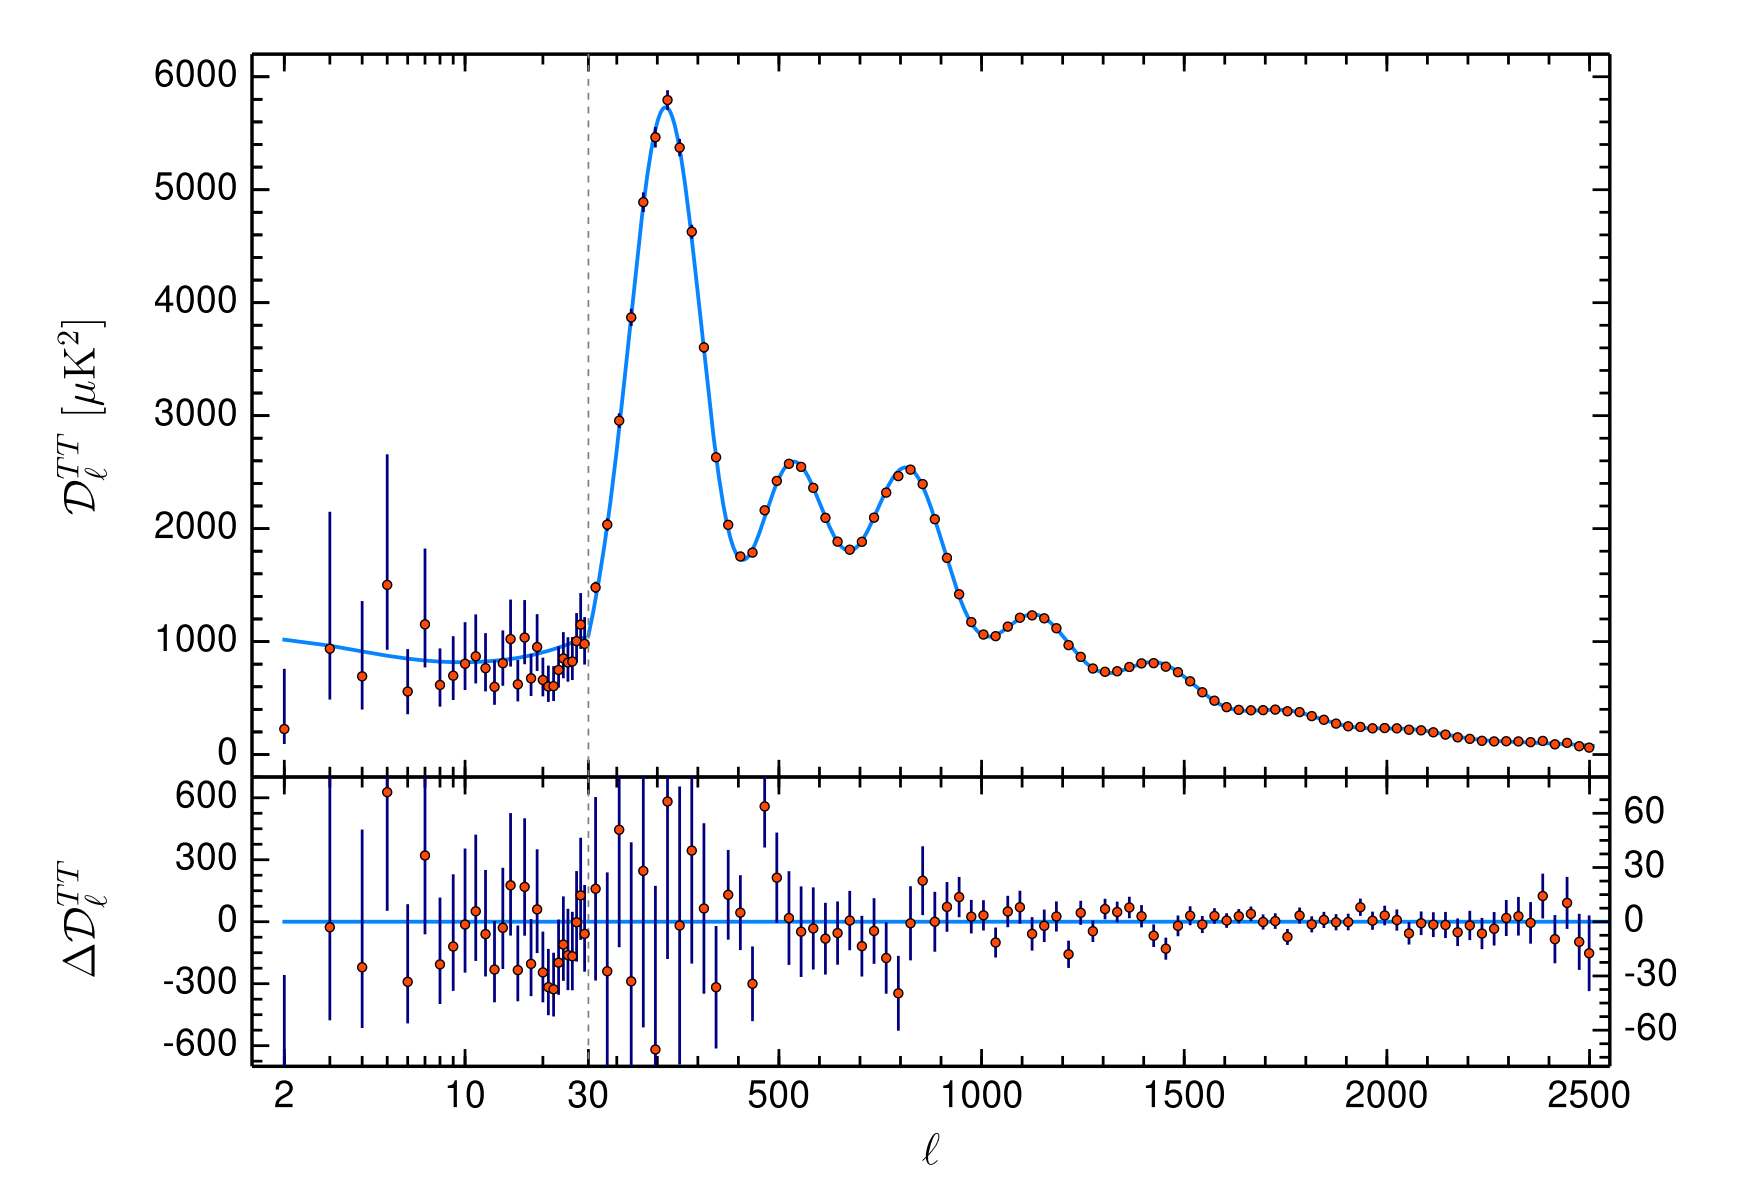
\includegraphics[width=\textwidth]{figures/theory/planck_multipole.png}
\caption{The angular power spectrum from Plank 2018 results  \cite{Planck2018}. }
\label{fig:planck_multipole}
\end{center}
\end{figure}

The location and magnitude of peaks in the angular power spectrum (Figure~\ref{fig:planck_multipole}), constrain the curvature, content, and evolution of our universe. The physical interpretation of the \ac{CMB} fluctuations is as follows: photons from the time of last scattering, newly free to propagate through the universe, carry information about the density fluctuations in the plasma from which they decoupled. The plasma, which was then composed of photons, baryons, and dark matter, behaved as an oscillator driven by gravitational attraction, with a restoring force from the fluid pressure of the plasma. The maxima of the angular power spectrum indicate extrema, overdensities or underdensities, in the plasma. The presence of baryons increases the magnitude of odd peaks relative to even peaks. The physical interpretation of this is that baryons add inertia to the oscillator system, causing an increase in compression (odd) compared to expansion (even) \cite{Hu2008}. The angular power spectrum peaks are sometimes referred to acoustic peaks, as the oscillations that produced them were longitudinal and depended on density, much like sound waves. The presence of dark matter is apparent in the relative heights of the second and third peak in the spectrum. The driving force of the oscillator is the total matter content (baryons + dark matter,) which contributes to odd peaks, while baryons contribute characteristically to the even peaks. A third peak that is similar or larger than a second peak indicates that the matter content at the time of recombination was dominated by dark matter. A useful demonstration of the effect of baryons and total matter on the angular power spectrum is shown in Figure~\ref{fig:matter_baryons}.

\begin{figure}[htbp]
\begin{center}
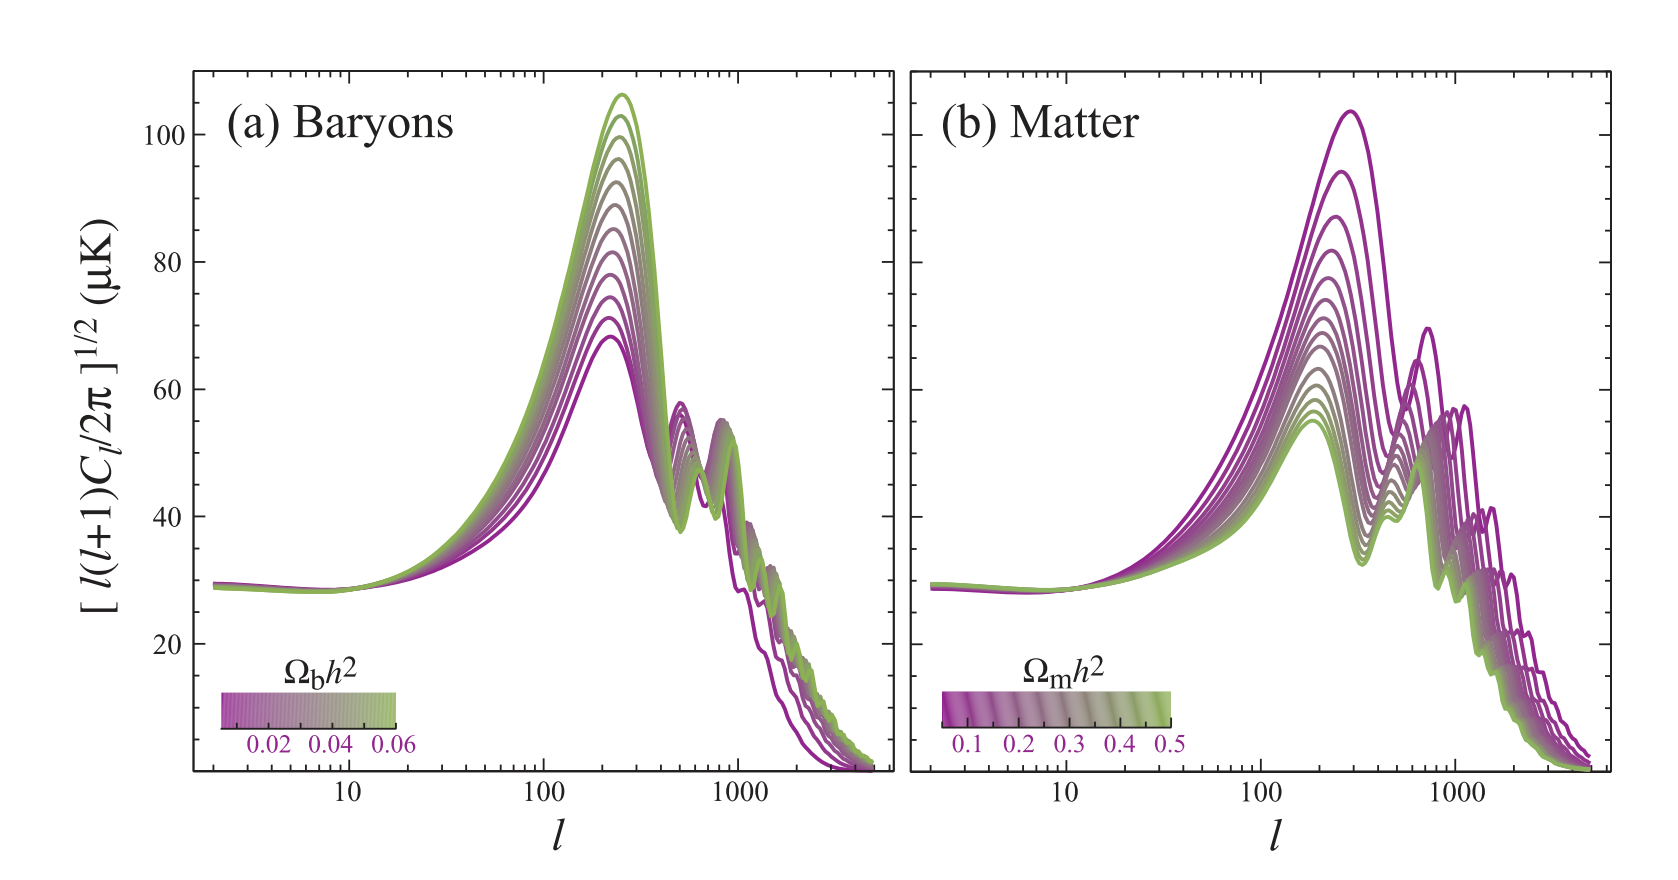
\includegraphics[width=\textwidth]{figures/theory/matter_baryons.png}
\caption{The effect of baryons (left) and total matter (right) on the magnitude and location of \acs{CMB} angular power spectrum peaks.  \cite{Hu2008} }
\label{fig:matter_baryons}
\end{center}
\end{figure}

The measure of the dark matter content and baryon content of today's universe can be extrapolated from fitting the \ac{CMB} angular power spectrum as in Figure~\ref{fig:matter_baryons}. The results from the Planck 2018 angular power spectrum (\cite{Planck2018}) are: 

\begin{equation}
\Omega_{cdm} = 0.2696 \pm 0.0047
\end{equation}

\begin{equation}
\Omega_{b}  = 0.0495 \pm 0.0005 
\end{equation}

Where the subscript $b$ refers to baryon and the subscript $cdm$ refers to cold dark matter. Each $\Omega_{x}$, defined in more detail below, represents the fraction of today's mass-energy density comprised by constituent $x$. These values do not add to one because a large fraction of the mass-energy density of the universe is comprised of dark energy, which we have left discussion of until the next section. However, note that these two values alone measure dark matter to comprise \~84\% of the matter in our universe. 


%; $h$ is the dimensionless version of the Hubble constant, $H_{0}$, which is the dominant source of error in these measurements. The Hubble constant $H_{0}$ is the ratio of the expansion of the universe to its size at $t=t_{0}$ (today). 

\section{Standard Models}
Thus far we have focused only on the astrophysical and cosmological evidence for particle \ac{CDM}. \ac{CDM} plays a central role in the standard model of cosmology, known as \ac{LCDM}. In this section, we briefly summarize the standard models of cosmology and particle physics. 


% $\Lambda$\ac{CDM} (``Lambda'' - \ac{CDM}). 
\subsection{The Standard Cosmology}
The standard \ac{LCDM} cosmology is based on the Einstein field equations:

\begin{equation}
R_{\mu \nu} - \frac{1}{2} g_{\mu \nu} R = \frac{8 \pi G}{c^{4}} T_{\mu \nu} + \Lambda g_{\mu\nu}
\end{equation}

where $R_{\mu \nu}$ is the Ricci tensor, $R$ is the Ricci scalar, and $g_{\mu\nu}$ is the metric tensor. $T_{\mu \nu}$ is the stress-energy tensor, $G$ is Newton's gravitational constant, $c$ is the speed of light in vacuum, and $\Lambda$ is the cosmological constant. The equation relates the geometry of space-time (on the left hand side) to the energy content of the universe (on the right hand side). 

Einstein originally introduced the cosmological constant $\Lambda$ to counteract gravity and produce a steady-state universe. Today, however, we know that the universe is expanding, and that the rate of expansion is accelerating. The second fact, first evidenced by supernova Type Ia measurements \cite{Riess1998} \cite{Perlmutter1998}, is what led to the modern interpretation of $\Lambda$ as dark energy. Today, we understand  $\Lambda$ to represent a ``vacuum energy'' associated with space-time itself, rather than its matter content. It is the source of the accelerating expansion of the universe, sometimes referred to as ``negative pressure'' or ``gravitational repulsion'', and it is the dominant component of mass-energy density in our universe (see Table~\ref{tb:planck}).

The Einstein field equations are solved with the Friedman-Lemaitre-Robertson-Walker metric (not shown here, see e.g. \cite{Ryden2006}, \cite{Kolb1990}), which describes the symmetries we observe in our universe and therefore require of our model: isotropy and homogeneity. The solution yields the Friedman equation (Equation~\ref{eq:friedman}), which details how the addition of different energy sources (matter, radiation, dark energy) change the expansion rate of the universe. The rate of expansion is given by the Hubble constant $H(t)$ (a slight misnomer because it can change over time scales $\sim$ history of our universe). It is defined as $H(t)^{2} \equiv \frac{\dot{a}(t)}{a(t)}$, where $a$ is the so-called scale factor, which is a dimensionless factor that parametrizes the size of the universe. The Friedman equation, given below, delineates how the Hubble constant changes with the energy content $\rho_{tot}$ and curvature $k$ of our universe.

\begin{equation}
\label{eq:friedman}
H(t)^{2} \equiv \Big( \frac{\dot{a}(t)}{a(t)} \Big) = \frac{8 \pi G}{3} \rho_{tot}(t) - \frac{k}{a(t)^{2}}
\end{equation}

The Friedman equation yields a quantity known as the critical density $\rho_{c}$, which is the density for a flat universe ($k=0$). 

\begin{equation}
\rho_{c}(t) = \frac{ 3 H(t)^{2}}{8 \pi G} 
\end{equation}

A species $x$ is defined as having a fraction of the mass-energy density $\Omega_{x}(t) = \rho_{i}(t) / \rho_{c}(t)$. The individual $\Omega_{x}$ have different time evolutions according to their equation of state (see e.g. \cite{Ryden2006}, \cite{Kolb1990}, for a complete, pedagogical treatment). After treating equations of state, the Friedman equation can be re-written in a more convenient form: 

\begin{equation}
\label{eq:Lcdm}
\frac{H^{2}}{H_{0}^{2}} = \frac{\Omega_{r, 0}}{a^{4}} + \frac{\Omega_{m, 0}}{a^{3}} + \Omega_{\Lambda, 0} + \frac{( 1 - \Omega_{tot,0})}{a^{2}} 
\end{equation}
  
where the $0$ subscript denotes today's value, $r$ denotes radtion, $m$ denotes mater, and $\Lambda$ denotes dark energy. Note that the last term disappears when $\rho_{0} = \rho_{c}$, that is, if our universe is flat. Equation~\ref{eq:Lcdm} makes a powerful statement: by measuring the energy content of the universe, we can tell the history and fate of the Universe. This is the core of\ac{LCDM} -- it is essentially a system of equations, which, when solved, can describe the history and predict the future of the universe in terms of a few measurable parameters (e.g $\Omega_{x}$). 

The Planck collaboration fits for a standard, 6 parameter \ac{LCDM}, from the \ac{CMB}. This fit includes some parameters specific to the intricacies \ac{CMB} measurements, as well as the familiar $\Omega_{x}$ density parameters from Equation~\ref{eq:Lcdm}. The 6 fit parameters\footnote{ The density parameters are often reported as $\Omega_{x}h^{2}$ since the main source of error in their measurement comes from the Hubble constant $H_{0}$. $h$ is a dimensionless parameter defined as: $h = H_{0}/( 100~km~s^{-1}~Mpc^{-1})$} are:  $\Omega_{b}h^{2}$, $\Omega_{cdm}h^{2}$, $\tau$, $ln(10^{10}A_{s})$, $n_{s}$, and $100\theta_{MC}$. Other quantities are derived from these parameters. A summary of the parameters, derived quantities, and their values is given in Table~\ref{tb:planck}. Note that the parameter $A_{s}$ is the amplitude of curvature fluctuations in the \ac{CMB} angular power spectrum (Figure~\ref{fig:planck_multipole}). The effect of baryons and dark matter on the angular power spectrum were discussed in Section~\ref{sec:cmb_dm}. Similarly, dark energy content, curvature, and equation of state of the universe also produce visible effects (see examples in Figure~\ref{fig:curve_etc}). Namely, dark energy and curvature determine the magnitude of the first peak, and curvature determines peak locations.

\begin{figure}[htb]
\begin{center}
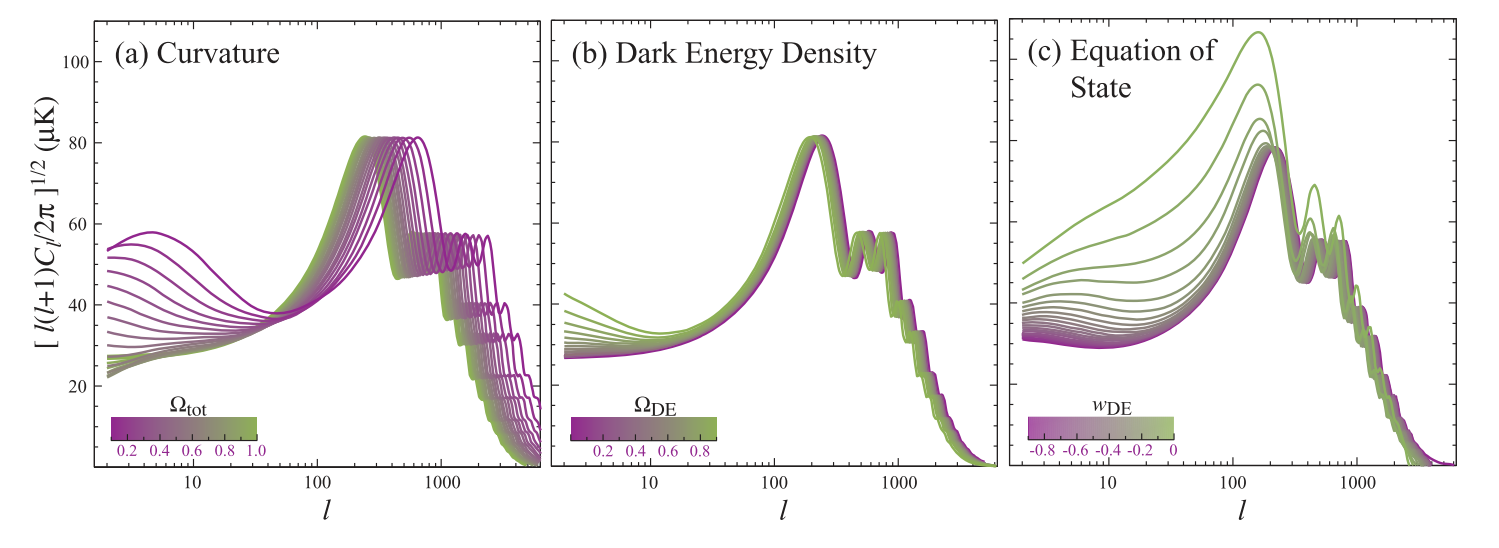
\includegraphics[width=\textwidth]{figures/theory/curve_etc.png}
\caption{The effect of curvature (left), dark energy (center), and equation of state (right) on the magnitude and location of \acs{CMB} angular power spectrum peaks.  \cite{Hu2008} }
\label{fig:curve_etc}
\end{center}
\end{figure}


\begin{table}[htbp]
\caption{A summary of the fit parameters and derived quantities from Planck's 2018 results \cite{Planck2018}.}
\begin{center}
\begin{tabular}{ r l c }
\hline
Fit Parameter & Definition &  Planck TT spectrum \\
\hline
$\Omega_{b}h^{2}$ & baryon density & 0.02212 $\pm$ 0.00022 \\
$\Omega_{cdm}h^{2}$ & CDM density & 0.1206 $\pm$ 0.0021 \\
$100\theta_{MC}$ & angular acoustic scale & 1.04077 $\pm$ 0.00047 \\
$\tau$ & optical depth & 0.0522 $\pm$ 0.0080 \\
$ln(10^{10}A_{s})$ & curvature fluctuations & 3.040 $\pm$ 0.016 \\
$n_{s}$ & spectral index & 0.9626 $\pm$ 0.0057 \\
\hline
Derived Quantity & Definition &  Planck TT spectrum \\
\hline
$\Omega_{b}$ & baryon content & 0.0495 $\pm$ 0.0005 \\
$\Omega_{cdm}$ & CDM content & 0.2696 $\pm$ 0.0047 \\
$\Omega_{m}$  & matter content & 0.321 $\pm$ 0.013 \\
$\Omega_{\Lambda}$  & dark energy content & 0.679 $\pm$ 0.013 \\
$H_{0}$ [km~s$^{-1}$~Mpc$^{-1}$] & Hubble constant & 66.88 $\pm$ 0.92 \\
Age [Gyr]  & age of the universe & 13.830 $\pm$  0.037 \\
$k$ & curvature & consistent w/ $k=0$ \\
\label{tb:planck}
\end{tabular}
\end{center}
\label{default}
\end{table}%


\FloatBarrier
\subsection{The Standard Model of Particle Physics}
The \ac{SM} of particle physics describes all the currently known matter particles and force carrier particles, which can also have mass, and which dictate interactions between the matter particles. As of 2012, it also includes a mass generation mechanism from the Higgs boson. The \ac{SM} is formulated using the principles of Quantum Field Theory, where symmetries in the Lagrangian give rise to conserved physical quantities and thereby determine the rules for interactions.

\begin{figure}[htbp]
\begin{center}
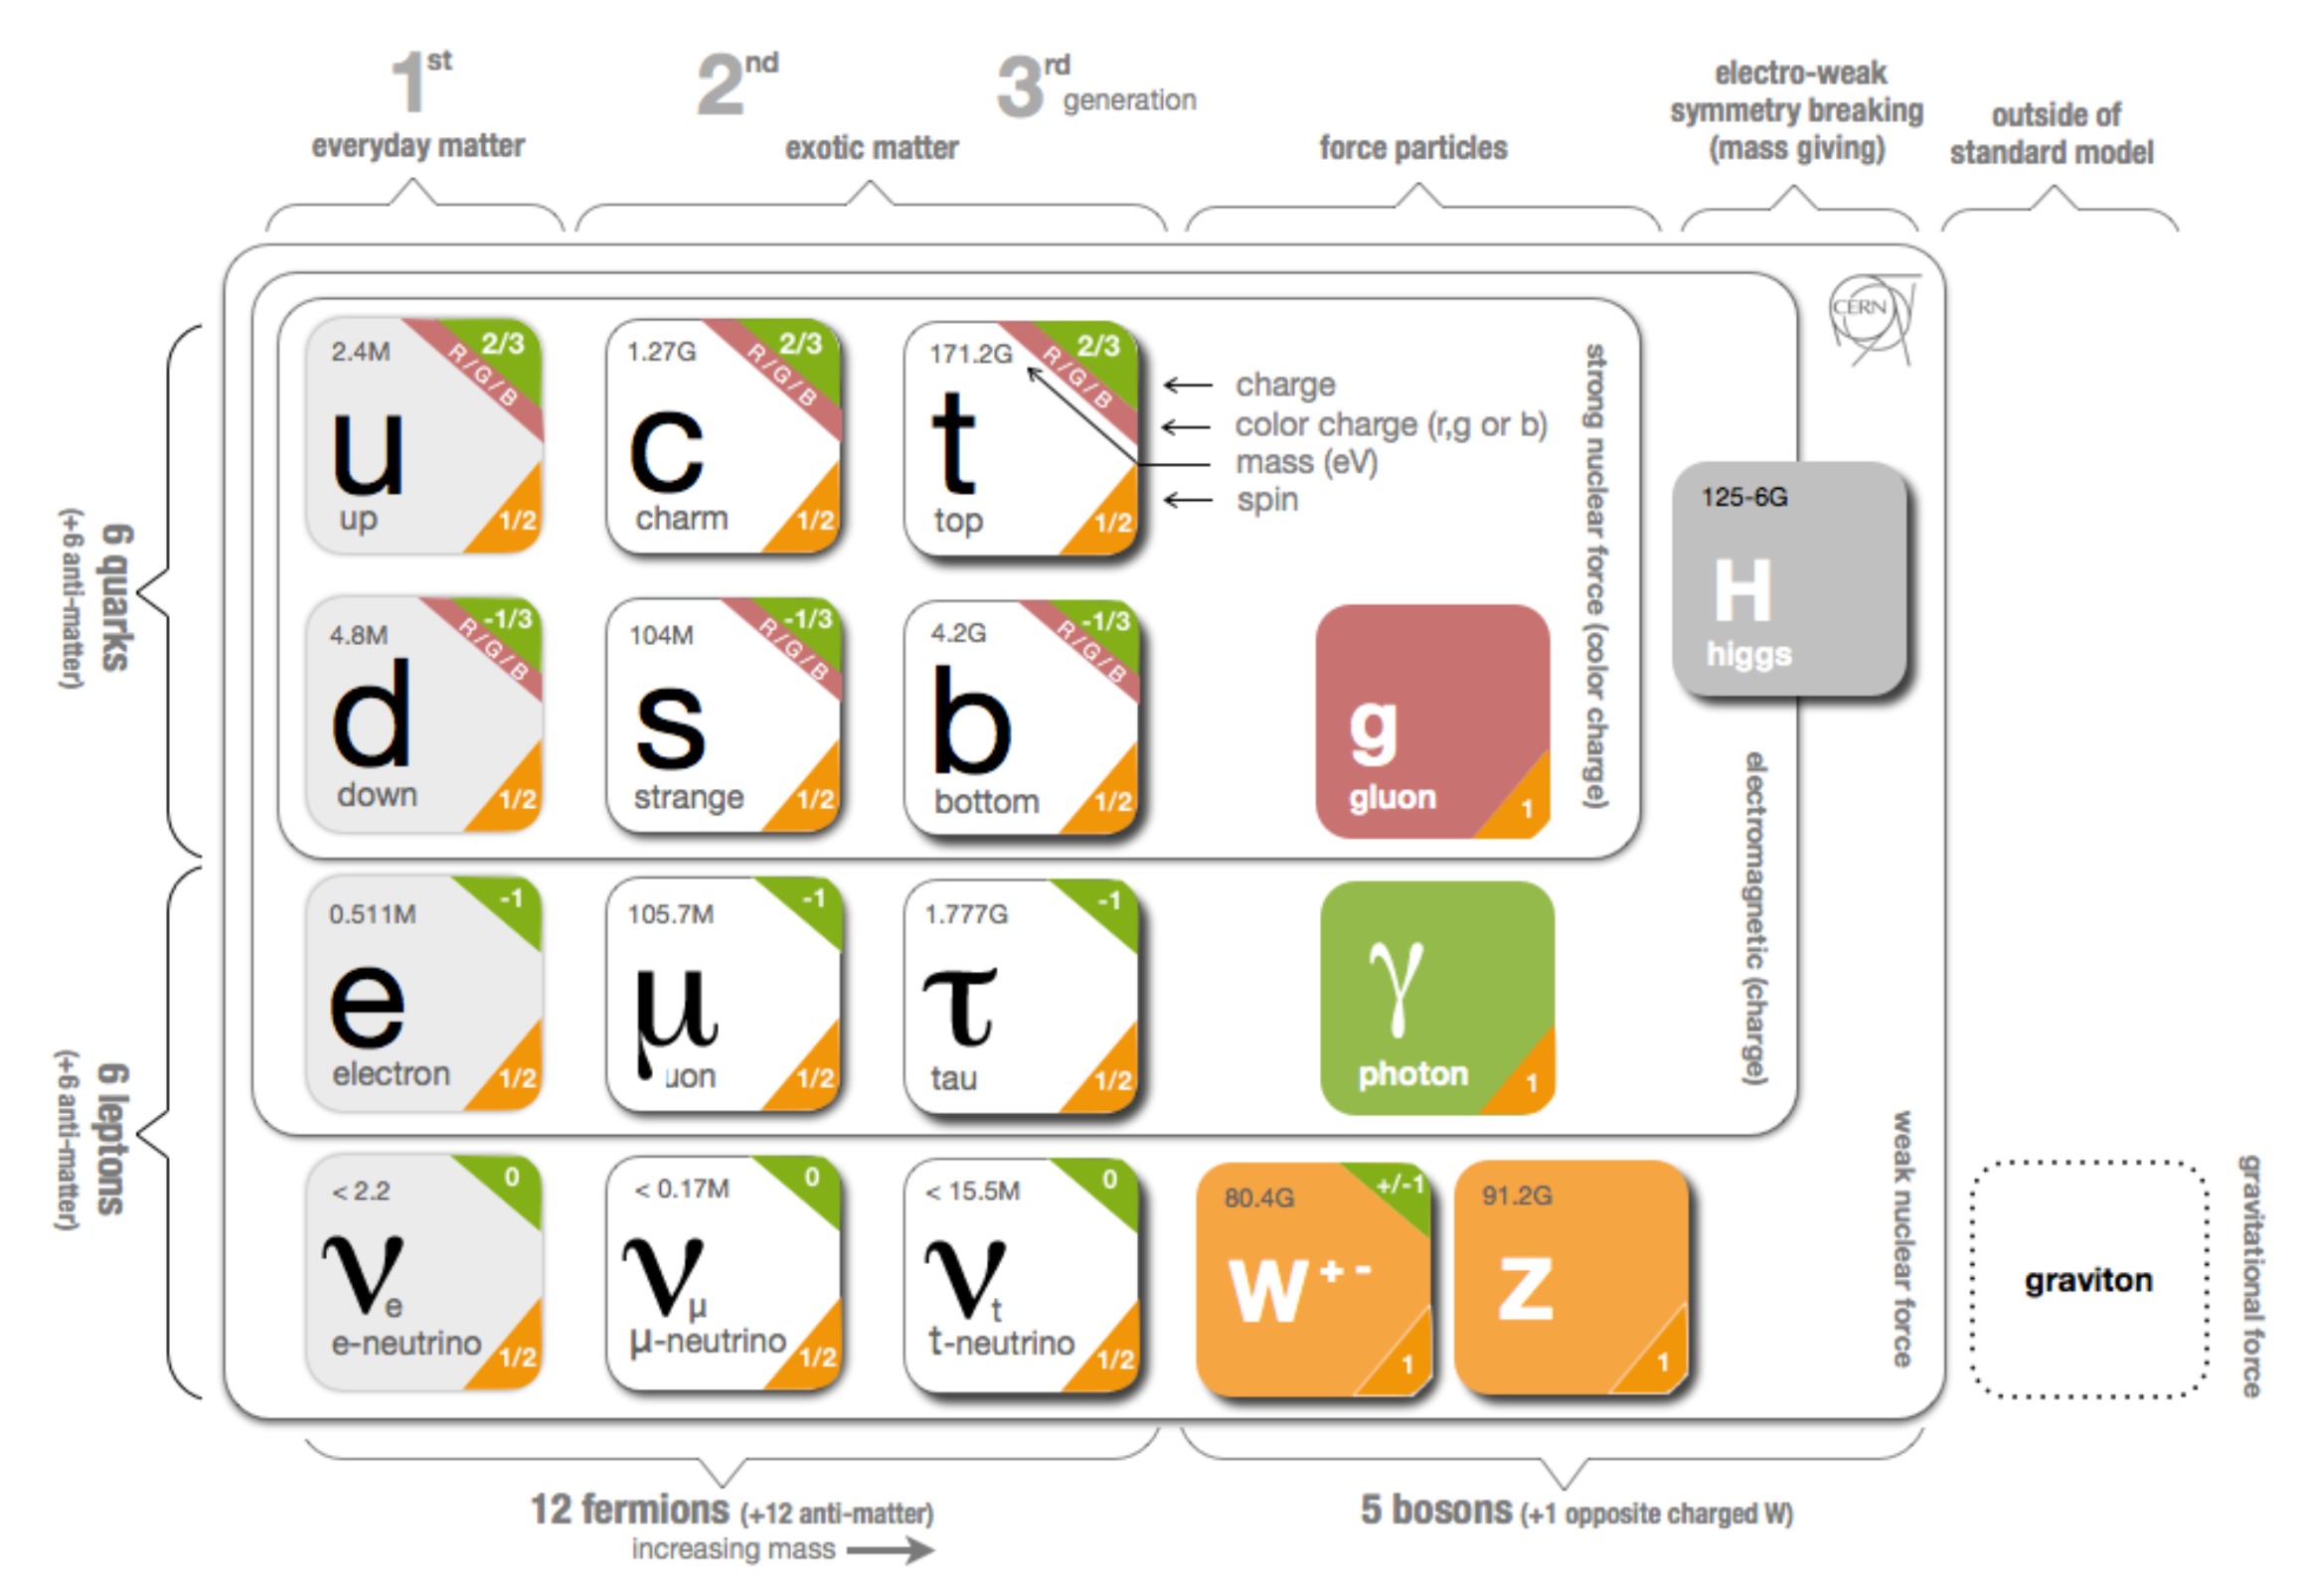
\includegraphics[width=\textwidth]{figures/theory/sm.png}
\caption{The particles that comprise the standard model of particle physics, including names, spins, masses, and charges. It is also indicated which fermions interact with which bosons, e.g. gluons interact with the quarks but not with the leptons. }
\label{fig:sm}
\end{center}
\end{figure}


The known particles of the \ac{SM} are shown in Figure~\ref{fig:sm}, along with a theoretical force carrier for gravity, the graviton. These particles are typically grouped into categories: fermions and bosons. Fermions comprise all the known matter particles and are spin-$\frac{1}{2}$ particles. Each of the fermions in Figure~\ref{fig:sm} has an anti-particle, although it is an open question whether the neutrino is its own anti-particle. The integer-spin bosons, excepting the Higgs boson, which provides a mechanism for giving mass to all the other particles, are the force carriers of the standard model. The spin-1 bosons: the gluon, photon, and $W$ and $Z$ boson, describe three of the four forces known to physics. The gluon mediates the strong force, which governs interactions between quarks, binding them in hadrons (three quark states which make up e.g. protons and neutrons) and mesons (two-quark states such as pions). The photon mediates electromagnetism, governing interactions between particles with electric charge. The $W^{+}$, $W^{-}$, and $Z$ bosons mediate the weak force, which includes phenomena such as beta-decay and neutrino-electron scattering.

It was once proposed that the $Z$ boson could mediate the interaction between \ac{DM} and \ac{SM}, because a \ac{DM} particle that interacts via the weak force fits the \ac{WIMP} paradigm discussed below. However, direct detection experiments have long excluded such scattering cross sections, of $\~10^{-39}$~cm$^{2}$. Naively, it is possible for neutrinos, which interact weakly and have mass, to be \ac{CDM}. However, neutrinos were relativistic during structure formation so could not perform the role of necessary of \ac{CDM}. Estimates of the density of today's relic neutrinos show that $\Omega_{v} \approx (1.2 - 2.2) \times 10^{-3} << \Omega_{cdm}$ \cite{Quigg2008}, \cite{Hannestad2004}. The standard model, as it is known today, contains no particles that could be \ac{CDM}. 

\section{Dark Matter Candidates Motivated by Particle Physics}
Cosmology, while providing very precise measurements of the dark matter content of the universe, essentially requires only three things of dark matter candidates: (1) the candidate must account for the observed $\Omega_{cdm}$, (2) at least 95\% of it is non-relativistic or ``cold'' \cite{Viel2005}, (3) it is not strongly self-interacting (``collisionless'') or strongly interacting with baryons. Requirement (1) is fairly loose, as it is possible for multiple different dark matter particles to comprise together $\Omega_{cdm}$, but note that it implies the dark matter candidate(s) must be stable on the timescale of the universe, or there must be a production mechanism to create the necessary abundance seen today. This section briefly summarizes two very different dark matter candidates, which have additional motivation due to open questions from the standard model. 

\subsection{WIMPs and the Hierarchy Problem}
\label{sec:wimp_miracle}
Any system that describes particle interactions today at ``low energy'', should also scale to describe particle interactions at different times (and therefore energies) in the history of our universe, namely in the first 10$^{-43}$ seconds after the Big Bang in a time known as the Planck epoch. During the Planck epoch, energies were at the Planck scale of $10^{19}$~GeV, and gravitational interactions become as large as the other forces. Any sound quantum theory should be able to account for gravitational interactions at this energy scale. However, the highest energies described by the \ac{SM} is the known as the electroweak scale, when electromagnetism and the weak force unify. The breaking of the electroweak symmetry is done by the Higgs mechanism, which provides mass. There is a compelling argument that the strong and electroweak forces unify at energies referred to as the \ac{GUT} scale, and that this theory then unifies with gravity at the Planck scale (sometimes called ``Theory of Everything'') \cite{Dimopoulos1991}. The 16 orders of magnitude between the Planck scale and the electroweak scale is known as the Hierarchy Problem; there must be new physics between the electroweak scale and the Planck scale, i.e new particles with $m > m_{Higgs}$ and new symmetries, to properly describe particle interactions during the history of our universe.

In order to solve the Hierarchy Problem, a framework known as \ac{SUSY} was developed. In \ac{SUSY} each \ac{SM} particle has a ``superpartner.'' In general, the superpartners have a spectrum of masses higher than \ac{SM} particles and a symmetry called $R$-parity partitions and limits interactions between \ac{SM} and \ac{SUSY}. The lightest of the \ac{SUSY} particles, called the \ac{LSP}, can be stable. If the \ac{LSP} is neutrally charged, then it is a \ac{WIMP} dark matter candidate.

The \ac{WIMP} paradigm has its roots in the mathematical coincidence called the ``\ac{WIMP} Miracle''. If one assumes a weak-scale coupling and mass for dark matter, it naturally produces the entire $\Omega_{cdm}$ observed today via thermal freezeout. When the universe was small and dense with particles, a \ac{WIMP}, $\chi$, would meet its antiparticle $\bar{\chi}$ and annihilate into lighter particles: $\chi \bar{\chi} \rightarrow l \bar{l}$. The reverse reaction to produce the heavier \ac{WIMP} ($ l \bar{l} \rightarrow \chi \bar{\chi} $) proceeds as long as the energies of the particle is sufficiently high, i.e. $T > m_{\chi}$. When this condition is met, the number density $n$ of \ac{WIMP}s is at its thermal equilibrium value $n_{eq}$. As the universe expands, the reaction falls out of thermal equilibrium. Both directions of the reaction ($\chi \bar{\chi} \rightleftharpoons l \bar{l}$) are affected: the reverse reaction cannot produce more $\chi$ due to cooling, and the forward reaction stalls because annihilation rate $\Gamma_{A}$ relies on a sufficiently high number density $n$, such that the probability of $\chi$ to meet $\bar{\chi}$ is large. The number density of \ac{WIMP}s become frozen into a relic density that we can observe today when the Hubble expansion rate overcame the annihilation rate:

\begin{equation}
\begin{split}
H(t) &> \Gamma_{A} \\
 &> n_{\chi} \langle \sigma_{A} v \rangle
\end{split}
\end{equation}

where $\langle \sigma_{A} v \rangle$ is the thermally averaged annihilation cross section. The time when $H(t) = \Gamma_{A}$ is referred to as freezeout. Following \cite{Feng2010}, the time evolution of the number density is described by the Boltzmann equation (see Figure~\ref{fig:wimp_miracle} (left) for number density evolution before and after freezeout):

\begin{equation}
\frac{dn}{dt} = -3 H n - \langle \sigma_{A}v \rangle (n^{2} - n_{eq}^{2} )
\end{equation}

This equation must be solved numerically (a more complete analysis can be found in e.g. \cite{Lisanti2016}), but making a few assumptions, \cite{Feng2010} finds:

\begin{equation}
\begin{split}
\Omega_{\chi} &\sim \frac{m_{\chi} T_{0}^{3}}{ \rho_{c}} \frac{n_{f}}{T_{f}} \\ %\approx  \frac{20 T_{0}^{3}}{ \rho_{c} M_{Pl} } \langle \sigma_{A}v \rangle^{-1}  \end{equation}
&\propto [\mathrm{constants}] \langle \sigma_{A}v \rangle^{-1} 
\end{split}
\end{equation}

Where $\rho_{c}$ is the critical density, $f$ subscripts refer to freezeout and $0$ subscripts refer to today's values. $\Omega_{\chi}$ then depends only on the particular annihilation cross section, which is set by the mass scale $m_{\chi}$:

\begin{equation}
\label{eq:sigmav}
\sigma_{A}v = k \frac{g_{weak}^{4}}{16 \pi^{2}m_{\chi}^{2}} ( \mathrm{1~or}~v^{2} ) 
\end{equation}

Where $v^{2}$ is present or absent for S- or P-wave annihilation and $k \sim \frac{1}{2} - 2$ parameterizes the deviation of $g$ from $g_{weak} \approx 0.065$. If the mass of the dark matter particle is in the range $m_{\chi} \sim$ 100~GeV-1~TeV, then $\Omega_{\chi}$ accounts for 100\% of today's observed $\Omega_{cdm}$. This is the \ac{WIMP} miracle: weak-scale particles can account for \textit{all} the dark matter content. Even if the \ac{WIMP} mass $m_{\chi}$ deviates from this perfect situation, the particle can still make up a substantial percentage of dark matter (see Figure~\ref{fig:wimp_miracle} (right)),

\begin{figure}[htbp]
\begin{center}
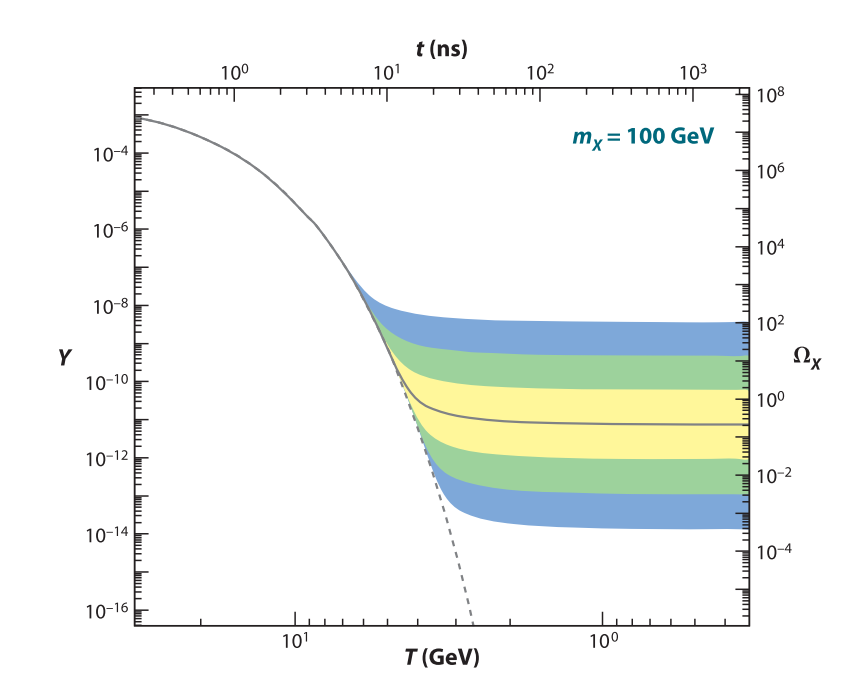
\includegraphics[width=\halffig]{figures/theory/freezeout.png}
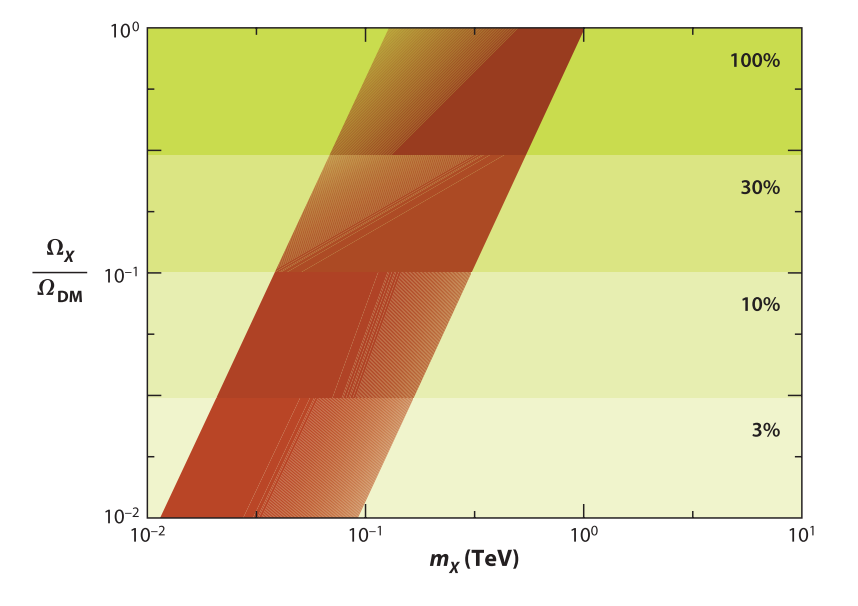
\includegraphics[width=\halffig]{figures/theory/wimp_miracle.png}
\caption{(left) The co-moving number density $Y$ (left y-axis) resulting in the thermal relic density $\Omega_{\chi}$ (right y-axis) for a dark matter particle of mass $m_{\chi}$=100~GeV. The solid black line is the annihilation cross section which yields the correct relic density and bands indicate cross sections that differ by successive factors of 10 from the ``correct'' annihilation cross section. (right) A band of natural values for a thermal relic $\chi$ that composes different percentages of the observed dark matter content. The width of the band is set by the deviation of $g$ from $g_{weak}$ in Equation~\ref{eq:sigmav}. Figures from \cite{Feng2010}}
\label{fig:wimp_miracle}
\end{center}
\end{figure}

A particle with the exact mass and weak-scale coupling, i.e scattering mediation via the Z-boson, has been ruled out by direct detection experiments, but various \ac{SUSY} parameter regions remain. The \ac{LSP} can be a \ac{WIMP}, and thereby it could solve two mysteries of physics: the hierarchy problem, and dark matter. 

\subsection{Axions and the Strong CP Problem}
\label{sec:axion}
The \ac{SM} includes a term in the quark sector that should contribute to CP-violating, flavor-conserving observables that scale with a mixing angle $\theta_{3}$:

\begin{equation}
\mathcal{L} = \theta_{3} \frac{g_{3}^{2}}{32 \pi^{2}} G^{\mu \nu}_{a} \tilde{G}_{a \mu \nu}
\end{equation}

where $g_{3}$ is the gluon coupling constant, $G^{\mu \nu}_{a}$ is the gluon field strength, and $\theta_{3}$ is a dimensionless constant.

This term should produce, for example, an electric dipole moment of the neutron, $d_{e}$. For natural values of $\theta_{3} \sim 1$,  one would expect $d_{e} \sim10^{-16}$~e~cm. However, such a dipole moment has never been observed and current experimental limits constrain $d_{e} < 2.9 \times 10^{-26}$~e~cm \cite{Feng2010}. To account for this, $\theta_{3}$ must be `fine tuned' to $\theta_{3} \longrightarrow \theta_{3}10^{-10}$. This is known as the Strong-CP Problem: we expect CP-violating observables from the \ac{SM}, but instead we find that CP is strongly conserved.

In 1977 Peccei and Quinn proposed a mechanism that solves the strong CP problem: a new hidden and spontaneously broken global symmetry allows $\theta_{3}$ to be a dynamical value which goes to zero when the symmetry is broken. A spontaneously broken global symmetry generates a Goldstone boson, so there is a new particle with non-zero mass called the axion (or QCD axion). Although they are predicted to be light ($\sim \mu$eV to meV), axion production is possible in the early Universe in such a way that they can be \ac{CDM}. Depending on whether the Peccei-Quinn symmetry is broken before or after cosmological inflation, different constrains apply. In either case it is possible for an axion with the appropriate mass to make up all of the $\Omega_{cdm}$ observed today \cite{PDGAxions2017}.


\section{The Dark Sector and Lightly Ionizing Particles}
\label{sec:dark_sector}
Chapter~\ref{ch:lips} of this thesis details a search for \ac{LIP}s, in this section the theoretical underpinning of such a particle is discussed. 

\subsection{Dark Sector}
Our universe is dominated by non-baryonic dark matter. A simple way of explaining dark matter without modifying the existing \ac{SM} is to require the existence of a dark sector (also called hidden sector), which interacts with the visible sector primarily through gravity \cite{Foot2014}. In general, there may me multiple dark sectors, each with structure rich enough to rival that of the \ac{SM}. The dark sector and and visible sector may have different thermal histories, but the size of the dark sector (counted in degrees of freedom) is still constrained by the cosmological history we observe in the visible sector. If the hidden sector and visible sector have equal temperatures at the time of \ac{BBN}\footnote{\ac{BBN} is the time when the the universe has cooled enough to allow the nuclei of the light elements to form ($t_{BBN}\sim$1-1000~s). For more in-depth and pedagogical discussion of \ac{BBN} and what constrains it places see e.g. \cite{Ryden2006}, \cite{Kolb1990}.}, an exact copy of the \ac{SM} is excluded. If the hidden sector and visible sector do not have the same temperature at \ac{BBN}, either because they are not in thermal contact or they cool independently after inflation, hundreds of degrees of freedom, equivalent to several copies of the \ac{SM} are allowed \cite{Feng2010}.

Dark sectors arise in many extensions to the \ac{SM} to provide viable dark matter candidates, such as (pseudo-)scalars that appear naturally when symmetries are broken at high energy scales. If that sounds familiar, it is because an example of such a dark matter candidate, the QCD axion, was discussed above. Aside from gravity, symmetry requirements restrict the interactions the dark sector particles may have with the \ac{SM} to a few interactions. These interactions provide what is known as a ``portal'' to the \ac{SM}. In general, a dark sector may be completely hidden with no interactions other than gravity with the \ac{SM}, but some portals are well-motivated by theoretical concerns \cite{Essig2013} \cite{Feng2010}. In some cases a portal is even required in order to explain galactic structure formation \cite{Foot2014}. Four portals that are discussed often with in respect to dark sectors are shown in Table~\ref{tb:portals} \cite{Essig2013}.

\begin{table}[htp]
\caption{Possible dark sector portals, related dark matter candidates, and operators that connect the dark sector to the \acs{SM}. Table from \cite{Essig2013}. }
\begin{center}
\begin{tabular}{ c c c }
Portal Name & Dark Matter Candidates &  Operator(s) \\
\hline
Vector & Dark Photons or LIPs & $\frac{\theta}{2} F^{\mu \nu} F^{\prime \mu\nu}$ \\
\multirow{3}{*}{Axion} & \multirow{3}{*}{Pseudoscalars} & $\frac{a}{f_{a}} F_{\mu \nu} \tilde{F}^{\mu \nu}$, \\
& & $\frac{a}{f_{a}} G_{i\mu \nu} \tilde{G}_{i}^{\mu \nu}$,  \\
& & $\frac{\partial_{\mu}a}{f_{a}} \bar{\psi}\gamma^{\mu}\gamma^{5} \psi $ \\
Higgs & Dark Scalars & $(\mu S +\lambda S^{2})H^{\dagger}H $ \\
Neutrino & Sterile Neutrinos & $y_{N}LHN$ \\
\label{tb:portals}
\end{tabular}
\end{center}
\label{default}
\end{table}%

Higgs portal and neutrino portal searches are best suited to high-energy collider searches and neutrino facilities, respectively. Axion and vector portal searches can also be accomplished with these technologies, but direct detection offers low cost alternatives that are also model-independent. Such detection schemes are discussed more below, in Section~\ref{sec:dm_detection_schemes}. The axion described in Section~\ref{sec:axion} is referred to as the QCD axion, it has a specific combination of axion mass and axion-\ac{SM} coupling. More general axion models, called \ac{ALP}s, are less constrained and can make up some percentage of \ac{DM} \cite{Essig2013}. The vector portal is characterized by a dark photon (``paraphoton'' in older texts), $A^{\prime}$, that kinetically mixes with the \ac{SM} photon, $A$. The mixing strength is parametrized by a factor $\theta$. Dark photon dark sectors are broken up into two cases: $m_{A^{\prime}} = 0$, and $m_{A^{\prime}} > 0$. For the massive dark photon case ($m_{A^{\prime}} > 0$), the dark photon itself can be dark matter. In the simplest case for the vector portal, the dark sector only consists of a massive dark photon and no other particles. Models exist for $m_{A^{\prime}} \sim$~MeV-GeV range as well as the sub-eV range \cite{Essig2013}.

In case where the dark photon is massless ($m_{A^{\prime}} = 0$), other hidden sector particles $h$ can be stable and massive. This case is yields \ac{LIP}s, discussed in the next section.

\subsection{Lightly Ionizing Particles}
Lightly ionizing particles, also known as milli- or fractionally-charged particles, stem from massless dark photon models. The kinetic Lagrangian includes the terms \cite{Holdom1986} \cite{Abel2008}:

\begin{equation}
\label{eq:Ldark}
\mathcal{L} \supset -\frac{1}{4g^{2}}F_{\mu\nu}F^{\mu\nu} - \frac{1}{4g^{\prime2}}F^{\prime}_{\mu\nu}F^{\prime \mu\nu} + \frac{\theta}{2gg^{\prime}} F_{\mu\nu}F^{\prime \mu\nu}
\end{equation}

Where $F_{\mu\nu} = \partial_{\mu}A_{\nu} - \partial_{\nu}A_{\mu}$ is the usual electromagnetic field tensor, and $F^{\prime}_{\mu\nu}$ is similarly the field tensor for the dark photon. The last term is called the kinetic mixing term, as it mixes the gauge kinetic terms for each sector. 

Let $h$ be a hidden sector fermion field that has a bare coupling to the hidden photon $A^{\prime}$, such that

\begin{equation}
\mathcal{L} \supset \bar{h}\slashed{A}^{\prime} h 
\end{equation}

where we use the Feynman slash notation ($\slashed{X} \equiv \gamma^{\mu}X_{\mu}$). The kinetic mixing term in Equation~\ref{eq:Ldark} can be diagonalized by the shift:

\begin{equation}
A^{\prime}_{mu} \longrightarrow \tilde{A^{\prime}}_{mu} + \theta A_{\mu}
\end{equation}

With the shift, the hidden sector fermion $h$ now couples to the photon:

\begin{equation}
\mathcal{L} \supset \bar{h}\slashed{A}^{\prime} h \longrightarrow  \bar{h}\tilde{\slashed{A}}^{\prime} + \theta \bar{h} \slashed{A} h
\end{equation}

The last term in the equation above corresponds to an effective coupling $q$ of the hidden sector particle $h$ with the visible photon $A$: 

\begin{equation}
q = \theta g^{\prime} \equiv \epsilon
\end{equation}

In general, $g^{\prime}$ can be large, but $\theta$ is constrained to be small (otherwise the sector would not be hidden). An example diagram of $h$ interacting with electrons is shown in Figure~\ref{fig:diagram}. The electrons only ``see'' $h$ through the $A^{\prime}$ coupling with $A$, and thus $h$ appears with a small, non-integer charge with respect to the visible sector. The magnitude of the diagram goes as the three couplings:

\begin{equation}
|M| \sim  \theta g^{\prime} g = \theta g^{\prime} e \equiv \epsilon e
\end{equation}

where we substituted the known low-energy \ac{QED} gauge coupling $e$ for $g$. The particle $h$ is known as a \ac{LIP}, and can treated as having $\epsilon e$ charge in encounters with \ac{SM} electrons.
There are many constraints on \ac{LIP}s from various sources summarized in Figure~\ref{fig:lip_constraints}, taken from a 2009 review article on fractionally charged particles \cite{Perl2009}.

\begin{figure}[htbp]
\begin{center}
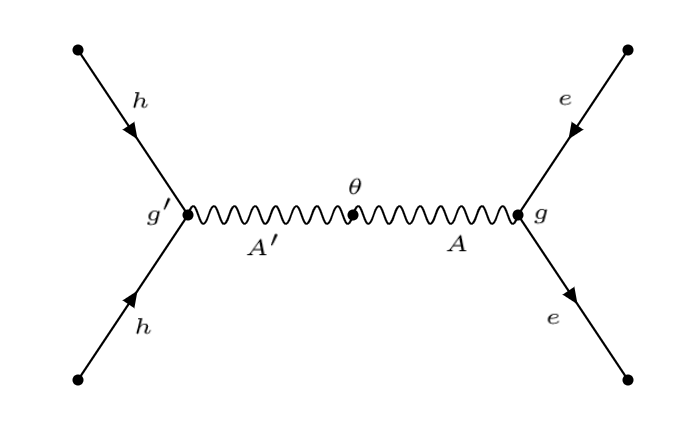
\includegraphics[width=0.8\textwidth]{figures/theory/diagram.png}
\caption{ A Feynman diagram of a dark sector particle $h$ interacting with atomic electrons. $g^{\prime}$ is the gauge coupling to $A^{\prime}$ in the dark sector, $\theta$ the kinetic mixing angle between $A^{\prime}$ and $A$, and $g$ is the usual electromagnetic gauge coupling, $g=e$.  }
\label{fig:diagram}
\end{center}
\end{figure}


\begin{figure}[htbp]
\begin{center}
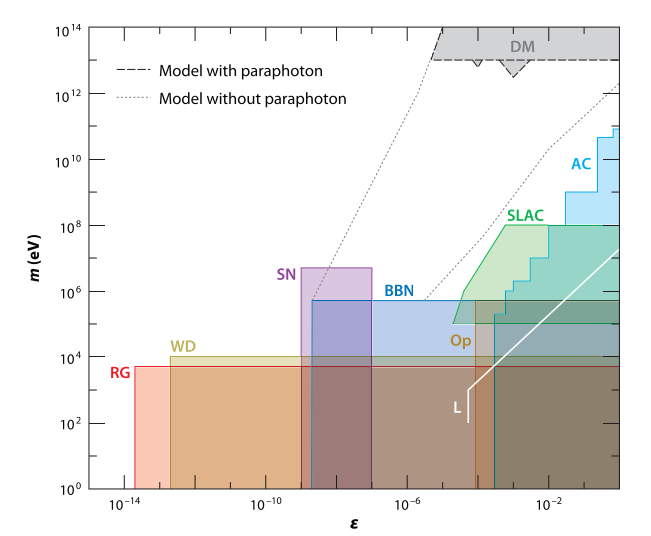
\includegraphics[width=0.8\textwidth]{figures/theory/lip_constraints.png}
\caption{Regions of mass-charge space ruled out for \acs{LIP}s from several different sources. The dashed line limits apply in the case of a dark sector photon (our case of interest), and the dotted line is the limit without dark photons. Abbreviations: AC, accelerator experiments; Op, search for the invisible decay of ortho-positronium; SLAC, the SLAC millicharged particle search; L, the Lamb shift; BBN, big bang nucleosynthesis; RG, plasmon decay in red giants; WD, plasmon decay in white dwarfs; DM, dark matter searches; SN, Supernova 1987A.  Figure from \cite{Perl2009}. }
\label{fig:lip_constraints}
\end{center}
\end{figure}

Unlike many of the constraints in Figure~\ref{fig:lip_constraints}, a search for fractionally charged cosmic rays is model independent. That is, it does not depend on the particular production mechanism of the \ac{LIP}, nor on its mass. A tacit assumption is made that the cosmic ray is high energy, and indeed such high energy \ac{LIP}s may be produced in the present era in violent astrophysical processes or between interaction of ordinary cosmic rays in the atmosphere \cite{Perl2009}. The analysis in Chapter~\ref{ch:lips} concerns the search for \ac{LIP} cosmic rays. The search sensitivity for \ac{LIP} cosmic ray searches is given in terms of flux, $\Phi$, with units cm$^{-2}$~sr$^{-1}$~s$^{-1}$ as a function of the ``charge fraction'' $f$, where $f$ is defined as the denominator of the \ac{LIP} fractional charge, $e/f$. See Figure~\ref{fig:lip_lims} for recent \ac{LIP} flux limits. 

\begin{figure}[htbp]
\begin{center}
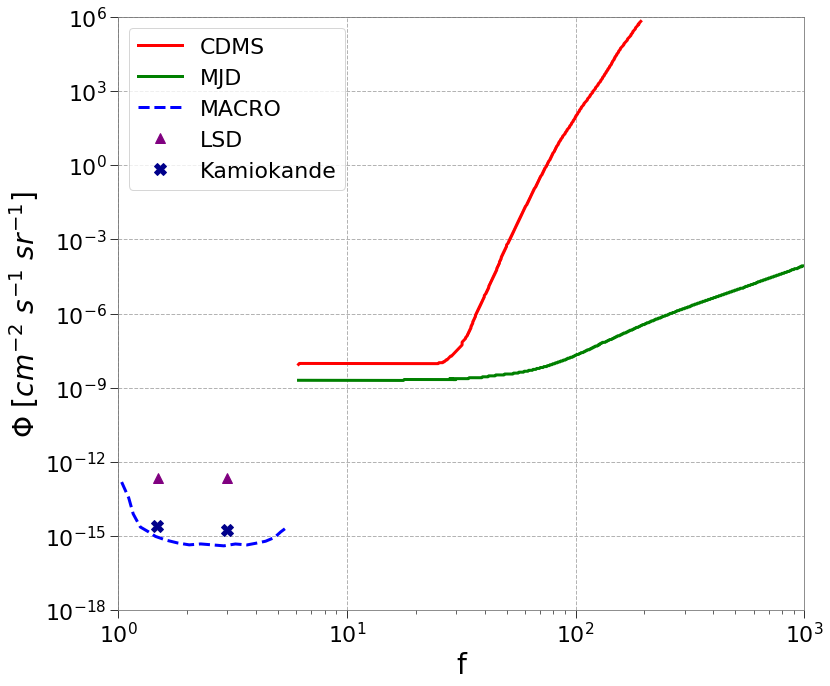
\includegraphics[width=0.8\textwidth]{figures/theory/lip_limits.png}
\caption{Recent limits on the flux of \acs{LIP}s with charge $e/f$ where $f$ is the x-axis. Figure reproduced from \cite{Alvis2018}. }
\label{fig:lip_lims}
\end{center}
\end{figure}


\subsection{WIMPless Miracle and the New Physics Flavor Problem}
As with any dark matter candidate, it is desirable for hidden sector dark matter to have the correct relic density. In Section~\ref{sec:wimp_miracle}, we discussed the \ac{WIMP} miracle: how a particle with a weak scale mass and coupling undergoes thermal freezeout to naturally produce the correct relic abundance. There is a similar situation for the hidden sector dubbed the ``\ac{WIMP}less miracle'', which is much more general. Recall that for a stable thermal relic particle $\chi$, the relic density $\Omega_{\chi}$ goes as:

\begin{equation}
\Omega_{\chi} \sim \langle \sigma_{A}v \rangle^{-1} \sim \frac{m_{\chi}^{2}}{g_{\chi}^{4}}
\end{equation}

The \ac{WIMP} miracle says that for $m_{\chi} \sim m_{weak}$ and $g_{\chi} \sim g_{weak}$, $\Omega_{\chi} \approx \Omega_{cdm}$. For a particle that interacts via a known \ac{SM} force, the weak force is the only reasonable choice, so $g_{\chi} \sim g_{weak}$. Hidden sector dark matter, however, has its own matter content and gauge forces, so many combinations of $(m_{\chi}, g_{\chi})$ are possible. This generalizes the \ac{WIMP} miracle to the \ac{WIMP}less miracle: hidden sector dark matter can produce the correct relic density, but need not have weak scale mass nor interact via the weak force (Figure~\ref{fig:wimpless_miracle}).

\begin{figure}[htbp]
\begin{center}
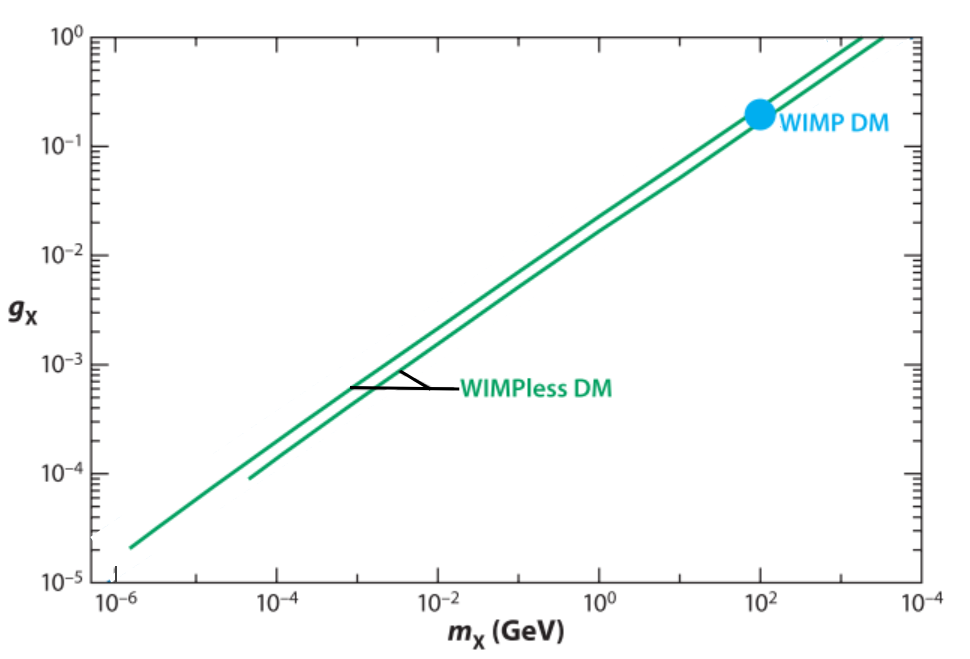
\includegraphics[width=0.8\textwidth]{figures/theory/wimpless_miracle.png}
\caption{Contours in the $(m_{\chi}, g_{\chi})$-plane for two different temperature conditions for the hidden sector. The upper line is for a hidden sector that achieves 80\% of the visible sector temperature after reheating, the lower line is for 30\%. For this plot, the hidden sector in assumed to be a 1-generation flavor-free version of the minimal supersymmetric standard model. Figure adapted from \cite{Feng2010}. }
\label{fig:wimpless_miracle}
\end{center}
\end{figure}

Recall also from Section~\ref{sec:wimp_miracle}, that in addition to it producing the correct relic abundance, the \ac{WIMP} is a favored dark matter candidate because it is related to \ac{SUSY}, which is introduced to solve the hierarchy problem of the \ac{SM}. In attempting to solve the gauge hierarchy problem, \ac{SUSY} gives rise to another problem called the ``new physics flavor problem'' \cite{Feng2010}. \ac{SUSY} particles may violate baryon number, lepton number, flavor, or CP. At the same time, we observe these symmetries to be extremely well preserved in the \ac{SM}. The new physics flavor problem, in a nutshell, is that not all \ac{SUSY} models are capable of elegantly conserving these symmetries. Creating models that solve the new physics flavor problem is a ``prime driver in the field of supersymmetric model building'' \cite{Feng2010}.  A particularly elegant subset of \ac{SUSY} models that do solve the new physics flavor problems are known as \ac{GMSB}. In these models, a hidden sector mediates \ac{SUSY} breaking\footnote{\ac{SUSY} is a symmetry that must be broken, otherwise a host of problems would be present. For example, without a broken \ac{SUSY}, the electron and selectron would have the same mass. Furthermore, selectrons are bosons. If we lived in a world where both electrons and selectrons were common, we would not have atomic structure because orbital fermionic electrons are a higher energy state than infinite ground state selectrons.}. In \ac{WIMP}less scenarios, one asks why the hidden sector dark matter should be stable. For \ac{GMSB} models, which solve the new physics flavor problem, an elegant way to stabilize the hidden sector dark matter is through the hidden U(1) charge conservation, which necessitates a massless gauge boson in the hidden sector. This is precisely the situation we have with \ac{LIP}s. To quote \cite{Feng2010}: ``In summary, hidden sector dark matter models may in fact be motivated by leading problems in particle physics, and may even have naturally the correct relic density, through a generalization of the \ac{WIMP} miracle to the \ac{WIMP}less miracle.''

\subsection{Charge Quantization}
It is known experimentally that all charged particles in the \ac{SM} have charge $\pm\frac{1}{3}e$, $\pm\frac{2}{3}e$, or $\pm e$. However, there is no theoretical motivation behind this quantization of electric charge. Holdom suggested a new, U(1) with a ``paraphoton'' gauge boson could produce quantized charge in the \ac{SM} and transfer fractional shifts to fermions that interact with the paraphoton \cite{Holdom1986}, which is the \ac{LIP} paradigm. Others, \cite{Foot1993}, \cite{Babu1990}, \cite{Schellekens1990}, \cite{Wen1985}, and \cite{Dirac1931}, have proposed various extensions to the \ac{SM} that would produce charge quantization. Some of these theories yield fractionally charged particles, and all of them require new physics beyond the \ac{SM}. It is useful to note that even outside of the hidden sector, there are theoretical motivations for fractionally charged particles. 


\section{Experimental Strategies for Detecting Dark Matter}
\label{sec:dm_detection_schemes}
Experiments designed to detect dark matter, be it \ac{WIMP}, axion, dark sector, or other candidates, fall into three main categories: production, indirect detection, and direct detection (see Figure~\ref{fig:dm_detection_schemes}). Detection schemes and examples are discussed in the following subsections. All three methods are in use to provide a diverse, multipronged \ac{DM} detection program. 

\begin{figure}[htbp]
\begin{center}
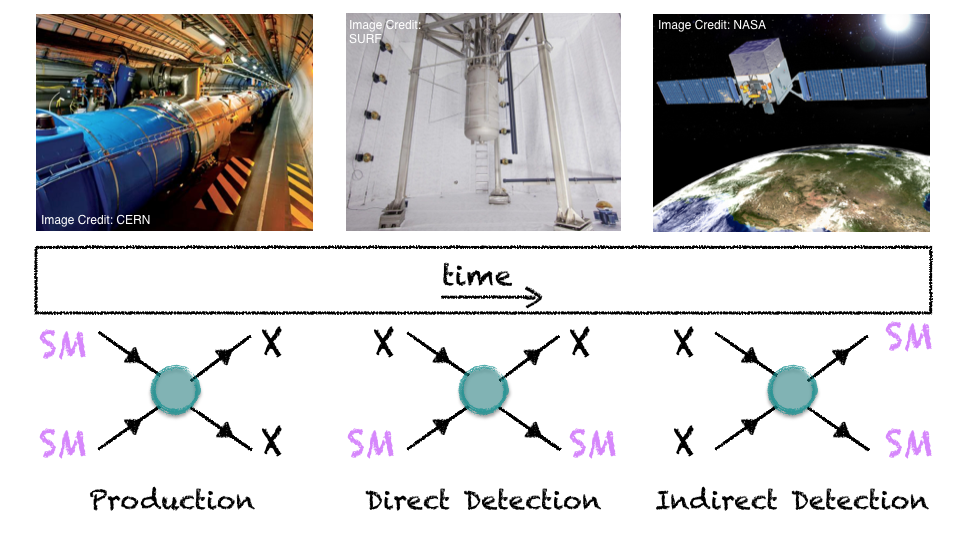
\includegraphics[width=\textwidth]{figures/theory/dm_detection_schemes.png}
\caption{Summary of \acs{DM} detection schemes with illustrative Feynman diagrams. In all cases, the arrow of time is from left to right. (left) \acs{SM} particles can be collided at high energy facilities, which may produce \acs{DM} particles, $\chi$. (center) $\chi$ may scatter with \acs{SM} particles, leaving behind a characteristic signal. (right) $\chi$ particles in the galaxy may annihilate and produce \acs{SM} particles, which produces an \acs{SM} signal in excess of expectations from standard astrophysical processes.}
\label{fig:dm_detection_schemes}
\end{center}
\end{figure}

\subsection{Production}
Colliders like the \ac{LHC} are capable of accelerating \ac{SM} particles to high energies. The \ac{SM} particles, typically protons, antiprotons, electrons, and/or positrons, can be collided with each other or with a fixed target. In general, dark matter produced in these collisions appears as ``missing energy'' when the event is reconstructed. If a multitude of events is missing the same amount energy $E$, that is a classic indication that there is a new particle with mass $m = E/c^{2}$. A recent overview of collider searches for several different dark matter candidates can be found in \cite{Penning2018}. 

\subsubsection{LIP Production}
It is noted in \cite{Perl2009} that ``high-energy electron-positron colliders provide the most definitive search method among accelerator and collider searches for fractionally charge particles [in the range $\pm\frac{1}{3}e -\pm \frac{4}{3}e$].'' This is due to the production cross section being large and known to high accuracy. Another successful collider method to search for fractionally charged particles with charge $<<1$ is a ```beam dump''. In beam dump experiments, the collider accelerates e.g. an electron into a fixed target, producing secondary particles. A large mass of shielding is between the target and the detector. Only secondary particles with a small charge can make it through the shielding to reach the detector. The limit in Figure~\ref{fig:lip_constraints} titled SLAC is from a beam dump type experiment; see \cite{Prinz1998} for details about the SLAC millicharged particle search.

\subsection{Indirect Detection}
The signal of dark matter annihilation can appear in both ground-based and satellite detectors. Dark matter may decay or annihilate into \ac{SM} particles, which can be detected by conventional detectors. Positive identification of an indirect dark matter signal is difficult due to large potential backgrounds from astrophysical sources, which are not perfectly understood. However, indirect detection can probe questions collider and direct searches cannot, such as whether \ac{DM} is perfectly stable and what the annihilation cross sections are. 

\subsubsection{LIP Indirect Detection}
Indirect limits for fractionally charged particles come from stellar evolution and supernovae (see limits titled WD, RG, and SN in Figure~\ref{fig:lip_constraints}). Essentially, new low-mass particles can be produced in the hot and dense medium of stars, and eventually escape, carrying away energy \cite{Davidson2000}. The additional energy-loss channel modifies stellar evolution, and observations of brightness, etc. can set a limit on the \ac{LIP} mass and interaction strength. For Supernova 1987A, the number of neutrinos detected at Earth roughly agrees with theoretical expectations. If fractionally charged particles contribute to cooling, the neutrino flux would decrease; the SN limit in Figure~\ref{fig:lip_constraints} is from such an analysis \cite{Perl2009} \cite{Davidson2000}.

\subsection{Direct Detection}
In direct detection, experimentalists seek to observe \ac{DM} interactions in a detector composed of \ac{SM} materials. Detectors are designed with a \ac{DM} candidate in mind, and aspects of the detector are optimized at the design stage to search for one type of \ac{DM}. Because direct detection searches are built with a particular \ac{DM} candidate in mind, backgrounds can be controlled and minimized much more than in indirect or production searches. Of course, a given detector can search for \ac{DM} candidate even if it was not initially designed to do so, and in this case, the search still benefits from the detailed understanding of backgrounds in the detector. Most current direct detection programs fall into one of two categories: \ac{WIMP} detector or axion detector. In the case of \ac{WIMP} detectors, the detector target material is some homogenous material like solid Ge or liquid Xe, and experimentalists seek to detect energy deposition consistent with that of a \ac{WIMP} causing a nuclear recoil in the target. This type of detector must be composed of radiopure materials and located deep underground to be capable of detecting rare \ac{WIMP} interactions. In the case of axions, the detector is a resonator cavity with a strong magnetic field, which couples with the axion field. Cosmic rays and radioactivity are not backgrounds for axion detection, so these detectors need not be placed underground or built of radiopure materials; however, their electronic noise must be strictly managed. Axion detectors take advantage of a resonance amplification of their signal that would occur at a specific axion mass and coupling. To observe the resonance signal, detector background noise must be kept sufficiently low. 

\subsubsection{LIP Direct Detection}
Direct detection searches for fractionally charged particles include schemes like the Millikan drop experiment, which modern methods have improved upon (see \cite{Perl2009} for more detail). Table-top style experiments searching for the decay of ortho-positronium, or changes in the Lamb shift, would indicate additional couplings to a hidden sector \cite{Perl2009}; these are marked Op and L in Figure~\ref{fig:lip_constraints}, respectively. Large water or liquid scintillator detectors such as Kamiokande and MACRO performed searches for fractionally charged cosmic rays from $e$ down to $e/6$ (see Figure~\ref{fig:lip_lims}). More recent searches from \ac{CDMS} and \ac{MJD} extend the charge fraction range of these searches down to $\sim e/1000$. These last two searches are both from cryogenic Ge detectors designed with other goals in mind -- \ac{CDMS} is a canonical \ac{WIMP} detector and \ac{MJD} is a neutrinoless double beta decay experiment. A similar search for cosmic ray \ac{LIP}s is carried out in Chapter~\ref{ch:lips} with the \ac{LUX} experiment, which is also a canonical \ac{WIMP} detector, but uses \ac{LXe} for its target material. More details about \ac{LXe} as a detector medium are found in Chapter~\ref{ch:LXeTPCs}. Details about the \ac{LUX} detector can be found in Chapter~\ref{ch:LUX}.



%*****************************************
%*****************************************
%*****************************************
%*****************************************
%*****************************************

%************************************************
\chapter{Particle Detection with Liquid Xenon}

\label{ch:LXeTPCs} 
%************************************************

\section{Liquid Xenon as a Detector Medium}
Liquid xenon detectors are powerful tools for rare event searches. In particular, the dual phase \ac{LXe} \ac{TPC} has been very successful in accessing \ac{WIMP} parameter space and currently holds the worlds most sensitive limits on \ac{WIMP}s. This section describes the properties of \ac{LXe} and the basic principles of \ac{TPC}s that have allowed this technology to play a large role in the hunt for dark matter.

\subsection{Properties of Liquid Xenon}
Liquid xenon has many properties relevant to particle detection, particle identification, and also many properties related to the ease of detector operation:

\begin{itemize}
  \item The density of \ac{LXe} is 2.9~g/cm$^{3}$ at 170~K, much denser than other possible \ac{TPC} target materials, such as liquid argon which has density 1.4~g/cm$^{3}$ at 87~K. The advantage in this two-fold: (1) the same volume contains more kg of Xe than Ar, so for two detectors of the same volume, one filled with Xe and the other with Ar, both running for one year, the Xe detector has more exposure; (2) xenon's high density effectively stops external radiation, producing an ultra-low-background volume in the center of the detector where rare-event searches can be performed (this region is called the ``fiducial volume'').
  
  \item Xenon gas is easily liquefied with liquid nitrogen (77~K) or commercially available pulse tube refrigerators.

  \item Xenon has no long-lived radioisotopes that cause troublesome backgrounds. The one exception is the 2$\nu\beta\beta$ decay of $^{136}$Xe (natural abundance 8.875\%) with measured half-life of $2.1 \times 10^{21}$ years. The long half-life and relatively low abundance together result in a very low count rate, and the isotope can be used to search for neutrino-less double beta decay ($0\nu\beta\beta$).
  
  \item Xenon, as a noble element, is easily purified with a heated getter to rid electronegative impurities. Some of these impurities absorb xenon scintillation light, e.g. N$_{2}$, and others can attract electrons, interferring with the ionization signal in \ac{TPC}s, e.g. O$_{2}$.
  
  \item The comparatively large mass of xenon allows it to be purified of other noble gasses via gas chromatography \cite{LUXKrRemoval2018} and cryogenic distillation \cite{Xe1TKrRemoval2017}. As other noble gasses cannot be removed via getter, this feature is extremely useful in removing the troublesome background of $^{85}$Kr decay. $^{85}$Kr decays via beta emission to stable $^{85}$Rb with a half-life of 10.8 years and Q$_{\beta}$ = 687~keV. The decay proceeds directly to the $^{85}$Rb ground state with a branching ratio of 99.6\%. Since no de-excitation of $^{85}$Rb follows, this beta decay cannot be rejected as background by coincidence with a gamma, and relies purely on the ability to discriminate between WIMP-like \ac{NR} and beta- or gamma- produced \ac{ER}. While ER/NR discrimination is one of the features of \ac{LXe} \ac{TPC}s (described in Section~\ref{sec:er_nr_discrimination}), leakage of \ac{ER} events in to the \ac{NR} signal region can occur and the best mitigation is to remove as much of the  $^{85}$Kr as possible. Single-phase \ac{LXe} detectors, with no ER/NR discrimination, benefit greatly from the ability to remove $^{85}$Kr.
  
  \item Particles interacting in \ac{LXe} excite atoms and create electron ion-pairs, producing detectable quanta: scintillation photons and ionization electrons, respectively (described in section \ref{sec:signal_generation}).
  
  \item Xenon produces scintillation light of wavelength $\lambda$~=~178~nm (described in Section~\ref{sec:signal_generation}). Xenon is transparent to this wavelength so it can propagate freely and be directly detected with current \ac{PMT} technology, and doesn't require the use of e.g wavelength shifter. 
  
  \item Ionization electrons produced in particle interactions can be drifted and extracted into a gaseous region via applied electric fields, where they undergo proportional scintillation. By this method, a single electron is amplified many-fold into detectable photons. This basic operating principle of dual-phase \ac{TPC}s makes even a single ionization electron detectable. 
  
  \item Xenon has high light and charge yields, and therefore a low threshold for producing detectable quanta. A useful quantity is the so-called `W-value' of \ac{LXe}: W = 13.7 $\pm$ 0.2 eV \cite{Dahl2009}. The W-value, analogous to a work-function, is a measure of the average energy expenditure to produce one quanta (scintillation photon or an ionization electron) from liquid xenon. 
  
  \item \ac{LXe} \ac{TPC}s are easily scalable: creating a large homogenous volume is straightforward. In contrast, solid state detectors, such as cryogenic Ge, are more difficult to scale up directly and require instead the production of multiple small modules (O(10)~cm) which each must be instrumented separately.  
    
\end{itemize}


\subsection{Scintillation and Ionization Signal Generation}
\label{sec:signal_generation}
A particle can interact with a xenon atom through interaction with an orbiting electron, creating an \ac{ER}, or though an interaction with the xenon nucleus, where the nucleus is imparted with momentum and recoils, \ac{NR}. Some energy is lost to atomic motion (heat). The recoiling electron or nucleus loses energy via interaction with neighboring xenon atoms, creating more excited atoms and electron-ion pairs. The excited xenon atoms, Xe$^{*}$, combine with other atoms to form an excited dimer, or excitons, Xe$_{2}^{*}$. The excited dimer forms two states: a triplet and a singlet, which de-excite with the emission of a 178~nm photon. The lifetimes of the triplet and singlet are measured to be 24~ns and 3~ns, respectively \cite{Mock2014}. Since the scintillation light is produced by the excimer, which has a different electronic structure than atomic xenon, the light is free to propagate through the detector and will not be absorbed by the atomic xenon. The Xe$^{+}$ ions of the electron-ion pairs combine with other Xe atoms to form dimers Xe$_{2}^{+}$, and these dimers can combine with electrons (from the electron-ion pairs) to form excitons, Xe$_{2}^{*}$, which then decay and produce additional 178~nm scintillation photons. This process is called recombination. If no electric field is applied, all electron-ion pairs recombine to produce additional scintillation photons. If an external electric field is present, some electrons can be drifted away from the interaction site to be detected with other methods. 

The sensitivity of liquid xenon detectors to low energy recoils depends on their ability to detect the 178~nm scintillation photons with high-efficiency. High \ac{QE} \ac{PMT}s constructed with ultra-low radioactivity materials are the go-to instrument for this purpose. In addition to high-efficiency photon-detectors, liquid xenon detectors must also have high geometrical light collection efficiency to optimize sensitivity. Single-phase liquid xenon detectors, where no electric field is applied, maximize light-collection by with a spherical geometry, endeavoring to cover 4$\pi$ steradians surrounding the \ac{LXe}. The XMASS detector uses spherical geometry to accomplish photocathode coverage of \~62\%, and two types of Hamamatsu \ac{PMT}s (R10789-11 and R10789-11MOD) with \ac{QE} of 28\%, and quote a signal collection efficiency of 20\% \cite{Abe2013}, \cite{XMASSCollaboration2018}. Dual-phase \ac{TPC} detectors are lined with \ac{PTFE} to take advantage of its extremely high (~99\%) reflectivity for 178~nm light in \ac{LXe} \cite{Neves2017}. The \ac{LUX} detector uses a cylindrical geometry, with all non-light-collectiing surfaces lined with \ac{PTFE}, and Hamamatsu R8778 \ac{PMT}s (\ac{QE} of 33\%) only on the top and bottom of the detector (low photocathode coverage), to accomplish a light collection efficiency of 90\% \cite{Faham2014a}.

If the detector is a \ac{TPC} the ionization electrons are drifted away from the interaction site to be detected. Single phase \ac{TPC} employ thin wires to collect the ionization electrons. For example, the EXO-200 experiment is a single-phase liquid xenon \ac{TPC} that uses crossed-wire planes to collect the ionization electrons and avalanche photodiodes to collect the scintillation photons \cite{Auger2012}. \ac{LUX} is a dual-phase xenon \ac{TPC}, where ionization electrons produced in the large liquid region are drifted and extracted into gaseous xenon via applied electric fields, where they undergo proportional scintillation. The proportional scintillation light is the same 178~nm wavelength as scintillation in the liquid produced in the liquid, and it is similarly collected via high \ac{QE} \ac{PMT}s.

In addition to light-collection efficiency, the sensitivity of \ac{TPC} xenon detectors also depends on their ability to collect signal from the ionization electrons. There are challenges in delivering \ac{HV} to liquid xenon in order to set up the electric field which drifts the ionization electrons (some of these challenges are explained in Chapter \ref{ch:testbed}). Additionally, electronegative impurities such as oxygen (O$_{2}$) present in the detector attract and capture ionization electrons as they drift, eating away the ionization signal. These non-noble impurities are removed by constantly circulating the xenon through a heated zirconium getter and returning it to the detection volume. Purification through a getter must be done in gaseous phase, so liquid xenon removed from the detection volume is evaporated, passed through the getter via a circulation system, and re-condensed into the detection volume. 


\section{Dual-Phase Xenon Time Projection Chamber}
A particle interacting in a noble liquid or gas target deposits energy into scintillation and ionization channels (Section \ref{sec:signal_generation}). The basic operating principle of \ac{TPC}s is to drift the ionization electrons away from the interaction site and detect them at a later time than the scintillation signal is detected. A dual phase liquid xenon \ac{TPC} is a type of \ac{TPC} with a large liquid target volume and a small region of xenon vapor above the liquid volume, instrumented with light sensors (typically \ac{PMT}s). A particle interacting in the liquid target produces both scintillation photons and ionization electrons at the interaction site. The scintillation photons are promptly detected by the \ac{PMT}s, this primary signal is called S1. The ionization electrons are drifted upward to the gas region by an applied electric field, and extracted across the liquid-gas boundary by a higher electric field, where they undergo proportional scintillation and produce a second signal detected by the \ac{PMT}s, called S2. The field is supplied by a series of electrodes, composed of wire planes, grids, or chemically etched meshes, held at constant voltages. The bottom-most field-producing electrode is called the cathode, at the top of the liquid region is the gate or extraction electrode, followed O(1)~cm by the anode. The liquid region is often referred to as the `drift region' and region between the gate and anode is referred to as the `extraction region'. The drift region takes up by far more volume than the extraction region. The electrons are extracted from liquid to gas with some efficiency, called the \ac{EEE}. This efficiency plays an important role in the operation of dual-phase \ac{LXe} \ac{TPC}s, and is discussed further in  \textbf{E-Train CHAPTER}.

The S2 in a dual-phase \ac{TPC} plays two important roles: (i) internal amplification of the signal, whereby a few electrons are transformed into O(10) times as many photons (ii) $(x,y)$ localization via \ac{PMT} hit pattern. The time spacing of the S1 and S2 signals can be converted to depth ($z$) of the interaction, providing full $(x,y,z)$-reconstruction of the interaction position.

\begin{figure}[htbp]
\begin{center}
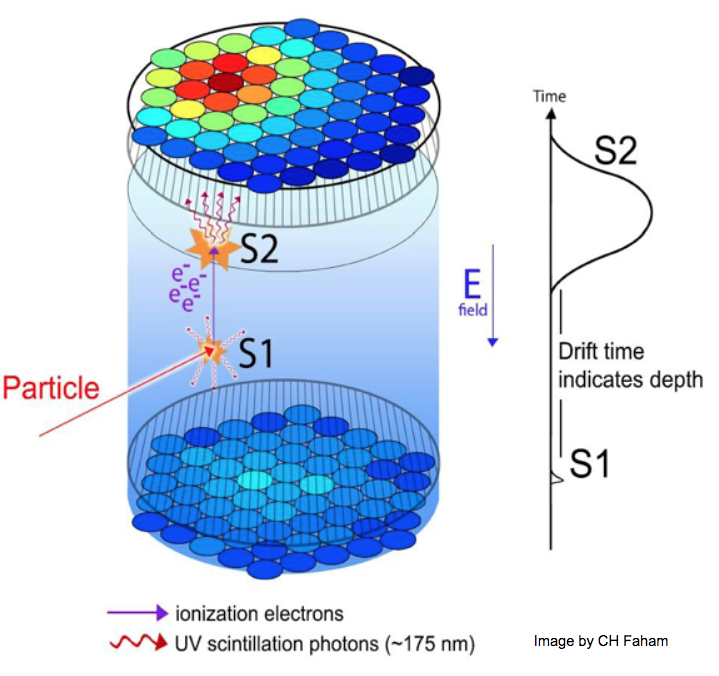
\includegraphics[width=\halffig]{figures/lxetpcs/TPC.png}
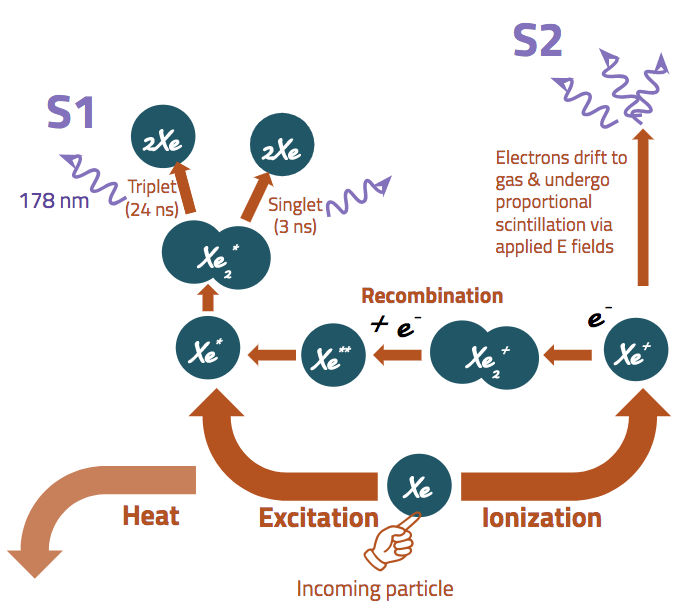
\includegraphics[width=\halffig]{figures/lxetpcs/signal_generation_in_lxe_tpcs.png}
\caption{ (left) Diagram of a dual-phase xenon time projection chamber. The time difference between S1 and S2 gives the depth ($z$) of the interaction, and $(x,y)$ is reconstructed from the S2 signal. (right) Diagram summarizing the generation of the scintillation and ionization signal generation in dual-phase xenon time projection chambers.}
\label{fig:tpc}
\end{center}
\end{figure}



\subsection{Energy Reconstruction}
\label{sec:energy_reconstruction}
Energy reconstruction in dual-phase xenon \ac{TPC}s comes from the measurable quantities, S1 and S2, but begins with the number of excitons $n_{ex}$  and electron-ions pairs $n_{i}$ generated at the interaction site. 
\begin{equation}
E = f W (n_{ex} + n_{i} )
\end{equation}

where $E$ is the deposited energy. $W$ is the average energy needed to produce a single excited or ionized atom, $W = 13.7 \pm 0.2$~eV \cite{Mock2014}. The quenching factor, $f$ is 1 for electronic recoils but $f \neq 1$ for nuclear recoils. For now, take the case of electronic recoils and set $f=1$. This equation can be rewritten:

\begin{equation}
E_{ER} = W (1 + \frac{n_{ex}}{n_{i}} ) n_{i}
\end{equation}

The ratio of excitons to ions is constant for electron recoils $n_{ex}/{n_{i}} = 0.2$ \cite{LUX:YieldsAndRecombination}. As discussed in Section \ref{sec:signal_generation}, each exciton deexcites, emitting a 178~nm photon, some fraction $r$ of the initial electron-ion pairs recombine and form additional excitons. The total number of prompt scintillation photons created by the interaction is then:

\begin{equation}
n_{\gamma} = (r + \frac{n_{ex}}{n_{i}} ) n_{i}
\end{equation}

And the total number of electrons created by interaction site (electrons escaping recombination) is:

\begin{equation}
n_{e} = (1 - r ) n_{i}
\end{equation}

Thus, the effect of recombination is to ``trade-out'' electrons for photons, but the total number of quanta is conserved (Figure~\ref{fig:recombination} (left)). The amount of recombination depends on applied electric field, \ac{LXe} density, and particle energy \cite{LUX:YieldsAndRecombination}. In the case of the 122~keV electron recoils in Figure~\ref{fig:recombination} (right): at low fields, most of the electron-ion pairs recombine, which results in more scintillation photons. As the applied electric field increases, more electrons are pulled away from the interaction site resulting in fewer scintillation photons and more ionization electrons. These amounts of photons and electrons are referred to as the scintillation and ionization yields. The two quantities, $n_{\gamma}$  and $n_{e}$ relate directly to the observable S1 and S2 signals:

\begin{equation}
\label{eq:energy}
\begin{split}
E_{ER} &= W (n_{\gamma} + n_{e} ) \\
   &= W (\frac{S1}{g_{1}} + \frac{S2}{g_{2}})
\end{split}
\end{equation}

where $E_{ER}$ reminds us that we are taking the case of electronic recoils and set $f=1$ in Equation~\ref{eq:energy}. S1 and S2 are in units of detected photons (phd) or photoelectrons (phe), and $g_{1}$ and $g_{2}$ are detector gains in units of phd / quanta or phe / quanta\footnote{An distinction should be made between the traditional units of phe and the units of phd which are used in many LUX publications. The Hamamatsu R8778 PMTs used in LUX emit two photoelectrons for a single VUV photon \~20\% of the time \cite{Faham2015}, but the PMT gain calibration photons (from blue LEDs) do not. LUX performed additional calibration with VUV photons to account for the difference, and report detected photons instead of photoelectrons \cite{LUX:Run03Comprehensive}}. $g_{1}$ is the detection efficiency for the prompt scintillation photons: it is a product of the the average a geometrical light collection efficiency and the average \ac{PMT} \ac{QE}. Typical values for $g_{1}$ are in the range of 0.01-0.02. $g_{2}$ is the analogous quantity for S2 proportional scintillation light: it is a product of the \ac{EEE} and the average number of detected photons produced by one extracted electron. Typical values for $g_{2}$ are in the range 10-60.



\begin{figure}[htbp]
\begin{center}
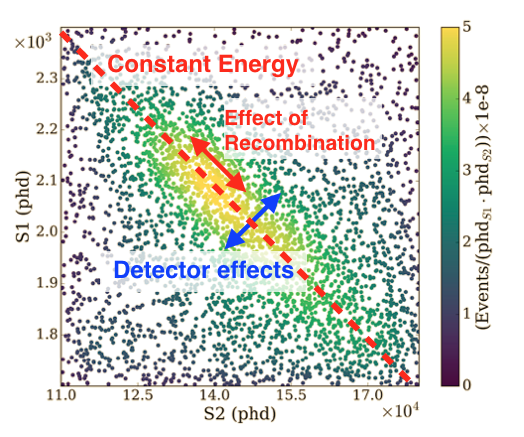
\includegraphics[width=\halffig]{figures/lxetpcs/recombination.png}
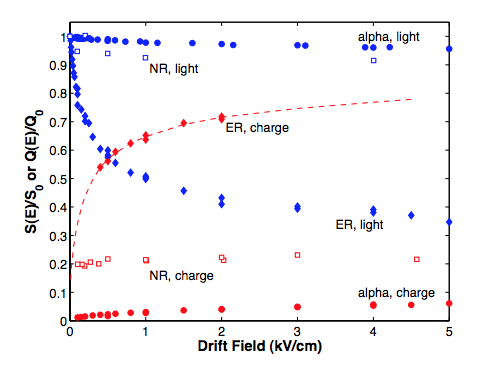
\includegraphics[width=\halffig]{figures/lxetpcs/yields.png}
\caption{(left) Plot illustrating the effect of recombination and detector effects on a line source (127Xe), courtesy of E. Pease. (right) Field dependence of scintillation and ionization yield in LXe for 122 keV electron recoils (ER), 56.5 keVr nuclear recoils (NR) and 5.5 MeV alphas, relative to the yield with no drift field from \cite{Aprile2010}}
\label{fig:recombination}
\end{center}
\end{figure}

To properly reconstruct the energy of nuclear recoils, we must revisit the quenching factor factor $f$. Equation~\ref{eq:energy} then becomes:

 \begin{equation}
 \begin{split}
E_{NR} &= f W (n_{\gamma} + n_{e} ) \\
   &= f W (\frac{S1}{g_{1}} + \frac{S2}{g_{2}})
 \end{split}
\end{equation}

This equation can be rewritten:

 \begin{equation}
 \label{eq:combined_energy}
E_{NR} = f E_{ER} = \frac{E_{ER}}{\mathcal{L}}
\end{equation}

where $\mathcal{L}$ is Lindhard's factor. Lindhard's factor accounts for the fraction of energy lost to atomic motion (heat) in nuclear recoils \cite{Lindhard1963}. An incoming particle interacts with a ``patient zero'' Xe atom, resulting a nuclear recoil. The patient zero Xe atom interacts with surrounding atoms in a cascade to produce S1 and S2; it is the energy partitioning in this cascade that results in different energy scales for \ac{ER} and \ac{NR}. Lindhard shows that the energy partitioned in nuclear interactions and electron interactions from a recoiling xenon nucleus is:

 \begin{equation}
 \label{eq:lindhard}
\mathcal{L} = \frac{k g(\epsilon)}{1 + k g(\epsilon)}
\end{equation}

where $k = 0.133 Z^{2/3} A^{-1/2}$ is a proportionality constant that relates electronic stopping power and the velocity of the recoiling xenon atom, and $\epsilon = 11.5 (E_{NR}/keV) Z^{-7/3}$. Lindhard's calculation yields $k=0.166$, which is the commonly accepted value. Measurements of nuclear recoils in \ac{LXe} are used to fit for $k$. Several experiments were compared by Sorensen and Dahl to determine that nuclear recoil energy is well described by $0.110 < k < 0.166$ \cite{Sorensen2011}. Results from \ac{LUX} yielded $k = 0.1735 \pm 0.0060$ \cite{LUXDD}. 


If it is not known \textit{a priori} whether an interaction is a nuclear recoil or electron recoil, the `electron equivalent' energy is given in units $keV_{ee}$. If it is known that the recoil is a nuclear recoil, Lindhard's factor is applied and the units can be given in $keV_{nr}$. Lindhard's factor allows us to combine nuclear recoils and electronic recoils on one energy scale by labelling contours of constant reconstructed energy with both $keV_{ee}$ and $keV_{nr}$ (example in Figure~\ref{fig:e_contours}).


\begin{figure}[htbp]
\begin{center}
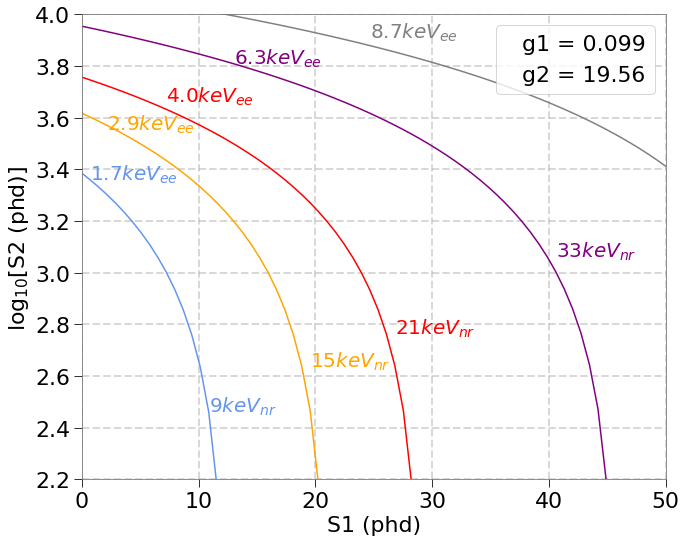
\includegraphics[width=\halffig]{figures/lxetpcs/E_contours.png}
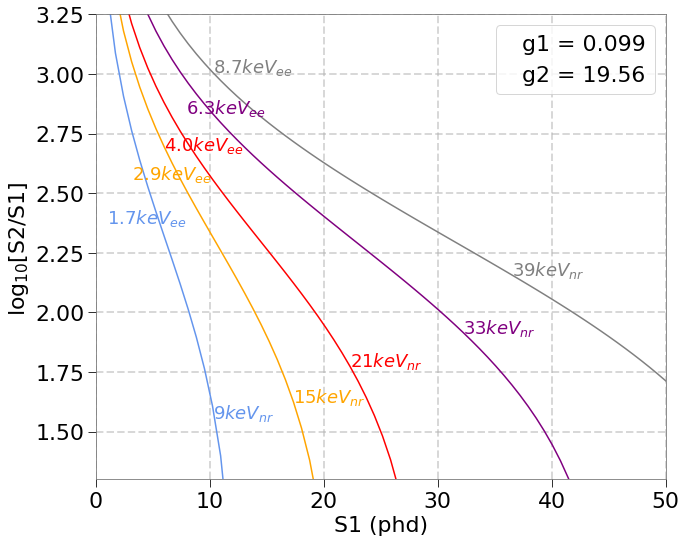
\includegraphics[width=\halffig]{figures/lxetpcs/E_contours2.png}
\caption{Plots showing combined energy contours in two common sets of axis units, for an example set of $g_{1}$ and $g_{2}$.}
\label{fig:e_contours}
\end{center}
\end{figure}



\section{Dual-Phase Xenon TPCs for Dark Matter Detection}
Dual phase Xe \ac{TPC}s have been at the forefront of the hunt for dark matter in the last several decades. As described above, the xenon medium and detector technology make excellent low-background, rare-event searches with high signal yields. Dual phase Xe \ac{TPC}s also provide a few enhancements to WIMP dark matter searches, but other dark matter or rare event searches are also possible with the same detector.


\subsection{WIMP Searches with LXe TPCs}
Dual-phase \ac{LXe} \ac{TPC}s are optimized for WIMP searches. They have been very successful in reaching large areas of WIMP parameter space. 

\subsubsection{ER, NR Discrimination}
\label{sec:er_nr_discrimination}
One of the most powerful features of \ac{LXe} \ac{TPC}s, which has made the technology especially useful in the hunt for WIMP dark matter, is the ability to discriminate between electron recoils and nuclear recoils. \ac{WIMP} interactions are expected to be nuclear recoils, but most natural radioactivity ($\beta , \gamma$) are electron recoils. The amount of recombination for equal energy \ac{ER} and \ac{NR} is different, so for events with the same reconstructed energy $E$(keV$_{ee}$), the ratio of S2/S1 is characteristically different. A useful discrimination space is log$_{10}$(S2/S1) vs S1, as the distributions of log$_{10}$(S2/S1) for \ac{ER} and \ac{NR} events are Gaussian. Different calibration sources are used to develop a population of events known to be \ac{ER} and a population of events known to be \ac{NR}, these calibration sources reveal what is known as the \ac{ER} and \ac{NR} bands (Figure~\ref{fig:bands}).

\begin{figure}[htbp]
\begin{center}
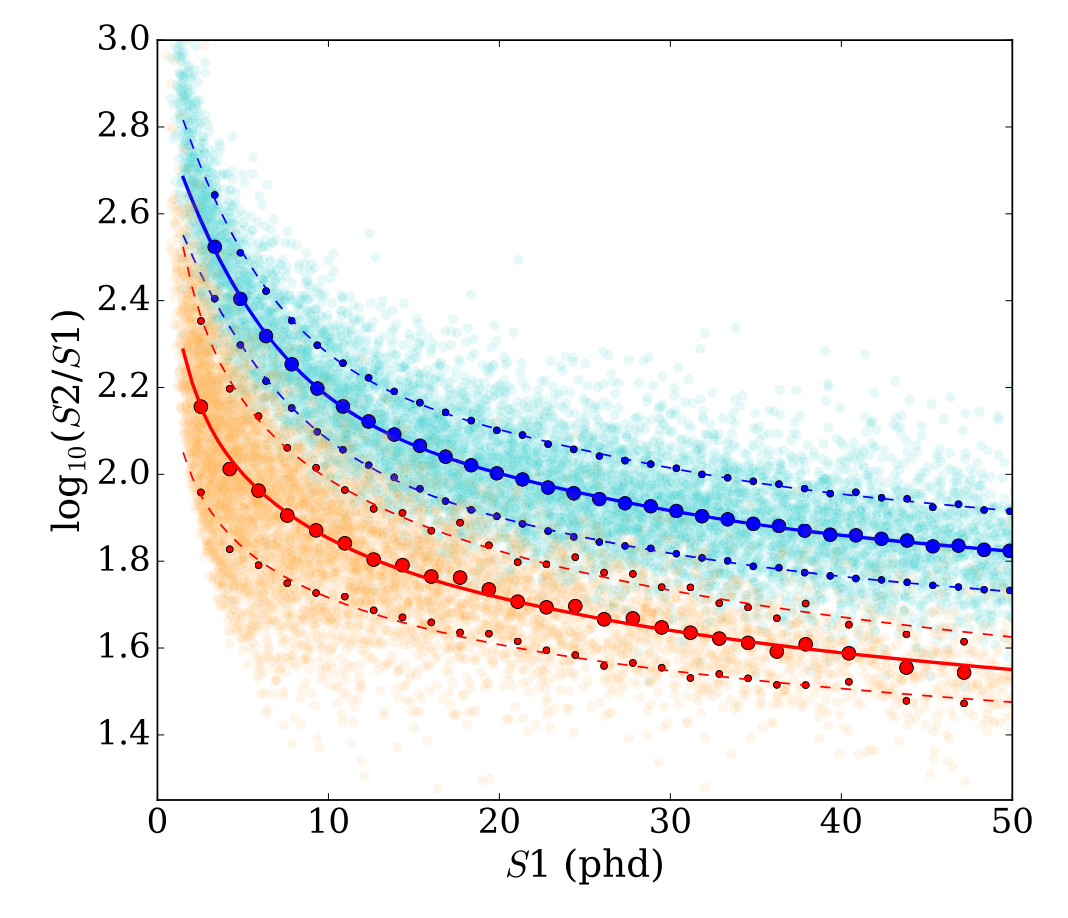
\includegraphics[width=0.65\textwidth]{figures/lxetpcs/bands.png}
\caption{Plot showing ER and NR bands from LUX. Solid lines are the ER and NR Gaussian means $\mu$, dotted lines are $\mu \pm 1 \sigma$. Figure from \cite{LUX:YieldsAndRecombination} }
\label{fig:bands}
\end{center}
\end{figure}


In the course of a \ac{WIMP} search, the experimentalists are tasked with keeping a stable detector operating for months or years. In this time, the detector will see events of natural radioactivity and perhaps \ac{WIMP}s. The natural radioactivity appears in the \ac{ER} band (location of bands is known from calibration), and nuclear recoil events appear in the \ac{NR} band. Due to band overlap, only events appearing below the \ac{NR} mean are considered \ac{WIMP} candidates. This restriction cuts signal acceptance to 50\%, but allows dual-phase \ac{TPC}s to reject background electronic recoils at $\gtrsim$99\%. The background acceptance rate is known as \ac{ER} leakage. It is the fraction of events appearing below the \ac{NR} mean from the \ac{ER} calibration source. For a background rejection rate of 99.99\%, the \ac{ER} leakage is 0.01\%, this number determines the sensitivity of the detector.


\subsubsection{WIMP Rates and Cross Section}
\label{sec:wimp_rates}
The choice of direct detection for \ac{WIMP} searches was touched on in Section~\ref{sec:dm_detection_schemes:}. Here, we go through the specifics of \ac{WIMP} rates and their cross section in \ac{LXe}, showing that the \ac{LXe} \ac{TPC} technology gets an enhancement that makes it especially suited for \ac{WIMP} searches.

\ac{WIMP}s scattering in the \ac{TPC} produce measurable nuclear recoils. The shape of this nuclear recoil spectrum determines eventually the number of \ac{WIMP} events observed, and it depends on both \ac{WIMP} properties and detector properties. The energy imparted to nucleus depends on \ac{WIMP} mass $M_{\chi}$ and velocity distribution, as well as the mass of the target nucleus $M_{T}$ and a nuclear form factor $F$ that governs how effectively energy is transferred to the nucleus. Assuming a uniform, spherical dark matter halo, estimates for the local density of dark matter $\rho{\chi}$ can be made from astrophysical observations. The velocity distribution $f(v)$ is assumed to be isotropic and Maxwellian, with a cut-off at the escape velocity $v_{esc}$ of the Milky Way. If we account for the velocity of the Earth through the galactic plane $v_{E}$, the velocity distribution is shifted: $f(v) = f(v,v_{E})$. Following Lewin and Smith \cite{Lewin1996}, we can write the local number density:


\begin{equation}
\begin{split}
dn &= \frac{n_{0}}{k} f(v, v_{E}) d^{3}v \\
     &= \frac{n_{0}}{k} exp \big( - \frac{(v + v_{E})^{2} }{ v_{0}^{2}} \big) d^{3}v 
\end{split}
\end{equation}

Where $n_{0} = p_{\chi}/M_{\chi}$ is the average local number density of dark matter particles, $v_{0} \approx~220km/s$ \cite{?} is the mean of the dark matter velocity distribution, and $k$ is a normalization constant such that $\int_{0}^{v_{esc}} \equiv n_{0}$. If the escape velocity is infinite, the normalization integral is easily evaluated:

\begin{equation}
k = \int_{0}^{2\pi} \int_{-1}^{1i} d(cos\theta)  \int_{0}^{\infty} f(v, v_{E}) v^{2}dv = (\pi v_{0}^{2})^{3/2} \equiv k_{0}
\end{equation}

$v_{esc}$ is not infinite ($v_{esc} \approx 544~km/s$ \cite{Baudis2014}), and so the normalization integral evaluates to:

\begin{equation}
k =  k_{0} \Big[ erf\big(\frac{v_{esc}}{v_{0}}\big) - \frac{2}{\pi^{1/2}} \frac{v_{esc}}{v_{0}} exp(- v_{exc}^{2} / v_{0}^{2} ) \Big]  \equiv k_{1}
\end{equation}

Although this is a more complicated expression, it should be noted the difference between $k_{0}$ and $k_{1}$ is less than \~0.5\%. We now have a full picture of the local number density of dark matter, and we focus on the scattering rate in the detector. If we let $\sigma$ be the scattering cross-section per nucleus (the details of $\sigma$ are discussed later), the event rate per unit mass detector with target mass $M_{T}$ is:

%\begin{equation}
%\label{eq:rate}
%\begin{split}
%R &= \frac{N_{A}}{A} \sigma \int v~dn \\
%&= \frac{N_{A}}{A} \sigma n_{0} \langle v \rangle
%\end{split}
%\end{equation}

\begin{equation}
\label{eq:rate}
%\begin{split}
%dR &= \frac{N_{A}}{A} \sigma  v~dn \\
dR = \frac{1}{M_{T}} \sigma  v~dn 
%\end{split}
\end{equation}

%where $N_{A}$ is Avogadro's number. 
%It is useful to define $R_{0}$ for the test case $v_{E} = 0$ and $v_{esc} = \infty$:

%\begin{equation}
%R_{0} = \frac{\pi^{1/2}}{2} \frac{N_{0}}{A} \frac{\rho_{\chi}}{M_{\chi}} \sigma v_{0}
%\%end{equation}

%This allows us to re-write Equation~\ref{eq:rate} as:

%\begin{equation}
%\label{eq:integral_rate}
%\begin{split}
%R &= R_{0} \frac{\pi^{1/2}}{2} \frac{ \langle v \rangle }{v_{0}} \\
%   &=  R_{0} \frac{k_{0}}{k} \frac{1}{2\pi v_{0}^{4}} \int v f(v, v_{E}) d^{3}v
%\end{split}
%\end{equation}

%This is the differential rate per unit mass scattering in the target, but t
The experimentalist is concerned with the observable recoil energy spectrum produced by such a dark matter rate. A \ac{WIMP} of mass $M_{\chi}$ and initial energy $E_{\chi} = \frac{1}{2}M_{\chi}v^{2}$ scattering at angle $\theta$ (in the center-of-mass frame) will impart a recoil energy $E_{R}$ to a target nucleus of $M_{T}$

\begin{equation}
\label{eq:recoil}
E_{R} = r E_{\chi} \frac{1 - cos\theta}{2}
\end{equation}

Where $r$ is the kinematic factor:

\begin{equation}
r = \frac{ 4 M_{\chi}M_{T} }{ (M_{\chi} + M_{T})^{2}}
\end{equation}

Note that the kinematic factor indicates that recoil energies are greatest for $M_{\chi} \approx M_{T}$. SUSY models favor \ac{WIMP} masses in the range 100GeV-1000GeV (Figure~\ref{fig:WIMPblobs}), which makes xenon ($M_{Xe} \approx$ 123 GeV) an excellent target. \ac{WIMP} scatters are assumed to be isotropic, so recoil energies are distributed uniformly in the range $0 < E_{R} < rE_{\chi}$ (i.e. Equation~\ref{eq:recoil} for $0 < cos\theta < 1$). We can put this together with Equation~\ref{eq:rate} to arrive at an differential rate per recoil energy in the detector -- i.e. the observable recoil spectrum for \ac{WIMP}-nucleus scattering. Note that equation Equation~\ref{eq:rate} is in terms of the \ac{WIMP} velocity $v$ and Equation~\ref{eq:recoil} is in terms of \ac{WIMP} energy $E_{\chi} = \frac{1}{2}M_{\chi}v^{2}$, so a change of variables is required. After the variable change, we can write:

\begin{equation}
\label{ref:dRdEr}
\frac{dR}{dE_{R}} =  \frac{\rho_{\chi}}{M_{\chi}} \frac{\sigma}{k} \Big( \frac{ M_{T} + M_{\chi}}{M_{T} M_{\chi}} \Big)^{2} \int_{v_{min}}^{v_{max}} \frac{1}{v} f(v,v_{E}) d^{3}v
\end{equation}

Until now, we have left off discussion of the \ac{WIMP}-nucleus cross section $\sigma$. Equation~\ref{ref:dRdEr}, as it stands is the \ac{WIMP} spectrum in the limit of billiard-ball coherent scattering. In reality, nucleus has structure which must be accounted for, which is accomplished with a nuclear form factor $F = F(q)$. In addition, the cross-section is split into spin-independent ($\sigma_{SI}$) and spin-dependent ($\sigma_{SD}$) components:

\begin{equation}
\sigma = \sigma_{SI}F^{2}_{SI}(q) + \sigma_{SD}F^{2}_{SD}(q)
\end{equation}

The nuclear form factor, $F(q)_{SI, SD}$, decreases the cross section at higher momentum transfer. The two coherent terms $\sigma_{SI}$ and  $\sigma_{SD}$ are parametrized as follows:

\begin{equation}
\begin{split}
\sigma_{SI} &= \frac{4 \mu^{2} }{\pi} [ (A-Z) f_{n} + Zf_{p}]^{2} \\
 & \approx \frac{4 \mu^{2} A^{2}}{\pi} f_{n}^{2}
\end{split}
\end{equation}

Where $\mu$ is the usual reduced mass, and the second line takes into account that for \ac{SUSY} \ac{WIMP} models, the couplings to neutrons and protons are approximately equal ($f_{n} \approx f_{p}$).

\begin{equation}
\sigma_{SD} = \frac{32 G_{F} \mu^{2}}{\pi} \frac{J+1}{J} [\langle s_{n} \rangle a_{n} + \langle s_{p} \rangle a_{p}] ^{2}
\end{equation}

Where $G_{F}$ is the Fermi constant, $J$ is the total nuclear spin of the target, and $\langle s_{n,p} \rangle$ and $a_{n,p}$ represent values for neutron and proton spins and couplings, respectively. It should be noted that $\sigma_{SI}$ scales as $A^{2}$, which indicates a cross-section enhancement for larger targets. $\sigma_{SD}$ lacks the $A^{2}$ scaling, and is smaller $\sigma_{SI}$. This indicates that recoil-rates are dominated by spin-dependent interactions. The two cases are treated separately, with collaborations releasing both spin-independent and spin-dependent \ac{WIMP} limits. in liquid xenon detectors, the odd-numbered nuclei $^{129}Xe$ and $^{131}Xe$ contribute to the spin-dependent rate. The enhancements for the \ac{WIMP} recoil rate in Xe are illustrated in Figure~\ref{fig:wimp_rates}


\begin{figure}[htbp]
\begin{center}
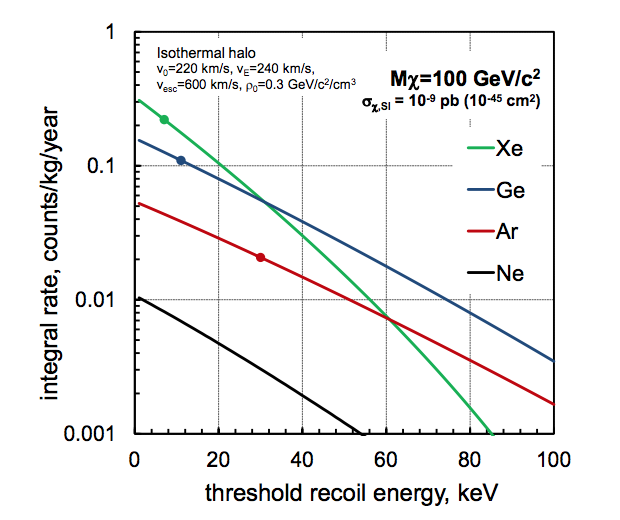
\includegraphics[width=0.65\textwidth]{figures/lxetpcs/wimp_rates.png}
\caption{Plot showing spin-independent WIMP rates in common detector target materials, dots indicate typical thresholds for the targets. Xenon gains in favored SUSY parameter space ($M_{\chi} \gtrsim$ 100~GeV) due to a kinematic enhancement ($M_{\chi} \sim M_{Xe}$ ) and a cross-section enhancement ($\sigma_{SI} \propto A^{2}$). Figure from \cite{Chepel2013}}
\label{fig:wimp_rates}
\end{center}
\end{figure}

\begin{figure}[htbp]
\begin{center}
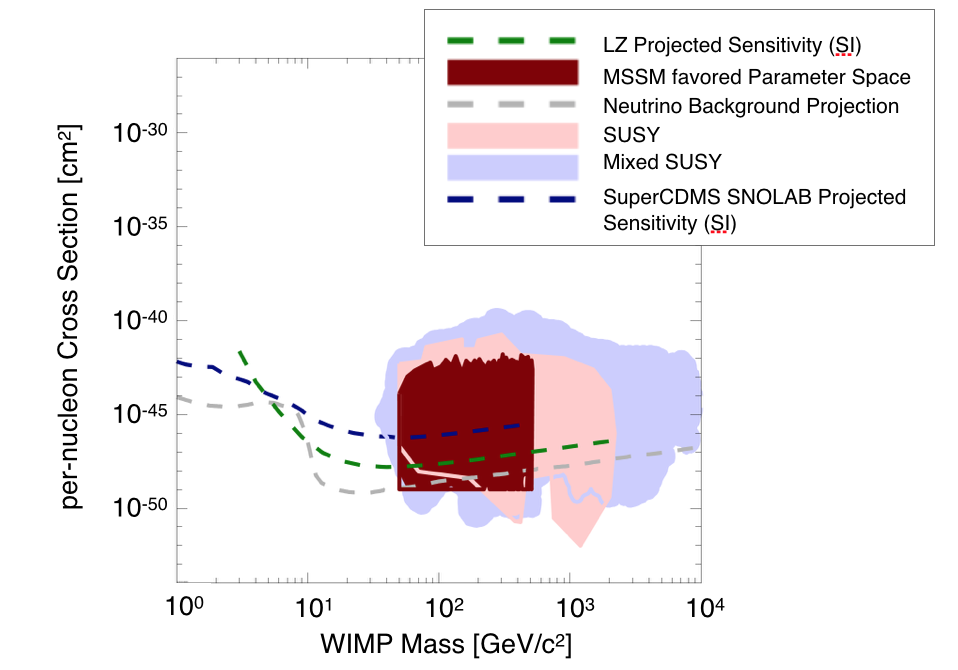
\includegraphics[width=0.65\textwidth]{figures/lxetpcs/WIMPblobs.png}
\caption{Projected limits of next-generation dark matter detectors and areas where SUSY models predict the presence of WIMPs. Although Xe (LZ, green dashed) performs better for WIMP parameter space, Ge and Si (SuperCDMS, blue dashed) can access other light dark matter parameter space below 10~GeV. The plot was generated by http://dmtools.brown.edu/ }
\label{fig:WIMPblobs}
\end{center}
\end{figure}




\subsection{Other Dark Matter Searches with LXe TPCs}
\label{sec:non_wimp_searches_with_lxetpcs}
The available \ac{SUSY} parameter space has dwindled greatly in the last few decades, due in large part to the success of this detector technology. Coupled with no observation of \ac{SUSY} at the \ac{LHC}, experimentalists are beginning to look to other models and parameter spaces for dark matter. New technologies are being developed and refined for new dark matter candidates, but already existing, well-understood detector technologies such as dual-phase \ac{TPC}s can also be employed in the search for non-\ac{WIMP} dark matter. 

In their first \ac{WIMP} search results, the Xenon10 collaborationIn imposed an analysis threshold of $4.5~keV_{nr}$ \cite{Xenon10WIMP}. The first \ac{LUX} results set an analysis threshold of $4.3~keV_{nr}$ (with 2 < S1 (phd) < 30 and S2 (phd) > 200; S2 (electrons) $\gtrsim$ 8) \cite{LUXFirstResults}. The first Xenon100 results set an analysis threshold of $8.7~keV_{nr}$ (4 < S1(phe) < 20 and S2 (phe) > 300; S2(electrons) $\gtrsim$ 10) \cite{Xenon100FirstResults}. Such thresholds are common practice, and are set by the light-collection efficiency of the detector; the detection threshold is much lower. Dual-phase \ac{TPC}s are sensitive to events which produce a single electron, due to the internal amplification of the S2 signal; the reason for setting analysis thresholds is to ensure the presence of an S1 in the event. Without both and S1 and S2 in the event, the full (x,y,z) position cannot be re-constructed, and so a fiducial cut cannot be applied. Sorensen showed that the Xenon10 S2 pulse width carries a mild z-dependence \cite{Sorensen2010}, and so larger detectors with a long drift time may gain reliable z-position reconstruction via S2 pulse width \cite{SorensenS2Width}. Improvements in analysis techniques such as this allow dual-phase xenon \ac{TPC}s to reach lower \ac{WIMP} masses, and even other dark matter models. 

In 2011 the Xenon10 collaboration presented a search for low-mass (\~5 - 20 GeV) dark matter \cite{Angle2011}. The detector conditions were distinct from the Xenon10 \ac{WIMP} search in \cite{Xenon10WIMP}: the secondary scintillation gain was about 12\% higher, and the S2-sensitive trigger threshold was set at the level of a single electron. With this, the collaboration carried out a standard \ac{WIMP} analysis (i.e one based on the procedure presented in \ref{sec:wimp_rates}), with a lowered S2 analysis threshold of 4 electrons ($1.4~keV_{nr}$). Why they did not proceed down to the detection threshold of 1 electron is very interesting; and is discussed further in Chapter~\ref{ch:etrains}. Since Xenon10 is a small detector, they were not able to take advantage of S2-width z-correlations, but they employed a radial fiducial cut and other analysis techniques to produce the result in Figure~\ref{fig:xenon10lowmass}, which also shows the Xenon10 standard \ac{WIMP} analysis for comparison.

\begin{figure}[htbp]
\begin{center}
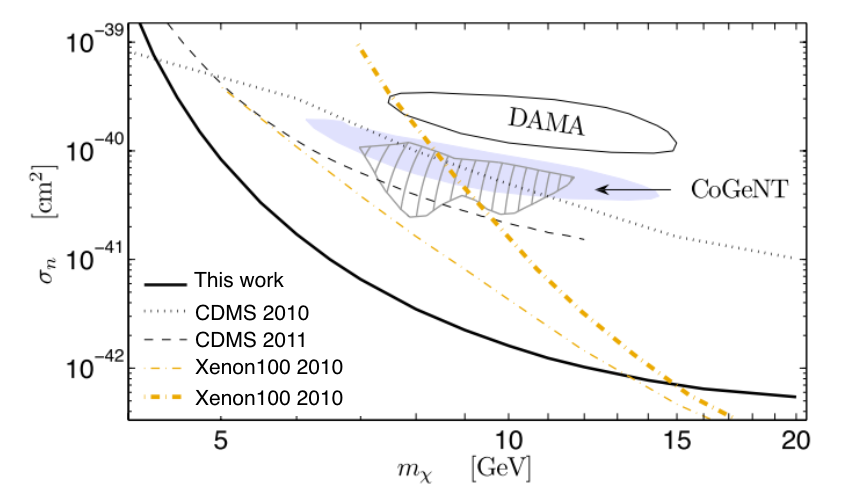
\includegraphics[width=0.65\textwidth]{figures/lxetpcs/xenon10lowmass.png}
\caption{Xenon 10 low-mass WIMP limit extended the range of the standard WIMP result. }
\label{fig:xenon10lowmass}
\end{center}
\end{figure}


A few years later, Essig et al. used the information reported in \cite{Angle2011} and other Xenon10 publications to produce the first direct detection limits of sub-Gev dark matter \cite{Essig2012}. The detection threshold for \ac{WIMP}s in \ac{LXe} decreases sharply for $M_{WIMP} \lesssim 10~GeV$; however, this detection threshold is based on the assumption that the dark matter is interacting only with the xenon nucleus. If sub-GeV dark matter scatters with atomic \textit{electrons}, as opposed to nuclei, then it can produce observable signals of a few electrons. In \ac{LXe} \ac{TPC}s the S1 signal is lost due to light collection, and the few electron signals are observable as S2s. The approach in the paper is to follow approximately the same procedure as in Section~ \ref{sec:wimp_rates}, with a few but significant substitutions. The $E_{R}$ in Equation~\ref{eq:recoil} must now account for the binding energy of the electron, and take a different form to refer to the recoil of the electron and not the nucleus. The cross section of interest is now $\sigma_{e}$, the sum over all of the differential ionization cross sections for electrons in the (n, l) shell. For a dark photon with mass $O$(MeV-GeV) coupled to the visible sector via kinetic mixing (a very generic class of standard model extensions discussed in $Chapter~\ref{sec:dark_sector}$, Essig et al. set the exclusion limit in the $m_{DM}-\sigma_{e}$ plane in Figure~\ref{fig:subGeV} (left). If there is some momentum-transfer enhancement due to e.g. scattering through an electric-dipole moment, $\sigma_{e} \longrightarrow \sigma_{e}F_{DM}(q) \equiv \bar{\sigma_{e}}$. Essig set exclusion limits for such dark matter candidates in Figure~\ref{fig:subGeV} (right).


\begin{figure}[htbp]
\begin{center}
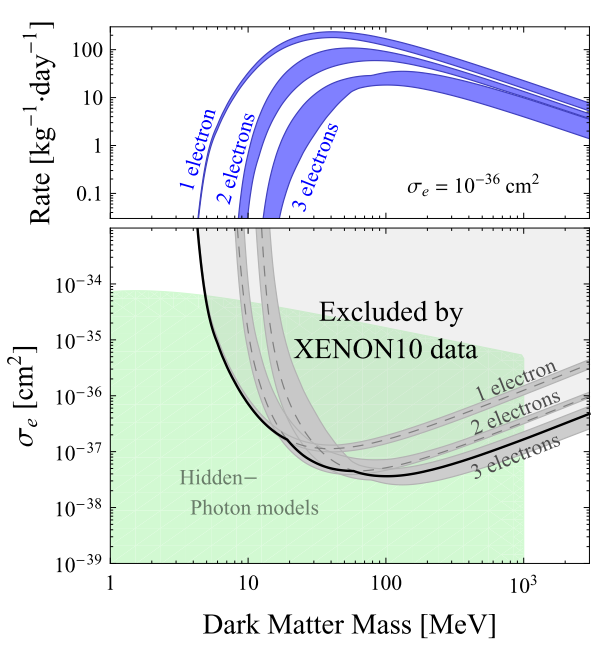
\includegraphics[width=\halffig]{figures/lxetpcs/subGeV.png}
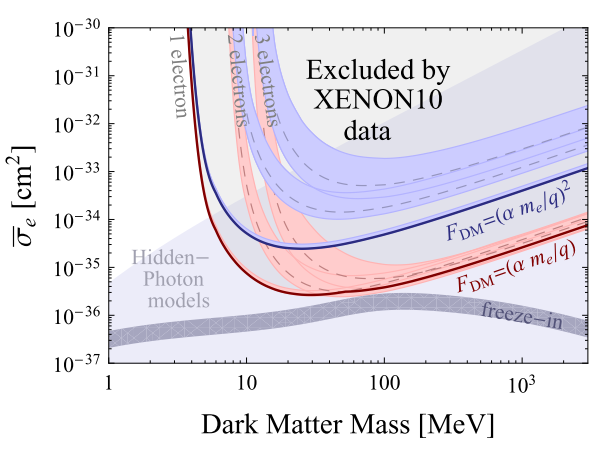
\includegraphics[width=\halffig]{figures/lxetpcs/subGeV2.png}
\caption{(left) Top: Expected 1,2,3-electron signal rates for Sub-GeV DM with $\sigma_{e} = 10^{-36}~cm^{2}$ and Bottom: exclusion limit set with Xenon10 few-electron signals. (right) Exclusion limits for dark matter scattering through an electric-dipole moment (red) and through a very light (<< keV) mediator (blue) }
\label{fig:subGeV}
\end{center}
\end{figure}


In addition to the dark sector, dual-phase \ac{TPC}s can search for other dark matter signals with scattering on electrons. Annual modulation searches (in \ac{ER} or \ac{NR}) can provide clues to dark matter. Such searches take advantage of the fact that $v_{E}$ varies with the rotation of the earth around the sun, reaching a maximum in June and minimum in December. The modulation in $v_{E}$ leads to a modulation in the recoil rate observed in the detector. Searches for dark matter-induced rate modulations can offer a generic approach to identify dark matter interactions, complementary to the model-driven dark matter searches. The \ac{LUX} experiment did such a search, looking at \ac{ER} modulations in an energy rage of interest (2-6~$keV_{ee}$). This energy range was chosen to overlap with the DAMA/LIBRA Collaboration's long-standing and controversial claim of dark matter modulation on a target of NaI(Tl), which appears strongest around a recoil energy of 3~$keV_{ee}$. \ac{LUX} found no significant indication of rate modulation \cite{LUXModulation}. If future large dual-phase \ac{TPC}s like XenonNT and LZ observe a \ac{NR} \ac{WIMP} signal, the additional positive identification of a modulation signal of the \ac{NR} signal would be a smoking-gun for \ac{WIMP} discovery. 

Another dark matter candidate that could produce an electron recoil signal in xenon is the axion (or more generally, axion-like-particles). For searches such as these, a signal model is produced from the spectrum of axions from different sources, such as galactic axions or solar axions. The resulting signal model is an \ac{ER} spectrum accounts for finite detector energy resolution and threshold. The signal model spectrum is compared to the observed \ac{ER} spectrum in the appropriate energy ranges, resulting in a confidence statement mass of the axion $m_{A}$ and the axio-electric coupling $g_{Ae}$. The results of searches for solar axion and galactic axion signals are shown in Figure~\ref{fig:axions}.

\begin{figure}[htbp]
\begin{center}
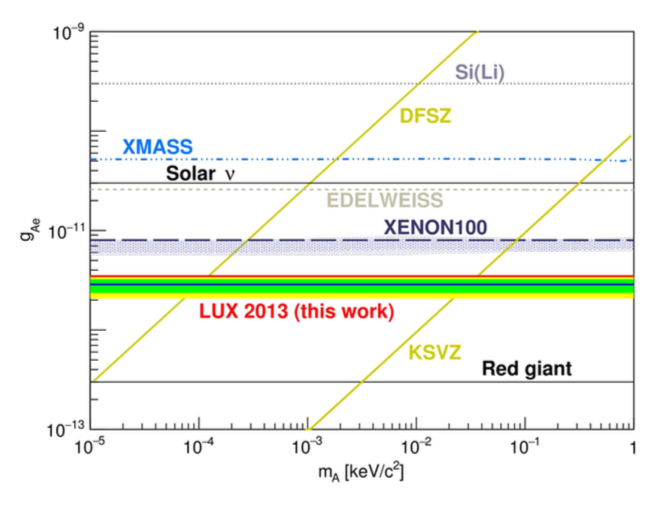
\includegraphics[width=\halffig]{figures/lxetpcs/axions1.png}
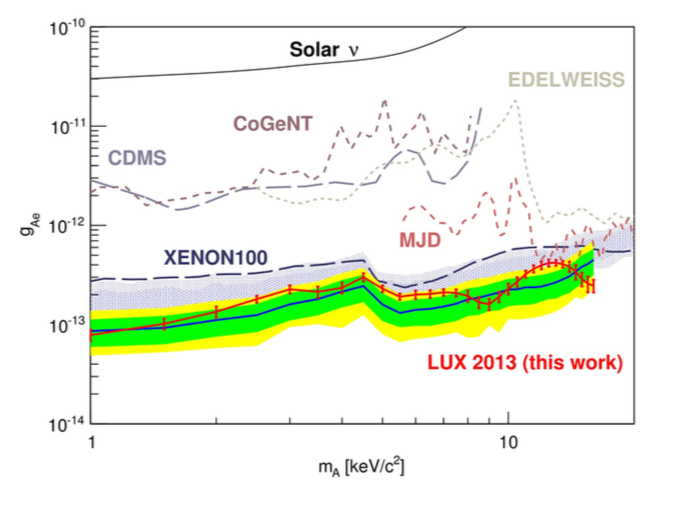
\includegraphics[width=\halffig]{figures/lxetpcs/axions2.png}
\caption{(left) Recent limits on solar axion coupling and mass (right) recent limits on galactic axion coupling and mass. Figure taken from \cite{LUXAxions}. }
\label{fig:axions}
\end{center}
\end{figure}

Finally, a model-independent search for \ac{LIP}s is possible in dual-phase xenon \ac{TPC}. As discussed in Chapter~\ref{sec:dark_sector}, \ac{LIP}s appear in dark sector models with a masses dark photon, where another dark sector particle $\chi$ couples to the standard model electron via kinetic mixing of the dark photon and standard model photon. \ac{LIP}s deposit energies that can be described with particles of effective fractional charge. Chapter~\ref{ch:lips} describes the signal model and analysis method to search for \ac{LIP}s in \ac{LUX}. 





%*****************************************
%*****************************************
%*****************************************
%*****************************************
%*****************************************



\cleardoublepage % Empty page before the start of the next part

%----------------------------------------------------------------------------------------

\ctparttext{This section describes research done with the \acs{LUX} Detector. The \acs{LUX} program is discussed in detail, including key detector components and calibrations. This is followed by a search for cosmogenic \acs{LIP}s. } % Text on the Part 2 page describing the content in Part 2

\part{Big Science}
\label{part:lux}

%************************************************
\chapter{The LUX Detector}

\label{ch:LUX} % $\mathbb{ZNR}$
%************************************************

%\begin{flushright}{\slshape    
%   I'm the hottest in the street \\
%   Know you prolly heard of me } \\ \medskip
%    --- {Cardi B, \textit{Bodak Yellow}, 2017}
%\end{flushright}



\section{LUX Overview}
The \ac{LUX} detector was an ultra-low background dual-phase liquid xenon \ac{TPC} that set world-leading limits on \ac{WIMP} interactions.
 
\ac{LUX} began underground commissioning in July 2012, moving to the 4850 level (4300~m.w.e) of \ac{SURF} in Lead, South Dakota.  The \ac{LUX} Collaboration's first \ac{WIMP} search exposure was for a period of 85.3 live-days, acquired between April 2013 and August 2013. This period of time is referred to as Run03, and the \ac{WIMP} result is referred to as WS2013. The detector then underwent a grid conditioning campaign to improve voltage capabilities, followed by a series of extensive calibrations to characterize the new operating conditions. The detector then ran for a period of 332 live-days from September 2014 to May 2016 (Run04, WS2014-2016), ending with decommissioning in September 2016. Run03 and Run04 had distinct operating conditions and calibrations. The \ac{LIP} search in Chapter~\ref{ch:lips} was carried out using Run03 data, and the calibrations in the latter half of this chapter describe the detector conditions as they were in Run03. 

\section{Internal Components}
The active volume of \ac{LUX} was composed of 300~kg of liquid xenon, instrumented with two arrays of Hamamatsu R8778 \ac{VUV}-sensitive \ac{PMT}s viewing the liquid region from the top and bottom. Both arrays were composed of 61 \ac{PMT}s that detected S1 and S2 photons from particle interactions in the active liquid volume, and were held in place by copper mounting blocks. The \ac{PMT}s were tightly packed in a hexagonal formation to maximize light collection. The xenon-facing surfaces the of copper \ac{PMT} mounting blocks were covered with \ac{PTFE} tri-foils to reflect the 178~nm light, since copper is a poor reflector of \ac{VUV} light. 

The active region was defined by a series of strung wire or mesh grids: the cathode grid was at the bottom of the detector, and the gate grid was 48.3~cm above the cathode when cold. These two grids formed the drift field, which was \~180~kV/cm during Run03. The region is known as the drift region, it is where particle interactions The anode mesh plane was 1~cm above the gate grid, and the xenon liquid level was held constant between these two electrodes by a spillover weir. The anode and gate form the extraction region of the experiment, where electrons are extracted across the liquid-gas boundary and undergo proportional scintillation to form S2. There are two additional grids, the top and bottom grids, which are placed 2~cm from the top and bottom \ac{PMT} arrays to insulate the \ac{PMT}s from the high fields produced by the other grids. The top and bottom grids were held at approximately the same voltage applied to the \ac{PMT}s. All electrodes were 88\%-99\% optically transparent at normal incidence, and made of stainless steel 316. The major components of \ac{LUX} are shown in Figure~\ref{fig:lux1}

\begin{figure}[htbp]
\begin{center}
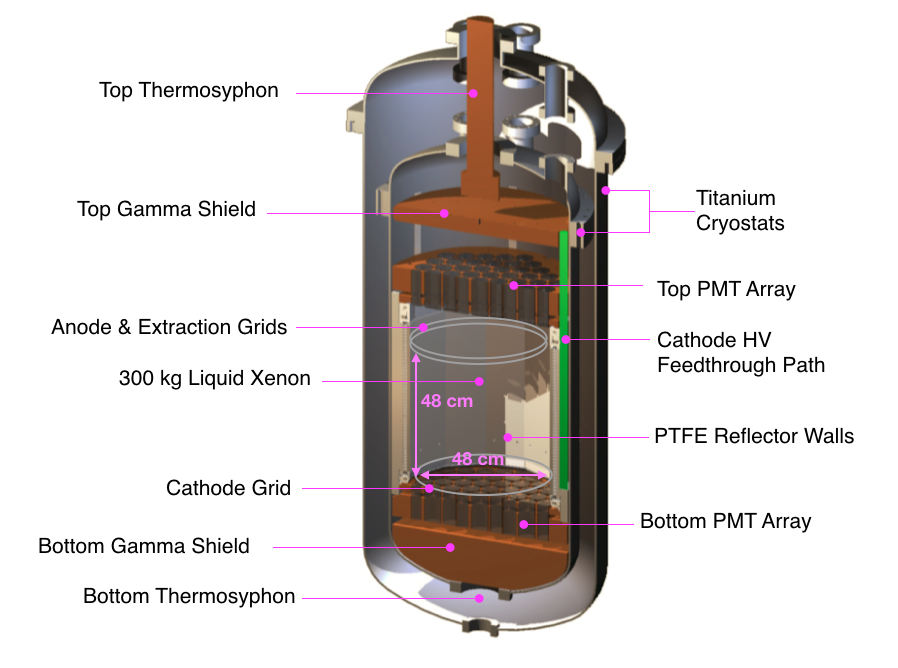
\includegraphics[width=\textwidth]{figures/lux/lux_inner1.png}
\caption{Major components and dimensions of the LUX detector.}
\label{fig:lux1}
\end{center}
\end{figure}


The insides of the detector walls were lined with 12 \ac{PTFE} panels, which made the exact detector geometry a dodecagonal prism with flat faces, instead of a cylinder one rounded face. Immediately behind the \ac{PTFE} were 48 copper field-shaping ``rings'' (dodecagons). The rings were vertically separated by 1~cm, and the gate-to-cathode voltage was graded evenly over the rings by a resistor chain connecting the rings. 

Below and above the \ac{PMT} mounting blocks were two large solid copper domes which act as gamma shields and also function as thermal mass that aid in keeping the detector temperature stable. The bottom dome also acts as a heat exchanger to quickly re-thermalize incoming xenon gas (from the circulation system) as it enters the liquid region, and minimizes the volume filled with non-active liquid xenon. See Figure~\ref{fig:lux2} for details of the field-shaping rings and copper shields.

\begin{figure}[htbp]
\begin{center}
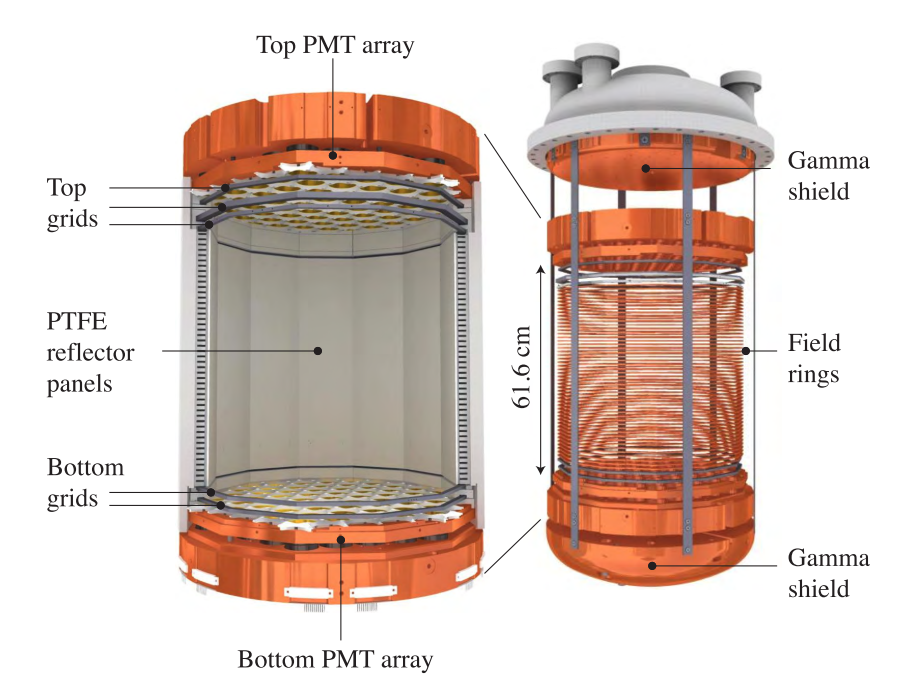
\includegraphics[width=\textwidth]{figures/lux/lux_inner2.png}
\caption{Field-shaping rings detail}
\label{fig:lux2}
\end{center}
\end{figure}


More details about the internal components can be found in C. Faham's PhD thesis \cite{Faham2014a}.

\section{External Components}

The \ac{LUX} cryogenic system was based on thermosyphons, which deliver ``cooling power'' to solid copper cold heads, which are in thermal contact with the liquid xenon space. A simplified diagram is shown in Figure~\ref{fig:luxcryo}. A thermosyphon is a closed-loop cooling device containing a thermal messenger gas; N$_{2}$ is a common choice and was the choice for the \ac{LUX} thermosyphons. The top of the thermosyphon is immersed in a bath of liquid nitrogen, and the bottom is in thermal contact with the liquid xenon space. The internal messenger gas condenses at the top and drips down to the cold head, where it absorbs heat from the xenon space, evaporates, and returns to the top of the thermosyphon to condense and repeat the cycle. In this manner, heat from the liquid xenon space is transferred to the external nitrogen bath, which boils off and must be periodically replenished. The pressure of the internal nitrogen messenger gas can be adjusted, providing more or less cooling power as desired. The \ac{LUX} thermosyphons were also instrumented with resistive heaters, for further fine control. Four thermosyphons were used to operate the \ac{LUX} detector stably at \~175~K with a xenon vapor pressure of \~2~bar. 

\begin{figure}[htbp]
\begin{center}
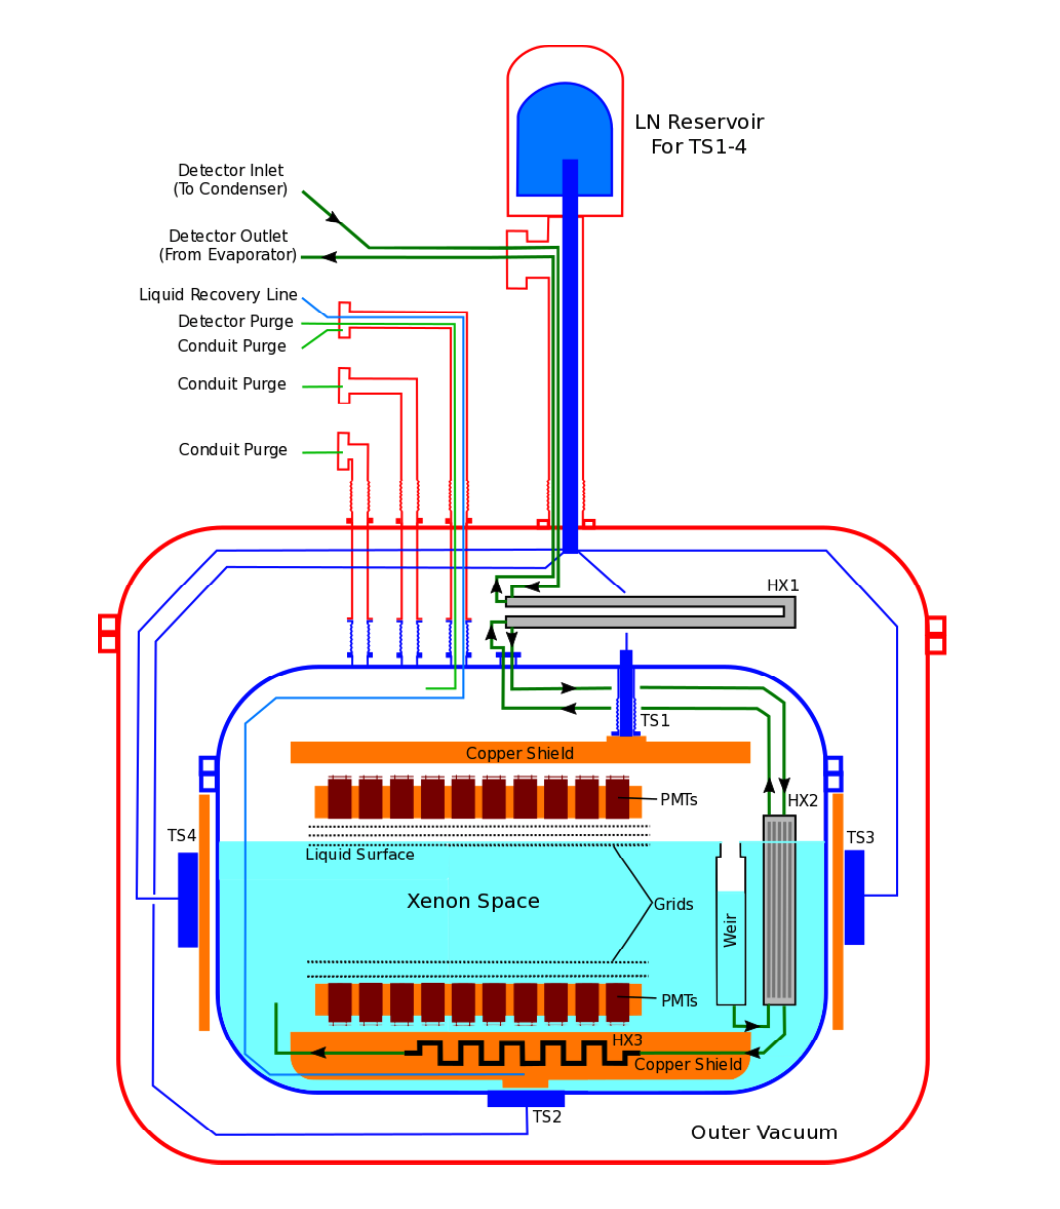
\includegraphics[width=\textwidth]{figures/lux/lux_cryostats.png}
\caption{A simplified diagram of the LUX cryogenic system. \cite{Larsen2016}}
\label{fig:luxcryo}
\end{center}
\end{figure}

The spillover liquid xenon from the liquid-level-setting weir mentioned above was directed into a circulation system through a series of heat exchangers that helped cool clean, incoming xenon gas. The xenon circulation was driven by one twin-head KNF double-diaphragm pump, which pushed liquid xenon from the spillover weir through a SAES MonoTorr heated zirconium getter to remove non-noble impurities before returning the clean xenon gas into the detector. A sampling system was able to pull xenon gas samples from different parts of the circulation system and measure impurity content, as well as test for the presence of $^{85}$Kr \cite{Dobi2011}, a troublesome beta emitter which must be removed from the xenon prior to carrying out a successful \ac{WIMP} search.

The circulation pump was installed in parallel with a backup pump, which could be switched on immediately in case of a pump outage. Flow was regulated to the system by two high-flow \ac{MFC}s. Additional low-flow \ac{MFC}s controlled purge flow through the cabling conduits in Figure~\ref{fig:luxcryo} to ensure gas flow was away from the detector and prevent any contaminants from diffusing into the active xenon space.

Internal calibration sources were plumbed in to alternate flow paths of the circulation system. Xenon gas could be directed through a substrate source, such as the $^{83m}$Kr source described below, to pull $^{83m}$Kr into the detector volume. A bottle containing a source such as the CH$_{3}$T source described below could be used to deposit the gaseous source in an evacuated section of pipe. Xenon could then be directed through the section of pipe containing the source, sweeping it into the detector volume. 

Lastly, \ac{LUX} was placed in a 7.6~m diameter, 6.1~m high water tank (Figure~\ref{fig:luxwatertank}). The shielding provided by the water tank attenuated the $\gamma$ background from the cavern walls and thermalized neutrons from cavern background radioactivity and muon spallation. The water tank provided superior shielding from cavern radioactivity such that the detector backgrounds were dominated by the radioactivity of internal detector components, which in turn were controlled through a strict campaign of cleanliness and choice of detector materials \cite{LUXDetectorPaper}, \cite{LUXRun03Backgrounds}. Vertical tubes visible in Figure~\ref{fig:luxwatertank} were used to deploy external calibration sources at different heights, such as $^{137}$Cs, which were directed into the detector via a collimating source assembly.


\begin{figure}[htbp]
\begin{center}
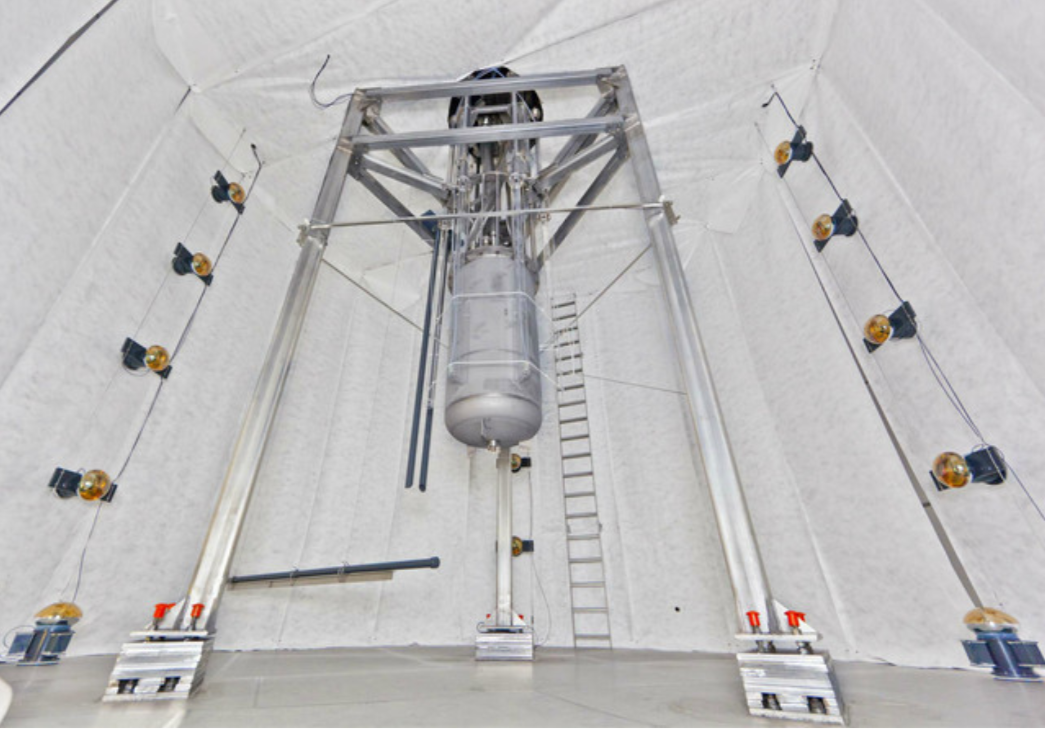
\includegraphics[width=\textwidth]{figures/lux/lux_watertank.png}
\caption{A photo of the LUX detector installed inside the water tank.}
\label{fig:luxwatertank}
\end{center}
\end{figure}

The \ac{LUX} detector water tank and material screening achieved a very low background in the \ac{WIMP} search energy range shown in Figure~\ref{fig:luxrun03bkg}

\begin{figure}[htbp]
\begin{center}
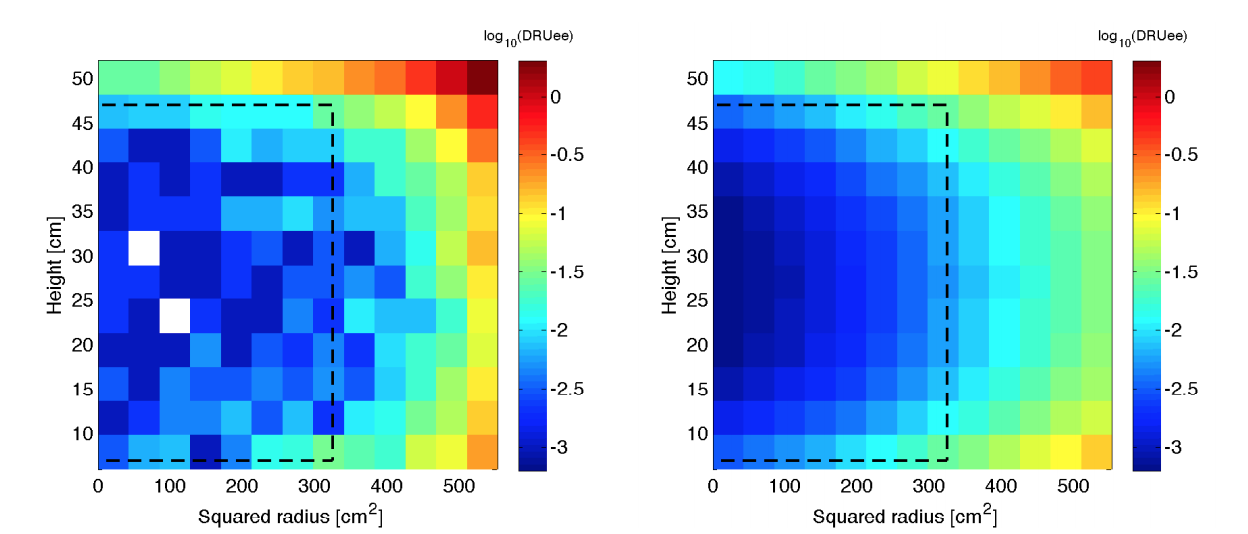
\includegraphics[width=\textwidth]{figures/lux/lux_run03bkg.png}
\caption{Backgrounds distributions in squared radius and height for expected (right) and measured (left) backgrounds in the energy range 0.9-5.3~keV$_{ee}$ (2-30 phe S1) for the 85.3 live-day Run03 \ac{WIMP} exposure. Black lines show the 118~kg fiducial mass. Units are log$_{10}$DRU$_{ee}$, electron equivalent differential rate units, i.e. keV$_{ee}^{-1}$kg$^{-1}$day$^{-1}$.  Figure from \cite{LUXRun03Backgrounds}. }
\label{fig:luxrun03bkg}
\end{center}
\end{figure}


\section{Trigger and Data Acquisition}
Cabling for PMTs and other monitoring instrumentation were routed from the inner detector volume to the outside via conduits illustrated in in Figure~\ref{fig:luxcryo}. A flow char illustrating the signal path is shown in Figure~\ref{fig:luxdaq}. 

\begin{figure}[htbp]
\begin{center}
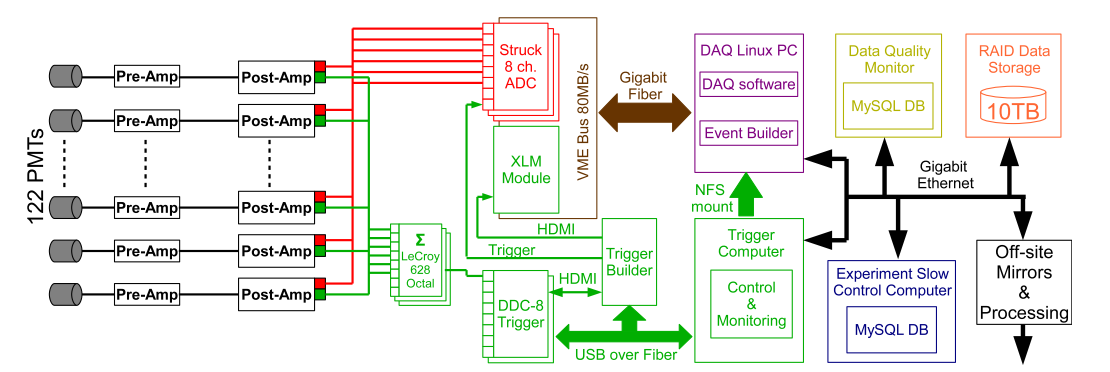
\includegraphics[width=\textwidth]{figures/lux/lux_daq.png}
\caption{Overview of the LUX trigger system. Figure from \cite{LUXTrigger}. }
\label{fig:luxdaq}
\end{center}
\end{figure}


The \ac{PMT} signals were shaped and amplified by two sets of amplifiers. These analog voltage waveforms were then digitized by Struck \ac{ADC}s, with 14 bit, 100~MHz sampling (1 sample every 10~ns). A copy of the analog \ac{PMT} voltage waveforms passed through the \ac{LUX} \ac{FPGA} trigger system, which signaled the data acquisition computer to save the waveforms when they passed above a certain threshold, and stop when they fell below the threshold. Each of the 122 \ac{PMT}s was dedicated its own channel in the recorded data, so recording only the channels that passed threshold allowed for a great amount of data reduction. This technique is called \ac{POD}. A \ac{POD} threshold of 1.5~mV was used for \ac{LUX}, which resulted in a single photoelectron efficiency of > 95\% \cite{LUX:Run03Comprehensive}. A figure showing the \ac{POD} threshold and example waveform are shown in Figure~\ref{fig:waveforms}. 


\begin{figure}[htbp]
\begin{center}
%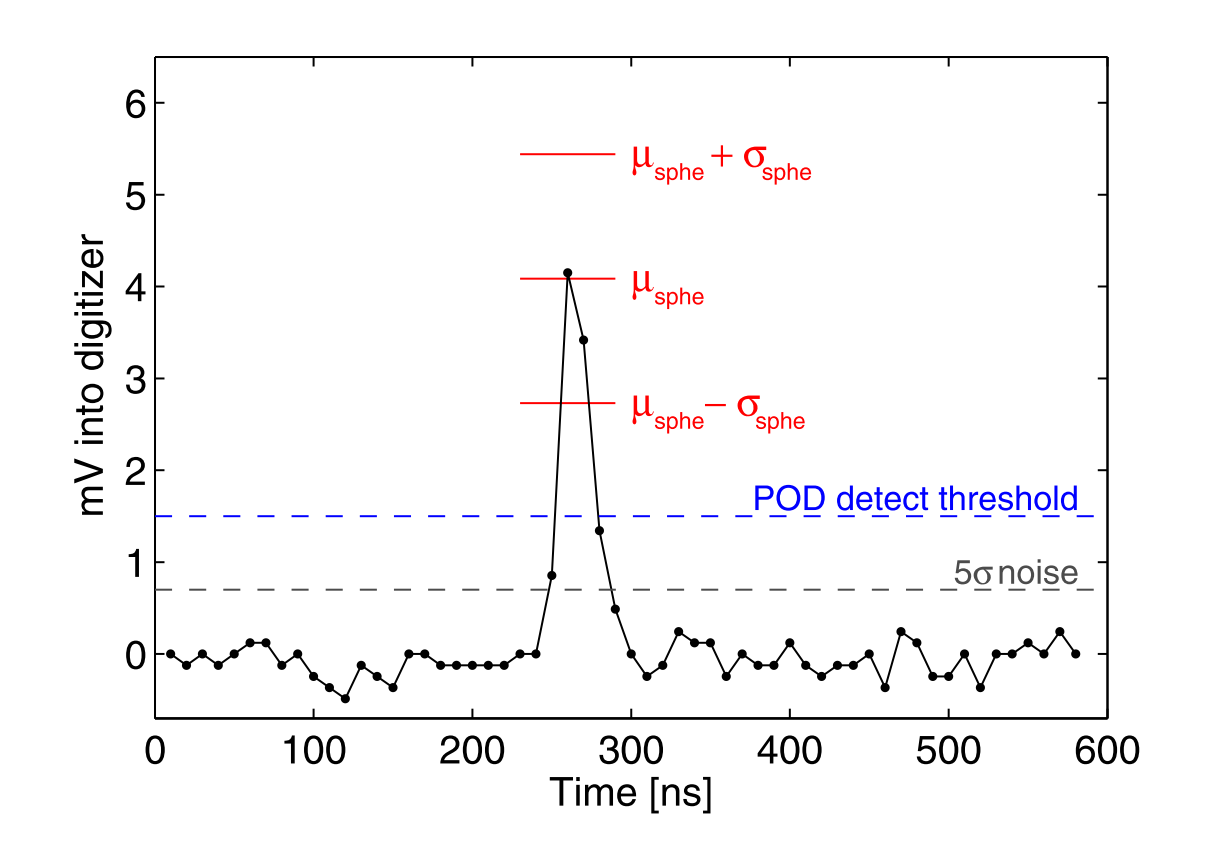
\includegraphics[width=0.29\textwidth]{figures/lux/pod_detect.png}
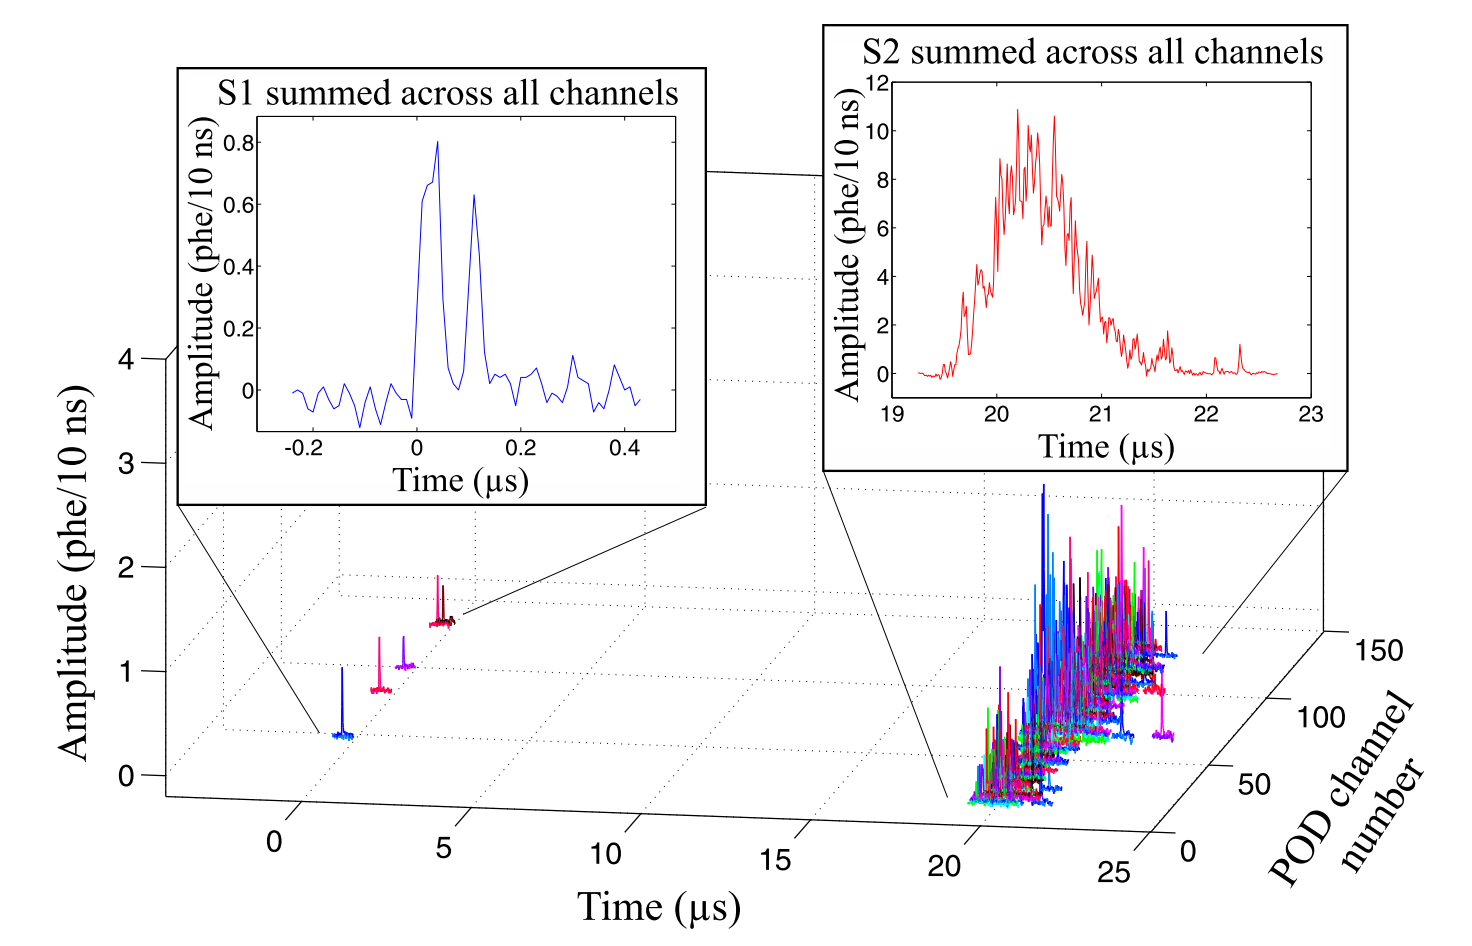
\includegraphics[width=\textwidth]{figures/lux/sample_waveform.png}
\caption{An example recorded event. Channels that do not pass the POD threshold are not recorded. The waveforms are summed over all channels to produce the S1 and S2 \cite{LUXTrigger}. }
\label{fig:waveforms}
\end{center}
\end{figure}

The channel-wise \ac{POD} data is written continuously to disk as the \ac{ADC} memory buffer fills; this is the rawest and least filtered form the \ac{LUX} data that is saved in binary format with the \textbf{.dat} extension. The Event Builder takes the takes the raw data and extracts portions located in a pre-trigger and post-trigger window. A additional hold-off time is applied after the post-trigger window to assure \ac{POD}s are not duplicated the subsequent event. The pre- and post- trigger windows for Run03 were set to be 500~$\mu$s, chosen to ensure both S1 and S2 pulses were contained in the same event. The maximum electron drift time in Run03 was 322~$\mu$s, so a pre- and post- trigger time of 500~$\mu$s ensured no S2 would appear without its partner S1. Both types can pass the \ac{POD} threshold and signal the \ac{DAQ} computer to save the waveforms, but some small S1s are may not cross the threshold and must are ``found'' only at the event-building stage.
The Event Builder then saved the waveform data in binary format with the \textbf{.evt} extension.


\section{Data Processing}
After event-building, the waveform \textbf{.evt}-files were sent off site for additional processing. The \ac{LUX} \ac{DPF} extracts essential information from the waveforms and produces \ac{RQ} files with the \textbf{.rq} extension. The \ac{DPF} is modular, and can be applied repeatedly to the same \textbf{.evt} data with different settings if desired. \ac{RQ} files include event-level information (e.g. trigger timestamp), pulse-level quantities (e.g. pulse type, pulse area), and some channel-level quantities (e.g. pulse area recorded by each \ac{PMT}). The \ac{DPF} classifies pulses as one of five types: S1, S2, \ac{SPHE}, \ac{SE}, and Else (for pulses that do not fit one of the previous four types). The pulse-finding and classification algorithm was designed and optimized for the \ac{WIMP} search, and is crucial in identifying \ac{WIMP} ``golden events'', which are single-scatter interactions with only one S1 and one S2 in the event. Detector backgrounds such as gammas often scatter more than once in the active volume, producing an event with one S1 and multiple S2s. The pulse-finder and classifier also play a large role in \ac{LIP} search, which is discussed more in Chapter~{ch:lips}. An example of pulse identification for a multiscatter event is shown in Figure~\ref{fig:lux_pulses}

\begin{figure}[htbp]
\begin{center}
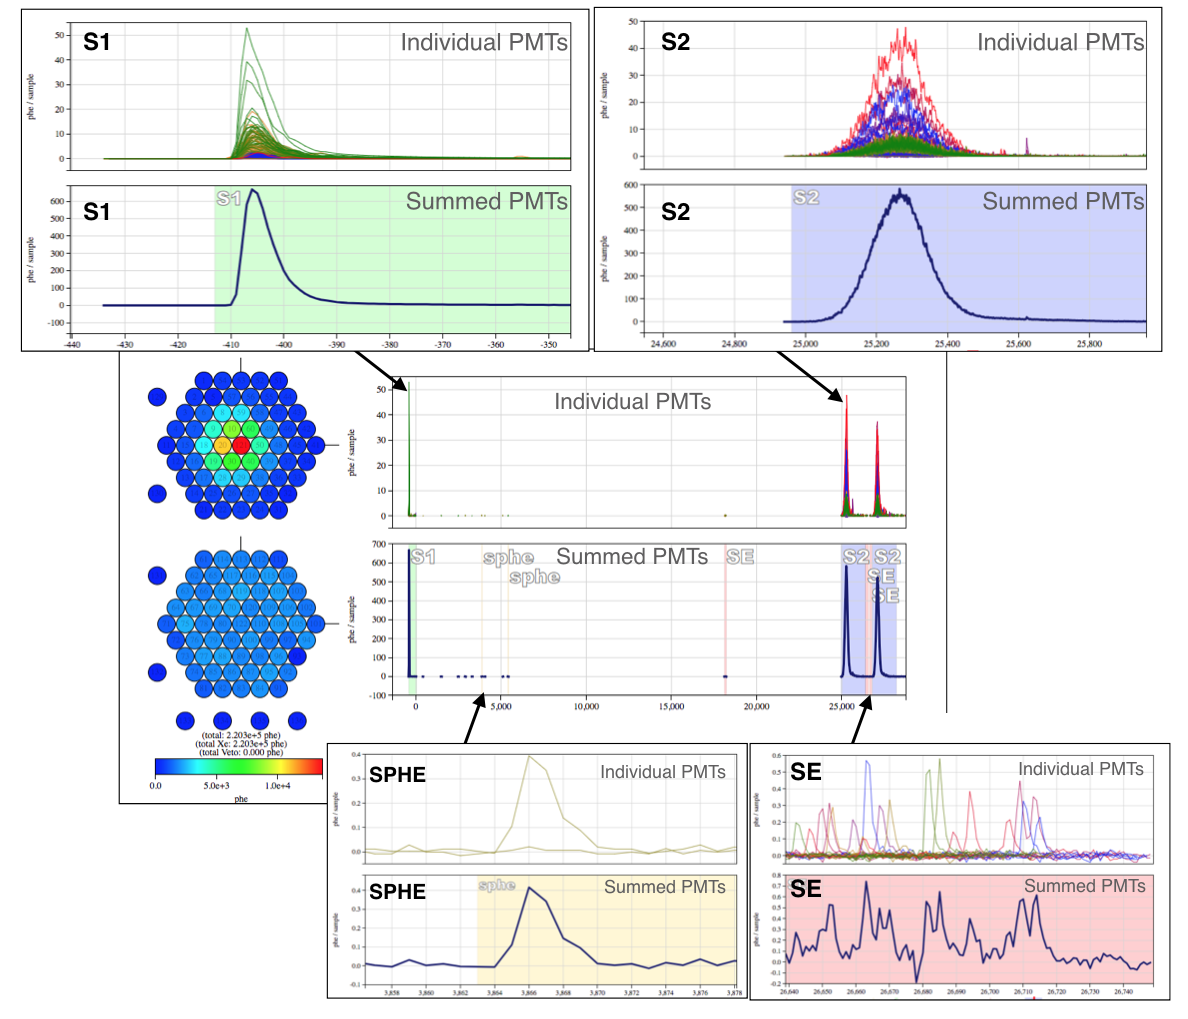
\includegraphics[width=\textwidth]{figures/lux/lux_pulses.png}
\caption{An example of \ac{LUX} pulse classification showing individual pulses. }
\label{fig:lux_pulses}
\end{center}
\end{figure}


Following identification of S1 and S2 pulses, the \ac{DPF} position reconstruction module is run. This module uses the Mercury algorithm, originally developed for the ZEPLIN-III \ac{LXe} \ac{TPC} \cite{Currie2012}, which is based on maximum-likelihood to find the best (x,y) position of the event. Mercury uses \ac{LRF}s, obtained for each \ac{PMT}, to predict the response of the \ac{PMT} to interactions at some arbitrary position of the \ac{PMT}. The \ac{LRF}s were obtained using calibration data, of which $^{83m}$Kr was the most important for position reconstruction. The position reconstruction method and \ac{LRF}s are discussed in more detail in \cite{LUXPositionReconstruction}.


The \ac{DPF} also applies calibration constants to the data. Calibration constants, many of which change over time, are tracked and recorded in the \ac{LUG}, which produces date-specific record files in XML format, which in turn determine the settings for some of the \ac{DPF} modules. For example, the $^{83m}$Kr calibration (see Section~\ref{sec:krypton}) was used to normalize S1 pulse areas. The photon detection efficiency for S1s varies with z-position, with events occuring near the bottom \ac{PMT}s \~50\% more likely to be detected than those near the liquid-gas boundary. The \ac{DPF} applies corrections like this to several RQs, and both the corrected and uncorrected versions are kept. 


\section{Calibrations}
Several novel calibration methods were developed by the \ac{LUX} Collaboration to fully characterize the detector. The superior self-shielding ability of \ac{LXe} detectors also makes them difficult to calibrate. Sources placed external to the detector cannot penetrate the fiducial volume very effectively; since high-statistics are desired for calibration data, relying on external sources becomes untenable. The solution, then, is counterintuitive: purposely introduce radioactive material into painstakingly developed, ultra low-background, fiducial volume of the detector. For such a source to not destroy the ability to carry out a \ac{WIMP} search, it must either (i) be short lived or (ii) be effectively removed by getter on a short timescale. \ac{LUX} demonstrated that $^{83m}$Kr fit the former \cite{LUXKr} requirement and tritiated methane (CH$_{3}$T) fit the latter \cite{LUXTritium}.

\subsection{Energy}
This section covers the energy calibration of \ac{LUX}. Recall from Section~\ref{sec:energy_reconstruction} that the electron-equivalent energy of an event in a dual phase xenon \ac{TPC} is reconstructed as follows:

\begin{equation}
E = W (\frac{S1}{g_{1}} + \frac{S2}{g_{2}})
\end{equation}

Two or more calibration line sources of different energies are required to fit for the detector gains $g_{1}$ and $g_{2}$. The \ac{LUX} experiment used a suite of sources to calibrate the energy response of the detector, shown in \ref{fig:calib_sources}. The $^{83m}$Kr is an injected source distributed in the entire internal volume. The $^{137}Cs$ is an external source lowered at different heights into the source tubes. The xenon lines, $^{131}$Xe, $^{129}$Xe $^{127}$Xe, are of cosmogenic origin and were only present early in Run03.

\begin{figure}[htbp]
\begin{center}
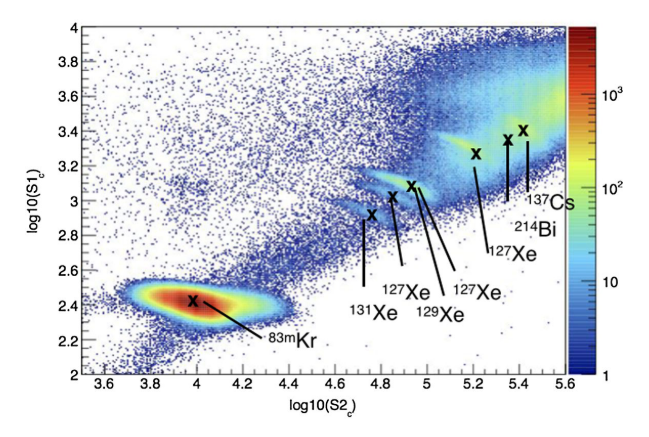
\includegraphics[width=\textwidth]{figures/lux/calibration_sources.png}
\caption{Plot showing calibration sources (Figure from \cite{LUX:Run03Comprehensive}. The axis label subscript $c$ denotes corrected variables with calibration for geometrical effects and electron lifetime (these corrections are discussed in Section~\ref{sec:krypton}.}
\label{fig:calib_sources}
\end{center}
\end{figure}

The average S1 and S2 of each calibration source is normalized to the true energy:

\begin{equation}
(S1, S2) \longrightarrow \Big(\frac{\langle S1 \rangle}{E}, \frac{\langle S2 \rangle}{E}\Big)
\end{equation}

and a line $y = mx + b$ is fit to the transformed variables, where the slope is $m = -g_{1} / g_{2}$ and the y-intercept is $b = g_{1} / W$. Such a plot is called a Doke plot. The sources from figure Figure~\ref{fig:calib_sources} are shown normalized in a Doke plot in Figure~\ref{fig:doke}.

\begin{figure}[htbp]
\begin{center}
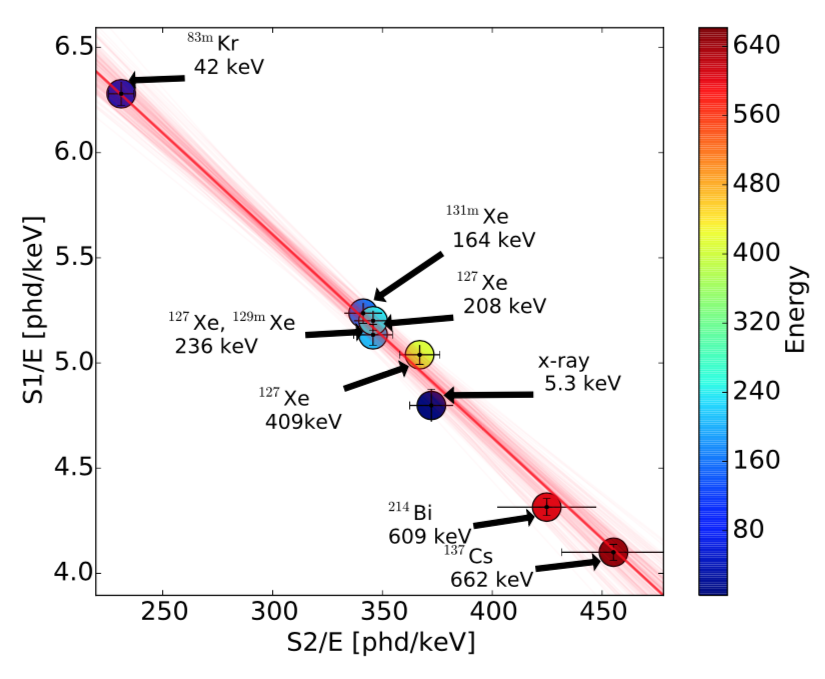
\includegraphics[width=\textwidth]{figures/lux/doke.png}
\caption{ Doke plot used to fit $g_{1}$ and $g_{2}$ for LUX Run03 (Figure from \cite{LUX:Run03Comprehensive}}
\label{fig:doke}
\end{center}
\end{figure}

From the fit in Figure~\ref{fig:doke}, the \ac{LUX} gains for Run03 were measured to be $g_{1} = 0.117 \pm 0.003$~phd/photon and $g_{2} = 12.1 \pm 0.8$~phd/electron. $g_{2}$ depends on a combination of the \ac{EEE} and the number of photons produced by a single extracted electron -- it is useful to know both values. Single electrons are periodically emitted into the gas and undergo proportional scintillation. This phenomenon is well known in liquid xenon detectors and is discussed further in Chapter~\ref{ch:etrains}. A sample of pure single electrons was collected to find the average number of S2 photons produced by one electron, referred to the single electron size. The single electron size in Run03 was a skew-gaussian with mean 24.66 phd and a 1-$\sigma$ width of 5.95 phd. Combing this with $g_{2}$ gives an \ac{EEE} of $49\% \pm 3\%$ \cite{LUX:Run03Comprehensive}.

\subsection{Metastable Krypton-83 ($^{83m}$Kr): A Multifunction Calibration}
\label{sec:krypton}
The $^{83m}$Kr source used by \ac{LUX} was $^{83}$Rb deposited on a charcoal substrate. Gaseous xenon within the circulation system was diverted over the charcoal substrate, where it could sweep $^{83m}$Kr on a flow path through the getter, and then into the detector. 

$^{83m}$Kr decays by two steps releasing a total energy of 41.5~keV. The two branching ratios that dominate are first the internal conversion and subsequent Auger emission of a 32.1~keV $\beta$ followed by another internal conversion and Auger emission of a 9.4~keV $\beta$, with an intervening half-life of 154~ns. The time structure of the decay sometimes yields two S1s, called S1a and S1b. If the second 9.4~keV $\beta$ is prompt (i.e within the timing resolution of the detector), then only one S1 is observed. The S2s are always merged because (1) the low energy of the decays made the energy depositions O(10~$\mu$m) from each other, smaller than the position resolution of the detector O(1~mm) (2) the close timing of the two decays was smaller than the typical electron diffusion distances during drift O(1~mm), merging the two electron bunches together into one S2 \cite{LUXKr}.

$^{83m}$Kr was a workhorse calibration source for \ac{LUX}, with $^{83m}$Kr injections performed weekly at activities ranging from ~10~Bq to hundreds of Bq, depending on the specific calibration goal. $^{83m}$Kr was found to mix uniformly in the detector within \~10~min of the injection, and would decay (half life 1.83~hours) back to an acceptable \ac{WIMP} search background rate within a day, or few days, depending on the injected activity \cite{LUXKr}. The combined energy of the $^{83m}$Kr was well out of the \ac{WIMP} search energy range, so no long-term pollution, though unlikely, was risked. $^{83m}$Kr was used for two main calibrations, described below.

\textbf{Pulse Area Corrections} Detector efficiencies and gains can vary over time and position within the detector. $^{83m}$Kr served as a ``standard candle'', which produced monoenergetic signals with uniform initial light and charge yields distributed uniformly throughout the active volume. The efficiency for detecting the initial light yield as an S1 was dominated by spatially varying geometrical light detection efficiency. The areas of the S1s were binned in 3D, and the averages were found for each bin. A correction map was then constructed as the inverse of the S1 areas, normalized to the S1 amplitude at the center of the detector. The map of relative S1 amplitudes in Figure~\ref{fig:kr_1} (left) shows the strong $z$-dependance for S1 light collection. The corrections for S2 areas were more complex, as detection efficiency for the initial charge yield as an S2 depends on a the presence of electronegative impurities, electron extraction efficiency, production of proportional scintillation photons, and then detection of those photons in PMTs. The $xy$- and $z$- dependence for S2s are corrected in two separate maps. The electronegative impurities caused a strong z-dependence in S2 size -- events originating at the bottom of the detector must drift longer and so were more likely to encounter and lose electrons to impurities. The $z$-dependent S2 area correction map was an exponential function of drift time, normalized to unity at the liquid surface. The $xy$-dependence was from detector conditions such as pressure, liquid level, and electric field deflection from the grid. The $xy$-correction map for S2s was normalized to (0,0) in the x-y plane. Examples of both the $z$ and $xy$ S2 area correction maps can be seen in Figure~\ref{fig:kr_1} (right).

\begin{figure}[htbp]
\begin{center}
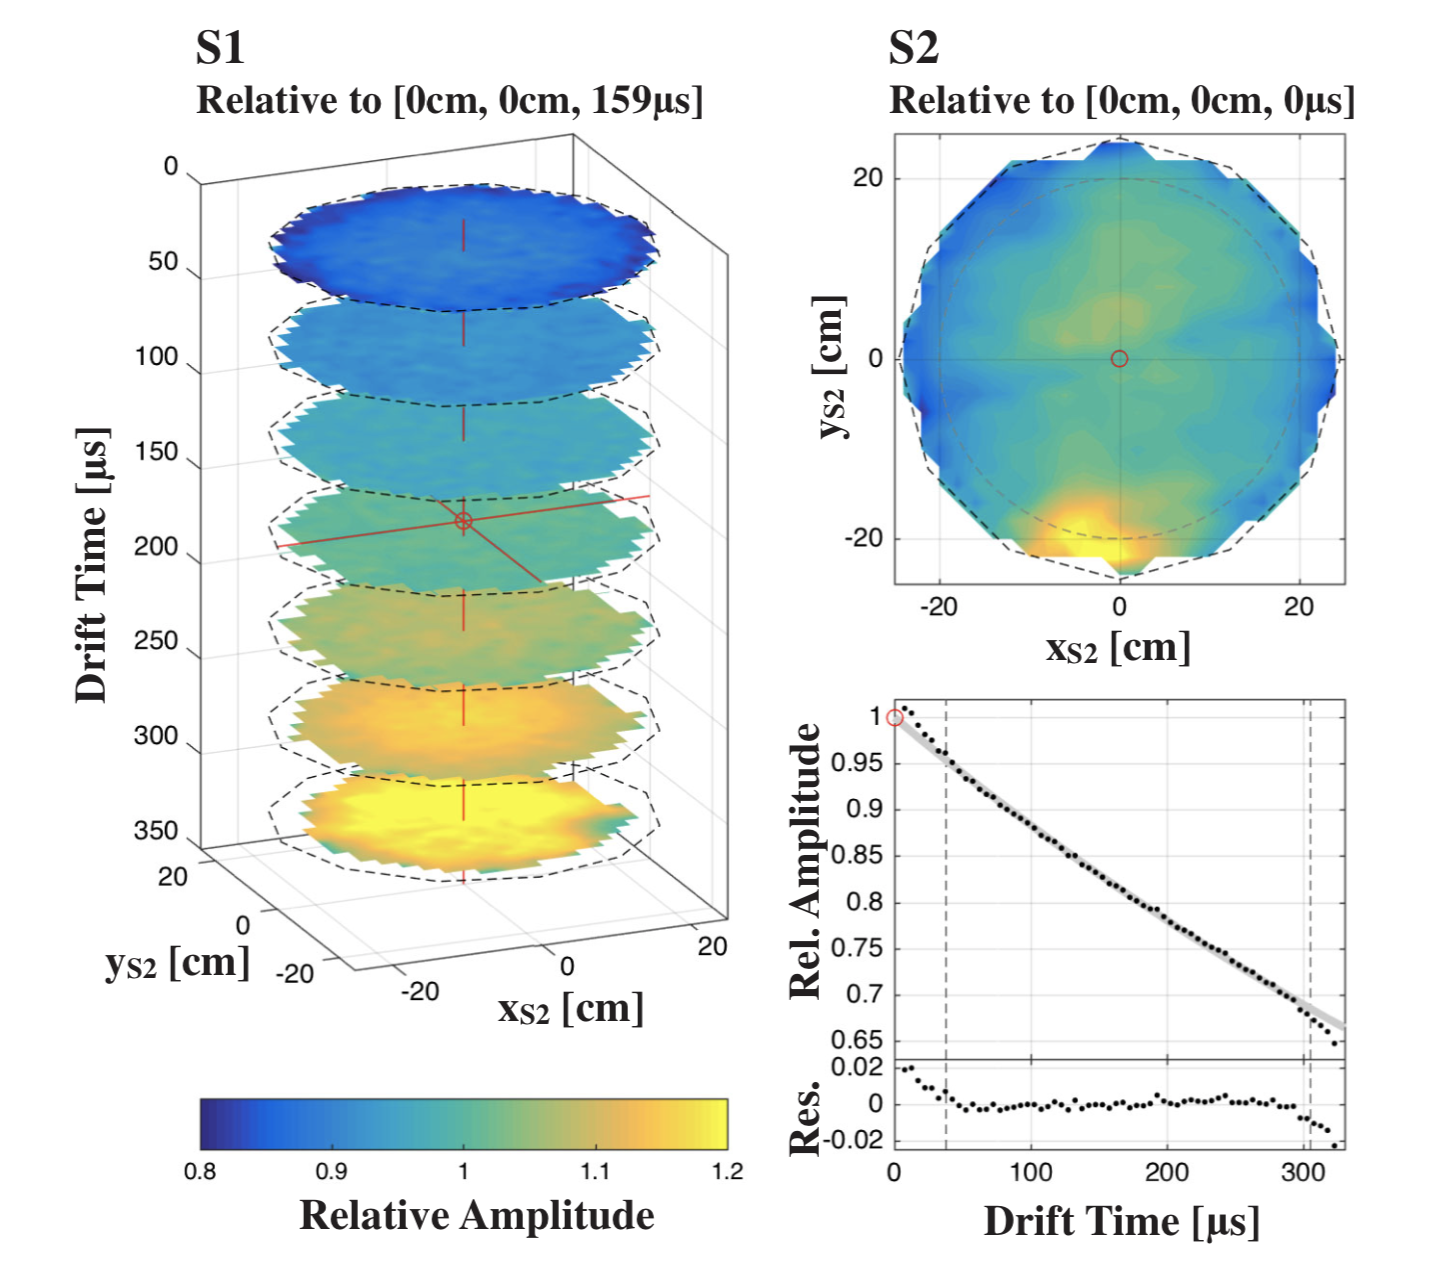
\includegraphics[width=\textwidth]{figures/lux/kr_1.png}
\caption{ Spatial dependence of pulse area corrections for S1 (left) and S2 (right) from an example $^{83m}$Kr calibration. The red circle indicates normalization point. (Figure from \cite{LUXKr}}
\label{fig:kr_1}
\end{center}
\end{figure}

\textbf{Position Corrections} 3D position reconstruction depends on a full understanding of the path electrons take from an interaction site to the position observed after extraction at the surface. The reconstructed position of the proportional scintillation signal in the xy-plane, based on the Mercury algorithm, is referred to ``S2 coordinates", often with subscripts (x$_{S2}$, y$_{S2}$). The real coordinates may be displaced from (x$_{S2}$, y$_{S2}$) due to, for example, a radial field pushing electrons inwards deep in the detector. In fact, there was a small radially inward component to the electric fields in \ac{LUX} Run03 due to the geometry of the field cage and grids (Figure~\ref{fig:kr_pos1}). The spatial distribution of reconstructed $^{83m}$Kr events was used to verify a COMSOL multiphysics electric field model of the detector by drifting electrons in simulation under the electric field model conditions. This field model could then be used to transform events from S2 coordinates to real (x,y) coordinates, however this was not done for Run03. Instead, the $^{83m}$Kr data itself was found to be more precise in for position corrections, since it didn't rely on the accuracy of the field model or electron drift simulation (Figure~\ref{fig:kr_pos2}). The electric field conditions were very different in Run04, and so extensive calibrations and field maps were used to map S2 coordinates to real coordinates \cite{LUXFields}.

\begin{figure}[htbp]
\begin{center}
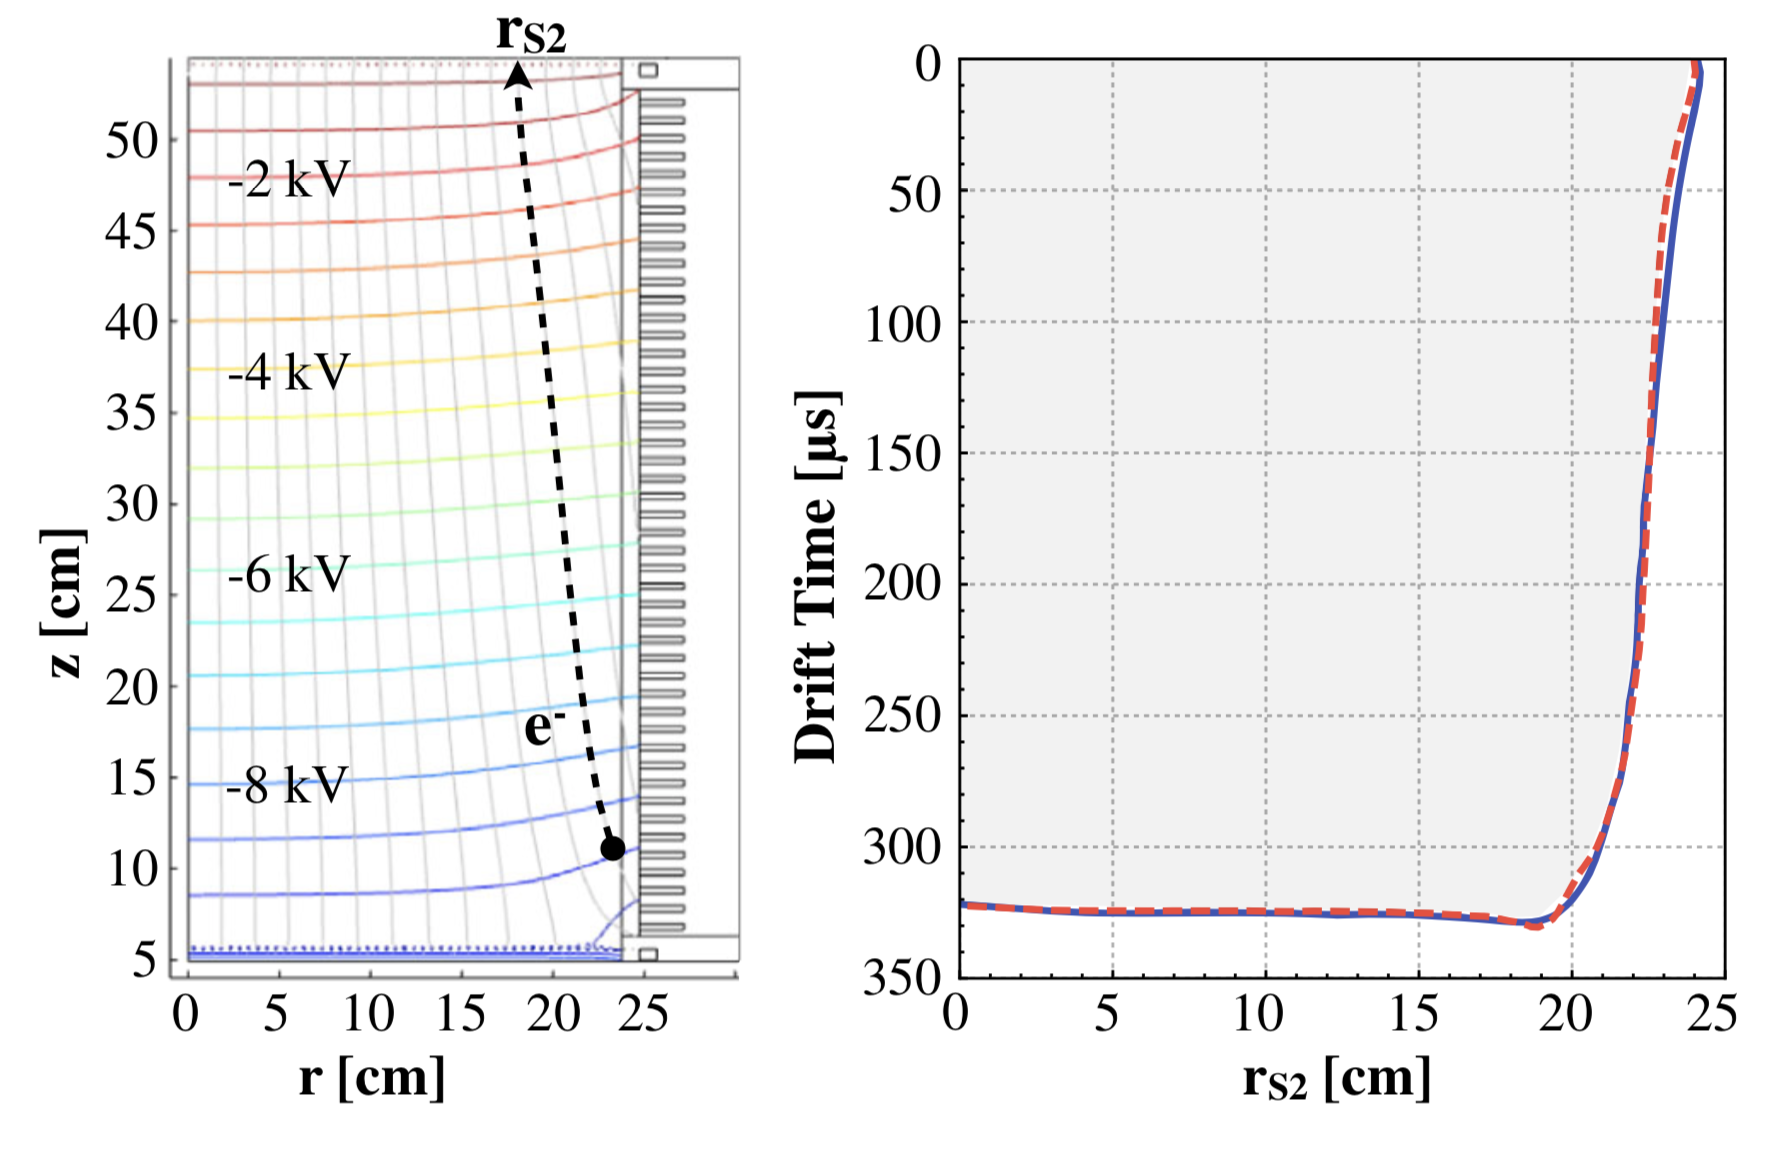
\includegraphics[width=.8\textwidth]{figures/lux/kr_pos1.png}
%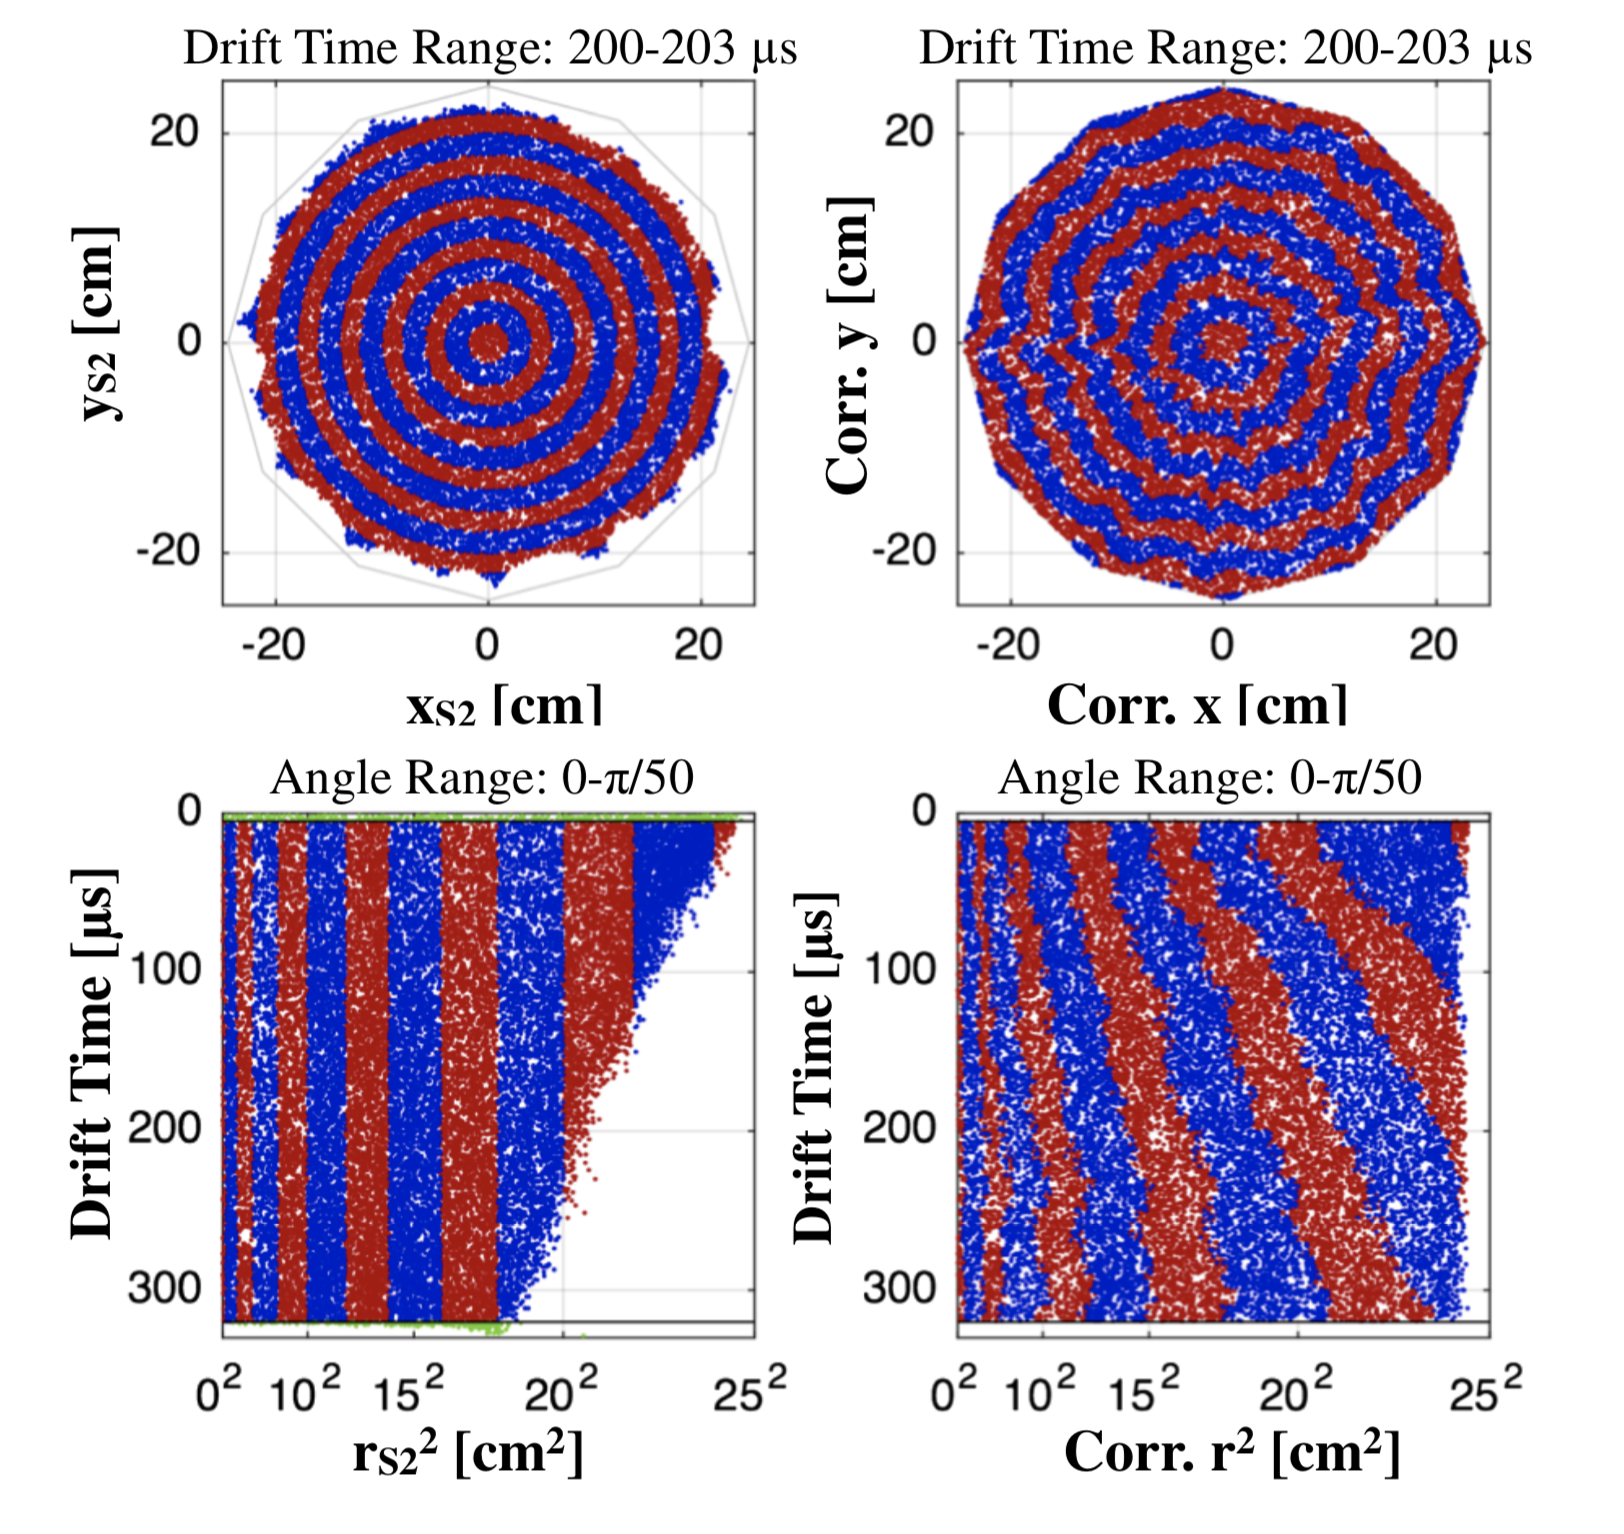
\includegraphics[width=\halffig]{figures/lux/kr_pos2.png}
\caption{ (Left) A simplified 2D COMSOL model showing electric field lines and equipotentials for the \ac{LUX} detector in Run03. A radially inward component is seen. (Right) The resulting edge S2 coordinates of a uniform distribution of electrons drifted under the electric field model is shown in solid blue. The edge S2 coordinates of from $^{83m}$Kr data is in dashed red; it is consistent with the field model prediction. Figure from \cite{LUXKr}}
\label{fig:kr_pos1}
\end{center}
\end{figure}

\begin{figure}[htbp]
\begin{center}
%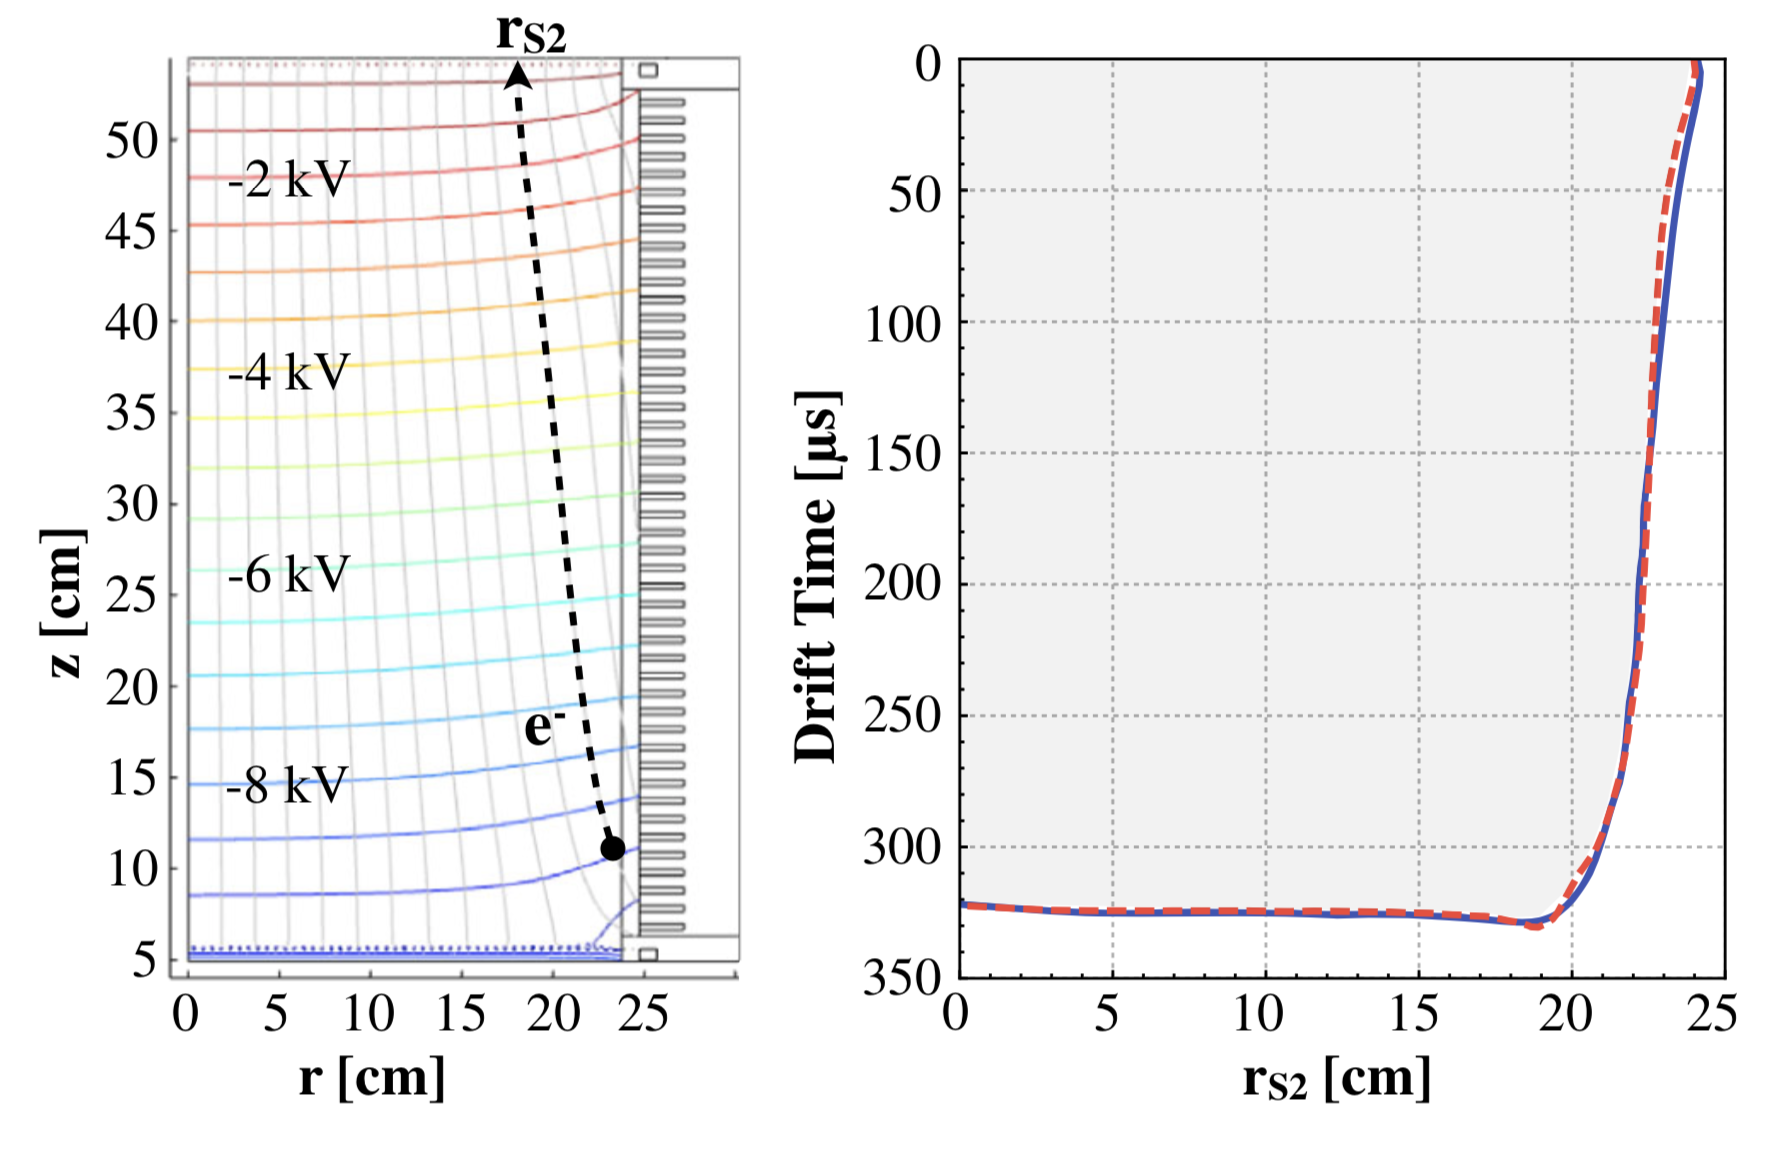
\includegraphics[width=\halffig]{figures/lux/kr_pos1.png}
\includegraphics[width=.8\textwidth]{figures/lux/kr_pos2.png}
\caption{ The effect of radial position mapping between S2 coordinates (left) and real coordinates (right). The top panels show a thin horizontal slice of the detector and the bottom panels show a thin vertical slide. The red and blue colors are to made the effect of the mapping visible. Note that squared radius in the bottom panels exaggerates the scale of the effect. Figure from \cite{LUXKr} }
\label{fig:kr_pos2}
\end{center}
\end{figure}

In addition to the small radial dependence, the electric fields illustrated in Figure~\ref{fig:kr_pos1} also vary in magnitude. The two decays of $^{83m}$Kr can be leveraged to directly probe the magnitude of the field, as they exhibit different field dependence. The ratio of S1a to S1b increases with field, and provides a measure the spatial dependence of the magnitude of the electric field. A highly variant electric field would affect recombination, and cause different light and charge yields at different positions in the detector, in turn affecting sensitivity. The fields measured via this method in Run03 were found to only cause corrections on the order of a percent and so no field-dependent corrections were applied \cite{LUXKr}. However, in Run04 the ratio technique was of central importance (see \cite{LUXCombinedExposure} \cite{LUXFields} \cite{LUXKr} for more detail). The result of the ratio method for measuring electric field magnitude is shown in Figure~\ref{fig:kr_3} for Run03 fields.

\begin{figure}[htbp]
\begin{center}
\includegraphics[width=0.69\textwidth]{figures/lux/kr_3.png}
\caption{Field map of Run03 produced by $^{83m}$Kr S1a:S1b ratio. Because only a fraction of $^{83m}$Kr produce separate S1a and S1b, the bins are large to accomidate reduced statistics. Figure from \cite{LUXKr} }
\label{fig:kr_3}
\end{center}
\end{figure}

\subsection{Tritium Beta Decay: Calibration of the ER Band and Yields}
In order to calibrate the \ac{ER} band of \ac{LUX} a $\beta$ source in the \ac{WIMP} energy range was needed. \ac{LUX} used a gaseous tritiated methane (CH$_{3}$T) source to deliver tritium uniformly into the active volume. Tritiated methane was chosen over the molecular tritium (T$_{2}$) because it does not adsorb onto surfaces like the smaller T$_{2}$ molecule and it does not interfere with charge transport in \ac{LXe} \cite{LUXTritium}. Tritium has a Q-value of 18.6~keV, but the spectrum peaks at 2.5~keV, with 64.2\% of the decays occurring in the \ac{WIMP} search energy range of 1 to 8~keV \cite{LUXTritium}. The half-life of tritium is 12.3~years, so efficient removal was essential. \ac{LUX} demonstrated that once deployed, CH$_{3}$T was removed with a 6~hour time constant, returning the detector back to acceptable \ac{WIMP} search rates. CH$_{3}$T was shipped to site in a bottle, mixed with purified xenon and released into the circulation system after the getter, to be swept into the inner volume. 

The tritium energy spectrum from data is shown with the theoretical energy spectrum convoluted with the detector energy resolution in Figure~\ref{fig:tritium1} (left). The ratio of the the two is shown in Figure~\ref{fig:tritium1} (right), demonstrating a 50\% effective energy threshold for \ac{ER} events at 1.24 $\pm$ 0.026~keV. The agreement between data and theory shows powerful support for the energy model E = W (S1/g$_{1}$ + S1/g$_{2}$). 

\begin{figure}[htbp]
\begin{center}
\includegraphics[width=\halffig]{figures/lux/lux_tritium1a.png}
\includegraphics[width=\halffig]{figures/lux/lux_tritium1b.png}
\caption{ (Left) Plot showing the theoretical tritium beta spectrum with the spectrum obtained from data, and residuals. (Right) The ratio of data to theory convoluted with the detector energy resolution. Figure from \cite{LUXTritium}}
\label{fig:tritium1}
\end{center}
\end{figure}

Tritium was also used to measure the light and charge yields over a wide energy range. Figure~\ref{fig:tritium3} (left) shows the detected number of quanta, $n_{\gamma}$ and $n_{e}$. Recall that is this is not necessarily the number of initial quanta $n_{ex}$ and $n_{ion}$ that are produced, as some number of $n_{ion}$ undergo recombination to produce additional scintillation photons.  Figure~\ref{fig:tritium3} (right) shows the effect that event energy has on recombination. For \ac{ER} events $n_{ex} / n_{ion} = 0.2$ is assumed to be constant \cite{LUXYieldsAndRecombination}, but the observed ratio $n_{\gamma} / n_{e}$ is clearly energy dependent.

\begin{figure}[htbp]
\begin{center}
\includegraphics[width=\halffig]{figures/lux/lux_tritium3a.png}
\includegraphics[width=\halffig]{figures/lux/lux_tritium3b.png}
\caption{ (Left) The measured quanta yields shown with lines of equal energy. (Right) A plot depicting the expected initial quanta yields, $N_{ion}$ and $N_{ex}$, compared with the measured yield of photons and electrons. The difference is causes by the energy dependence of recombination. Figure from \cite{LUXTritium}}
\label{fig:tritium3}
\end{center}
\end{figure}

Lastly, as is tritium was used to construct the \ac{ER} band (Figure~\ref{fig:tritium2} (left)), which is necessary for \ac{WIMP} search. The width of the \ac{ER} band is of significant interest, as it determines the nuclear recoil discrimination of the detector. The number of \ac{ER} events from the tritium calibration that occur below the nuclear recoil band mean is known as leakage fraction ($f$), and is shown as a function of energy in (Figure~\ref{fig:tritium2} (right)). The average \ac{ER} discrimination efficiency ($1-f$) for Run03 was 99.81\% $\pm$ 0.02\%(stat) $\pm$ 0.1\%(sys), where the systematic error comes from the error on $g_{1}$ and $g_{2}$. This measurement of discrimination efficiency relies on knowing the mean and width of the \ac{NR} band, which is discussed in the next section.

\begin{figure}[htbp]
\begin{center}
\includegraphics[width=\halffig]{figures/lux/lux_tritium2a.png}
\includegraphics[width=\halffig]{figures/lux/lux_tritium2b.png}
\caption{ (Left) The \ac{ER} band for in \ac{WIMP} search energy range obtained from the tritium calibration. (Right) Leakage fraction of \ac{ER} events below the \ac{NR} mean in the \ac{WIMP} search energy range. Knowledge of the \ac{NR} band comes from the DD calibration detailed in Section~\ref{sec:DD}. Figure from \cite{LUXTritium}}
\label{fig:tritium2}
\end{center}
\end{figure}

\subsection{Low-energy nuclear recoils from Deuterium-Deuterium (DD) Neutrons: NR Band and Yields}
\label{sec:DD}
A \ac{DD} generator was used to calibrate the \ac{NR} response and signal yields for \ac{LUX} in the \ac{WIMP} search energy range. A photo and diagram of the calibration scheme are shown in Figure~\ref{fig:dd_gen}. Following Run03, \ac{LUX} employed the \ac{DD} generator to deliver a collimated beam of 2.45~MeV neutrons into the \ac{TPC}. As Figure~\ref{fig:dd_gen} shows, the generator was positioned outside the water tank, but when aligned with the neutron conduit (a \ac{PVC} tube of air), deposited neutrons into the \ac{LXe} space. The \ac{DD} calibration leverages known kinematics of neutron scattering, the known incoming neutron energies, and the known detector gains $g_{1}$ and $g_{2}$ to develop a complete characterization of low-engergy \ac{NR} in \ac{LUX}. The method is summarized here, but details are available in \cite{LUXDD}.

\begin{figure}[htbp]
\begin{center}
\includegraphics[width=\textwidth]{figures/lux/lux_ddgenerator.png}
\caption{(Right) Photo of the water tank interior showing the neutron conduit, which is raised during \ac{DD} calibration. (Left) Diagram of the \ac{DD} generator and water tank neutron conduit during \ac{DD} operation. Figure courtesy of E. Pease.}
\label{fig:dd_gen}
\end{center}
\end{figure}

First, charge yield was derived from a population of multiscatter events: those with one S1 (the S1s are merged due to simultaneous collection of S1s) and two S2s (separated in space and z-position/drift time). Neutron scattering kinematics allow for the reconstruction of energy at the first scatter site, so the unknown first S1 is not needed to ascertain the energy deposition. The charge yield is then obtained from the first S2 and the energy of the first scatter from kinematics. 

Once the charge yield was obtained, a population of single scatter events was collected: one S1 and one S2. These events were from neutrons that scattered once the detector, and then exited. Here, the second scatter is not available to kinematically reconstruct energy, so instead the charge yield is employed to infer the energy of the single scatter. The light yield is then obtained from the S1 and the energy deposition inferred from charge yield. 

It should be noted that though the \ac{DD} generator produced monoenergetic neutrons of initial energy $E_{i}$, the energy deposited $E_{d}$ by a neutron scatter is

\begin{equation}
E_{d} = E_{i} \frac{m_{n} M_{Xe}}{m_{n} + M_{Xe}} sin^{2}\theta_{CM}
\end{equation}

Where $m_{n}$ in the neutron mass, $M_{Xe}$ is the xenon mass, and $\theta_{CM}$ is the scattering angle relative to the neutron conduit in the center of mass frame. The deposited energy, $E_{d}$ then covers a range of energies, allowing for calibration of the \ac{NR} band and yields over a range of energies. After determination of the light yield, the single scatter events were used to construct the \ac{NR} band in Figure~\ref{fig:lux_nrband}.

\begin{figure}[htbp]
\begin{center}
\includegraphics[width=\textwidth]{figures/lux/lux_nrband.png}
\caption{Calibration showing the \ac{NR} band mean and width from the \ac{DD} calibration. Figure from \cite{LUXDD}}
\label{fig:lux_nrband}
\end{center}
\end{figure}

\subsection{Power of LUX Calibrations}
Although this thesis is concerned mainly with a search for \ac{LIP}s, it should be noted that the extensive \ac{LUX} calibrations allowed for excellent understanding of the detector, resulting in a world-leading \ac{WIMP} limit. In particular, the \ac{DD} calibration (carried out after Run03) yielded a much better understanding of the \ac{NR} band and yields, and therefore detector thresholds, than the initial \ac{AmBe} neutron calibration which was carried out in the early days of \ac{LUX}. The power of the \ac{DD} calibration can be seen in the difference between the first \ac{LUX} result \cite{LUXFirstResults} and the Run03 re-analysis \cite{LUXReanalysis} shown in Figure~\ref{fig:lux_reanalysis}. In particular, improved knowledge of the scintillation yields allowed a re-analysis threshold down to 1.1~keV$_{nr}$ where the initial \ac{WIMP} search adopted the more conservative threshold of 3.0~keV$_{nr}$. This improvement allowed \ac{LUX} to exclude new spin-independent parameter space below a \ac{WIMP} mass of 10~GeV. 


\begin{figure}[htbp]
\begin{center}
\includegraphics[width=\textwidth]{figures/lux/lux_reanalysis.png}
\caption{Improved spin-independent \ac{WIMP} limit of the Run03 exposure following the \ac{DD} calibration of \ac{LUX}. The first Run03 limit is the gray line labelled ``LUX~2014'', the improved Run03 observed limit is the black line labelled ``This Result''.  Figure from \cite{LUXReanalysis}}
\label{fig:lux_reanalysis}
\end{center}
\end{figure}




%*****************************************
%*****************************************
%*****************************************
%*****************************************
%*****************************************

%************************************************
\chapter{Lightly Ionizing Particle Search}

\label{ch:lips} % $\mathbb{ZNR}$
%************************************************

\begin{flushright}{\slshape    
   And all this science I don't understand, \\
     It's just my job five days a week } \\ \medskip
    --- {Elton John \textit{Rocket Man, 1972}}
\end{flushright}



\section{Modeling LIP Interaction}
\subsection{Collision Cross Section}
A \ac{LIP} interacting in the \ac{LXe} volume loses energy via interaction with electrons.  To model \ac{LIP}s in \ac{LUX}, the expression of interest is the collision cross section \ac{CCS}. The differential \ac{CCS} describes the energy lost to electrons in a single collision for incident energy of the LIP. For particles with charge $ze$ and mass M heaver than the electron mass,$ m_{e}$ ( ``heavy'' particles), the Rutherford cross section is a familiar differential \ac{CCS} \cite{PDG}:

\begin{equation}
\label{ruth}
\frac{d\sigma_{R}}{dE} = \frac{2\pi r_{e}^{2} c^{2} z^{2}}{\beta^{2}} \frac{1-\beta^{2} E/ T_{max}}{E^{2}}
\end{equation}

where $r_{e}$ is the classical electron radius, $E$ is the energy loss of incoming particle, $\beta = v/c$ of the incoming particle, and $T_{max}$ is the maximum energy transfer possible in a single collision:

\begin{equation}
\label{Tmax}
T_{max} = \frac{ 2m_{2}c^{2} \beta^{2} \gamma^{2}}{1 + 2\gamma m_{2} / M + (m_{e}/M)^{2}}
\end{equation}

Often the expression $T_{max} ~ 2m_{e}c^{2} \beta^{2}\gamma^{2}$ for $2\gamma m_{2} / M<< 1$ is used implicitly, or is referred to as the ``low energy approximation'' in older texts. The Rutherford cross section is a good starting point, but it describes the ``hard interaction'' or head-on, billiard-ball type collision of a particle interacting with free electrons. Real electrons are bound in atoms, and an incident particle can undergo ``soft interactions'', in which virtual photons are exchanged. When the virtual photon matches the energy of electron orbitals of the target material, there are resonances in the \ac{CCS}. The energy transfer, $E$, must also be finite in real atoms, where the dielectric properties modify the electromagnetic field of a moving charged particle and limit the growth of the cross section. This real-world behavior is described by a correction factor $B(E)$, also sometimes called an ``inelastic form factor'' \cite{PDG}:

\begin{equation}
\label{totalccs}
\frac{d\sigma_{CCS}}{dE} = \frac{d\sigma_{R}}{dE} B(E)
\end{equation}

Various attempts, spanning a better half of the last century, have been made to take into account the real-world behavior of electrons bound in matter. Some of these can be found in [cite 18,27, 41-43 papers from Bichsel]. More well-known contributions are those of Bethe and Fano. In 1930, Bethe derived a cross section doubly differential in energy loss and momentum transfer using the first Born approximation for scattering on free atoms \cite{Bethe:1930}. In 1963, Fano extended the method to describe atoms in solids \cite{Fano:1963}. Combining their two methods yields the Bethe-Fano cross-section, which has undergone much study and by our current understanding has been verified to be close to reality \cite{Bichsel:2006}. There is another method, called the \ac{PAI} model, that is easier to calculate than the Bethe-Fano cross section, and approximates the Bethe-Fano calculation very closely. This thesis uses the \ac{PAI} model as a base, building the full signal model for \ac{LIP}s interacting in the \ac{LUX} detector. 

\subsection{Photo Absorption Ionization Model for Charge Particle Energy Loss}
The \ac{PAI} model is also sometimes known as the \ac{FVP} or Weis�cker-Williams approximation. A full description of the \ac{PAI} model is described in detail in \cite{AllisonCobb:1980}. The complex dielectric constant $\epsilon = \epsilon_{1} + i \epsilon_{2}$ can be thought of a encoding all the information about a medium. The real part $\epsilon_{1}$ describes the polarization of the material and imaginary part $\epsilon_{2}$ describes the absorptive properties. Typically both $\epsilon_{1}$ and $\epsilon_{2}$ are thought of as functions of $\omega$, or incident photon energy. So $\epsilon(\omega)  = \epsilon_{1}(\omega) + i \epsilon_{2}(\omega) $. This description is limited to free photons, but we desire to describe inelastic collisions as well. So $\epsilon(k, \omega)$, a generalized dielectric constant, is introduced to describe momentum transfer $k$ to atomic electrons. The generalized dielectric constant $\epsilon(k, \omega)$ can be related to atomic matrix elements, and if desired, calculated completely and tediously. However, the \ac{PAI} model allows us to avoid these tedious calculations by making specific approximations, which, when taken together, define the \ac{PAI} model itself. 

In particular, the \ac{PAI} model approximates $\epsilon_{2}(k, \omega)$ by noting that typically, the momentum $k$ transferred to an electron is much less than the energy transfer $\omega$. 



\subsection{Straggling}
\subsection{Energy Resolution in LUX}
\subsection{Position Resolution in LUX}

\section{LIP Search}
\subsection{LUX Run03 Conditions}

\section{LIP Search Analysis}
\subsection{Energy Consistency}
\subsection{Track Linearity Criteria}
\subsection{Background Rejection}
\subsection{Muons}
\subsection{Gammas}
\subsection{Electron Trains?}

\section{Result: Vertical Flux Limit}


%*****************************************
%*****************************************
%*****************************************
%*****************************************
%*****************************************


\cleardoublepage % Empty page before the start of the next part
%----------------------------------------------------------------------------------------
\ctparttext{This section describes research with a small test bed at Lawrence Berkeley National Lab. The details of test bed construction and operation are discussed, with particular attention to construction of high voltage feed throughs. Two studies affecting the sensitivity of future \acs{LXe} \acs{TPC}s are described. One study investigates the solubility of radon daughters, and another furthers understanding of delayed electron noise phenomena.} % Text on the Part 2 page describing the content in Part 2

\part{Little Science}
\label{part:labwork}

%************************************************
\chapter{Research and Development Testbed For Future Liquid Xenon TPCs}

\label{ch:testbed} % $\mathbb{ZNR}$
%************************************************

\begin{flushright}{\slshape    
  All systems go, are you sure? } \\ \medskip
    --- {Peter Schilling \textit{Major Tom, 1969}}
\end{flushright}


A small test bed was built at Lawrence Berkeley National Laboratory to study various detector effects facing large \ac{LXe} \ac{TPC}s. The test bed was built and instrumented over the course of about two years, from 2015 through 2016. This chapter describes some of the details of that instrumentation.

\section{Test Bed Apparatus Overview}

\begin{figure}[htbp]
\begin{center}
\includegraphics[width=\textwidth]{figures/testbed/apparatus.jpg}
\caption{Large scale view of the experimental apparatus showing key parts. The \acs{CF} tower extent is indicated with a dotted line; this whole tower is also part of the inner xenon space.}
\label{fig:apparatus}
\end{center}
\end{figure}

A large-scale overview of the testbed is shown in Figure~\ref{fig:apparatus}, and a diagram of the inner experimental vessel is shown in Figure~\ref{fig:internals}. The experimental apparatus consisted of an inner vessel, a vacuum outer vessel, and a xenon circulation system. The inner vessel was a \ac{SS} canister, topped with a 2.75~in Conflat-adaptable tower that allowed space for instrumentation cabling and \ac{HV} feedthroughs. The inner vessel was offset below a 7.09~in ISO K flange, which held the (removable) vacuum outer vessel in place. Several Mini-CF ports were welded to the ISO K flange for instrumentation cabling. A \ac{LN} reservoir was thermally connected to the cold-head. A half-inch pipe opened into the bottom of the reservoir, which was offset above the ISO-K flange; this allowed \ac{LN} to flow into the pipe. The bottom of the pipe was connected to the cold-head via braided copper wire. A Swagelock vacuum fitting sealed the lower-half of the pipe into the outer vacuum space.

The inner vessel contained the \ac{TPC}. A \ac{PTFE} housing cylinder fastened a \ac{PMT} in place. Above the \ac{PTFE} housing, a series of interlocking \ac{PTFE} rings held strung wire grids and a segmented anode in place. During data taking, the entire \ac{PMT} and housing were immersed in \ac{LXe}. The liquid level was chosen depending on the experiment being performed, and was approximated by the S2 width. In some cases, the \ac{TPC} was ``overfilled'' by allowing the liquid level to rise above the anode. The segmented anode was instrumented with charge amplifiers for direct charge readout. When the \ac{TPC} was overfilled, the charge amplifiers detected the ionization electrons directly from the liquid. During typical dual phase \ac{TPC} operation, the charge amplifiers provided a secondary measurement of the ionization electrons in addition to S2. Two typical arrangements of the inner vessel are shown in Figure~\ref{fig:internals}.

\begin{figure}[htbp]
\begin{center}
\includegraphics[width=\textwidth]{figures/testbed/internals_1and2.png}
%\includegraphics[width=\halffig]{figures/testbed/internals1.png}
%\includegraphics[width=\halffig]{figures/testbed/internals2.png}
\caption{Diagrams of two often used internal arrangements. The configuration (left) has both a drift and extraction region. The configuration (right) is ``extraction region only''. The blue region with the wavy line indicates the liquid level. }
\label{fig:internals}
\end{center}
\end{figure}


\section{Circulation System}
The xenon circulation system in shown in Figure~\ref{fig:circ}. A stainless steel capillary extending into the liquid drew xenon from the inner vessel during operation to be purified. Purified xenon that was returned to the vessel was directed into the liquid via a \ac{PTFE} tube so it could condense quickly. A gas purge from a \ac{CF} tower above the inner vessel could be opened to continually renew the gas column. 

\begin{figure}[htbp]
\begin{center}
\includegraphics[width=\textwidth]{figures/testbed/full_pid.png}
\caption{Pumping and instrumentation diagram of the test bed. Special symbols are labelled in the diagram, see key for other symbols. For readability, all gauges are not shown.}
\label{fig:circ}
\end{center}
\end{figure}


\section{Slow Control}
The slow control for the test bed consists of a few monitoring variables such as temperature and pressure and a voltage supply that switches resistive heaters on/off. The inner experimental vessel was instrumented with two platinum \ac{RTD}s to monitor temperature and a capacitance manometer to monitor pressure. A flow meter in the circulation line determined the flow rate of xenon as it passed through the getter and returned to the inner vessel. These four variables were read using Omega i-series digital panel meters to provide a real-time display; two points of calibration were provided to the digital panel meters to translate voltage to human-readable pressure, temperature, etc. In addition, two 25~$\Omega$ resistors are mounted, in parallel, on the cold-head. Supplying voltage to these resistors raised the temperature of the cold-head and decreased the cooling power delivered by the liquid nitrogen bath; the voltage supplied to the heaters was also recorded, but not shown with digital panel meters. The voltages for the monitoring variables and the heater voltages were fed into a USB Device from Measurement Computing, which interfaces with a computer. A slow control script on a lab computer recorded the monitoring variables and heater voltages. The script also determined if power should be supplied to the heaters and if text message and e-mail alarms should be sent for a variable out of expected range. A basic schematic of the slow control is shown in Figure~\ref{fig:sc}.

\begin{figure}[htbp]
\begin{center}
\includegraphics[width=\textwidth]{figures/testbed/slow_control.png}
\caption{A diagram showing components of the slow control.}
\label{fig:sc}
\end{center}
\end{figure}


\section{PMT}
The test bed was instrumented with a Hammamatsu R8778 \ac{PMT}, the same model of \ac{PMT} used in \ac{LUX}. A \ac{LUX} \ac{PMT} base was used and an \ac{LZ} \ac{PMT} base was tested. The radon daughters study presented in Chapter~\ref{ch:radon} exclusively used the \ac{LUX} \ac{PMT} base; the electron trains studies presented in Chapter~\ref{ch:etrains} first used the \ac{LUX} base, and later used the \ac{LZ} base. Various shaping amplifiers were used when digitizing the \ac{PMT} over the course of these studies because the 8~ns sampling interval of the data acquisition was subject to aliasing the fast-rising alpha S1 signals.



\section{Charge Amplifiers}
The \ac{TPC} diagram in Figure~\ref{fig:internals} includes a segmented anode, the largest segment of which is held at ground. The anode is pictured in Figure~\ref{fig:anode} and relevant dimensions are included in Table~\ref{T:anode_segs}.

\begin{figure}[htbp]
\begin{center}
\includegraphics[width=\halffig]{figures/testbed/anode.png}
\includegraphics[width=\halffig]{figures/testbed/anode2.png}
\caption{(left) Segmented anode showing the xenon-facing anode segments. The innermost segment is referred to as the ``bullseye'', the next is called the ``inner ring'' and the last is called the ``outer ring''. The largest segment on the anode was not instrumented with charge amplifiers and was held at ground. (right) The wires on the top of the anode which lead to the charge amplifiers.}
\label{fig:anode}
\end{center}
\end{figure}

\begin{table}[ht]
\centering
\begin{tabular}{rcccc}
\hline
%& \multicolumn{3}{c}{\bf Datasets}\\[-5pt]
 Anode Segments & 1 & 2 & 3 & Full \\
\hline
Radius (mm) & 3  & 6 & 9 & 24 \\
Cumulative Area (mm$^{2}$) & 28 &  113 & 255 & 1810 \\
\end{tabular}
\caption{Dimensions of the of the anode segments. 1 refers to the inner-most segment or ``bullseye'', 2 refers to the inner ring, 3 to the outer ring and full to the entire anode, which includes inactive area that is not instrumented with charge amplifiers.}
\label{T:anode_segs}
\end{table}

The segmented anode was instrumented with three CR-110 charge amplifiers from Cremat (Figure~\ref{fig:cr110}). The raw charge amplifier signals were each fed into a CR-160-R7 shaper evaluation board, also from Cremat. The evaluation board houses two more modules: one CR-200-X shaping amplifier and one CR-110 baseline restorer. The CR-200-X shaping amplifier is an X-$\mu$s gaussian shaping amplifier; it was determined that 1~$\mu$s was most appropriate for the test bed signals, based on the size of the gas gap and the expected event rat. 

\begin{figure}[htbp]
\begin{center}
\includegraphics[width=4in]{figures/testbed/cr110.png}
\caption{A picture of the CR-110 charge amplifier from the manufacturer's data sheet, shown with an equivalent circuit diagram.}
\label{fig:cr110}
\end{center}
\end{figure}

The shaper evaluation board produced gaussian pulses from raw charge signals as shown in Figure~\ref{fig:shaper}.

\begin{figure}[htbp]
\begin{center}
\includegraphics[width=4in]{figures/testbed/charge_amp_shaper.jpg}
\caption{A raw (cyan) and shaped (yellow) charge amp signal taken in -100C gaseous xenon, with the radon source plumbed in. The \acs{PMT} signal is visible in blue and the \acs{NIM} trigger signal is in magenta.}
\label{fig:shaper}
\end{center}
\end{figure}

The charge amplifiers were originally placed inside the experimental vessel, mounted directly on the segmented anode. The functionality of the CR-110 units in \ac{LXe} conditions did not deviate from manufacturer's specifications\footnote{A test was done in a cryogenic fridge to ensure the behavior of the charge amps did not deviate when they were kept at -100~C. There was no change in pulse height (for a fixed input charge), or rise and decay times of the raw signals. This test was not possible in-situ, and so excludes the noise behavior described below, because the manufacturer's test board (CR-150-R5 evaluation board) was necessary to inject charge (via a square wave to an on-board 1~pF capacitor) into the amplifiers.}, however it was found that the units generated enough heat to create a perpetual gas layer under the anode. In general this is not an issue, but for the purpose of the intended absolute electron extraction efficiency measurement, overfilling the \ac{TPC} and using the charge amplifiers as a direct read-out of electrons in the liquid was required. The charge amplifiers were moved to the outer vessel space, surrounded by a small Faraday cage made of copper mesh. See Figure~\ref{fig:chargeamp_mount} for the charge amplifier mounting configurations.

 \begin{figure}[htbp]
\begin{center}
\includegraphics[height=2.5in, keepaspectratio]{figures/testbed/chargeamp_mount1.jpg}
\includegraphics[height=2.5in, keepaspectratio]{figures/testbed/chargeamp_mount2.jpg}
\caption{(left) original mounting of CR-110 charge amplifiers inside the experimental vessel. (right) Mounting in the outer vacuum reduced heat load on the \acs{TPC}. In the outer vessel, the charge amplifiers were surrounded by a Faraday cage constructed from copper mesh to reduce noise.}
\label{fig:chargeamp_mount}
\end{center}
\end{figure}

\subsection{Charge Amplifier Noise Behavior}
Charge amplifiers have baseline RMS noise proportional to the attached capacitance. Figure~\ref{fig:rms} shows the RMS noise of a CR-110 unit attached to different lengths of BNC cable. The longer the cable, the higher the RMS noise. \ac{TPC}s are essentially capacitors, and when filled with \ac{LXe} have a higher capacitance than when the detector is at vacuum. The capacitance of large \ac{LXe} \ac{TPC}s like \ac{LUX} prohibit the use of charge amplifiers for direct readout of the S2 electrons because the RMS noise would swamp the signal. 

\begin{figure}[htbp]
\begin{center}
\includegraphics[width=3in]{figures/testbed/rms.png}
\caption{Different lengths of BNC cable attached to a CR-110 test board to show the RMS noise relationship to input capacitance. Two equal length segments (calculated to be 33.3~pF) were observed to have slightly different properties.}
\label{fig:rms}
\end{center}
\end{figure}

Charge amplifiers also respond to acoustics; that is, they are susceptible to microphonic noise. Tapping a finger near a charge amplifier will show as a baseline-jumping response on an oscilloscope. This additional source of noise makes \ac{LXe} \ac{TPC}s challenging places to use charge amplifiers for signal readout because any bubbles in the \ac{LXe} create microphonic signals which the charge amplifiers pick up. By design, dual phase \ac{LXe} \ac{TPC}s are operated near the xenon liquid-gas boundary so the formation and dissipation of gas bubbles in the liquid is likely. Additional sources of acoustic noise like circulation of xenon into the experimental vessel also produce visible responses in charge amplifiers. The difference in micro-acoustic noise environments (gas phase but with/without the circulation pump) is illustrated in Figure~\ref{fig:amp_noise}. The baseline restorer can be seen functioning on the gaussian shaped and amplified signals, but the raw charge signals are subject to baseline wandering (Figure~\ref{fig:amp_noise2}). Figure~\ref{fig:amp_noise2} was taken in a liquid environment during filling, so the effect of bubbles, pressure changes, and other vibrations are visible. 

 \begin{figure}[htbp]
\begin{center}
\includegraphics[width = 0.32\textwidth, keepaspectratio]{figures/testbed/circ_off.png}
\includegraphics[width = 0.32\textwidth, keepaspectratio]{figures/testbed/circ_noise.png}
\includegraphics[width = 0.32\textwidth, keepaspectratio]{figures/testbed/circ_noise_zoom.png}
\caption{left) Event showing charge amp with detector -100~C, 1.5~bar, gas only (time scale 1.00~ms/div). (middle) Effect of circulation pump on charge amp is to cause 500~Hz oscillation noise (-100~C, 1.5~bar, gas only (time scale 1.00~ms/div)). (right) Same event as (middle), but zoomed-in time scale (10.0~$\mu$s/div). In all figures, cyan is the raw charge signal (1~mV/div), yellow is the shaped charge (100~mV/div), blue is the \acs{PMT} (10~mV/div) and magenta is the \acs{NIM} trigger (100~mV/div).}
\label{fig:amp_noise}
\end{center}
\end{figure}

 \begin{figure}[htbp]
\begin{center}
\includegraphics[width = \halffig, keepaspectratio]{figures/testbed/baseline_wander.jpg}
\includegraphics[width = \halffig, keepaspectratio]{figures/testbed/baseline_wander_zoom.jpg}
\caption{An event with the detector at  -100~C, 1.5~bar, with liquid condensed to a level between extraction grid and anode. In both figures, cyan is the raw charge signal (1~mV/div), yellow is the shaped charge (100~mV/div), blue is the \acs{PMT} (10~mV/div) and magenta is the \acs{NIM} trigger (100~mV/div). (left) Scope trace showing a long time view the raw and shaped charge amplifier signals (time scale 1.0~ms/div). (right) Scope trace showing the same event, but zoomed in (10.0~$\mu$s/div). The baseline restorer on the shaped charge signal allowed it to be used as a trigger.}
\label{fig:amp_noise2}
\end{center}
\end{figure}


As \ac{TPC}s are effectively large parallel plate capacitors, any transients coupling to the ``\ac{TPC} capacitor" may be picked up by the charge amplifiers. In particular, instabilities in the \ac{HV} chain induce a current in the \ac{TPC} capacitor that is picked up by the charge amps. Instabilities in \ac{HV} can come from many places. It was observed that for the characteristic capacitance and impedance of the the test bed, partial breakdowns in a length of RG60 cabling caused a disruption in the functionality of the charge amplifiers. It was also found that a standard laboratory \ac{HV} supply, a Glassman 20~kV negative polarity unit, created pick-up in the charge amplifiers (see Figure~\ref{fig:pickup_noise}).  

 \begin{figure}[htbp]
\begin{center}
\includegraphics[width = 0.49\textwidth, keepaspectratio]{figures/testbed/glassman_noise.png}
\includegraphics[width = 0.49\textwidth, keepaspectratio]{figures/testbed/partial_breakdown_pickup.png}
\caption{(left) 50~kHz periodic noise from the Glassman 20~kV negative polarity voltage supply. (right) Partial breakdown in RG60 cable as picked up by charge amplifiers. In both figures, the time scale is 10.0~$\mu$s/div and the voltage scale is 2.00~mV/div.}
\label{fig:pickup_noise}
\end{center}
\end{figure}



%\subsection{\ac{PMT} Saturation}



\section{Data Acquisition and Processing}
Data were acquired with a Picoscope 5000a, a USB-compatible ``oscilloscope." The open source pico-python Python library was used to write voltage records of \ac{PMT} and charge signals to ROOT files, which were opened later for reprocessing into reduced quantities such as pulse area or pulse height. The Picoscope was run as a 14~bit ADC with 125~MHz (8~ns) sampling. For special cases, when only one channel was desired, it was possible to increase the sampling rate to 500~MHZ (2~ns). The manufacturer guide states that the Picoscope can operate in block mode, which uses on-board memory to store events and transfers them to disk only when the on-board memory buffer is full. Block mode is generally preferable to writing each event to disk as it is acquired because the overhead time for USB communication between the Picoscope and write time is only executed once, and so the dead time per event is smaller. However, the block mode capabilities were found to not function and so single event acquisition was used.

\subsection{Estimating Picoscope Dead Time}
Each event was written to disk as it was acquired, which led to a large dead time percentage. The manufacturer provided no information about dead time, but in general, dead times can be estimated in lab using the following method. Trigger the DAQ externally with, e.g., a square wave. Vary the rate of the external trigger, counting how many events are actually recorded by the DAQ in 1 minute. The number of events actually recorded gives the record rate. The record rate will level off at high external trigger rates because it is limited by transfer speed, write time, etc. Subtracting the actual event length from the real total time it takes to record an event gives the dead time per event. When estimating dead times, use the same conditions in data taking, e.g. if 4 channels are used for real data taking, use 4 channels when measuring the record rate. The dead time per acquisition is then the number of events in the acquisition multiplied by the dead time per event. This method is illustrated in Figure~\ref{fig:deadtime}. Such a dead time estimate is used in Chapter~\ref{ch:radon} to calculate the rate in Bq of radon daughters observed.

 \begin{figure}[htbp]
\begin{center}
\includegraphics[width =\textwidth ]{figures/testbed/deadtime_plot.png}
\includegraphics[width =\textwidth]{figures/testbed/deadtime_math.png}
\caption{(top) Laboratory method to find the maximum \acs{DAQ} record time time. (bottom) Calculating dead time from maximum record rate.}
\label{fig:deadtime}
\end{center}
\end{figure}


\subsection{PMT Signal Processing}
A simple pulse finder was written in Python. Instead of searching for pulses left-to-right along a signal trace, the algorithm found the maximum of the trace, and then searched left and right until the trace went below a threshold. After these edges were identified, the trace was set to zero for the duration of the pulse, and then the next-tallest pulse was sought. Pulses were found until there were no more, or the number found was equal to some user-defined number of pulses. Thus, pulse starts and stops were acquired for each \ac{PMT} trace. These pulse starts and stops were then used to calculate useful \ac{RQ}s such as pulse area, width, prompt fraction, etc. S1 and S2 identification was done later, based on these \ac{RQ}s. The definitions of S1, S2, and other high-level \ac{PMT} \ac{RQ}s were specific to the state of the test bed hardware, which was typically changed on a weekly basis during development. A stable data processing framework was not maintained. 

\subsection{Charge Amplifier Signal Processing}
\label{sec:charge_amp_processing}
The shaped charge amplifier signals were used primarily as a trigger throughout the studies in Chapter~\ref{ch:radon} and Chapter~\ref{ch:etrains}. They were originally acquired and implemented because the raw charge signals were small and difficult to process. This was due to field strength, purity, and grid transparency; these issues are described in more detail in Chapter~\ref{ch:etrains}, but were all essentially solved by removing the grid to produce an ``extraction region only'' configuration (Figure~\ref{fig:internals} (right)). Various methods were explored to process the raw signals into the relevant charge \ac{RQ}: step height (mV), which could then be translated to charge (Coulombs, then number of electrons) per the manufacturer's specifications. For small, raw charge signals a fit function was found to out-perform a simple step algorithm; for larger raw signals the step algorithm was fast and robust. Both methods are illustrated below, the fit function in Figure~\ref{fig:charge_fit} and the step algorithm in Figure~\ref{fig:charge_algorithm}. 

The fit function was a piece-wise defined linear function plus a falling exponential. The linear function was defined to be zero before some offset time $t_{o}$, and after the offset time plus rise time of the charge trace ($t_{o} + t_{r}$). The exponential was zero before $t_{o} + t_{r}$, and the two functions had equal values at $t_{o} + t_{r}$. 

The step algorithm produces a new trace with peak instead of a step by averaging a user-defined number of samples, $n_{s}$, of the original charge amp voltage trace from $[i+n_{s},i+2n_{s}]$ and subtracting the average of the waveform from a previous section, $[i,i+n_{s}]$. If $n_{s}$ is chosen to be exactly the rise time of the trace, then the maximum of the new trace is equal to the step height. See Figure~\ref{fig:nsamp_choice} for examples of two different choices of $n_{s}$. In practice, it is difficult to choose $n_{s}$ perfectly because noise plays a large role; it was easier instead to find the peak of the new trace to locate the approximate step position of the original trace based on $n_{s}$, and take the average of several samples as the step height (Figure~\ref{fig:charge_algorithm}). That is, if $n_{p}$ is the location of the peak after the step-finding algorithm, the approximate location of the step is $n_{p} + 2n_{s}$. 

 \begin{figure}[htbp]
\begin{center}
\includegraphics[width =\textwidth ]{figures/testbed/charge_fit.png}
\caption{Fitting the charge traces with a piece-wise defined linear rise and exponential fall. 1 sample is 8~ns.}
\label{fig:charge_fit}
\end{center}
\end{figure}

 \begin{figure}[htbp]
\begin{center}
\includegraphics[width =\halffig ]{figures/testbed/figure_q20.png}
\includegraphics[width =\halffig ]{figures/testbed/figure_q50.png}
\caption{The step-finding algorithm shown with a choice of 20 samples averaged (left) and with 50 samples averaged (right). If $n_{s}$ is chosen to be the rise time of the pulse, the height of the output waveform is the height of the step. These step algorithms actually include an offset, $n_{o}=1000$, so the averages are taken from $[i+n_{o}+n_{s},i+n_{o}+2n_{s}]$ and $[i+n_{o},i+n_{o}+n_{s}]$. Alternatively, a smaller number can be chosen for $n_{s}$, and the location of the maximum of the output waveform can be used to find the location of the top of the step (shown in Figure~\ref{fig:charge_algorithm}). 1 sample is 8~ns. }
\label{fig:nsamp_choice}
\end{center}
\end{figure}

 \begin{figure}[htbp]
\begin{center}
\includegraphics[width =\textwidth ]{figures/testbed/charge_algorithm.png}
\caption{The location of the top of the step can be robustly found from the location of maximum of the step-finding algorithm. Some number of samples at the top of the step can be averaged to give the step height. 1 sample is 8~ns. This particular example uses $n_{s}=20$. The step-finding algorithm is calculated with an offset, $n_{o}=1000$, so the averages are taken from $[i+n_{o}+n_{s},i+n_{o}+2n_{s}]$ and $[i+n_{o},i+n_{o}+n_{s}]$. If the peak location (red peak) is $n_{p}$, then the approximate location of the step is $n_{p} + n_{o} + 2n_{s}$, and some number of samples of the original trace (50 samples shown in green) can be averaged to give the step height. }
\label{fig:charge_algorithm}
\end{center}
\end{figure}


Another source of charge amplifier noise is the Shockley-Ramo effect. The Shockley-Ramo effect refers to the Shockley-Ramo theorem, which says that the instantaneous current $i$ and charge $Q$ induced on a given electrode due to the motion of a charge is \cite{He2001}:

\begin{equation}
\begin{split}
i &= q\vec{v} \cdot \vec{E_{0}}(\vec{x}) \\
Q &= -q V_{0}(\vec{x})
\end{split}
\end{equation}
where $q$ is the charge, $\vec{v}$ is the instantaneous velocity of the charge, and $\vec{E_{0}}(\vec{x})$ and $V_{0}(\vec{x})$ are the electric field and potential that would exist at $q$'s instantaneous position $\vec{x}$ under the following circumstances: the electrode of interest is at 1~V, all others are at 0~V, and all charges are removed. A helpful review of Shockley-Ramo and a discussion about its effect on charge sensing techniques can be found in \cite{He2001}. The charge amplifiers are an integrator circuit, and the Shockley-Ramo theorem implies that even if a charge isn't directly underneath a given anode segment, that anode segment has field lines terminating on it as a result of the motion of the charge, and therefore an induced current. When an electron terminates on an anode segment, the other segments ``see'' the field reduction and register it as a positive charge, or an electron moving in the opposite direction; the response is a dip in the trace. For the gaussian shaping amplifiers, the Shockley-Ramo effect was more evident, and can be corrected for by adjusting the maximum for any following dip; on the raw traces, it is more difficult to account for. The dips are present in the raw traces, but in general much less visible and aren't corrected for. In the amplified and gaussian-shaped traces, the dip is more visible, as in Figure~\ref{fig:shockley_ramo}.  

 \begin{figure}[htbp]
\begin{center}
\includegraphics[width =\textwidth ]{figures/testbed/shockley_ramo.png}
\caption{An alpha event showing the Shockley-Ramo effect on the inner and outer ring segments of the anode. The top plot shows the \acs{PMT} trace and the bottom plot shows the shaped response of the anode segments. The Schockley-Ramo effect is the rise (around 4700~samples) and subsequent dip (around 5500~samples) of the inner and outer ring traces. The event happened under the bullseye segment, but the other traces see the field line density increase and then disappear, producing both an increase and decrease in the shaped anode signal.  }
\label{fig:shockley_ramo}
\end{center}
\end{figure}


The gains of the gaussian shaping amplifiers were not extensively characterized because they were never used to reconstruct a physical quantity. The shaping amplifiers were used primarily as a trigger because the unit had a baseline restorer, which the raw charge amplifiers did not (see Figure~\ref{fig:amp_noise} and Figure~\ref{fig:amp_noise2} for the noise conditions on shaped and raw charge amplifiers).

\section{High Voltage Feedthrough Design}
A significant amount of time was spent developing and testing \ac{HV} feedthroughs for the test bed. This section describes a few of the feedthroughs that were unsuccessful, leading to the final design, which is capable of delivering -11~kV to the cathode with no observable breakdown or other effects. Extensive detail of the tests and procedures are not provided. Instead, the following vignettes are intended as an overview to be useful to a student tasked with designing a \ac{HV} feedthrough. 

\subsection{Off The Shelf Feedthroughs}
The first attempts at building feedthroughs were to use off-the-shelf products from typical vacuum supply vendors such as MDC Vacuum and Kurt J. Lesker. Vacuum \ac{HV} feedthroughs are intended for use from air to vacuum, not air to \ac{LXe}; we were attempting to operate them outside of their intended usage parameters. Additionally, by combining ceramic and metal (typically aluminum, stainless steel, nickel, copper) they are especially prone to breakdown at the meeting of these different materials, known colloquially as ``triple points''. When there are interfaces between materials with different permittivities (dielectric constants), the electric fields are distorted. Electric field is ``pushed'' out of the higher dielectric material into the lower dielectric material. This creates a field enhancement where peak fields can be much higher than average fields in the system. The field enhancement from triple points where there is in interface between a conductor and two different dielectrics (e.g conductor, ceramic insulator, and gaseous Xe) is a common source of breakdown along insulator surfaces. Good design practices, namely choices of geometry, reduce the field enhancements in these regions. With commercial feedthroughs, the geometry choice is set and may not be sufficient for the task.

Note that ceramic feedthroughs are not appropriate for low background experiments due to their high radioactivity. For test beds, where low radioactivity is not a priority, ceramic feedthroughs may be used.

The first few feedthroughs used a 12~kV \ac{SHV} weldable feed though as shown in Figure~\ref{fig:12kV-SHV}. If used as operation is intended, the side indicated by A is used on the vacuum-side and B connects to the voltage supply. Instead, we trimmed the long B side and attached a copper, screw-port connector to make the 90 degree connection from vertical feedthrough to horizontal grid. This was done to avoid placing a conducting surface at high voltage (the cap on the ceramic on side A) in gaseous xenon, thereby increasing the risk of breakdown to the walls of the detector. The feedthrough's vertical placement is designed such that the copper connector is fully submersed in \ac{LXe} (Figure~\ref{fig:ft1}).

 
\begin{figure}[htbp]
\begin{center}
\includegraphics[width=5in]{figures/testbed/12kV-SHV.jpg}
\caption{A 12kV SHV weldable connector from vacuum supplier Kurt Lesker.}
\label{fig:12kV-SHV}
\end{center}
\end{figure}

\begin{figure}[htbp]
\begin{center}
\includegraphics[width=0.49\textwidth]{figures/testbed/ft1_2.jpg}
\includegraphics[width=0.49\textwidth]{figures/testbed/ft1_1.jpg}
\caption{(left) The copper tape in this picture is sitting on top of a 1/2~inch swage connector (indicated by the arrow). The swage connector captures a 1/2~in pipe, which has the 12~kV \acs{SHV} feedthrough welded to the end. (right) 12~kV \acs{SHV} weldable connector, inverted, clipped, and attached with a machined copper connector. The connector uses a screw to capture the \acs{SHV} feed though, and the same screw to capture a stranded wire, visible in this picture as the silver strands on the copper tip, which is then fed through a hole drilled in the \acs{PTFE} to connect to the wire grid frames. The wire was wrapped around the grid frame. }
\label{fig:ft1}
\end{center}
\end{figure}

%\begin{figure}[htbp]
%\begin{center}
%\includegraphics[width=\textwidth]{figures/testbed/ft1_2.jpg}
%\caption{The copper tape in this picture is sitting on top of a 1/2~-in swage connector. The swage connector captures a 1/2~in pipe, which has the 12kV SHV feedthrough welded to the end.}
%\label{fig:ft1_2}
%\end{center}
%\end{figure}

\begin{figure}[htbp]
\begin{center}
\includegraphics[width=\halffig]{figures/testbed/ft2_1.jpg}
\includegraphics[width=\halffig]{figures/testbed/ft2_2.jpg}
\caption{ (left) The same 12~kV \acs{SHV} feedthrough as in Figure~\ref{fig:ft1}, now with a modified spring connection connecting the feedthrough to the grid frame. (right) A close-up of the cathode grid showing the spring connection.}
\label{fig:ft2_1}
\end{center}
\end{figure}


Feedthroughs were tested by performing a cool down, ramping the \ac{HV} supply slowly, and watching an oscilloscope for a higher than baseline photon rate (Figure~\ref{fig:phog}) or a full xenon breakdown (Figure~\ref{fig:breakdown}). The effect of raising the voltage on the \ac{HV} supply at a specific rate was also tested, and it was determined that the extremely slow and steady rate of a computer program was not necessarily superior to the imperfect method of the human experimenter. That is, the construction of the feedthrough, itself, outweighed any gains from computer-supervised voltage ramping.  


\begin{figure}[htbp]
\begin{center}
\includegraphics[width=\halffig]{figures/testbed/baseline.jpg}
\includegraphics[width=\halffig]{figures/testbed/phog.jpg}
\caption{Oscilloscope showing baseline rate of single photons (left) compared to a high rate of single photons (right) caused by the high voltage feedthrough.}
\label{fig:phog}
\end{center}
\end{figure}


\begin{figure}[htbp]
\begin{center}
\includegraphics[width=\halffig]{figures/testbed/breakdown.jpg}
\includegraphics[width=\halffig]{figures/testbed/ft_1and2_gasgaps.png}
\caption{(left) Full xenon breakdown as visible on the \acs{PMT} trace. The large, saturated pulse is caused by the high intensity of light. This type of breakdown was often accompanied by an audible buzz, and a rise in current that would initiate a trip of the high voltage supply. (right) a close up of the xenon-facing side of the feedthrough. The arrows indicate visible gaps where xenon gas is exposed to high fields. These areas are particularly problematic for breakdowns.}
\label{fig:breakdown}
\end{center}
\end{figure}

Iterations of the 12~kV \ac{SHV} feed though were not able to reach and sustain more than about 7~kV for extended periods of time like those that would be required for data acquisition.

We also tried a stock 20~kV \ac{SHV} feedthrough with a custom end cap designed by \ac{HV} engineer Will Waldron, meant to smooth out typical triple point issues. This feedthrough was mounted on a CF flange far from the active region. A length of cable was stripped of grounding sheath for its entire length. A small section on one end was stripped of dielectric, this end was tied to the SHV feed though with copper wire, and the custom end cap was placed over this. The side of the cable making the connection to the cathode grid was drilled out for a short length on the bottom, leaving only a tube of dielectric with no conductor. A threaded rod was inserted into the cable, such that the rod made contact with the conductor. The cathode grid frame was screwed onto the threaded rod. The SHV-20 feed though is summarized in pictures in Figure~\ref{fig:shv20}, and was found to hold sufficient voltage (10~kV) for extended periods of time. However, it was found that the voltage capability of this feed though decreased over time; this is discussed in the next section.

\begin{figure}[htbp]
\begin{minipage}{0.43\textwidth}
    \includegraphics[width=\linewidth]{figures/testbed/ft3_1.jpg}
    \end{minipage}
    \hspace{\fill} % note: no blank line here
    \begin{minipage}{0.47\textwidth}
    \includegraphics[width=\linewidth]{figures/testbed/ft3_2.jpg}
    \end{minipage}

    \vspace*{1cm} % vertical separation

    \begin{minipage}{0.47\textwidth}
    \includegraphics[width=\linewidth]{figures/testbed/ft3_3.jpg}
    \end{minipage}
    \hspace{\fill} % note: no blank line here
    \begin{minipage}{0.4\textwidth}
    \includegraphics[width=\linewidth]{figures/testbed/ft3_4.jpg}
    \end{minipage}
\caption{Design of high voltage delivery system based on an \acs{SHV}-20 feedthrough. (top left) cathode connection side (top right) \acs{SHV}-20 connection side. (bottom left) an example showing how the cable was attached to the stock \acs{SHV}-20 feed though end (bottom right) a custom cap fit over the connection, smoothing out triple points. The cap had a hole at the tip to allow the cable to pass through.}
 \label{fig:shv20}
\end{figure}

 \begin{figure}[htbp]
\begin{center}
\includegraphics[width=2in, angle=-90]{figures/testbed/ft3_5.jpg}
\caption{Effect of holding the feedthrough in place with \acs{PEEK} zip ties was explored. The voltage properties were not found to improve, but neither did they degrade.}
\label{fig:aging}
\end{center}
\end{figure}

% A summary of the issues with building a \ac{LXe} feedthrough out of a stock \ac{SHV} connecter is given below:
%\begin{itemize}
%\item Gas gaps
%\item Triple points
%\item Prone to aging (more in Section \ref{sec:aging})
%\end{itemize}

 \FloatBarrier
\subsubsection{Feedthrough Aging}
\label{sec:aging}
It was noticed during subsequent operation that the \ac{SHV}-20 feedthrough was subject to aging (black line in Figure~\ref{fig:aging}). A month of use resulted in noticeably lower voltage capabilities. The issue could have been at any point along the entire voltage chain: feedthrough - custom cap - connection to cable - cable - connection to grid - grid. Tests focusing on different parts of the voltage chain did not reveal any weak points. Instead, it was found that the \ac{SHV}-20 feed though, itself, was subject to aging (red line in Figure~\ref{fig:aging}). 


\begin{figure}[htbp]
\begin{center}
\includegraphics[width=5in]{figures/testbed/shv20_breakdowns.png}
\caption{The black line shows the aging observed in the course of normal operations. The red line shows breakdown tests of the SHV-20 feed though in gas, illustrating that the aging observed during operation was due to aging of the feed though.}
\label{fig:aging}
\end{center}
\end{figure}

Feedthrough aging can be the result of arcing and discharges which cause local heating and carbonization of an insulator surface. Once there is a carbon path, the insulator is considered ``tracked'' and then holds a much lower voltage than before. Sophisticated \ac{HV} systems keep peak currents and fault energies to a minimum using series resistors. In this way, a breakdown event does not degrade system performance in the future. In addition to carbon tracks, there can also be insulator degradation from exposure to \ac{UV} light if there is ionization in the region. Xenon ionization is in this region of the spectrum, and so any ionization near a feed though insulator may degrade the feedthrough performance. In the case of this particular feed though, the high field which caused the breakdowns or ionization was likely a result of poor triple-point geometry. 

\FloatBarrier
\subsection{Custom Feedthroughs}
To achieve better voltage performance, we moved away from typical, stock feedthroughs composed of ceramic and metal. Figure~\ref{fig:ft4} shows a feedthrough made with a Swagelock reducing union. This blue and white \ac{PTFE} piece connects 1/4~in \ac{SS} pipe to an 1/8~in \ac{PTFE} tube, which then houses a \ac{SS} rod. The rod is screwed onto a connector, which holds a wire to connect to the grid. This feedthrough had stable voltage performance, but could not achieve sustained voltages higher than about 9~kV. A woven \ac{SS} shield was added to the feed though to reach higher voltages (Figure~\ref{fig:ft4} (left)) but this actually decreased the voltage performance to a maximum of about 5~kV.   

\begin{figure}[htbp]
\begin{center}
\includegraphics[width=0.3\textwidth, angle=-90]{figures/testbed/ft4_1.jpg}
\includegraphics[width=0.3\textwidth, angle=-90]{figures/testbed/ft4_2.jpg}
\includegraphics[width=0.3\textwidth, angle=-90]{figures/testbed/ft4_3.jpg}

\caption{First attempt at a custom feedthrough built out of Swagelock parts combined with basic materials like \acs{PTFE} and stainless steel rods. The orientation shown (left) was later inverted due to concerns of temperature stress and pressure stress on the \acs{PTFE} ferrules. The feedthrough as assembled (center) was functional, but higher voltage capability was desired. The effect of adding a grounding braid (right) was found to decrease the voltage capability instead of increasing it.  }
\label{fig:ft4}
\end{center}
\end{figure}


There are two issues with the approach of adding a grounding braid in this method: (1) the braid is not held in place tightly along the dielectric, which introduces peak fields between the dielectric and the braid (Figure~\ref{fig:will_comsol}) (2) at the braid termination, a small effective radius creates an enhanced radial field through the  dielectric and an enhanced field along the cable dielectric facing the high voltage. Peak fields can occur in unexpected places, greatly decreasing the voltage capability of a feedthrough that seems, naively, robust. The breakdown field of xenon gas depends on a variety of factors such as temperature (i.e density), purity, electrode shape, etc. Peak fields arising in gas regions in or around \ac{HV} feedthroughs are sources of unwanted light and, in the worst case, complete breakdown and eventual degradation of the feedthrough. 

\begin{figure}[htbp]
\begin{center}
\includegraphics[width=\textwidth]{figures/testbed/will_comsol_1.png}\\
\includegraphics[width=\textwidth]{figures/testbed/will_comsol_2.png}
\caption{(top) Input to a COMSOL model simulating gaps between the grounding braid and dielectric of a high voltage feedthrough. (bottom) COMSOL output of the model, showing that peak fields arise when gaps exist between dielectric and grounding braid. Both images provided by W. Waldron.}
\label{fig:will_comsol}
\end{center}
\end{figure}

Due to the poor performance of the Swagelock \ac{PTFE} custom feedthrough (Figure~\ref{fig:ft4}) and concerns about the cold connection, another feedthrough was built out of a \ac{SS} rod with \ac{PTFE} dielectric and no shield braid (Figure~\ref{fig:ssrodft}). The rod was inserted into the \ac{PTFE} tube while warm (the tube was snug on the rod, and no temperature contraction or expansion of the \ac{PTFE} tube was done). The \ac{PTFE} ferrules formed a vacuum-tight seal on the \ac{PTFE} tube, but some epoxy at the top where the rod exits the tube is necessary (see Figure~\ref{fig:ssrodft} (top left and right)); helium leak rates during testing were around $10^{-10} - 10^{-9}$~mbar~l/s. The vacuum test was done by creating a test piece from a short piece of \acs{SS} rod and \acs{PTFE} tube; the test piece was sealed with the \acs{PTFE} ferrules with epoxy where the rod exited the \acs{PTFE} tube (no epoxy at the ferrules) and tested with a helium leak checker over the course of several hours. A pressure test was also done where the test piece was placed on a small \acs{SS} vessel which was then filled with N$_{2}$ gas until the total pressure was 3~bar. The test piece was left overnight at 3~bar of pressure and no drop in pressure was observed the next day. The total pressure was then increased to 4~bar, and left for approximately 10 hours. Again, no drop in pressure was observed. When the feedthrough was installed on the experimental vessel, more epoxy was added inside the swage nut near the ferrules for extra assurance. This feedthrough entered the inner vessel at the top of the tall \ac{CF} tower, where the connection is warm. The xenon-facing side was a copper rod bent into a U-shape which connected to the \ac{SS} conductor rod via a pin, and the other end, which was threaded, screwed into the cathode grid frame. The bare copper section was only exposed under the liquid level, and elsewhere the \ac{PTFE} dielectric helped contain the electric field and prevent breakdown to the inner vessel wall. This feedthrough had good voltage performance, and there was no sign of aging. It was decided, however, that the charge amplifiers were more susceptible to detecting transients from an unshielded feedthrough, so another feedthrough with shielding was constructed. 

%\begin{figure}[htbp]
%\begin{minipage}{0.47\textwidth}
%    \includegraphics[width=\linewidth, angle=270]{figures/testbed/ft5_1.jpg}
 %   \end{minipage}
 %   \hspace{\fill} % note: no blank line here
 %   \begin{minipage}{0.47\textwidth}
 %   \includegraphics[width=\linewidth, angle=270]{figures/testbed/ft5_2.jpg}
 %  \end{minipage}

  %  \vspace*{1cm} % vertical separation

 %   \begin{minipage}{0.47\textwidth}
 %   \includegraphics[width=\linewidth, angle=270]{figures/testbed/ft5_3.jpg}
 %   \end{minipage}
  %  \hspace{\fill} % note: no blank line here
 %   \begin{minipage}{0.47\textwidth}
%    \includegraphics[width=\linewidth, angle=270]{figures/testbed/ft5_4.jpg}
 %   \end{minipage}
%\caption{Top: (left) Close up showing the \acs{PTFE} ferrules and notch. (right) Close up of the sealed top connection; epoxy was added to prevent leaks between the dielectric and conductor rod . Bottom: (left) %Threaded U-bend cathode connector (right) Feedthrough assembled and installed.}
 %\label{fig:ssrodft}
%\end{figure}

\begin{figure}[htbp]
\includegraphics[width=0.5\textwidth, angle=-90]{figures/testbed/ft5_1.jpg}
\includegraphics[width=0.5\textwidth, angle=-90]{figures/testbed/ft5_2.jpg}\\      
    
\includegraphics[width=0.5\textwidth, angle=-90]{figures/testbed/ft5_3.jpg}
\includegraphics[width=0.5\textwidth, angle=-90]{figures/testbed/ft5_4.jpg}  
\caption{Top: (left) Close up showing the \acs{PTFE} ferrules and notch. (right) Close-up of the sealed top connection. Although the \acs{PTFE} ferrules and some epoxy where the rod exited the \acs{PTFE} tube kept an acceptable vacuum and pressure seal, more epoxy was added during installation on the experimental vessel inside the swage nut near the ferrules. Bottom: (left) Threaded U-bend cathode connector (right) Feedthrough assembled and installed.}
 \label{fig:ssrodft}
\end{figure}


\FloatBarrier
\subsection{Final Feedthrough Design} 
The final feedthrough design is shown in Figure~\ref{fig:cableft}. The number of different materials and components used were kept to a minimum in order to avoid unnecessary high voltage triple points and complicated geometries. The feedthrough is constructed from a cable with a stranded inner \ac{SS} conductor, \ac{PTFE} dielectric, an outer \ac{SS} grounding braid, and an outer \ac{PTFE} sheath. The outer \ac{PTFE} sheath functions to keep the shielding tight against the inner dielectric, to avoid gaps where peak fields can develop. The feedthrough has a warm connection, entering the experimental vessel at the top of the \ac{CF} tower. The cable is held in place with a Swagelok connection and \ac{PTFE} ferrules. Although the feedthrough held vacuum with only the \ac{PTFE} ferrules and Swagelok connection, epoxy was placed inside the swage nut around the ferrules before tightening the nut for extra assurance in the case of high pressure. Epoxy was also applied where the inner dielectric was cut back to expose the conductor, otherwise air could travel in the space between the dielectric and the conductor into the inner vessel. Inside the \ac{CF} tower, the grounding braid was connected to ground via a screw on the underside of the \ac{CF} flange. When the cable reached the xenon experimental space, the outer sheath and shielding braid were cut back in such a way to only leave unshielded dielectric below the \ac{LXe} liquid level. The inner dielectric was cut back to expose approximately 0.5~inches of conductor, but the cable was routed through the interlocking \ac{PTFE} rings such that the point where the conductor was exposed was imbedded in \ac{PTFE}. Inside the \ac{PTFE} ring, the exposed conductor was wrapped around the wire grid. This final feedthrough design has been extremely successful, and has been in use for 2 years at the time of writing this thesis.  

The cathode feedthrough design for \ac{LZ} also uses a similar, but much more sophisticated, ``cable pass through'' design where the \ac{HV}-supplying cable goes from air into xenon space without being terminated at the xenon vessel, e.g. termination in a connector, which then connects to a different cable on the inside of the vessel. The \ac{LZ} technical design report shows the scheme \cite{LZTDR}.


%\begin{minipage}{0.32\textwidth}
  %  \includegraphics[width=\linewidth, angle=270]{figures/testbed/ft6_4.jpg}
    %\end{minipage}
 %   \hspace{\fill} % note: no blank line here
  %  \begin{minipage}{0.32\textwidth}
  %  \includegraphics[width=\linewidth, angle=270]{figures/testbed/ft6_5.jpg}
 %   \end{minipage}
  %      \hspace{\fill} % note: no blank line here
   % \begin{minipage}{0.33\textwidth}
   % \includegraphics[width=\linewidth, angle=270]{figures/testbed/ft6_6.jpg}
   % \end{minipage}

   % \vspace*{1cm} % vertical separation

%    \begin{minipage}{0.32\textwidth}
 %   \includegraphics[width=\linewidth, angle=270]{figures/testbed/ft6_1.jpg}
 %   \end{minipage}
 %   \hspace{\fill} % note: no blank line here
  %  \begin{minipage}{0.32\textwidth}
  %  \includegraphics[width=\linewidth, angle=270]{figures/testbed/ft6_2.jpg}
  %  \end{minipage}
 %       \hspace{\fill} % note: no blank line here
  %  \begin{minipage}{0.32\textwidth}
  %  \includegraphics[width=\linewidth, angle=270]{figures/testbed/ft6_3.jpg}
  %  \end{minipage}



\begin{figure}[htbp]
\includegraphics[width=0.33\textwidth, angle=-90]{figures/testbed/ft6_4.jpg}
\includegraphics[width=0.33\textwidth, angle=-90]{figures/testbed/ft6_5.jpg}  
\includegraphics[width=0.33\textwidth, angle=-90]{figures/testbed/ft6_6.jpg}\\      
    
\includegraphics[width=0.33\textwidth, angle=-90]{figures/testbed/ft6_1.jpg}
\includegraphics[width=0.33\textwidth, angle=-90]{figures/testbed/ft6_2.jpg}  
\includegraphics[width=0.33\textwidth, angle=-90]{figures/testbed/ft6_3.jpg}
\caption{Top: (left) Sealed top connection with liberal epoxy use. A male Bendix pin was soldered to the cable conductor. (middle) \acs{SHV} connector with female Bendix to mate with feedthrough (right) Grounded safety housing with \acs{SHV} connector. Bottom: (left) Ends of the feedthrough were held in the Teflon stack. (middle) Close up showing cable conductor, \acs{PTFE} dielectric, and grounding sheath pulled back. The calipers are measuring the length of exposed conductor. (right) Grounding scheme for feedthrough cables at the top of the \acs{CF} tower.}
 \label{fig:cableft}
\end{figure}

\FloatBarrier
\section{Electric Fields in Test Bed}
Both peak fields, which occur on the grid wires, and fields at the liquid-gas boundary are important to understand. Peak fields are often at a ``weak link'' in the voltage chain where breakdown is most likely to occur. The field in the liquid near the gas boundary extracts electrons, making it important for \ac{TPC} function. The electric field changes as a function of liquid height, and can be calculated analytically following the McDonald lecture notes \cite{McDonald2003}. A COMSOL model with the test bed geometry and materials was also developed by E. Mizrachi. The COMSOL model and the analytic calculation were found to agree. Figure~\ref{fig:fields_on_wires} provides a summary of the electric fields on the grids wires for a case where there is only a cathode and anode, separated by 5~cm. The color scale on the COMSOL is misleading: the peak fields, which occur on the cathode wires, are $\sim$130~kV/cm, which appears the same color as 20~kV/cm.

\begin{figure}[htbp]
\begin{center}
\includegraphics[width=\halffig]{figures/testbed/COMSOL.png}
\includegraphics[width=\halffig]{figures/testbed/FieldsOnWires_withCOMSOL.png}
\caption{(left) COMSOL model with specific cathode voltage and liquid level. The peak fields of $\sim$130~kV/cm occur on the wires, and the gas fields are $\sim$20~kV/cm. These two values are both dark red on the color scale, which can be misleading. (right) Analytic calculation following the McDonald notes \cite{McDonald2003}, which shows how the peak fields vary with change in liquid level and cathode voltage. The voltages in the legend refer to the cathode voltage; the anode is held at ground.}
\label{fig:fields_on_wires}
\end{center}
\end{figure}

The COMSOL model shows that the fields in the liquid and gas do not vary very much with position, once there is sufficient distance from the wires. The fields do, however, vary with liquid level. Figure~\ref{fig:fields_in_liquid_and_gas} shows how the liquid and gas electric fields vary with liquid level and cathode voltage; the \ac{TPC} configuration ``extraction region only'' with cathode and anode separated by 0.5~cm. The calculation is straightforward: the \ac{TPC} is a essentially a capacitor with a dielectric. Cathode and anode provide boundary conditions on the voltage, and continuity of the derivatives at the liquid-gas boundary is the remaining boundary condition to solve Poisson's equation.


\begin{figure}[htbp]
\begin{center}
\includegraphics[width=\textwidth]{figures/testbed/fields_in_xaber.png}
\caption{Ranges for the electric fields in gas and liquid for different cathode voltages and liquid levels.}
\label{fig:fields_in_liquid_and_gas}
\end{center}
\end{figure}


%*****************************************
%*****************************************
%*****************************************
%*****************************************
%*****************************************

% !TEX TS-program = XeLaTeX
%************************************************
\chapter{Solubility of Radon Daughters in Liquid Xenon}\label{ch:radon} % $\mathbb{ZNR}$
%************************************************
Rare-event searches are very sensitive to backgrounds from radioactivity in and on detector materials. Some of the most omnipresent and troublesome are $^{222}$Rn and its daughters. Decay products from $^{222}$Rn plate out on detector surfaces and have typically been assumed to be fixed there (plate out is further defined in Section~\ref{sec:plateout}). In this chapter, a series of experiments is described; the results provide evidence that radon daughters are mobile in liquid xenon after having been fixed to a surface.

\section{Motivation}
Radon and radon daughters produce problematic backgrounds for rare-event searches \cite{LUXFirstResults}. Of particular concern for liquid xenon dark matter detectors are ``naked'' beta decays. These ground-state to ground-state decays have no accompanying gammas and cannot be rejected via coincidence tagging. Rejection of these backgrounds in WIMP search experiments relies solely on being able to discriminate electron recoils from nuclear recoils. For example, the \ac{ER} leakage fraction from the LUX Run03 tritium calibration is on the order of 2/1000 over the WIMP search region \cite{LUXTritium} (See Chapter~\ref{ch:lux} for more details about tritium calibration).  The $^{222}$Rn chain contains $^{210}$Pb ($T_{1/2} = $~22.23~y), effectively splitting the decay chain into a ``fast chain'' and ``slow chain'' (Figure~\ref{fig:Rn222}). Radon can be introduced via two pathways: (1) during detector construction and (2) during detector operation (see Figure~\ref{fig:flow_chart}). Great care is taken to ensure minimal contamination via pathway 2 because the fast chain naked betas, $^{214}$Pb and $^{214}$Bi, may decay in the fiducial volume before the purification system can remove them or before they can plate out on detector surfaces. In pathway 1, $^{222}$Rn and daughters plate out onto detector surfaces during construction of parts, and construction of the detector itself. Models for the plate out process can be found in \cite{Guiseppe:2011mj} and \cite{Knutson:1988}. Typically it is assumed that once $^{222}$Rn and daughters plate out, they remain fixed at that position, and can be rejected by a fiducial volume cut. This means that the slow chain naked betas of $^{210}$Pb and $^{210}$Bi from initial exposure during construction are assumed to occur outside the fiducial volume. However, evidence of $^{210}$Bi mobility has been observed in the liquid scintillator environment of KamLAND  \cite{Takemoto:2015gta}, \cite{Gando:2014wjd} and Borexino \cite{Bellini:2013lnn}. If radon daughters are soluble in liquid xenon, the late chain naked betas (from both pathway 1 and 2) pose a serious background distributed throughout the fiducial volume.


\begin{figure}[ht]
    \centering
    %\includegraphics[width=5.0in]{figures/radon/222Rn_simple_fastslowchains.png}
    \includegraphics[width=\textwidth]{figures/radon/222Rn_simple_poster.png}
    \caption{The $^{222}$Rn decay scheme. The fast and slow chains are indicated. Data from \cite{LNHB}, image provided by K. Lesko and modified for this thesis.}
    \label{fig:Rn222}
\end{figure}

\begin{figure}[ht]
    \centering
    \includegraphics[width=\textwidth]{figures/radon/Rnpathways.png}
    \caption{Pathways to radon and radon daughter contamination.}
    \label{fig:flow_chart}
\end{figure}


%While $^{222}$Rn has a half-life of 3.8~d, the long-lived daughter $^{210}$Pb ($T_{1/2} \approx$~22.3~y) can be a source of background events in even the longest running searches. Of particular concern for liquid xenon dark matter detectors are the ``naked'' beta decays of $^{210}$Pb and $^{210}$Bi. These ground-state to ground-state decays have no accompanying gammas and cannot be rejected via coincidence tagging. Rejection of these backgrounds in WIMP search experiments relies solely on being able to discriminate electron recoils from nuclear recoils. Typically it is assumed that once $^{222}$Rn and daughters plate out, they remain stuck to the surface, and can be rejected by a fiducial volume cut. However, evidence of $^{210}$Bi mobility has been observed in the liquid scintillator environment of KamLAND  \cite{Takemoto:2015gta}, \cite{Gando:2014wjd} and Borexino \cite{Bellini:2013lnn}. If radon daughters are soluble in liquid xenon, the naked beta decays of $^{210}$Pb and $^{210}$Bi pose a serious background distributed throughout the fiducial volume.

In order to investigate the mobility of radon daughters in liquid xenon, a $^{220}$Rn source was employed instead of $^{222}$Rn (see Figure~\ref{fig:Rn220}). The analogous long lived daughter in the $^{220}$Rn chain, $^{212}$Pb, has a half-life of 10.6~h, making it appropriate for a laboratory test. Investigating pathway 2 in the laboratory by introducing radon in a \ac{LXe} environment will necessarily yield inconclusive results, because it is impossible to tell if the daughter decay of interest plated out before decaying. Therefore, we required the radon daughters to be on a surface.

Xenon gas was circulated through the $^{220}$Rn source and detector components for a period of $>$24~h. The detector was then evacuated, thereby assuring the initial position of radon daughters on a detector surface. The study makes the assumption that any radon daughters subsequently observed in the bulk region after condensing liquid xenon must therefore have dissolved.

%There are two main pathways to radon contamination for rare-event searches with liquid xenon time projection chambers (LXe TPCs):

%1. During construction, radon plates out onto detector surfaces. This radon and subsequent daughters are assumed to remain stuck in a liquid xenon environment.

%2. During operation, radon that emanates into the detector volume decays wherever it is deposited by circulation and/or convection currents. In LXe TPCs, a drift field in the large bulk region drifts the 75\% of charged radon daughters towards the bottom of the detector, where they are then assumed to remain. The radon daughters that are not charged remain in the bulk region, where they then have the chance to be removed by the detector purification system. 

%Testing pathway 2 by depositing radon into a liquid xenon environment will yield inconclusive results. A radon daughter decay purposely deposited in the bulk cannot be distinguished from a radon daughter which dissolved into the liquid after plating out at the bottom of the detector. Therefore, we focus on pathway 1 by only introducing radon in a gas environment, thereby assuring its initial position on a detector surface. Then any radon daughters observed in the bulk region after condensing liquid xenon are candidates for having dissolved.
%tentative statement: testing pathway \#2 is always going to be inconclusive because ... therefore we focus on pathway \#1.

\subsection{Plate Out}
\label{sec:plateout}
The term ``plate out'' is used above but not defined. The literature indicates that there two known types of radon daughter plate out \cite{Samuelsson1996}. The following terms are used in \cite{Samuelsson1996} to identify each type.

\begin{enumerate}
\item \textit{implantation:} Alpha recoil implantation of a daughter nucleus.
\item \textit{sticking:} Daughters are sitting on the surface of a material; it is possible to wash a percentage of these off with various surface cleaning methods.
\end{enumerate}

The percentages of daughters plated out in these different modes are not indicated, but \cite{Samuelsson1996} relates a story of researchers being unable to remove $^{214}$Po from glass samples, whereas $^{218}$Po was easily removed with surface cleaning methods. This is explained by the fact that further down the $^{222}$Rn chain, more alpha decays have occurred, so a late-stage daughter has had more chances to be implanted. It is also noted that the durability of the implanted activity is subject to change under different conditions, as is the implant integrity. The author cites factors such as humidity and temperature affecting whether daughters implant, and whether they remain implanted; since the conditions for plate out are different in pathways 1 and 2 it logical to infer that implantation functions differently in these two environments for \ac{LXe} \ac{TPC}s. 

The chemistry of radon has been studied as well, and may provide some context to the plate-out discussion. Radon is frequently regarded as a totally inert element. It is, however, classified as a ``metalloid", and exhibits some of the characteristics of both true metals and nonmetals  \cite{stein1987}. For example, it is known to react chemically with fluorine, halogen fluorides, dioxygenyl salts, fluoro-nitrogen salts, and halogen fluoride-metal fluoride complexes to form ionic compounds \cite{stein1982}. It is also known to co-crystalize with hydrogen chloride, hydrogen sulfide, sulfur dioxide and carbon dioxide \cite{stein1987}. In the latter case, the author notes that the radon is not forming true chemical bonds, but rather is held in place by weak Van der Waals forces. These chemical experiments found radon to be readily reactive at ``room temperature and lower", but the low temperate range is not stated. It is clear that chemical / Van der Waals bonds formed by radon belong in the `sticking' class of radon plate out, as opposed to implantation.

If we look to surface physics, the plate-out term `sticking' is well defined by the terms physisorption and chemisorption. Physisorption is distinct from chemisorption in that it is a general phenomenon occurring between the adsorbed atom and surface, while chemisorption involves a chemical reaction between surface and adsorbate, and is characterized by higher bond strengths. Chemisorption potentials have been calculated for many atoms and surfaces \cite{HammerNorskov} and are generally greater than 1~eV. Physisorption potentials, such as the well-known Van der Waals potential, are less than 1~eV and as low as 10~meV. 

Plate out occurs with different rates on different materials \cite{Bigu1987}, and can be an order of magnitude larger on \ac{PTFE} than stainless steel, likely due to \ac{PTFE} tendency to accumulate negative static charge \cite{Morrison2017}. Plate out of radon daughters can be reduced by employing a nitrogen gas purge or an electric field (approximately 90\% of radon daughters are charged) \cite{Bruemmer2015}. However, \cite{Bigu1987}, \cite{Morrison2017}, and \cite{Bruemmer2015} do not distinguish between implantation and sticking, and only use the term ``plate out''. 


\section{Experimental Configuration and Method}
\begin{figure}[ht]
    \centering
    \includegraphics[width=0.6\textwidth]{figures/radon/internals.png}
    \caption{Diagram of the test bed. For this study, the cathode is held at -6.0~kV, and the grid is held at -4.0~kV. E$_{1}^{liq} \approx $5.0~kV/cm, E$_{1}^{gas} \approx $10.0~kV/cm E$_{2}$ = 1.0~kV/cm. E$_{3}$ = 2.7~kV/cm. The large gray regions represent the structural rings of \acs{PTFE}. The line between the grid and anode represents the liquid xenon level. The xenon inlet pipes incoming gas directly into the liquid region, and the liquid outlet pulls from the level of the active region. A gas outlet (not pictured) also draws xenon gas into the circulation system to be purified.}
    \label{fig:anode_and_grids}
\end{figure}

A diagram of the \ac{TPC} for this work is shown in Figure~$\ref{fig:anode_and_grids}$. A 50~mm diameter cathode wire grid, extraction wire grid, and a planar, segmented anode were held in Teflon \ac{PTFE} housing. The anode was instrumented with charge-sensitive preamplifiers. Both grids were constructed from a stainless steel frame strung with 4~$\mu$m diameter stainless steel wire on a 2~mm pitch. The xenon inlet was a \ac{PTFE} tube which introduced xenon gas into the liquid region where it was condensed. The xenon liquid outlet was a thin stainless steel capillary that drew liquid from the \ac{TPC} into the purification system. Both inlet and outlet tubes were placed near holes drilled in the \ac{PTFE} to aid circulation into the active volume.

Recall from Chapter~\ref{ch:LXeTPCs} that a particle interaction in liquid xenon produces primary scintillation photons (S1) and ionization electrons. The ionization electrons are drifted with an electric field into the gas phase, where they produce secondary scintillation light (S2). A single Hamamatsu R8778 \ac{VUV}-sensitive \ac{PMT} was installed in Teflon \ac{PTFE} housing, facing upward to view the active region. Directly above the \ac{PMT} was a copper shield mask, held at the same voltage as the \ac{PMT} bias of -1250~V. Recall from Chapter~\ref{ch:testbed} that this test bed has a segmented anode instrumented with charge amplifiers installed at the top of the gas region. The segments are concentric rings, and provide a way to localize events in $(x,y)$. The charge amplifiers produce raw and amplified signals. The amplified signals are shaped by a gaussian amplifier with a module to restore the baseline; the shaped shaped signals can be used as a trigger to select events in a specific $(x,y)$ region. 

%During data-taking, the cathode, grid, and anode were were held at -6.0~kV, -4.0~kV, and 0~V, respectively. 


%A cathode wire grid was held in place 1~cm above the PMT shield. An extraction wire grid was held 1~cm above the cathode grid. A planar, segmented anode was held 0.5~cm above the extraction grid and instrumented with charge-sensitive preamplifiers. Both grids were constructed from a stainless steel frame strung with 4~$\mu$m diameter stainless steel wire on a 2mm pitch. 


%The Cirlex {\color{red} [it is made of G10]} anode has three segments, which directly measure charge. Each segment is read out via a charge-sensitive preamplifier. The readout segments are concentric: channel 1 is the central circle, channel 2 is the ring around it, and channel 3 is the outermost ring. The extraction grid has the dual purpose of creating a higher field than the drift region to extract electrons into the gas region of the TPC, as well as being used as a Frisch grid to reduce the z-dependence of charge measurement. The voltage of the extraction grid relative to the cathode is determined by Bunneman's equation for grid transparency (Ref here?).

%An outer stainless steel vessel surrounding the TPC is kept at vacuum.

The \ac{TPC} was filled with 1.5~bar of xenon gas at room temperature. The gas was circulated continuously through the \ac{TPC} and a heated zirconium getter for at least 24 hours to remove contaminants. The \ac{TPC} was then cooled to $-100^{\circ}$~C while circulating xenon gas. Circulation was stopped, and xenon was condensed into the \ac{TPC} until the liquid level rose to between the extraction grid and anode. The process of filling the \ac{TPC} took 4 to 5 hours. The liquid level was kept stable by keeping the temperature and pressure constant in the \ac{TPC}. During data collection, xenon from the \ac{TPC} was continually circulated through a getter and re-condensed into the \ac{TPC} to remove impurities. %A capillary circulates xenon from the liquid region and an additional, separate valve circulates gaseous xenon from column of gas above the active region to prevent stagnation. This circulation line bypasses an $^{220}$Rn flow-through source. If desired, the flow can be switched from the bypass line to the source, bringing $^{220}$Rn into the TPC. The circulation path is through the source during plate-out, described below, and through the bypass during data-taking. 

\begin{figure}[ht]
    \centering
    %\includegraphics[width=\textwidth]{figures/radon/Rn_Circulation_Path.png}
        \includegraphics[width=\textwidth]{figures/radon/Rncircpath.pdf}
    \caption{An example a circulation path used for plate out is shown on the pumping and instrumentation diagram. During data-taking the radon source was bypassed. The typical liquid level is indicated on the diagram to show that the outlet drew from the liquid via a capillary, ensuring purification of the liquid xenon. A gas purge also purified the gas column in the detector.}
    \label{fig:p_and_id}
\end{figure}

\subsection{Plate Out of $^{220}$Rn Daughters}
\label{plateout}
The procedure to plate out $^{220}$Rn daughters on the inner surfaces of the detector was the same as described above, except that the circulation path was directed through a 2~kBq $^{220}$Rn source. The $^{220}$Rn decay scheme is shown in Figure~$\ref{fig:Rn220}$. The rate of radon activity in the \ac{TPC} was measured to be $4.5\pm0.5$~Hz during plate out. The total alpha rate was measured by taking repeated 1200~ms traces on an oscilloscope of the PMT with a falling edge trigger and counting the alpha decays. This rate was then halved to get the rate of radon decays. The half factor was necessary because the $^{216}$Po alpha decay followed $^{220}$Rn decay within the time window on the oscilloscope. The $4.5\pm0.5$~Hz rate of radon activity represents activity for all of the space internal to the \ac{PTFE} support structure. Decay daughters diffused until they contacted a wall or other surface, where they could plate out. Some percentage of decay daughters are expected to be positively charged ions. If the cathode grid was biased, charged decay daughters drifted preferentially to the cathode grid. The cathode voltage during plate outs is noted in Table $\ref{T:1}$.

\begin{figure}[ht]
    \centering
 %   \includegraphics[width=5.0in]{figures/radon/220Rn_simple_fastslowchains.png}
     \includegraphics[width=\textwidth]{figures/radon/220Rn_simple_poster.png}
    \caption{The $^{220}$Rn decay scheme. The fast and slow chains are indicated. Events in the plate out data sets are from the slow chain. Data from \cite{LNHB}, image provided by K. Lesko and modified for this thesis.}
    \label{fig:Rn220}
\end{figure}

Prior to filling the \ac{TPC} with liquid xenon, the circulation was stopped and the xenon gas removed from the \ac{TPC} and the circulation lines. A vacuum pressure of a few $10^{-4}$~Torr was achieved in a period of ten minutes. This step ensured removal of $^{220}$Rn and decay daughters which are dissolved in the gas, leaving only those daughters which had plated out on a detector surface. Since the fill time of the \ac{TPC} is 4 to 5 hours, there were no fast chain alpha decays of $^{220}$Rn and $^{216}$Po in the plate out data. Additional details are summarized in Table~$\ref{T:1}$.

\begin{table}[ht]
\centering
\begin{tabular}{lcccc}
\hline
%\\[-5pt]
%& \multicolumn{3}{c}{\bf Datasets}\\[-5pt]
\\[-5pt]
Dataset ID & A &B & C & D \\
\\[-5pt]
\hline
%\\[-5pt]

%\multirow{3}{*}{Plate-Out} & Circ thur $^{220}$Rn Source & yes & yes & no & - \\
\textbf{Plate-Out} & & & & \\
Circ thru $^{220}$Rn  & yes & yes & no & - \\
Circ time  (h) & 24 & 48 & 24 & - \\
Cathode  (kV) & -1 & 0 & 0 &  - \\
\\[-5pt]

\textbf{Data-Taking} & & & & \\
Circ thru $^{220}$Rn  & no & no & no & yes\\
Cathode  (kV) & -6 & -6 & -6 & -6 \\
Grid  (kV) & -4 & -4 & -4 & -4 \\
Livetime (h) & 12.02 $\pm$ 0.5 & 23.93 $\pm$ 0.5 & 25.02 $\pm$ 0.2 & 4.15 $\pm$ 0.2  \\

%\hline
%\\[-5pt]
%\rowgroup{Run Conditions:} \\
%Livetime (hrs) & 24 & 24 & 24 \\
%Mass Xe filled (g) & 980 & 980 & 980 \\
%\\[-5pt]
%\hline
\\[-5pt]
%\rowgroup{Results:} \\
%Signal Events  & 11 & 20 & 1 \\
%Percent Dissolved & 0.3 & 0.6  & 0.03 \\
%\\[-5pt]
\hline
\end{tabular}
\caption{Summary of plate out and data-taking conditions. Data sets A and B were taken after circulating radon gas and data set C, background, had no radon circulation. Data set D was taken following dataset A, and radon was circulated in a liquid xenon environment, purposefully introducing radon into the detector bulk to calibrate the detector response. The errors in livetime come from the fact that it is not recorded when datasets ended, only when they started. The error accounts for a new data set not beginning promptly after another dataset finishes.}
\label{T:1}
\end{table}


\subsection{Data Collection}
\label{datacollection}
Voltage records from \ac{PMT} and charge channels were collected with a 14-bit ADC with 125~MHz sampling and a 20~MHz low-pass filter. The trigger was a coincidence between the \ac{PMT}  and the central anode segment, used to select events in the central ($r<3$~mm) column of xenon. This avoids any electric field fringing effects. %and also minimizes any variation in S2 size f. 

\subsection{Calibration}
In order to identify a signal region for bulk radon daughters, the flow though $^{220}$Rn source was employed directly following dataset A, allowing $^{220}$Rn to flow into the liquid bulk of the \ac{TPC}. The bulk daughter decay of interest, $^{212}$Bi alpha, has an energy approximately equal to the $^{220}$Rn alpha decay. The alpha signals were sufficient to saturate the biasing circuit of the \ac{PMT}, so alpha decays within 1~MeV of each other were indistinguishable. Therefore, the region in S1 area vs. S2 area where the bulk $^{220}$Rn alphas appeared was also where bulk $^{212}$Bi alphas were expected (Figure~$\ref{fig:all_plots_CD}$).

\subsection{Position Reconstruction}
The central anode segment was assumed to select events from the central column with 100\% efficiency. Events occurring under one of the outer concentric segments can produce a signal on the central anode, but the signal was largest at the anode segment nearest the charge. It was not required that there be zero signal on the outer segments, so the (x,y) position of the event is treated as a source of uncertainty, which is taken into account in the calculation of fiducial volume. The drift time of the events was calculated from the time difference between the S1 and S2 pulses, and a linear scaling of 2~mm/us was applied using the electron drift velocity in \ac{LXe} measurements in \cite{Aprile2010}. 

\subsection{Fiducial Volume}
Different values for the fiducial volume are presented below. Since there was no calibration to determine the efficiency at which the central anode segment responds to selected events from the central column, it is unclear what the true fiducial volume is.  In the future, a calibration scheme could be devised with the $^{210}$Po source discussed in the next chapter. The $^{210}$Po can be deposited on small segments of the grid wire. Depositions could be made at desired locations, i.e. radial distances from the central anode segment, and the response of the anode to a source at different locations could be characterized. For this study measurement, we fold in the uncertainty by calculating several possible fiducial volumes. If the central anode segment only detects events directly underneath it and no where else, then the fiducial volume is 0.39$\pm$0.03~mL. However, if the central anode segment reacted to events near the walls, the fiducial volume is the entire active region, 25.3$\pm$1.8~mL.
\begin{table}[ht]
\centering
\begin{tabular}{ccccc}
\hline
\\[-5pt]
%& \multicolumn{3}{c}{\bf Datasets}\\[-5pt]
 Anode Segments & 1 & 2 & 3 & Full \\
\\[-5pt]
\hline
%\\[-5pt]
Radius (mm) & 3  & 6 & 9 & 24 \\
%\\[-5pt]
Area (mm$^{2}$) & 28 &  113 & 255 & 1810 \\
%\\[-5pt]
Volume (mL) & 0.39 $\pm$ 0.03 & 1.6 $\pm$ 0.1& 3.6 $\pm$ 0.3 & 25.3 $\pm$ 1.8 \\
%\\[-5pt]
Mass (g) & 1.1 $\pm$ 0.1 & 4.6 $\pm$ 0.3 & 10 $\pm$ 1 & 73.4 $\pm$ 5.2  \\
%\\[-5pt]

\hline
\end{tabular}
\caption{Calculations of fiducial volume. The liquid level is taken to be 14 $\pm$ 1~mm. The density of \acs{LXe} near its boiling point is taken to be 2.9~g/mL.}
\label{T:fiducial}
\end{table}



\section{Analysis}
\label{S:3}
\subsection{Number of $^{220}$Rn daughters in the TPC}
As described in Section~\ref{plateout}, the rate of $^{220}$Rn in the \ac{TPC} was measured to be 4.5$\pm$0.5~Hz during  plate out. From this, the number of daughter atoms $^{212}$Pb and $^{212}$Bi present in the \ac{TPC} just prior to filling the liquid xenon were calculated. The number of daughter atoms as a function of the plate out time is shown in Figure~\ref{fig:plate_out} along with the data acquisition periods for each dataset. This calculation assumes that the diffusion time in the \ac{PTFE} walls was less than the removal time via the capillary, so the daughter of any decay that occurs in the \ac{TPC} remains in the \ac{TPC}.

%, and is an upper bound because some of the daughters are swept with the gaseous xenon through the circulation system and removed by the getter, or similarly removed with the pump out step prior to data taking. There is no way to accurately estimate the number of $^{212}$Bi atoms deposited on detector surfaces, so we use the upper bound in the calculation of percent of dissolved $^{212}$Bi below.  

%\begin{figure}[hbtp]
%\centering
%\subfloat[]{\includegraphics[width=\halffig]{figures/ibl_transverse.png}}\\
%\subfloat[]{\includegraphics[width=\halffig]{figures/ibl_longitudinal.png}}
%\caption{A three-dimensional computer-generated image of the geometry of the \acs*{IBL} with a view (a) mostly transverse to the beam pipe (b) mostly parallel to the beam pipe~\cite{ibl_tdr}.}
%\label{fig:ibl_geometry}
%\end{figure}



\begin{figure}[hbtp]
\centering
\subfloat[]{\includegraphics[width=\fullfig]{figures/radon/livetime_a.png}}\\
\subfloat[]{ \includegraphics[width=\fullfig]{figures/radon/livetime_b.png}}\\
\subfloat[]{   \includegraphics[width=\fullfig]{figures/radon/livetime_c.png}}
\caption{(a) and (b) and (c) show the plate out conditions of datasets A, B, and C, respectively. The gray bands indicate time when data was being acquired. Dataset D (calibration) was taken following dataset A and consisted of a few hours.}
\label{fig:plate_out}
\end{figure}


%   \begin{figure}[ht]{0.6\textwidth}
%   \includegraphics[width=1\linewidth]{figures/radon/livetime_a.png}
 %  \caption{}
 %  \label{fig:lt_a} 
%\end{figure}
%\begin{figure}[ht]{0.6\textwidth}
  % \includegraphics[width=1\linewidth]{figures/radon/livetime_b.png}
   %\caption{}
 %  \label{fig:lt_b}
%\end{figure}
%\begin{figure}[ht]{0.6\textwidth}
 %  \includegraphics[width=1\linewidth]{figures/radon/livetime_c.png}
 %  \caption{}
  % \label{fig:lt_c}
%\end{figure}
%\caption[]{(a) and (b) and (c) show the plateout conditions of datasets A, B, and C, respectively. The gray bands indicate time when data was being acquired. Dataset D (calibration) was taken following dataset A and consisted of a few hours.}
%\label{fig:plate_out}
%\end{subfigures}



\subsection{Data Selection}
The trigger described in Section~\ref{datacollection} captured the slow chain decays as shown in Figure~\ref{fig:Rn220}. The $^{212}$Bi beta decay is followed by the 300~ns alpha decay of $^{212}$Po; these decays are referred to herein as``Bi-Po".

%\begin{table}[h]
%\centering
%\begin{tabular}{llll}
%\hline
%\\[-5pt]
%%& \multicolumn{3}{c}{\bf Datasets}\\[-5pt]
%\\[-5pt]
%Parent & Decay Mode & Energy / Endpoint & Half-Life\\
%\\[-5pt]
%\hline
%\\[-5pt]
%$^{212}$Pb & $\beta$ & 0.57~MeV & 10.6~h \\
%\multirow{2}{*}{$^{212}$Bi} & $\beta$ (0.64 BR) & 2.2~MeV & \multirow{2}{*}{61~min %} \\
%& $\alpha$ (0.36 BR) & 6.2~MeV & \\
%$^{212}$Po & $\alpha$ & 8.9~MeV & 200~ns \\
%$^{208}$Tl & $\beta$ & 1.8~MeV & 3.1~min \\
%\end{tabular}
%\caption{Events occurring in the TPC as a result of plate out.}
%\label{T:2}
%\end{table}


%$^{212}$Pb decay (0.57~MeV beta, half life 10.6~hours), $^{212}$Bi decay (0.36 branching to 6.2~MeV alpha or 0.64 branching to 2.2~MeV beta, half life 61~minutes),  $^{212}$Po decay (8.9~MeV alpha, half life 300~ns), and  $^{208}$Tl decay (1.8~MeV beta, half life 3.1~minutes). The $^{212}$Bi beta decay is followed by the $^{212}$Po alpha in the same 76~$\mu$s event window; these decays are referred to herein as "Bi-Po".


The aim of this analysis was to reconstruct the z-position of radon daughter alpha decays via the timing difference between the S1 and S2 of an event. Therefore, Bi-Po events were rejected, as the two S2s presented a timing ambiguity. The focus was instead on identifying $^{212}$Bi alpha decays. All events were expected to take place on detector surfaces, so $^{212}$Bi alpha decays in the drift region indicate mobility of plated-out daughters $^{212}$Pb and/or $^{212}$Bi; it was not possible to determine whether the original position was on the cathode wires, \ac{PTFE} walls, or other detector surface.

%Because many of the events take place on the cathode grid wires, decreased light collection caused by the wires (shadowing) and high, non-uniform fields complicate the light and charge yields, and therefore accurate energy reconstruction of events on the cathode wires is is hampered (discussed further below). Therefore, b
The software cuts used to select $^{212}$Bi alphas and reject all other $^{220}$Rn slow chain decays are described below: 
\begin{enumerate}
\item \textbf{Data Cleaning} Remove events with any railed charge channel.
\item \textbf{Fiducialization} Require more signal in the central anode segment than the other two concentric anode segments.
\item \textbf{Select Alpha Events} The tallest pulse in an event was required to be an S1. Alphas are higher energy than the other decays in the $^{220}$Rn chain, and have a characteristically high light yield, so this cut is generous in keeping all alpha events. S1s were distinguished from S2s by requiring a high percentage of the total pulse area to lie in the first 10~samples of the pulse. This is referred to as a prompt fraction cut.
\item \textbf{Reject Bi-Po Topology} Of the alpha events, those with one S1 and one S2 (single-scatter) were classified as $^{212}$Bi alpha. Events with two S1s (one of which is alpha-like), and one or two S2s were classified as Bi-Po.
\item \textbf{Reject Bi-Po Energy} There are two ways a Bi-Po event can mimic the topology of $^{212}$Bi alpha: (i) alpha decay was prompt and so the scintillation signals from the beta and alpha were combined into one large S1 (ii) the beta was ejected into the cathode wire and therefore there was no signal detectable from the beta. To robustly identify $^{212}$Bi, the alpha S1 areas of $^{212}$Bi alpha and Bi-Po events from Step 2 were histogrammed and fit with Gaussian functions. $^{212}$Bi alpha events were tightly selected with a high and low S1 area cut placed on single-scatter alpha events: anything above $(\mu - 3\sigma)_{Bi-Po}$ was considered a Bi-Po event and anything below $(\mu - 3\sigma)_{Bi-alpha}$ was considered a beta or gamma, and discarded (Figure~\ref{fig:area_cut}). It should be noted that this cut doesn't affect the signal region for $^{212}$Bi alpha in bulk; it affects the region for $^{212}$Bi alpha on the cathode. This cut is conservative in discarding Bi-Po events, and this leads to a more conservative result for dissolved fraction of $^{212}$Bi alphas.
%Note that this step is only necessary if one wishes to count the number of $^{212}$Bi alphas observed on the cathode, where decreased light collection and high, non-uniform fields complicate the light and charge yields (S1 and S2 pulse areas). In the bulk region, a $^{212}$Bi alpha is easily distinguishable from a Bi-Po event with a prompt alpha because they differ by almost 3.0~MeV in energy.
\item \textbf{Z-position Cut} Events in the cathode region were separated from events in the bulk region with a z-position cut (discussed further below).
\item \textbf{Bulk Signal Area Cut} Only $^{212}$Bi alpha tagged events which also fell in a signal region expected from calibration with the $^{220}$Rn flow though source (Figure~\ref{fig:all_plots_CD}) were considered to be daughters which have dissolved.
\end{enumerate}



\begin{figure}[hbtp]
\centering
\subfloat[]{\includegraphics[width=\textwidth]{figures/radon/oct_alpha_s1_hist.png}}\\
\subfloat[]{ \includegraphics[width=\textwidth]{figures/radon/jan_alpha_s1_hist.png}}
\caption[]{The S1 areas of events that were tagged using topological features. These distributions were then used to employ the cuts in Step 3. The branching ratio for $^{212}$Bi is 36:64 for $\alpha$:Bi-Po. Dataset (a) showed 10:90 and dataset (b) showed 35:65. It is unclear why the branching ratios for dataset (a) deviate so much from expectation. The trigger is more efficient for Bi-Po events because those decays produce a larger charge signal. It's possible that the cathode being left on during the plate out procedure had some effect on the geometrical distribution of daughters on the cathode wires, which further biased the trigger in the case of dataset (a).}
\label{fig:area_cut}
\end{figure}


%\begin{figure}
%\centering
 %  \begin{subfigure}[ht]{0.6\textwidth}
%   \includegraphics[width=1\linewidth]{figures/radon/oct_alpha_s1_hist.png}
%   \caption{}
 %  \label{fig:area_cut_a} 
%\end{subfigure}
%\begin{subfigure}[ht]{0.6\textwidth}
 %  \includegraphics[width=1\linewidth]{figures/radon/jan_alpha_s1_hist.png}
  % \caption{}
 %  \label{fig:area_cut_b}
%\end{subfigure}
%\caption[]{The S1 areas of events that were tagged using topological features. These distributions were then used to employ the cuts in Step 3. The branching ratio for $^{212}Bi$ is 36:64 for $\alpha$:Bi-Po. Dataset (a) showed 10:90 and dataset (b) showed 35:65. It is unclear why the branching ratios for dataset (a) deviate so much from expectation. The trigger is more efficient for Bi-Po events because those decays would produce more a larger charge signal. It's possible that the cathode being left on during the plate out procedure had some effect on the geometrical distribution of daughters on the cathode wires, which further biased the trigger.}
%\label{fig:area_cut}
%\end{figure}


%Before any S1 and S2 pulse area event selection, event topology was used to classify events.  Of the alpha events, those with one S1 and one S2 (single-scatter) are classified as $^{212}$Bi alpha. Events with two S1s (one of which is alpha-like), and one or two S2s are classified as Bi-Po. The alpha S1 areas of $^{212}$Bi alpha and Bi-Po events are histogrammed and fit with Gaussian functions (show figure of this?). At this point, it is possible that some events tagged as $^{212}$Bi alpha are actually Bi-Po events where the alpha decay is prompt and so the scintillation signals from the beta and alpha are combined into one large S1, or the beta is ejected into the cathode wire and therefore there is no signal detectable from the beta. In order to tightly select $^{212}$Bi alpha events, a high and low S1 area cut is placed on single-scatter alpha events: anything above $\mu_{Bi-Po} - 3\sigma_{Bi-Po}$ is considered a Bi-Po event and anything below $\mu_{Bi-alpha} - 3\sigma_{Bi-alpha}$ is considered a beta or gamma. Events in the cathode region are separated from events in the bulk region with a z-position cut (discussed below). These event topology and S1 area cuts and z-position cuts are as robust as the recombination physics allows for classifying $^{212}$Bi alpha and Bi-Po events on the cathode. In the bulk, a $^{212}$Bi alpha is easily distinguishable from a Bi-Po event with a prompt alpha because they differ by almost 3.0~MeV in energy. The unique light collection and recombination effects of the cathode make tagging difficult in the cathode region only. In order to avoid any other ambiguity for signal events ($^{212}$Bi alpha in the bulk region), only $^{212}$Bi alpha tagged events which also fall in a signal region expected from calibration with the $^{220}$Rn flow though source (Fig. $\ref{fig:signalregion_calib}$) are considered to be daughters which have dissolved.

%We focus on a search for $^{212}$Bi alpha decays. Because many of the events take place on the cathode grid wires, shadowing and high, non-uniform fields complicate the light and charge yields, and therefore accurate energy reconstruction of events on the cathode wires is is hampered. Therefore, before any S1 and S2 pulse area event selection, event topology is used to select candidate $^{212}$Bi alpha events. The simplest cut, which selects alpha events, requires the tallest pulse in an event to be an S1 and requires it to fall in a tight prompt fraction-pulse width region (show a figure of this?). Since alphas are known for their characteristic recombination with high (90\%) light yield only weakly dependent on field, this is more than generous in keeping all alpha events. Contamination from betas and gammas is possible, but unlikely. The second event topology cut requires only one S1 and one S2 in the event window, this cuts multi-scatter beta and gamma events as well as Bi-Po events. Events in the cathode region are separated from events in the bulk region with a z-position cut (see below for how this z is chosen). These event topology cuts and z-position cuts leave four possible event types that could mimic a $^{212}$Bi alpha decay in the bulk region:

%\begin{enumerate}
%\item Cathode single scatter beta or gamma interactions mis-tagged as alphas (rare), with beta or gamma penetrating into the bulk region.
%\item Bulk single scatter beta or gamma interactions mis-tagged as alphas (rare).
%\item Overlapping Bi-Po in bulk region. This is where the $^{212}$Po alpha immediately follows the $^{212}$Bi beta, such that only one large (alpha-like) S1 appears. 
%\item Overlapping Bi-Po on cathode wire, with beta penetrating into the bulk region, thereby appearing to be a bulk event. 
%\end{enumerate}

%Events of types 2 and 3 are excluded by only choosing $^{212}$Bi alpha bulk events which fall within a signal region determined from calibration with the flow through source (Fig. $\ref{fig:signalregion_calib}$). Events of types 1 and 4 are excluded with the choice of $z$ that defines the cathode region from the bulk region. 

In order to choose the value for the z-position cut in Step 4, a Monte Carlo approach was used. A Bi-Po decay with a prompt alpha (appears as single-scatter) where the beta penetrates into the bulk region, could mimic a $^{212}$Bi alpha bulk event. To better understand Bi-Po cathode events and the danger of mis-identifying them as $^{212}$Bi alphas in bulk, a Monte Carlo study was done with the $^{212}$Bi beta spectrum (the highest energy beta in the $^{220}$Rn chain) to determine the maximum distance a beta could penetrate into the bulk region. The study yielded a maximum beta penetration of $zmax_{MC}$ = 0.12~cm, see Fig. $\ref{fig:betaMC}$. 
The $z$ position cut separating cathode from bulk was then defined to be $z_{cut} = zmax_{MC} + 3\sigma_{fit}$, where $\sigma_{fit}$ is just the width of a Gaussian fit for the position of the cathode. Figures $\ref{fig:all_plots_AB}$a and $\ref{fig:all_plots_AB}$c show the cathode position fits as well the the location of $z_{cut}$. The cathode position fit error, $\sigma_{fit}$, was the same for both datasets A and B, and was also used to determine $z_{cut}$ for the background and calibration sets.

%events are particularly easy to select because of the large S1, so we focus on a search for $^{212}$Bi in bulk.  $^{212}$Bi has a 0.36 branching ratio to a 6.2~MeV alpha and 0.64 branching ratio to a 2.9~MeV beta which is followed by the fast decay of $^{212}$Po via an 8.9~MeV alpha. This beta-alpha, referred to herein as "Bi-Po", occurs in the same event window
%This analysis reconstructs the z-position of $^{212}$Bi decays via the timing difference between the S1 and S2 of an event. Therefore, we reject BiPo events, the two S2s present a timing ambiguity. We expect all events to take place on the cathode; $^{212}$Bi alpha decays in the drift region indicate mobility of plated-out daughters $^{212}Pb$ and/or $^{212}$Bi.
%Sources of events that could mimic a $^{212}$Bi drift region event are
%(a) On the cathode: BiPo event with a prompt $^{212}$Po decay such that the beta S1 and alpha S1 (as well as their S2s) overlap. -- okay because we cut far enough away that the beta won't mimic 
%(b) The situation in (a) occurring in the drift region.
%0.57~MeV betas from $^{212}$Pb decay, 6.2~MeV alphas from one branch of $^{212}$Bi decay (0.36 brancing ratio), where the other branch (referred to as "Bi-Po") results in 2.9~MeV beta followed within the event window by a 8.9~MeV $^{212}$Po alpha. There is also a 1.8~MeV beta from $^{208}$Tl decay. Because many of the events take place on the cathode grid wires, shadowing and high, non-uniform fields complicate the light and charge yields, and therefore accurate energy reconstruction is is hampered. Before any energy-based event selection, event topology is used to select $^{212}$Bi alpha events. Bi-Po (beta-alpha) events are rejected for this analysis because the beta complicates z-position reconstruction.
%Most BiPo events can be cut via coincidence tagging, however, in the case of a prompt $^{212}$Po decay, PMT signals for the beta S1 and alpha S1 (as well as their S2s) could overlap, mimicking a $^{212}$Bi alpha decay. If these "fake" $^{212}$Bi alpha events were to happen in the drift region, the energy of the 8.9~MeV alpha would clearly identify it from the 6.2~MeV alpha. However, on the cathode, the unusual recombination could cause a mis-identification. This situation is of concern because betas travel further in liquid xenon that do alphas. Therefore, a Monte Carlo study was done for the $^{212}$Bi beta decay spectrum to determine the maximum depth into the drift region a beta on the cathode could penetrate (Fig. $\ref{fig:betaMC}$). The study selected an energy from the $^{212}$Bi beta spectrum (from IAEA), found the CDSA range for a beta of that energy (NIST), and then translated the CDSA range to actual depth by the method in Tabata (ref). The farthest such a beta could be expected to travel was found to be 0.12cm (0.6~us). Since the drift region of the detector measures 1.0~cm (6us) in depth, errant betas from the cathode do not pose a risk to the analysis.

\begin{figure}[ht]
    \centering
    \includegraphics[width=3in]{figures/radon/betaMC_inset.png}
    \caption{Monte Carlo study to find the maximum distance a $^{212}$Bi beta (2.2~MeV) on the cathode could penetrate into the drift region. The projected range (red) is the relevant curve for this analysis; it shows a beta is not expected to travel more than 1.2mm from the cathode. The plot inset describes the difference between the two ranges: the CDSA range is a measure of the entire path length travelled, the projected range is the one-dimensional maximum range.}
    \label{fig:betaMC}
\end{figure}




\begin{figure}[hbtp]
\centering
\includegraphics[width=0.59\textwidth]{figures/radon/hist_a.png} \includegraphics[width=0.4\textwidth]{figures/radon/signalregion_a.png}\\
\includegraphics[width=0.59\textwidth]{figures/radon/hist_b.png} \includegraphics[width=0.4\textwidth]{figures/radon/signalregion_b.png}\\
%\includegraphics[width=4.3in]{figures/radon/hist_a_label.png} \includegraphics[width=2.1in]{figures/radon/signalregion_a_label.png}\\
%\includegraphics[width=4.3in]{figures/radon/hist_b_label.png} \includegraphics[width=2.1in]{figures/radon/signalregion_b_label.png}\\
\caption{For datasets A and B: (left) Distribution of events in $z$. (right)  The same events distributed in the S1-S2 plane, showing selection criteria for candidate $^{212}$Bi alpha events in the bulk liquid xenon.} 
\label{fig:all_plots_AB}
\end{figure}

\begin{figure}[hbtp]
\centering
\includegraphics[width=0.59\textwidth]{figures/radon/hist_bkg.png} \includegraphics[width=0.4\textwidth]{figures/radon/signalregion_bkg.png}\\
\includegraphics[width=0.59\textwidth]{figures/radon/hist_calib.png}\includegraphics[width=0.4\textwidth]{figures/radon/signalregion_calib.png}\\
%\includegraphics[width=4.3in]{figures/radon/hist_bkg_label.png} \includegraphics[width=2.1in]{figures/radon/signalregion_bkg_label.png}\\
%\includegraphics[width=4.3in]{figures/radon/hist_calib_label.png}\includegraphics[width=2.1in]{figures/radon/signalregion_calib_label.png}\\
\caption{For datasets C and D: (left) Distribution of events in $z$. (right) The same events distributed in the S1-S2 plane, showing selection criteria for candidate $^{212}$Bi alpha events in the bulk liquid xenon. The calibration cut shown for dataset D (bottom right) selected events within the region indicated at 98\% efficiency. That is, all the gray points passed the cuts to identify a bulk  $^{220}$Rn alpha decay, and the circle restricts the signal region further, keeping 98\% of the gray points. } 
\label{fig:all_plots_CD}
\end{figure}


One feature that merits further discussion from Figure $\ref{fig:all_plots_AB}$ is the strong anti-correlation in S1 Pulse Area vs. S2 Pulse Area apparent in cathode events. The cathode region was subject to very high, non-uniform fields due to the thin wires that comprised the cathode grid. Events that occurred on the wires encountered different fields depending on their position on the surface of the wire. Additionally, two events that occurred at exactly the same spot encountered different fields depending on which direction the decay particle (alpha, beta, etc.) traveled. The amount of scintillation and ionization from an interaction in liquid xenon depends on the field at the interaction site. Higher fields result in more ionization electrons being separated from the interaction site and therefore more S2. Mono-energetic events occurring in a uniform field have small anti-correlated fluctuations in S1 and S2 size. Non-uniform fields greatly exaggerate the typical variation in S1 and S2 size resulting in the spread out cathode region (blue) observed in Figures $\ref{fig:all_plots_AB}$ and $\ref{fig:all_plots_CD}$  (right). Events in the bulk region encounter a relatively low, uniform field resulting in a compact signal region in S1 vs. S2 (visible in red region of calibration data, Dataset D). 

%Some interesting differences between dataset A and B stems from the plate out conditions. Dataset A has a clear beta tail coming off the cathode -- these are Bi-Po events occurring on the cathode, where the beta has penetrated the bulk region, thereby artificially decreasing the time between the alpha S1 and subsequent S2. The more prevalent beta tail can be attributed to the cathode preferentially collecting daughters in the plate-out stage in dataset A due to a supplied voltage. It is interesting to note that for dataset B there are many events events still originate from the cathode, which may indicate a migration of daughters from initial positions on the PTFE walls towards the cathode. 

\FloatBarrier
\section{Results}
\label{results}
We observed 11 bulk $^{212}$Bi alphas for dataset A, 20 for dataset B, and 1 background event in the signal region from dataset C. The counts of cathode region $^{212}$Bi alphas are presented in Table $\ref{T:3}$. There was only one background event observed in the signal region, so with 95\% confidence the true background count is at most 4.74. The observed counts for dataset A and B lie far above the 95\% confidence limit for background, indicating they are true observations of  $^{212}$Bi alphas in bulk. Defining the dissolved fraction as $N_{bulk}$ / $N_{cath}$, the dissolved fraction of $^{212}$Bi alphas for dataset A ($\approx$ 13~h livetime) is 0.035 $\pm$ 0.010, and for data set B ($\approx$ 25~h livetime) is 0.099 $\pm$ 0.020. 

These results indicate that either $^{212}$Pb or $^{212}$Bi itself is soluble (i.e. mobile once plated out) to a small degree in liquid xenon. 

%Furthermore, the dissolved fraction per livetime for data set A being less than that of data set B may indicate that daughters adsorbed on Teflon are more likely to dissolve than daughters adsorbed on stainless steel. The rate of $^{220}$Rn entering the detector during the plate-out step was the same for both datasets A and B, but for data set A charged daughters were attracted preferentially to the cathode.
%The 95\% confidence intervals for dataset A (observed 11 counts) are [4.50, 17.50] and dataset B (observed 20 counts) are [11.23,28.76] 

%Findings are consistent with LUX: migration of daughters to cathode and also no large solubility of plated-out daughters into bulk region (LUX bulk >> test bed bulk).  (I don't think this is published yet? Kelsey is currently working on finding radon daughter dissolved events in the bulk.) However, in a field where the signal would be on the order of a few events, a few events of soluble radon should be included in background models.

\begin{table}[ht]
\centering
\caption{Number of detected alpha particle events whose energy determination was consistent with $^{212}$Bi decay to $^{208}$Tl. Live times are quoted in Table $\ref{T:1}$}
\begin{tabular}{llccc}
\hline
\\[-2pt]
%& \multicolumn{3}{c}{\bf Datasets}\\[-5pt]
%\\[-5pt]
dataset ID: & A &B & C \\
%\\[-5pt]
\\[-2pt]
\hline
Bulk Events & 11 & 20 & 1 \\
Cathode Events & 300 & 183 & 4 \\
%& Dissolved Fraction of $^{212}$Bi $\alpha$ & 0.035 $\pm$ 0.010 & 0.099 $\pm$ 0.020 & 0.02 $\pm$ 0.18  \\
%quote in results section
\hline
\end{tabular}
\label{T:3}
\end{table}



The solubility is presented in the following units:

%\centering
%\begin{equation}
%$$
%\frac{\displaystyle  \frac{\displaystyle Bq~(dissolved)}{\displaystyle kg~LXe} }{\displaystyle  \frac{\displaystyle Bq~(plated~out)}{\displaystyle cm^{2}~(detector~surface)} }
%$$
%\end{equation}

\begin{equation}
\frac{   \mathrm{Bq~(dissolved)/ kg~LXe} }{ \mathrm{Bq~(plated~out) / cm}^{2}~\mathrm{(detector~surface)} }
\end{equation}



\begin{table}[ht]
\centering
\caption{Using observations from Table~$\ref{T:3}$, proceed through solubility calculation.}
\begin{tabular}{lcc}
\hline
\\[-5pt]
%& \multicolumn{3}{c}{\bf Datasets}\\[-5pt]
%\\[-5pt]
Dataset ID: & A &B \\
%\\[-5pt]
\\[-5pt]
\hline

Total Inferred Bi decays & 20 $\pm$ 6 & 36 $\pm$ 11 \\
Livetime (hours) & 12.02 $\pm$ 0.5 & 23.93 $\pm$ 0.5 \\
$\mu$Bq Bi in bulk & 460 $\pm$ 140 &  420 $\pm$ 130 \\
Bq (dissolved) / kg LXe (smallest fiducial) & 0.42 $\pm$ 0.13 & 0.38 $\pm$ 0.12 \\
Bq (dissolved) / kg LXe (largest fiducial) & 0.0063 $\pm$ 0.0020  &  0.0057 $\pm$ 0.0018\\
\hline \\
\multicolumn{3}{c}{Plate-Out Areas} \\
\hline
 & Area \\
Total Internal Area Including PMT & 496 cm$^{2}$ \\ % & 1 \\
Active Region PTFE & 36 cm$^{2}$ \\ % & 0.07 \\
%Full Interior Region PTFE & 295 cm$^{2}$ & 0.6 \\
\hline \\
Dataset ID: & A &B \\
\hline \\
Number of $^{212}$Bi Plated-Out & 13191  & 17280 \\
Bq (plated-out) & 2.5  & 3.2 \\
%\hline \\
%Number of $^{212}$Bi on All PTFE & 7914 & 10368 \\
%Bq (plated-out)  & 1.5 & 2.0  \\
%\hline \\
%Number of $^{212}$Bi on Active PTFE & 923 & 1209 \\
%Bq (plated-out)  & 0.17 & 0.23 \\
\hline \\
Bq (plated) / cm$^{2}$ min & 0.0050  $\pm$ 0.0005  & 0.0065  $\pm$ 0.0007\\
Bq (plated) / cm$^{2}$ max & 0.069  $\pm$ 0.007 & 0.089  $\pm$ 0.009  \\
\hline
%\multicolumn{3}{c}{Solubility} \\
%\hline
%dataset ID: & A &B \\
Solubility min & 0.091 $\pm$ 0.030 & 0.064 $\pm$ 0.021\\
Solubility max & 84 $\pm$ 26 & 58 $\pm$ 18 \\

%& Dissolved Fraction of $^{212}$Bi $\alpha$ & 0.035 $\pm$ 0.010 & 0.099 $\pm$ 0.020 & 0.02 $\pm$ 0.18  \\
%quote in results section
\\[-5pt]

\\[-5pt]

\hline
\end{tabular}
\label{T:solubility}
\end{table}


The solubility calculation is subject to errors from the following factors. Where appropriate, it is noted how the error taken into account in the calculation; otherwise, the assumption is stated.
\begin{enumerate}
\item Liquid height (folded into fiducial volume)
\item Area over which charge amps are sensitive (calculation using different fiducial volumes)
\item Area over which daughters are plated out (varying area over which $^{212}$Bi is distributed; a 10\% error is assumed in the area calculation due to \ac{PTFE} contraction with temperature)
\item Initial activity of plated out daughters (assume circulation time for gas to leave inner PTFE stack > decay time of $^{216}$Po)
\item Live time calculation (uncertainty included)
\end{enumerate}

Folding in all of these assumptions and errors, we find a best and worst case for datasets A and B. The solubility found in dataset A is at worst 84 $\pm$ 26 Bq/kg/Bq/cm$^{2}$ and at best 0.091 $\pm$ 0.030 Bq/kg/Bq/cm$^{2}$. For dataset B, the worst case is 58 $\pm$ 18 Bq/kg/Bq/cm$^{2}$ and the best case is 0.064 $\pm$ 0.021 Bq/kg/Bq/cm$^{2}$. The largest factor in the best versus worst case is what volume to identify as the fiducial volume. The worst case assumes the central anode segment only selects events directly beneath it, this leads to the highest solubility. The best case assumes the central anode segment may pick up events anywhere in the active region so the fiducial volume is much larger; this leads to the lowest solubility.

\section{Discussion}
These results are first evidence that the $^{220}$Rn daughters $^{212}$Pb and/or $^{212}$Bi are soluble in liquid xenon (i.e. mobile once plated-out). The dissolved events are a small fraction of events that are plated-out on detector surfaces. These daughters are proxies for the isotopes $^{210}$Pb and/or $^{210}$Bi, which undergo naked beta decays in the $^{222}$Rn chain and pose a problem for liquid xenon dark matter detectors. Our study counts dissolved $^{212}$Bi alpha events as well as $^{212}$Bi alphas plated out on the cathode. We found 11 counts in dataset A and 20 counts in dataset B consistent with $^{212}$Bi decay in the bulk region; these counts are significantly above a background count of 1. The experimental apparatus is not characterized extensively. Regardless, we carried through the solubility calculation, taking into account uncertainties to arrive at a `best case' and `worst case' result. After carrying out the calculations, the range of solubility observed by our method is 0.1 to 84~Bq/kg/Bq/cm$^{2}$

The limit derived from \ac{LUX} observations, stated in the \ac{LZ} projected sensitivity paper \cite{LZ:Sensitivity}, is 0.1~$\mu$~Bq/kg/Bq/cm for $^{212}$Bi mobility, given 50~nBq/cm$^{2}$ on \ac{PTFE} panels. Our observed solubility is much greater than this. One explanation is that we are sensitive to the `stuck' radon daughters that wash off easily in the first few days of an experiment due to the introduction of \ac{LXe}. Our experiment only tests the initial introduction of \ac{LXe}. Large \ac{TPC}s may then expect an increased rate of radon daughter decays in the fiducial volume at the beginning of a search, but a decreasing rate as these are removed by the getter or are implanted in detector materials. 

Another, testable, explanation that would reconcile the different solubilities in the $^{220}$Rn and $^{222}$Rn chain is beta ejection. Referring to Figure~\ref{fig:Rn220} and Figure~\ref{fig:Rn222}, both bottleneck decays, $^{XXX}$Pb, are beta decays. However, $^{212}$Pb in the $^{220}$Rn chain has a beta decay endpoint of 570~keV, which about 10 times the endpoint energy for $^{210}$Pb in the $^{222}$Rn chain. Daughter recoils from beta decay are indeed small; the endpoints are approximately 0.6~eV for the recoil from $^{212}$Pb decay in the $^{220}$Rn chain and  0.006~eV for the recoil from $^{210}$Pb decay in the $^{222}$Rn chain. As discussed in Section~\ref{sec:plateout}, the physisorption potential for both cases is expected to be below 1~eV. Depending on the exact value, which is unavailable, the $^{212}$Pb decay could provide enough energy to liberate the daughter $^{212}$Bi most of the time, whereas $^{210}$Pb decay produces a maximum recoil value below the potential depth. 

Further study, where a known amount of $^{220}$Rn daughters are plated out on a known area is necessary to measure dissolution rates. Additional studies that compare the solubility of radon daughters adsorbed on different materials, and under different conditions (e.g. temperature) would also be useful. The effect of cleaning these surfaces before searching for dissolved daughters should also be investigated. 

If beta recoil, not `washing' by the \ac{LXe}, is the cause of radon daughter solubility, then the high rate seen by this study of $^{220}$Rn can be reconciled with the low rate of $^{222}$Rn daughter dissolution seen in \ac{LUX}.


%*****************************************
%*****************************************
%*****************************************
%*****************************************
%*****************************************

%************************************************
\chapter{Studies of Delayed Single Electron Signals}
\label{ch:etrains} 
%************************************************

\section{Motivation for Studying Delayed Single Electron Signals}
Delayed single electron signals, known colloquially as ``electron trains'', are a generic single electron background in dual-phase \ac{LXe} \ac{TPC}s. Proportional scintillation signals consistent with those of single electrons, emitted regularly over time, are known to follow high energy depositions. These electron trains can last $O(10-100)$~ms, which is the equivalent of several event windows for most \ac{LXe} \ac{TPC}s. Single electron signals were observed and investigated by ZEPLIN \cite{Edwards2008} \cite{Santos2011}, Xenon100 \cite{Aprile2014}, and \ac{LUX} \cite{Xu2016}. 

\ac{LUX} collaborator J. Xu investigated delayed electron signals in \ac{LUX} \cite{Xu2016}. A plot of an electron train from \ac{LUX} is shown in Figure~\ref{fig:lux_etrain}. Note that the time window is orders of magnitude greater than the \ac{LUX} event window of 400~$\mu$s, and the maximum drift time for Run03 of 300~$\mu$s. In addition to electron trains, the \ac{LUX} collaboration colloquially refers to one type of delayed electron signal as ``electron burps'' or ``e-burps''. They are characterized by the sudden emission of $O(100-1000)$ electrons. Xu noted that e-burps can be part of an electron train, but unlike electron trains in general, he found e-burps to be uncorrelated with the size of the previous event (see inset of Figure~\ref{fig:lux_etrain}). 

\begin{figure}[htbp]
\begin{center}
\includegraphics[width=\textwidth]{figures/etrains/lux_etrain_eburp.png}
\caption{An electron train spanning several ms. Pre-trigger and electron train regions are indicated along with the \acs{LUX} event that originated the electron train. The inset shows the shorter time structure of e-burps. The y-axis is a proxy for phd/sample. Figure courtesy of J. Xu. }
\label{fig:lux_etrain}
\end{center}
\end{figure}


In Section~\ref{sec:non_wimp_searches_with_lxetpcs}, we discussed several dark matter searches that differ from the standard \ac{WIMP} search and how they can be completed with dual-phase \ac{LXe} \ac{TPC}s. In particular, recall the Xenon10 search for low-mass \ac{WIMP}s \cite{Angle2011}. The S2-sensitive trigger threshold was set to the level of a single electron, but an analysis threshold of 4 electrons was required for S2 size. The reason behind this is illustrated in Figure~\ref{fig:xenon10_s2s}. Although single electrons following a high-energy event can be positively identified as belonging to an electron train, electron trains can last $O(10-100)$~ms. In any event window following the start of electron train, it is unknown whether the single electron is truly a small energy deposition from a low-mass dark matter event or if it belongs to an electron train. Moreover, single electrons from a train can pile up in time, creating energy depositions the size of 2 and more electrons -- so an analysis threshold of 2 electrons is not sufficient to cut out electron train backgrounds. In general, electron trains are irritating for \ac{WIMP} searches because some percentage of the detector livetime is taken up by electron train pile-up; but they greatly limit the discovery potential for low-mass searches, as the expected signal size (S2 of 2 or 3 electrons) is possibly electron train pile-up, and therefore must be considered as such.

\begin{figure}[htbp]
\begin{center}
\includegraphics[width=0.9\textwidth]{figures/etrains/xenon10_s2s.png}
\caption{A histogram of the small electron signals in the Xenon10 low-mass dark matter search. The significance of the plot is that single/few-electron pluses immediately following an S2 can be positively identified as belonging to an electron train. In subsequent event windows, single electrons can appear alone or in coincidence as a small S2, which can be mistaken for the S2 produced by a low-mass dark matter interaction. Figure adapted from \cite{Angle2011}.}
\label{fig:xenon10_s2s}
\end{center}
\end{figure}

Xenon100 measured the rates of 1-,2-, and 3-electron signals following an S2 \cite{Aprile2014}. They saw a relation of the time constants $\tau_{3} \approx \tau_{1}/3$ for 3-electron signals compared to 1-electron signals, and $\tau_{2} \approx \tau_{1}/2$ for 2-electron signals. They note that if multi-electron signal results arise from accidental time coincidences of single electrons, these time relations can be explained. Quoting from \cite{Aprile2014} :

\begin{quote}
Indeed if $R_{1}$ is the rate of single electrons, the accidental time coincidence of $n$ single electrons is $R_{n} = R_{1}^{n}\cdot \Delta t^{n-1}$, where $\Delta t$ is the time coincidence window, which
corresponds to the mean S2 width ($\sim$ 1~$\mu$s).... [T]he electron rates decrease with time by following the expression $R_{n}(t) = R_{n}(0) \cdot \mathrm{exp}(- t /  \tau_{n})$. By substituting this equation in the previous formula we obtain the final relation $\tau_{n} =\tau_{1}/n$. 
%The accidental coincidence scenario is also supported by the PMT hit pattern of the multi-electron signals, which are not localized around one PMT but rather spread over the
\end{quote}

\section{Origin of Delayed Single Electron Signals}
While the origin of delayed single electron signals is still an area of active research, some behavior of electron trains are fairly well understood. An electron train can be split into two time regions: the primary event window ($O(100)$~$\mu$s, e.g. 400~$\mu$s in \ac{LUX}), and the following train, which continues for $O(10-100)$~ms. A few features are typically evident in the primary event window, which have origin in physical phenomena. These phenomena and what is found in the literature are discussed in the following subsections. The testbed study and its result, which shed more light on the origin of delayed single electron signals, are presented later in the chapter. 

\subsection{Photoionization on Grids} 
The large number of \ac{VUV} photons in big S2s are capable of liberating electrons from metallic electrodes. Electrons can be photoionized on any grid in the \ac{TPC}, but the effect is largest on the grids closest to the gas gap where the S2 is generated. Photoionized electrons from the anode aren't detected because they have essentially no space in which to proportionally scintillate. Photoionized electrons from extraction grid are directed toward the gas gap, extracted and then undergo proportional scintillation. These electrons join the S2 signal at a delay approximately equal to the distance between the extraction grid and the liquid-gas interface. Large S2s have tails that are composed of electrons photoionized from the extraction grid. An average of many high-energy S2s, clearly shows the photoionization feature (Figure~\ref{fig:s2_averages}). 

\begin{figure}[htbp]
\begin{center}
\includegraphics[width=0.8\textwidth]{figures/etrains/s2_averages.png}
\caption{The average of many high energy S2s from \acs{LUX}, plotted with logarithmic y-scale, showing a prominent photoionization feature. After the photoionization, an instrumental effect is visible: for the highest-energy events, one to a few \acs{PMT}s often do not return to baseline quickly, which gives the single electrons in the following train artificially higher areas. Figure from J. Xu. }
\label{fig:s2_averages}
\end{center}
\end{figure}


\subsection{Photoionization of Impurities} 
\label{sec:photoionization_impurities}
Electronegative impurities in the liquid (e.g. O$_{2}$) capture ionization electrons from events as they are drifted to the gas region (e.g. O$_{2}$ binds an electron at 0.45~eV to become O$^{-}_{2}$). Just as the \ac{VUV} photons can ionize electrons from grids, they can also ionize electrons attached to impurities. Xenon100 found that the rate of single electrons in the primary event window scaled with S2 size, as well as the concentration of impurities \cite{Aprile2014} (see Figure~\ref{fig:electron_rates}). Some of the electrons in the primary event window of an electron train are now believed to come from photoionized impurities. This is supported by Xenon100 data which showed that the rate of single electrons has a sharp cut off corresponding to the maximum drift time, and the the PMT hit pattern of the multi-electron signals are not localized around one PMT but rather spread over the PMT array \cite{Aprile2014}. 

\begin{figure}[htbp]
\begin{center}
\includegraphics[width=\textwidth]{figures/etrains/electron_rates.png}
\caption{(left) The per-event rate of single electron signals 20 to 150~$\mu$s after the main S2 of a single-scatter type event as a function of the main S2 size. The fit line and residuals show a good proportionality in the relation. (right) The per-event rate of single electron signals, for events with the main S2 between 5000 and 10000 phe, as a function of the O2-equivalent concentration of impurities in liquid xenon. Figures from \cite{Aprile2014}.}
\label{fig:electron_rates}
\end{center}
\end{figure}


\subsection{Delayed Extraction of Trapped Electrons} 
Dual-phase \ac{LXe} \ac{TPC}s depend on the ability to extract electrons from liquid into gas. This is accomplished with some efficiency, called the \ac{EEE}. Gushchin et al. measured the absolute \ac{EEE} in xenon and argon in 1982 as function of electric field  \cite{Gushchin1982} (see Figure~\ref{fig:eee}. Their result extends to an extraction field of 5~kV/cm in the liquid. It is common practice for modern experiments that achieve an extraction field $\gtrsim$~5keV/cm to assume they have 100\% extraction, an assumption based on the Gushchin result. Relative extraction efficiency is measured only by the size of the S2 scintillation light and inferred number of initial ionization electrons based on calibration source energy and knowledge of recombination. Relative measurements of \ac{EEE} as a function of extraction field assume 100\% extraction at the highest field and scale the other points accordingly. In contrast, absolute extraction efficiency measurements measure the number of electrons generated in the liquid as well as how many are extracted with no scaling. 

\begin{figure}[htbp]
\begin{center}
\includegraphics[width=\halffig]{figures/etrains/gushchin_eee.png}
\includegraphics[width=\halffig]{figures/etrains/modern_eee.png}
\caption{(left) The absolute \acs{EEE} measured by Gushchin from \cite{Gushchin1982}. The \acs{LXe} points were re-colored red. (right) Two relative \acs{EEE} measurements from modern experiments, Xenon100 and PIXEY, compared to Gushchin. The plot is from the PIXEY result \cite{Edwards2018}, where the authors fit their result with a quadratic function ($y=ax^{2} + bx + c$). The fit to the PIXEY data (black dashed line) is scaled by a constant and applied to the Xenon100 data (blue dotted line). }
\label{fig:eee}
\end{center}
\end{figure}

Since there does not exist a second absolute measurement of \ac{EEE} out to higher extraction fields, it is uncertain when 100\% \ac{EEE} is reached in \ac{LXe}. However, it is well known that the number of extracted electrons depends on the extraction field. In addition to photoionization of impurities, it is thought that the unextracted electrons are liberated from the liquid surface at a later time, making up some component of electron trains \cite{Aprile2014}, \cite{Edwards2018}. To understand why we must consider the energy of the electrons in the liquid, and the potential barrier they encounter in order to escape into gas.

When an electron approaches a dielectric boundary held at a constant potential, a potential barrier results from its image charge. This barrier, called the Shottky barrier, takes the form \cite{Sorensen2017}:

\begin{equation}
\phi_{b} = \frac{e^{2}}{8\pi \epsilon_{0} z} \frac{\epsilon - 1}{\epsilon + 1}
\end{equation}
where $z$ is often taken to be the lattice spacing of the medium, $\epsilon$ is the dielectric constant of the medium, and $\epsilon_{0}$ is the usual vacuum permittivity. If \ac{LXe} is arranged in a simple cubic lattice, $z \approx$ 4~\AA, and the calculation yields $\phi_{b} = 0.61$~eV \cite{Sorensen2017}. The potential barrier of liquid xenon was measured by Tauchert to be 0.67~eV \cite{Tauchert1975}. There are two modes for emission of electrons across a surface boundary: (1) ``hot'' electrons accelerated by an electric field gain enough energy to overcome the barrier and be extracted (2) emission of thermal electrons, where only electrons in the tail of the velocity distribution have enough energy to escape the boundary. For an external field $E$, the Schottky barrier is lowered by \cite{Sorensen2017}:

\begin{equation}
\Delta \phi_{b} = e \Big ( \frac{eE}{4\pi \epsilon_{0} z} \frac{\epsilon - 1}{\epsilon + 1} \Big ) ^{1/2}
\end{equation}
The $E$ field also results in the aforementioned heating of the electrons. The new energy distribution $f$ can be determined by solving the Boltzmann equation as in \cite{Cohen1967}, but this is not shown here. With $f$ and adjusted barrier height, the \ac{EEE} as a function of electric field can be calculated. It is the fraction of electrons with energy expectation value above $\phi_{b} - \Delta\phi_{b}$:

\begin{equation}
\label{eq:kappa}
\kappa = \int_{\phi_{b} - \Delta\phi_{b}}^\infty K^{1/2} f(K) dK \Big / \int_{0}^{\infty} K^{1/2} f(K)dK
\end{equation}

$K = K(E)$ is the electron energy, which is implicitly a function of the electric field and $f(K)$ is the energy distribution of the electrons under the influence of an electric field. The factor within the integral is $K^{1/2}$ instead of the usual $K$ in order to select only electrons that have an upward velocity component. The red \ac{LXe} line in Gushchin's \ac{EEE} result (Figure~\ref{fig:eee} (left)) is from this calculation with the assumption that $\phi_{b}=0.61$~eV. Bolozdynya follows a similar approach and notes that electrons which are not emitted as hot electrons are thermalized by collisions and can be emitted later as thermal electrons \cite{Bolozdynya1999}. Others have treated the potential barrier as a free parameter and fit to data. Gushchin, seeing that the line did not fit the data for \ac{LXe}, treated the value of $\phi_{b}$ as free in the integral above. He found $\phi_{b}= 0.85$~eV was a better fit \cite{Gushchin1982}, but the agreement is still not very satisfying. Sorensen implemented an $n$-th chance model for electrons approaching the liquid-gas boundary, where the cumulative probability of emission after $n$ attempts is $\kappa_{n} = 1 (1-\kappa)^{n}$, where $\kappa$ is as in Equation~\ref{eq:kappa} \cite{Sorensen2017}. This reference shows that with $\phi_{b}= 0.34$~eV and $n=20$, the $n$-th chance model fits Gushchin's original data \cite{Sorensen2017}. If the $n$-th chance model is applied, with some assumptions about the relaxation time for electrons to be thermalized, the time constant for emission of thermal electrons is $O(10)$~ms. Both Bolozdynya \cite{Bolozdynya1999} and Sorensen \cite{Sorensen2017} note that the relaxation time is dependent on field (strength and direction) and temperature. Sorensen adds possible diffusion effects, fluid flow, varying surface height, etc. One critique of the $n$-th chance model is that it is unclear how the electron lifetime near the surface could be O(10)~ms, while current \ac{LXe} \ac{TPC}s achieve electron lifetimes much lower, e.g. the electron lifetime during \ac{LUX} Run03 ranged from 600-1000~$\mu$s. The argument here is that the electrons that aren't emitted should be absorbed by impurities, so they are not free to have $n$ chances of emission. Although research is still on-going into how to properly model the physics of electron extraction, there is agreement that a fast component from extracted hot electrons yields the initial S2 and a thermal component from the unextracted electrons contributes in part to the electron train.


\section{Test Bed Studies Of Electron Trains}
An initial goal of the test bed described in Chapter~\ref{ch:testbed} was to complete an absolute measurement of \ac{EEE}, since there has been so such measurement since Guschin's 1982 result. Unlike typical \ac{TPC}s, the testbed can be ``overfilled'', with the liquid level above the anode, and the generation of ionization electrons in the liquid can be measured with the charge amplifiers. The liquid level can then be dropped between the anode and extraction grid for a measure of extracted electrons with S2 (and with the charge amplifiers). During the multi-year process of instrumenting and understanding the test bed, this goal changed and evolved. In particular, it became more interesting to try and probe the source of electron trains with the hope of eventually eliminating them, rather than try to measure the \ac{EEE}. In order to provide a record, the remainder of this chapter briefly describes the attempts made with the radon source and configuration as in Chapter~\ref{ch:radon}. Finally, the most recent results published in \cite{SorensenKamdin2018}, which used the $^{210}$Po source described below, are summarized.

\subsection{Radon Source and ``Full TPC Configuration''}
\label{sec:testbed_measurement_challenges}
Here, full \ac{TPC} configuration refers to the same detector configuration as in the previous chapter (Chapter~\ref{ch:radon}); specifically, there is a 1~cm drift region and an 0.5~cm extraction region. Both cathode and extraction grids are employed. The $^{220}$Rn flow through source was initially chosen for electron train studies because of some nice properties of alpha decays. The fast chain alphas from $^{220}$Rn are:

\begin{itemize}
\item \textbf{High Energy} The alpha events in the $^{220}$Rn fast chain have energies of 6.4~MeV ($^{220}$Rn)  and 6.9~MeV ($^{216}$Po). Applying the \ac{LXe} $W$-value, shows that these alphas generate $O(500,000)$~quanta. Although ~90\% of alpha energy goes into S1 \cite{Aprile2010}, that still leaves $O(50,000)$ electrons to be detected. In contrast, a 662~keV $^{137}$Cs button source produces $O(50,000)$~quanta, but this value is $\sim$halved by recombination. Alpha light and charge yields also do not vary greatly with applied field (Figure~\ref{fig:recombination} (right)), which is convenient from an experimental standpoint of tagging a signal region and adjusting trigger conditions.  
\item \textbf{Uniformly Distributed with Compact Track} The $^{220}$Rn can be deposited directly into the \ac{LXe}, yielding a uniformly distributed source which can be fiducialized to the inner-most anode segment to avoid field edge effects. Alphas do not travel far, and so a deposition could be realistically expected to deposit all its energy in the $(x,y)$ resolution of the detector, i.e. under one and only one anode segment. This is contrast to betas, which can travel; recall the 2.2~MeV beta in the $^{220}$Rn chain that could travel 1.2~mm from Chapter~\ref{ch:radon}).
\end{itemize}

We expected to be able to select the monoenergetic alpha signal of either $^{220}$Rn or $^{216}$Po with the \ac{PMT} signal. However, \ac{PMT} saturation merged the two fast chain alphas in the S1 spectrum. There are two types of \ac{PMT} saturation effects relevant to the R8778 \ac{PMT}s used in \ac{LUX}: anode saturation and capacitor depletion \cite{Faham2014a}. The effects of the two types of saturation are shown in Figure~\ref{fig:pmt_saturation_plots}. Quoting directly from \cite{Faham2014a} to describe these two types of saturation:

\begin{itemize}
\item \textbf{Anode Saturation} The repulsive field created by a large number of electrons confined to a small spatial extent (an effect known as space-charge) yields nonlinear signal production. Since the electron cloud density is exponentially larger at the latter stages of the photomultiplier, this effect is most dominant at the anode. Anode saturation is only dependent on the instantaneous (peak) current value of the output signal. Anode saturation prevents the electron signal in the anode from further increasing. When the anode is fully saturated, the output signal cannot increase in size any further. As such, anode saturation defines the maximum peak signal that the \ac{PMT} can output. Increasing the voltage across the latter stages can provide a modest increase in anode linearity.

\item \textbf{Capacitor Depletion}  A \ac{PMT} is a current source. Due to the nature of the electron multiplication process, the signal current direction is opposite to that from the bias current. When a large signal current pulse is generated at the anode, the \ac{PMT} bias current in the last resistor decreases proportionally and the last dynode stage becomes temporarily unbiased. This effect leads to a decrease in signal size (smaller gain) and can completely turn off the multiplication process if the signal current is comparable to the bias current. A common method for mitigating the dynode voltage loss effect is to add capacitors that can provide reserve charge during a signal current pulse. These capacitors are called decoupling capacitors. Saturation effects from capacitor depletion occur when the reserve charge in the decoupling capacitors is insufficient to counteract the signal current and prevent \ac{PMT} un-biasing. Whereas anode saturation is caused by the instantaneous current, capacitor depletion is caused by the total charge drawn for a signal
 \end{itemize}

\begin{figure}[htbp]
\begin{center}
\includegraphics[width=\halffig]{figures/etrains/anode_saturation.png}
\includegraphics[width=\halffig]{figures/etrains/capacitor_depletion.png}
\caption{(left) Effect of anode saturation measured as deviation from signal linearity as a function of the peak anode current. (right) Effect of capacitor depletion on the voltage trace in the R8778. The blue trace shows the largest S2-like pulse that can be generated with a \acs{LUX} voltage divider base (generated with a 1~$\mu$s square pulse on a blue LED); the 2\% and 5\% deviations from linearity are shown. The fall-off indicates the capacitor is depleted and the photomultiplication process is temporarily turned off. The black trace shows the effect of adding an extra capacitor between dynodes Dy9-Dy10. Figures are from \cite{Faham2014a}, which also contains more information about the \acs{LUX} \acs{PMT}s and bases. }
\label{fig:pmt_saturation_plots}
\end{center}
\end{figure}

It is noted in C. Faham's thesis that any signal within 50~$\mu$s after a large pulse is also subject to non-linearity \cite{Faham2014a}; therefore, the S2 signals also did not yield a usable spectrum for separating  $^{220}$Rn from $^{216}$Po decays. Operating the \ac{PMT} at a bias voltage $\lesssim$ 1000~V resulted in less visible saturation, but single photoelectron sensitivity was lost below an operating bias voltage of $\lesssim$ 1200~V. Since single electron proportional scintillation signals are comparatively small, single phe sensitivity was desired for electron train studies. A series of masks were implemented to try reduce the overall light collection, while still retaining single phe sensitivity. Of course, on the other side, over-masking and not collecting enough photons would also result in inability to distinguish peaks. The masks are shown in Figure~\ref{fig:pmt_masks}. Initially, we started with the smallest mask and thought we had made the mistake of cutting out too many photons. However, even with the smallest mask size, which reduced the effective \ac{PMT} cathode area by $\sim$98\%, the anode current was estimated to be $\sim$50~mA, which from Figure~\ref{fig:pmt_saturation_plots} is far past where the effects of anode saturation cause loss in signal linearity. The anode current can be estimated using the following relations:

\begin{equation}
I_{PMT} \approx \frac{N_{photons} \cdot G \cdot e}{S1_{width}}
\end{equation}
where $G$ is the \ac{PMT} gain. Note that the numerator gives the charge at the \ac{PMT} anode and the $S1_{width}$ is in units of time; thus the equation above is a simple current = charge / time relation. For the 2\% mask, the highest voltage without visual saturation was 1250~mV. The single phe peak was at 35~mV/ns for that bias voltage, which corresponds to a gain of 8.7$\times$10$^{6}$. \ac{PMT} gains can be calculated by the relation:

\begin{equation}
G  = \frac{SPHE \cdot 1\times 10^{-12}} { R \cdot  e}
\end{equation}
where $SPHE$ is the pulse area of a single photoelectron in mV/ns, obtained from a spectrum of dark current pulses; an example of a single phe spectrum in Figure~\ref{fig:single_phe} shows a single phe peak at about 80~mV/ns.  $R$ is the effective output resistance of the \ac{PMT} base,  $R=25~\Omega$ for the \ac{LUX} \ac{PMT} bases \cite{Faham2014a}. The factor $1\times 10^{-12}$ reflects that the original photoelectron was amplified by the 12 dynodes of the R8778. The average alpha pulse area with the 2\% mask and and the \ac{PMT} at 1250~mV bias was 37500~mV/ns, so combining with the single phe size, $N_{photons} = 1070$. Combined with a typical $S1_{width}$ of 30~ns, this yields $I_{PMT} \sim50$~mA.

\begin{figure}[htbp]
\begin{center}
\includegraphics[width=\halffig]{figures/etrains/mask1.png}
\includegraphics[width=\halffig]{figures/etrains/mask2.png}
\\
\includegraphics[width=\halffig]{figures/etrains/mask3.png}
\includegraphics[width=\halffig]{figures/etrains/mask4.png}
\caption{A series of \acs{PMT} masks made from \acs{CF} blanks which reduced the light collection area of the \acs{PMT} to approximately 2\%, 5\%, 15\%, and 10\% (clock-wise from top left). The masks were installed in place of the \acs{PMT} shield grid, and similarly to the \acs{PMT} grid, they were kept at the same bias voltage of the \acs{PMT}. }
\label{fig:pmt_masks}
\end{center}
\end{figure}

\begin{figure}[htbp]
\begin{center}
\includegraphics[width=\halffig]{figures/etrains/1300V_singlephe.png}
\caption{The single phe spectrum from the \acs{PMT} with a bias voltage of 1300~V. The spectrum was obtained by using a variable gain amplifier to 100x amplify the \acs{PMT} signal (at room temperature, in vacuum). A \acs{NIM} quad discriminator was used to externally trigger the picoscope. The waveforms were summed in a fixed window, and the results were histogrammed. The single photoelectron peak is appears around 80~mV/ns, and the double photoelectron peak is visible around 160~mV/ns. (See \cite{Faham2015} for more detail on the double photoelectron emission in \acs{VUV}-sensitive \acs{PMT}s.) }
\label{fig:single_phe}
\end{center}
\end{figure}

While \ac{PMT} saturation was the main challenge for selecting a monoenergetic source from the $^{220}$Rn fast chain alphas, geometrical signal efficiency was also an issue. The central anode segment was only 1\% of the total anode area, so most of the signal was not in this area. The radon could be distributed directly into the teflon stack (with a \ac{PTFE} tube) for a higher rate, but this increased the noise environment for the charge amplifiers. In theory the charge spectra should have had two distinct populations for the $^{220}$Rn and $^{216}$Po alphas, but with the slow trigger rate and ambient background radiation ($\beta$, $\gamma$) depositing various amounts of charge across the anode segments, two peaks could not be distinguished. A large loss in charge was also observed across the extraction grid (see Figure~\ref{fig:charge_vs_drift}), which decreased the signal to noise ratio. Bunemann's equation describes the necessary condition for grid transparency for transiting charges, i.e. it describes what relative voltages of cathode, grid, and anode result in zero electric field lines from the cathode terminating on the grid \cite{Bunemann1949} \cite{Bevilacqua2015}:

\begin{equation}
\label{eq:bune}
\frac{V_{A} - V_{G}}{V_{G} - V_{C}} \cdot \frac{D_{C-G}}{D_{G-A}} \geqslant \frac{1 + \rho [1 + \frac{d}{4\pi D_{G-A}} (\rho^{2} - 4 ln\rho) ]} {1 - \rho [1 + \frac{d}{4\pi D_{C-G}} (\rho^{2} - 4 ln\rho) ]}
\end{equation}
where $C$ denotes cathode, $G$ denotes grid, and $A$ denotes anode. $d$ is the grid pitch, $D_{C-G}$ and $D_{G-A}$ are respectively the distances between $C$-$G$ and $G$-$A$ and $\rho$ is defined as $\rho \equiv 2\pi \frac{r}{d}$ where $r$ is the grid wire radius. The \ac{LHS} and \ac{RHS} of Equation~\ref{eq:bune} can be reorganized as: $T \equiv \mathrm{log}_{10}(LHS - RHS)$ to give the transparency condition $T \geqslant 0$. An example result, $T$ as a function of $V_{C}$, is shown in Figure~\ref{fig:bune} for a grid voltage of -4.0~kV. The charge-vs-drift plot in Figure~\ref{fig:charge_vs_drift} shows a loss of charge across the grid for voltage setting $V_{G}$ = -4.0~kVm, $V_{C}$ = -6.0~kV, and $V_{A}$ = 0V. According to Bunemann's equation plotted in Figure~\ref{fig:bune}, a cathode voltage of $V_{C}$ = -6~kV should have resulted in a transparent grid. Different voltages of $V_{C}$ were also tried, but they resulted in smaller drift fields, which reduced the charge yield from alphas. It is possible the grid transparency condition was affected by the relative angle of the cathode grid wires to those of the extraction grid; this was not investigated further.

\begin{figure}[htbp]
\begin{center}
\includegraphics[width=0.7\textwidth]{figures/etrains/bune.png}
\caption{Bunemann's condition for grid transparency for a grid voltage of -4.0~kV. The cathode voltage must be between -7.24~kV and -4~kV to achieve grid transparency. A cathode voltage greater than -4~kV would result in a ``reverse field'', with the electrons drifting downward to the \acs{PMT} instead of the upward to the gas gap. For cathode voltages below -7.24~kV (more negative), field lines terminate on the grid and the charge is deposited there instead of proceeding upward to be extracted.}
\label{fig:bune}
\end{center}
\end{figure}

\begin{figure}[htbp]
\begin{center}
\includegraphics[width=\textwidth]{figures/etrains/s2_charge_vs_drift.png}
\caption{Ionization charge vs. drift time presented in both S2 (left) and charge amplifier voltage from the central anode segment (right). The events are $^{220}$Rn and $^{216}$Po alpha decays from the radon source. A $\sim$50\% drop in signal is visible between events occurring above the grid and events occurring below the grid. The effect of purity is also visible in the fall off of the charge signal with drift time. The points under the obvious line in the charge amplifier plot are from events which share charge with other anode segments. The charge amplifier approaches its threshold at the cathode, indicated by the sharp cut-off at 0.1~V.}
\label{fig:charge_vs_drift}
\end{center}
\end{figure}

Recall from from Chapter~\ref{ch:radon} that the late chain alphas were separable on a basis of \ac{PMT} S1 signal. The possibly of using the plated out alpha decays of $^{212}$Bi and $^{212}$Po for electron train studies was also investigated, but it was difficult to reach the purity necessary to gain a robust signal from the cathode. Note that the bullseye charge amplifier signals approach threshold level for signals from the cathode (Figure~\ref{fig:charge_vs_drift} (right)). Again, it should in theory have been possible to distinguish two peaks in the charge spectra alone, but this time there was an additional complication of the beta spectrum (recall a $^{212}$Bi beta precedes the $^{212}$Po alpha decay, this is the Bi-Po) to the issues described above. The trigger efficiency was biased to events with more charge, which made collection of a population of $^{212}$Bi alphas more difficult, and the beta spectrum polluted the charge spectrum. 


\subsection{Polonium Source and ``Extraction Region Only'' Configuration}
The grid was removed and the separation from cathode to anode was reduced to 0.5~cm. This configuration mimics the extraction region of a \ac{TPC}; there is no separate drift region. A diagram of the configuration is shown in Figure~\ref{fig:extraction_tpc}. The \ac{PMT} base was changed to an \ac{LZ} \ac{PMT} base, which has larger capacitors. However, capacitor depletion was still evident in the \ac{PMT} trace for alpha decays.  

\begin{figure}[htbp]
\begin{center}
\includegraphics[width=\halffig]{figures/etrains/internals_extraction.png}
\caption{The testbed configuration used in \cite{SorensenKamdin2018}. There is only a cathode grid and anode, with no separate drift region. The \acs{TPC} can be thought of as ``extraction region only''.}
\label{fig:extraction_tpc}
\end{center}
\end{figure}


Literature refers to the spontaneous deposition, an irreversible adsorption process, of polonium from an HCl solution on copper, silver, and nickel \cite{Hashimoto1990} \cite{Figgins1961}. A solution of aqueous $^{210}$Po (PoCl$_{4}$) was obtained and the efficacy of this process on stainless steel was tested on a $\sim$1~mm segment of the central cathode wire. A dropper was used to immerse the wire segment in the $^{210}$Po solution, and the solution was allowed to evaporate. A $\frac{1}{4}$~in blank gasket was placed under the wire to hold the drop of solution in place during evaporation (Figure~\ref{fig:polonium} (left)). The grid was then placed in the \ac{TPC} and xenon was condensed as normal. The $^{210}$Po deposition on the cathode wire was robust to dissolution in the \ac{LXe} (Figure~\ref{fig:polonium} (right)). The $^{210}$Po was also found to remain on the grid over the course of multiple fills, and the rate observed over the multiple fills ($\sim$ 3 weeks cumulative) was slightly lower than, but statistically consistent with the $^{210}$Po half-life. There were no background data sets acquired to investigate whether the few events in Figure~\ref{fig:polonium} (right) with drift times shorter than those consistent with the cathode were consistent with background. 

\begin{figure}[htbp]
\begin{center}
\includegraphics[width=0.3\textwidth]{figures/etrains/po_on_wires.png}
\includegraphics[width=0.6\textwidth]{figures/etrains/po_drift.png}
\caption{(left) Method for depositing $^{210}$Po on the cathode was to use a dropper to submerse a section of wire in polonium chloride and allowing the liquid to evaporate. (right) This method was robust for depositing $^{210}$Po on the cathode, as evidenced by an alpha population with drift consistent with the cathode. }
\label{fig:polonium}
\end{center}
\end{figure}


$^{210}$Po is a 5.3~MeV alpha-emitter, so it has the same high energy / many quanta generated benefit as noted above (see Figure~\ref{fig:po_decay} for a decay scheme). The deposition location was chosen to be directly under the central anode segment, which increased detection efficiency. The effect of non-uniform recombination on the grid wires is visible in polonium source, as it was visible in the plated-out radon daughters. At longer drifts, the ratio S2/S1 decreases, indicating that the decays occurred in a lower-field region (see Figure~\ref{fig:field_variation}.)

\begin{figure}[htbp]
\begin{center}
\includegraphics[width=0.7\textwidth]{figures/etrains/po_decay.png}
\caption{$^{210}$Po decay scheme. Data from \cite{LNHB}.}
\label{fig:po_decay}
\end{center}
\end{figure}

\begin{figure}[htbp]
\begin{center}
\includegraphics[width=0.4\textwidth]{figures/etrains/field_variation.png}
\caption{Decays on grid wires experience different field strength depending on particle trajectory, this results in different recombination. Adapted from \cite{Blum2008}. }
\label{fig:field_variation}
\end{center}
\end{figure}

Both $^{210}$Po alpha decay and, in the case the alpha went into the wire, recoils of the $^{206}$Pb nucleus were observable (Figure~\ref{fig:po_pbrecoil_examples}). The trigger used to observe these events was similar to that described in Chapter~\ref{ch:radon}: a coincidence between \ac{PMT} and central anode segment was required. if $^{206}$Pb recoil events were desired, the \ac{PMT} discriminator was adjusted to selectively trigger on smaller traces. As visible in Figure~\ref{fig:po_pbrecoil_examples}, the $^{210}$Po alpha provided a much richer electron train, and so these events were used in the study described in the following section.

\begin{figure}[htbp]
\begin{center}
\includegraphics[width=\textwidth]{figures/etrains/event_pb_recoil.png}
\includegraphics[width=\textwidth]{figures/etrains/event_po_alpha.png}
\caption{ (top) Recoiling $^{206}$Pb nucleus. (bottom)  $^{210}$Po alpha decay. Capacitor depletion is visible in the S2 shape, and $\sim$20~$\mu$s dead time between the S2 and start of the electron train. Insets on both (top) and (bottom) show detail of the event S1 and S2, and electron train segments. Figure from \cite{SorensenKamdin2018}. }
\label{fig:po_pbrecoil_examples}
\end{center}
\end{figure}


\section{Electron Train Study Summary}
The study done with the $^{210}$Po cathode wire source and the extraction only \ac{TPC} configuration is described in detail in \cite{SorensenKamdin2018}. Here, a short summary follows. Data were taken with cathode voltages of 3~kV, 4~kV, 5~kV, and 6~kV, and $^{210}$Po alpha events were selected. The waveforms of the events were stacked, as in Figure~\ref{fig:etrain_stack}. Two distinct time components are evident in the electron train: fast and slow. Notice the large dip in the \ac{PMT} signal followed by a rise back to the electron train -- this is the classic signature of capacitor depletion-type \ac{PMT} saturation. Due to the \ac{PMT} saturation, we were unable to observe any photoionization on grids feature following the S2.

\begin{figure}[htbp]
\begin{center}
\includegraphics[width=\textwidth]{figures/etrains/etrain_stack.png}
\caption{Stacked waveforms and fits from a dataset with cathode voltage at -4~kV. Figure from \cite{SorensenKamdin2018}. }
\label{fig:etrain_stack}
\end{center}
\end{figure}

The quantity of interest is the number of electrons in each component of the electron train compared to the previous S2. Since the S2 saturates the \ac{PMT} biasing circuit capacitors, the measurement of S2 electrons is done with the charge amplifiers. It was found for \ac{PMT} voltages above $\sim$1100~V in gas or 600~V in liquid, the raw charge amplifier signal mirrored the \ac{PMT} trace (see Figure~\ref{fig:charge_reflections}). The effect was likely caused by the size of the generated at S1 and S2, which was in turn dependent on \ac{PMT} bias voltage. Two Frisch grids (cathode and \ac{PMT} shield grid) were located between the anode and the \ac{PMT} so the charge amplifiers should not have been able to ``see'' the electron cascade in the \ac{PMT}. The \ac{OV} electronics were investigated for a location where the \ac{PMT} signal could have been picked up, but none was found. The effect was likely due to pickup on the charge amplifier electronics within the \ac{IV}, as the charge signal output cables were unshielded; however, the \ac{PMT} signal output cable was shielded, with the shield at ground, so it is unclear how the signals became coupled. To solve the issue, the \ac{PMT} was merely turned off and the charge signal was acquired separately. A trigger threshold was set for the charge amplifiers with the \ac{PMT} at some low, nominal voltage (to assure we were actually selecting alpha events with the charge trigger and not background), and then the \ac{PMT} was completely turned off, and raw charge data collected.  The step height of the raw charge signals from the central anode segment were found using the step finding algorithm described in Section~\ref{sec:charge_amp_processing}. Several events were histogrammed and the mean of a gaussian fit was found and converted to the number of electrons as per the manufacturer's specifications (Figure~\ref{fig:charge_hist}). The left-skewed population visible in Figure~\ref{fig:charge_hist} is from longer drift, lower charge events that occurred in lower field regions of the cathode wires; the events were not removed before fitting the charge distribution.

\begin{figure}[htbp]
\begin{center}
\includegraphics[width=\halffig]{figures/etrains/900V_raw_charge.jpg}
\includegraphics[width=\halffig]{figures/etrains/900V_raw_nocharge.jpg}
\caption{Examples of the charge amplifier mirror effect on one anode segment. The example (left) is an event where charge is collected on the anode segment, and so the charge amplifier signal trace shows a step. The example (right) shows the charge trace mirroring the \acs{PMT}, but with no charge collected on the anode segment.}
\label{fig:charge_reflections}
\end{center}
\end{figure}

\begin{figure}[htbp]
\begin{center}
\includegraphics[width=\textwidth]{figures/etrains/charge_hist.png}
\caption{Histogram of charge amplifier step height for a cathode voltage of -3~kV. The histogram is skewed by wire position-dependent recombination; the same effect is visible in Figure~\ref{fig:polonium} (right). This mean of the fit was converted to electrons using the manufacturer's specification of charge amplifier gain, 1.4~V/pC. 5.5mV converts to 24500 electrons.}
\label{fig:charge_hist}
\end{center}
\end{figure}

The number of electrons in the train were reconstructed by summing the \ac{PMT} area above the rms-noise level, and dividing the result by the single electron size, which was measured at each cathode voltage. Based on the time constants of the fast and slow components, the number of electrons in each component was extrapolated forward to infinity and backward to the S2, correcting for the other time component. This method was preferred to pulse-funding and counting the single electrons because single electrons pile up in time, resulting in multi-electron pulses, which would have introduced a new source of error. The single electron peak was acquired with a similar method as the single photoelectron peak described above (see Figure~\ref{fig:single_phe}); the obvious difference being that the \ac{PMT} was immersed in liquid xenon and the $^{210}$Po was generating the electrons. An example of the single electron and single photoelectron peaks is shown in Figure~\ref{fig:single_e}.

\begin{figure}[htbp]
\begin{center}
\includegraphics[width=\textwidth]{figures/etrains/single_e.png}
\caption{Single electron and photoelectron peaks obtained in liquid conditions for a \acs{PMT} bias voltage of 1500~V.}
\label{fig:single_e}
\end{center}
\end{figure}

The number of electrons in the fast and slow components found in the \ac{PMT} trace, as a fraction of the number of electrons found in the S2 via the charge amplifiers is shown in Figure~\ref{fig:etrain_result1}.


\begin{figure}[htbp]
\begin{center}
\includegraphics[width=\textwidth]{figures/etrains/etrain_result1.png}
\caption{$\kappa$ is the extraction efficiency as in Equation~\ref{eq:kappa}, so unextracted electrons should scale as ($1-\kappa$). In this thesis, (a) is reference \cite{Gushchin1982}, an absolute measurement of \acs{EEE}; (b) is reference \cite{Edwards2018}, a relative measurement of \acs{EEE}. The methods use different methods and assumptions; they are shown to illustrate that the fast component follows the behavior trend of what is expected from unextracted electrons.}
\label{fig:etrain_result1}
\end{center}
\end{figure}

The fast component of the train decreases in amplitude relative to the prompt electrons as electric field increases. This is the behavior expected if delayed extraction is the cause of electron trains. The slow component, however, increases slightly with electric field, which does not make sense if the slow part of the train has physical origin in the delayed extraction of electrons. The \ac{TPC} was left under stable operating conditions for 5 days, during which time the xenon was continuously purified through the getter. Typical flow rates were 0.2~slm, which correspond to a turn-over time of the entire liquid mass of $\sim$6 hours. The same data were acquired again, and it was found the slow amplitude decreased by a half, while the fast amplitude was unchanged (Figure~\ref{fig:etrain_result2}). The behavior of the fast and slow amplitudes with increased purity indicates that the slow component has physical origin in electronegative impurity content of the xenon.

\begin{figure}[htbp]
\begin{center}
\includegraphics[width=\textwidth]{figures/etrains/etrain_result2.png}
\caption{Figure showing the ratio of fast and slow amplitude components after purification to the amplitude components measured prior to purification (shown in Figure~\ref{fig:etrain_result1}). The fast component amplitude was unaffected by the improved purity while the slow component amplitude was decreased by half with the improved purity. Note that here, as in Figure~\ref{fig:etrain_result1}, amplitudes refer to the fraction of fast and slow components with respect to the previous S2. }
\label{fig:etrain_result2}
\end{center}
\end{figure}

The time constants, themselves, were also observed to be dependent on applied electric field. This behavior is not yet understood. We found that $\tau_{1}$ = exp(2.62+0.157$E_{l}$) and $\tau_{2}$ = exp(6.32 + 0.214$E_{l}$)

\section{Discussion}
The study described in the previous section revealed two distinct time components for electron trains. The fast component amplitude decreases with increased extraction field and is not affected by purity. The drift time for the configuration of the \ac{TPC} during the study was only $\sim$2~$\mu$s, so while it is possible that photoionization of impurities was a component of the fast amplitude, it was dominated by behavior that is consistent with increasing extraction efficiency. The slow component amplitude behavior is extremely interesting: it matches the observations of delayed electron noise continuing long past a drift length in large \ac{TPC}s, and it is tied with xenon purity. This suggests the physical origin of the delayed single electrons is the release of electrons from electronegative impurities. Photoionization of impurities is one possible mechanism for liberating electrons; however, other mechanisms are also possible. Exploring the timescales of such mechanisms can help lead to a positive identification of the origin of delayed electrons. 

Electrons can be liberated from impurities by collisional detachment, tunneling, and, as already discussed, photoionization. Collisional detachment refers to the impurity's collision with other atoms, which could provide enough energy for the electron to be released. Collisional detachment can be expected to have timescales of t $\approx$ 10~s \cite{SorensenKamdin2018}, which is longer than the timescales observed in both the test bed and the larger \ac{TPC}s discussed in the beginning of the chapter. Additionally, the late time component amplitude was observed to increase slightly with a higher applied electric field, which should have no effect on collisional detachment. On the other hand, electrons tunneling out of their binding potential (0.45~eV for oxygen) should increase with applied field. However, if tunneling were the case, one would expect the timescale $\tau_{2}$ to decrease with applied field, which is counter to our observation. Photoionization of impurities by the UV xenon scintillation light has been discussed already, but other sources of light are also possible. Detector materials can fluoresce following exposure to the UV light. Fluorescence is characterized by delayed emission at a lower wavelength than was absorbed by the material. Of course, any light emitted in the visible spectrum would be seen in the \ac{PMT}, but light in the infrared spectrum would not be seen by the \ac{PMT} and is sufficient in energy to photoionize electrons from impurities. Teflon has been observed to fluoresce in the visible region \cite{Gachkovskii1969} \cite{Khatipov2011}, but this fluorescence depends on the content and synthesis of the Teflon. Other sources of fluorescing materials could be the impurities themselves. 

%One other possible source of delayed UV light is the xenon itself. Recall from Chapter~\ref{ch:LXeTPCs} that prompt scintillation light in the xenon is the result of de-excitation of the lowest bound state (singlet and triplet) of the excited xenon dimer (excimer). The excimer also has higher bound states \cite{Ermler1979}, which may decay more slowly and release UV photons, which in turn can photoionize impurities. The lifetimes of higher xenon excimer states have not been measured. It's reasonable to expect that some of the deexcitation photons of the higher bound state do not go into liberating electrons from impurities, but are instead observed directly by the \ac{PMT}. We investigated the electron trains for the presence of such single photons, but due to the close spacing of single electrons in the tail, could not distinguish for certain that single photons were not the simply result of helium after-pulsing. 

Further investigation that more closely characterizes the delayed single electron behavior with purity is planned; purity (electron lifetime) can be measured with the $^{220}$Rn source, which remains plumbed into circulation system. The \ac{PTFE} can also be removed to investigate if fluorescence of Teflon is a concern. Infrared LEDs were installed to investigate the feasibility of periodically flooding the \ac{TPC} with photons that would not interfere with the \ac{PMT} but that would be sufficient to photoionize the impurities. 



%*****************************************
%*****************************************
%*****************************************
%*****************************************
%*****************************************



\cleardoublepage % Empty page before the start of the next part
%\ctparttext{} % Text on the Part 2 page describing the content in Part 2

\part{Conclusions}
\label{part:conclusion}

%************************************************
\chapter{Summary and Outlook}\label{ch:conclusion} % $\mathbb{ZNR}$
%************************************************

%\begin{flushright}{\slshape    
 %   I was dreamin' when I wrote this, forgive me if it goes astray. } \\ \medskip
 %   --- {Prince, \textit{1999}, 1989}
%\end{flushright}

The nature of dark matter remains one of the most compelling mysteries of modern physics, and the \ac{LUX} experiment has been noteworthy in setting limits on available \ac{WIMP} dark matter parameter space. Although \ac{WIMP}s are a dark matter candidate well-motivated by cosmology and particle physics, other classes of dark matter candidates, namely from the dark sector, are also excellent candidates. The search for \ac{LIP}s in this thesis explored the possible parameter space available for one class of dark photon model. \ac{LIP}s arise when the dark photon is massless and other dark sector particles gain an effective fractional charge in their interaction with the \ac{SM}. The \ac{LIP} search presented in Chapter~\ref{ch:lips} was successful in putting further limits on the available parameter space for cosmogenic \ac{LIP}s. The analysis pioneered a new technique for \ac{LXe} \ac{TPC}s, in which track reconstruction and energy consistency variables both play a role. 

One limitation of the \ac{LIP} search was in the data processing: for low charge fractions ($f \lesssim 20$), \ac{LIP}s were found to deposit so much energy that their signals produced ionization trails, which the default \ac{LUX} \ac{DPF} was unable to process into individual pulses. One way to drastically improve the \ac{LIP} sensitivity at low $f$ is to implement new data processing methods capable of dealing with continuous ionization signals. The main background for the \ac{LIP} search is the well-known, troublesome phenomenon of electron trains. These delayed electron backgrounds continue for $O(10-100)$~ms, taking up valuable detector livetime. Electron trains are typically considered an annoyance for \ac{WIMP} searches, but they severely limit the sensitivity of \ac{LXe} \ac{TPC}s to some dark matter candidates such as low-mass \ac{WIMP}s or massive dark photons (see Chapter~\ref{sec:non_wimp_searches_with_lxetpcs}), and even, as we saw in Chapter~\ref{ch:lips}, \ac{LIP}s with charge fractions sufficiently high ($f \gtrsim 400$) to dominantly produce SE pulses instead of S2 pulses. 

Chapter~\ref{sec:etrains} of this thesis describes the current understanding of the causes of electron trains, and details a study that revealed two distinct time components in electron trains: a slow component and a fast component. This study was carried out on a laboratory test bed built over the course of this thesis, and showed that the slow component of electron trains is tied to \ac{LXe} purity. It is the slow component of electron trains that extends far past a single event window, polluting future events with spurious signals. That the slow component can be reduced with improved purity holds promise for future \ac{LXe} \ac{TPC}s, as improvements to \ac{LXe} cleaning methods can reduce or possibly eliminate the long time component of electron trains.

Another particularly troublesome background for \ac{LXe} \ac{TPC}s comes from $^{222}$Rn and its daughters. In fact, $^{222}$Rn emanation is projected to produce the majority of the \ac{ER} background counts in \ac{LZ} \cite{LZ:Sensitivity}; some of these \ac{ER} events can leak into the \ac{NR} band, producing spurious \ac{WIMP} signals. A new possible source of background counts in the fiducial volume is highlighted in Chapter~\ref{ch:radon} of this thesis. The practice in the field has historically been to assume the $^{222}$Rn late chain naked beta decays of $^{210}$Pb and $^{210}$Bi are fixed to a surface of the detector and can be rejected via a fiducial cut. The studies carried out in this thesis provide evidence that either $^{212}$Pb or $^{212}$Bi (from the $^{220}$Rn late chain) are mobile to a small degree in \ac{LXe} after having been fixed on a surface. The measurement in this thesis (from $^{220}$Rn) shows considerable disagreement with limits from \ac{LUX} (from $^{222}$Rn), which can be accounted for if beta recoil is the mechanism for radon daughter mobility. Further study with samples of known surface area and activity should be carried out with both $^{222}$Rn and $^{220}$Rn to identify 

The next decade is an exciting time for direct detection. \ac{LZ}, the ton-scale successor to \ac{LUX}, is currently under construction and is expected to reach a best sensitivity of $1.6 \times 10^{-48}$~cm$^{2}$ (for a 40~GeV \ac{WIMP}) for 1000 live days \cite{LZ:Sensitivity}. \ac{LZ} will push further down into \ac{WIMP} parameter space, inching closer to the ``neutrino floor,'' where neutrinos from solar, atmospheric, and astrophysical sources start appearing as background in direct detection experiments. In fact, \ac{LZ} is expected to see nuclear recoil events from $^{8}$B solar neutrinos; these events appear in the low-mass \ac{WIMP} signal region and are taken into account in the \ac{WIMP} search analysis \cite{LZ:Sensitivity}. With new analysis techniques and technology updates, \ac{LXe} detectors are poised to make an impact even in non-\ac{WIMP} dark matter searches. R\&D to create a \ac{LXe} \ac{TPC} that is free of delayed electron backgrounds is underway with the \ac{LBECA} experiment. Even a 10~kg \ac{LXe} detector has discovery potential for massive dark photons if electron backgrounds can be mitigated \cite{cosmicvisions2017}. 

New detector technology will push the direct detection boundaries to new theories and new signals. Whether or not upcoming experiments will uncover any hints of elusive dark matter remains to be seen.


%*****************************************
%*****************************************
%*****************************************
%*****************************************
%*****************************************


%----------------------------------------------------------------------------------------
%	THESIS CONTENT - APPENDICES
%----------------------------------------------------------------------------------------

\appendix

\part{Appendix}
%\include{chapters/app0A_inelastic}
%************************************************

\chapter{PAI Cross Section and Optical Constants}

\label{app:cross_section}
%************************************************

\section{Sources for Optical Constants}
The \ac{PAI} cross section in Chapter~\ref{ch:lips} uses the same sources for optical constants as were used in the \ac{CDMS} result \cite{Agnese2015} \cite{Prasad2013}. The sources are outlined in Figure~\ref{fig:const_sources}, along with the cross section for Si.

\begin{figure}[htbp]
\begin{center}
\includegraphics[width=\textwidth]{figures/app/const_sources.png}
\caption{ The sources for the different optical constants used for the \acs{CDMS} \acs{LIP} result and also the \acs{LIP} analysis presented in Chapter~\ref{ch:lips} of this thesis. Figure from \cite{Bichsel:2006}. }
\label{fig:const_sources}
\end{center}
\end{figure}

Dresselhaus \cite{Dresselhaus1966} was the most helpful text in translating these various optical constants into the useful $\epsilon_{1}$ and $\epsilon_{2}$.

Milhay Novak of Geant4 also provided a different set of optical constants, which originated from the EPICS database (this correspondence was over email). The two results are shown in Figure~\ref{fig:pai_different_consts} for both Si and Xe. All the different combinations of constants and code match for Si, indicating there is no error in my calculation of the cross section. For Xe, the EPICS constants do not appear to match the Palik and CXRO constants.

\begin{figure}[htbp]
\begin{center}
%\includegraphics[width=\textwidth]{figures/app/pai_different_consts.png}
\includegraphics[width=\halffig]{figures/app/si_different_consts.png}
\includegraphics[width=\halffig]{figures/app/xe_different_consts.png}
\caption{ (left) Plot of the \acs{PAI} cross section divided by the Rutherford cross section for Si. Comparing the different sources for optical constants and calculation method shows that (1) the EPICS constants and the Palik/CXRO match and (2) my code that calculates the \acs{PAI} cross section does not have any obvious errors. (right) Plot of the \acs{PAI} cross section divided by the Rutherford cross section for Xe. The EPICS and Palik/CXRO constants do not match exactly for Xe.}
\label{fig:pai_different_consts}
\end{center}
\end{figure}

The 1D base straggling Monte Carlo described in Chapter~\ref{ch:lips} was compared for both the EPICS and Palik/CXRO versions of the Xe cross section. There was not a measurable difference in the $\langle dE/dx \rangle$, and the same 13\% error when compared to \cite{PDG} was present.

Both the Palik/CXRO and EPICS versions of the cross section for Xe are shown below.

\section{PAI Cross Section}
The \ac{PAI} cross section is shown below for different constants (it is not normalized to the Rutherford cross section).


\begin{figure}[htbp]
\begin{center}
\includegraphics[width=\textwidth]{figures/app/full_fvp_xe.png}
\caption{\acs{PAI} cross section for xenon used in this thesis.  }
\label{fig:full_fvp_me}
\end{center}
\end{figure}


\begin{figure}[htbp]
\begin{center}
\includegraphics[width=\textwidth]{figures/app/full_fvp_xe_epics.png}
\caption{\acs{PAI} cross section for xenon calculated with optical constants from the EPICS database (provided over email correspondence with M. Novak) }
\label{fig:full_fvp_epics}
\end{center}
\end{figure}


%************************************************

\chapter{LIP Filter RQs}

\label{app:lipfilter}
%************************************************

The following is a summary of the \ac{LIP} Filter \ac{RQ}s. Several  exisiting \ac{LUX} \ac{RQ}s are kept and saved as-is, along with several new \ac{RQ}s. 

The \ac{RQ}s kept from Run03 are:

\begin{Verbatim}[fontsize=\footnotesize]
run03_rq_list_to_keep = [
file_number
luxstamp_samples
x_corrected
y_corrected
pulse_classification
z_drift_samples
x_cm
y_cm

sd_radius_inf
sd_radius_sup
sd_phiXR
n_samples_in_evt

pulse_area_phe
z_corrected_pulse_area_all_phe
z_corrected_pulse_area_bot_phe
xyz_corrected_pulse_area_all_phe
xyz_corrected_pulse_area_bot_phe
top_bottom_asymmetry

pulse_classification
full_evt_area_phe
s1s2_pairing
prompt_fraction_tlx
pulse_start_samples
pulse_end_samples
pulse_length_samples
s2filter_max_s2_area
s2filter_max_s1_area

aft_t0_samples
aft_t1_samples
aft_t2_samples
hft_t1_samples
]}
\end{Verbatim}

The \ac{LIP} \ac{RQ}s generated by the \ac{LIP} filter are as follows. The shape of the \ac{RQ} is noted, along with type. All \ac{RQ}s use -999 as the initialization value. 


\begin{Verbatim}[fontsize=\footnotesize]
def lip_rqs(nEvents, nPulses):
dict_lip_rqs = \{

#RQs about Pulse Area
sumAllPulsePA :  (nEvents,) float
#S2 Pulse Area
sumCorrS2PA :  (nEvents,) float 
firstCorrS2PA :  (nEvents,) float
lastCorrS2PA :  (nEvents,) float
maxCorrS2PA :  (nEvents,) float
minCorrS2PA :  (nEvents,) float
first2CorrS2PA :  (nEvents,) float
last2CorrS2PA :  (nEvents,) float

sumCorrS2PA_xyz_corr :  (nEvents,) float 
firstCorrS2PA_xyz_corr :  (nEvents,) float
lastCorrS2PA_xyz_corr :  (nEvents,) float
maxCorrS2PA_xyz_corr :  (nEvents,) float
minCorrS2PA_xyz_corr :  (nEvents,) float
first2CorrS2PA_xyz_corr :  (nEvents,) float
last2CorrS2PA_xyz_corr :  (nEvents,) float

sumCorrS2PA_xyz_corr_bot :  (nEvents,) float 
firstCorrS2PA_xyz_corr_bot :  (nEvents,) float
lastCorrS2PA_xyz_corr_bot :  (nEvents,) float
maxCorrS2PA_xyz_corr_bot :  (nEvents,) float
minCorrS2PA_xyz_corr_bot :  (nEvents,) float
first2CorrS2PA_xyz_corr_bot :  (nEvents,) float
last2CorrS2PA_xyz_corr_bot :  (nEvents,) float

sumRawS2likePA :  (nEvents,) float 
firstRawS2likePA :  (nEvents,) float
lastRawS2likePA :  (nEvents,) float
maxRawS2likePA :  (nEvents,) float
minRawS2likePA :  (nEvents,) float
first2RawS2likePA :  (nEvents,) float
last2RawS2likePA :  (nEvents,) float

sumRawS2PA :  (nEvents,) float 
firstRawS2PA :  (nEvents,) float
lastRawS2PA :  (nEvents,) float
maxRawS2PA :  (nEvents,) float
minRawS2PA :  (nEvents,) float
first2RawS2PA :  (nEvents,) float
last2RawS2PA :  (nEvents,) float

cumSumCorrS2PA : (nEvents,nPulses) float
cumSumCorrS2PA_xyz_corr : (nEvents,nPulses) float
cumSumCorrS2PA_xyz_corr_bot : (nEvents,nPulses) float
cumSumRawS2PA : (nEvents,nPulses) float
cumSumRawS2likePA : (nEvents,nPulses) float

stdCorrS2PA :  (nEvents,) float
stdCorrS2PA_xyz_corr :  (nEvents,) float
stdCorrS2PA_xyz_corr_bot :  (nEvents,) float
stdRawS2PA :  (nEvents,) float
stdRawS2likePA :  (nEvents,) float

maxZScoreCorrS2PA :  (nEvents,) float
maxZScoreCorrS2PA_xyz_corr :  (nEvents,) float
maxZScoreCorrS2PA_xyz_corr_bot :  (nEvents,) float
maxZScoreRawS2PA :  (nEvents,) float
maxZScoreRawS2likePA :  (nEvents,) float

minZScoreCorrS2PA :  (nEvents,) float
minZScoreCorrS2PA_xyz_corr :  (nEvents,) float
minZScoreCorrS2PA_xyz_corr_bot :  (nEvents,) float
minZScoreRawS2PA :  (nEvents,) float
minZScoreRawS2likePA :  (nEvents,) float

#S1 Pulse Area
firstS1PA :  (nEvents,) float
sumAllS1PA :  (nEvents,) float
largestS1PA :  (nEvents,) float

#Amount of pulse area before the first S1
PAbeforeFirstS1 :  (nEvents,) float

#RQs about numbers of pulses
nCorrS2FitPoints : (nEvents,) int 
nRawS2FitPoints : (nEvents,) int 
nRawS2likeFitPoints : (nEvents,) int 
nS1 : (nEvents,) int

#Track RQs
#from fitting
#regular "chi2" fit
corrS2Chi2 :  (nEvents,) float
corrS2Chi2_dof :  (nEvents,) float

rawS2Chi2 :  (nEvents,) float
rawS2Chi2_dof :  (nEvents,) float

rawS2likeChi2 :  (nEvents,) float
rawS2likeChi2_dof :  (nEvents,) float

corrS2TrackFit_params :  (nEvents,6) float
rawS2TrackFit_params :  (nEvents,6) float
rawS2likeTrackFit_params :  (nEvents,6) float

#angle and distance penalty "chi2" fit
corrS2Chi2_anglePen :  (nEvents,) float
corrS2Chi2_anglePen_dof :  (nEvents,) float

rawS2Chi2_anglePen :  (nEvents,) float
rawS2Chi2_anglePen_dof :  (nEvents,) float

rawS2likeChi2_anglePen :  (nEvents,) float
rawS2likeChi2_anglePen_dof :  (nEvents,) float

corrS2TrackFit_anglePen_params :  (nEvents,6) float
rawS2TrackFit_anglePen_params :  (nEvents,6) float
rawS2likeTrackFit_anglePen_params :  (nEvents,6) float     

#Single value decomposition result 
#(used to provide an initial guess to the fits)
corrS2SVD_params :  (nEvents,6) float
rawS2SVD_params :  (nEvents,6) float
rawS2likeSVD_params :  (nEvents,6) float

#theta and phi of the track
corrS2TrackTheta :  (nEvents,) float 
corrS2TrackPhi :  (nEvents,) float 

rawS2TrackTheta :  (nEvents,) float 
rawS2TrackPhi :  (nEvents,) float

rawS2likeTrackTheta :  (nEvents,) float 
rawS2likeTrackPhi :  (nEvents,) float

corrS2TrackTheta_anglePen :  (nEvents,) float 
corrS2TrackPhi_anglePen :  (nEvents,) float 

rawS2TrackTheta_anglePen :  (nEvents,) float 
rawS2TrackPhi_anglePen :  (nEvents,) float 

rawS2likeTrackTheta_anglePen :  (nEvents,) float 
rawS2likeTrackPhi_anglePen :  (nEvents,) float 

#entrance and exit points of the track
corrS2TrackEnter :  (nEvents,3), float 
corrS2TrackExit :  (nEvents,3), float 
rawS2TrackEnter :  (nEvents,3), float 
rawS2TrackExit :  (nEvents,3), float
rawS2likeTrackEnter :  (nEvents,3), float 
rawS2likeTrackExit :  (nEvents,3), float

corrS2TrackEnter_anglePen :  (nEvents,3), float 
corrS2TrackExit_anglePen :  (nEvents,3), float 
rawS2TrackEnter_anglePen :  (nEvents,3), float 
rawS2TrackExit_anglePen :  (nEvents,3), float
rawS2likeTrackEnter_anglePen :  (nEvents,3), float
rawS2likeTrackExit_anglePen :  (nEvents,3), float

#Track length of the fits
corrS2Lfit :  (nEvents,) float 
rawS2Lfit :  (nEvents,) float
rawS2likeLfit :  (nEvents,) float
corrS2Lfit_anglePen :  (nEvents,) float 
rawS2Lfit_anglePen :  (nEvents,) float
rawS2likeLfit_anglePen :  (nEvents,) float

#angle between "Data direction" and fit track direction
corrS2DataToFitAng :  (nEvents,) float 
rawS2DataToFitAng :  (nEvents,) float 
rawS2likeDataToFitAng :  (nEvents,) float 

corrS2DataToFitAng_anglePen :  (nEvents,) float 
rawS2DataToFitAng_anglePen :  (nEvents,) float 
rawS2likeDataToFitAng_anglePen :  (nEvents,) float 

#RQs about point statistics (no fits required)
avgPointDistS2Corr :  (nEvents,) float
stdPointDistS2Corr :  (nEvents,) float

avgPointDistS2Raw :  (nEvents,) float
stdPointDistS2Raw :  (nEvents,) float

avgPointDistS2likeRaw :  (nEvents,) float
stdPointDistS2likeRaw :  (nEvents,) float

corrS2Ldata :  (nEvents,) float 
rawS2Ldata :  (nEvents,) float
rawS2likeLdata :  (nEvents,) float

#Comb refers to all the n choose 2 combinations 
#from an event with n pulses
stdCombThetaS2Corr :  (nEvents,) float 
stdCombPhiS2Corr :  (nEvents,) float 

stdPairThetaS2Corr :  (nEvents,) float 
stdPairPhiS2Corr :  (nEvents,) float 

stdCombThetaS2Raw : (nEvents,) float
stdCombPhiS2Raw : (nEvents,) float

stdPairThetaS2Raw :  (nEvents,) float
stdPairPhiS2Raw :  (nEvents,) float

stdCombThetaS2likeRaw : (nEvents,) float
stdCombPhiS2likeRaw : (nEvents,) float

#Pair refers to all the consecutive pulses
stdPairThetaS2likeRaw :  (nEvents,) float
stdPairPhiS2likeRaw :  (nEvents,) float

avgCombThetaS2Corr :  (nEvents,) float 
avgCombPhiS2Corr :  (nEvents,) float 

avgPairThetaS2Corr :  (nEvents,) float 
avgPairPhiS2Corr :  (nEvents,) float 

avgCombThetaS2Raw : (nEvents,) float
avgCombPhiS2Raw : (nEvents,) float

avgPairThetaS2Raw :  (nEvents,) float
avgPairPhiS2Raw :  (nEvents,) float

avgCombThetaS2likeRaw : (nEvents,) float
avgCombPhiS2likeRaw : (nEvents,) float

avgPairThetaS2likeRaw :  (nEvents,) float
avgPairPhiS2likeRaw :  (nEvents,) float

#Anderson-Darling test statistic for Pulse Areas
#each event is compared to a Landau (Moyal) distribution
ADPA_CorrS2_xyz_bot  :  (nEvents,) float
ADPA_CorrS2_xyz  :  (nEvents,) float
ADPA_CorrS2  :  (nEvents,) float
ADPA_RawS2  :  (nEvents,) float
ADPA_RawS2like  :  (nEvents,) float

#number of points outside (bad) and 
#inside (good) different fiducial radii
nBadFiducialCorrS2_18cm :  (nEvents,) float
nBadFiducialCorrS2_20cm :  (nEvents,) float
nGoodFiducialCorrS2_18cm :  (nEvents,) float
nGoodFiducialCorrS2_20cm :  (nEvents,) float

nBadFiducialRawS2_18cm :  (nEvents,) float
nBadFiducialRawS2_20cm :  (nEvents,) float
nGoodFiducialRawS2_18cm :  (nEvents,) float
nGoodFiducialRawS2_20cm :  (nEvents,) float

nBadFiducialRawS2like_18cm :  (nEvents,) float
nBadFiducialRawS2like_20cm :  (nEvents,) float
nGoodFiducialRawS2like_18cm :  (nEvents,) float
nGoodFiducialRawS2like_20cm :  (nEvents,) float

#get the phd/sample for events 
#and various statistics for each event
#for "easy", the pulse areas divided 
#by the number of samples between the 
#start of this pulse and start of the next pulse
#the last pulse is dropped
stdphdpersamp_CorrS2_xyz_bot_easy  :  (nEvents,) float
stdphdpersamp_CorrS2_xyz_easy  :  (nEvents,) float
stdphdpersamp_CorrS2_easy  :  (nEvents,) float
stdphdpersamp_RawS2_easy  :  (nEvents,) float
stdphdpersamp_RawS2like_easy  :  (nEvents,) float

minZScorephdpersamp_CorrS2_xyz_bot_easy  :  (nEvents,) float
minZScorephdpersamp_CorrS2_xyz_easy  :  (nEvents,) float
minZScorephdpersamp_CorrS2_easy  :  (nEvents,) float
minZScorephdpersamp_RawS2_easy  :  (nEvents,) float
minZScorephdpersamp_RawS2like_easy  :  (nEvents,) float

maxZScorephdpersamp_CorrS2_xyz_bot_easy  :  (nEvents,) float
maxZScorephdpersamp_CorrS2_xyz_easy  :  (nEvents,) float
maxZScorephdpersamp_CorrS2_easy  :  (nEvents,) float
maxZScorephdpersamp_RawS2_easy  :  (nEvents,) float
maxZScorephdpersamp_RawS2like_easy  :  (nEvents,) float

#Anderson-Darling test statistic for phd/sample
#using the "easy" method.
#each event is compared to a Landau (Moyal) distribution
ADphdpersamp_CorrS2_xyz_bot_easy  :  (nEvents,) float
ADphdpersamp_CorrS2_xyz_easy  :  (nEvents,) float
ADphdpersamp_CorrS2_easy  :  (nEvents,) float
ADphdpersamp_RawS2_easy  :  (nEvents,) float
ADphdpersamp_RawS2like_easy  :  (nEvents,) float

#for "binned" divide pulse area based on width
# percentage in bin. each event is divided into
# 10 bins, but each event will not have the 
#same bin size, as track lengths through the detector 
#are different for different events
stdphdpersamp_CorrS2_xyz_bot_binned  :  (nEvents,) float
stdphdpersamp_CorrS2_xyz_binned  :  (nEvents,) float
stdphdpersamp_CorrS2_binned  :  (nEvents,) float
stdphdpersamp_RawS2_binned  :  (nEvents,) float
stdphdpersamp_RawS2like_binned  :  (nEvents,) float

minZScorephdpersamp_CorrS2_xyz_bot_binned  :  (nEvents,) float
minZScorephdpersamp_CorrS2_xyz_binned  :  (nEvents,) float
minZScorephdpersamp_CorrS2_binned  :  (nEvents,) float
minZScorephdpersamp_RawS2_binned  :  (nEvents,) float
minZScorephdpersamp_RawS2like_binned  :  (nEvents,) float

maxZScorephdpersamp_CorrS2_xyz_bot_binned  :  (nEvents,) float
maxZScorephdpersamp_CorrS2_xyz_binned  :  (nEvents,) float
maxZScorephdpersamp_CorrS2_binned  :  (nEvents,) float
maxZScorephdpersamp_RawS2_binned  :  (nEvents,) float
maxZScorephdpersamp_RawS2like_binned  :  (nEvents,) float

#Anderson-Darling test statistic for phd/sample from binning
#each event is compared to a Landau (Moyal) distribution
ADphdpersamp_CorrS2_xyz_bot_binned  :  (nEvents,) float
ADphdpersamp_CorrS2_xyz_binned  :  (nEvents,) float
ADphdpersamp_CorrS2_binned  :  (nEvents,) float
ADphdpersamp_RawS2_binned  :  (nEvents,) float
ADphdpersamp_RawS2like_binned :  (nEvents,) float
}

lip_rqs = collections.OrderedDict(dict_lip_rqs)
return lip_rqs
\end{Verbatim}


%----------------------------------------------------------------------------------------
%	POST-CONTENT THESIS PAGES
%----------------------------------------------------------------------------------------

\cleardoublepage% Bibliography

\label{app:bibliography} % Reference the bibliography elsewhere with \autoref{app:bibliography}

\manualmark % Work-around to have small caps also here in the headline
\markboth{\spacedallcaps{\bibname}}{\spacedallcaps{\bibname}} % Work-around to have small caps also
%\phantomsection
\refstepcounter{dummy}

\addtocontents{toc}{\protect\vspace{\beforebibskip}} % Place the bibliography slightly below the rest of the document content in the table of contents
\addcontentsline{toc}{chapter}{\tocEntry{\bibname}}

\printbibliography % Bibliography

%\cleardoublepage% Declaration

\refstepcounter{dummy}
\pdfbookmark[0]{Declaration}{declaration} % Bookmark name visible in a PDF viewer

\chapter*{Declaration} % Declaration section text

\thispagestyle{empty}

Put your declaration here.
\bigskip
 
\noindent\textit{\myLocation, \myTime}

\smallskip

\begin{flushright}
\begin{tabular}{m{5cm}}
\\ \hline
\centering\myName \\
\end{tabular}
\end{flushright}
 % Declaration
%\cleardoublepage% Colophon (a brief description of publication or production notes relevant to the edition)

\pagestyle{empty}

\hfill

\vfill

\pdfbookmark[0]{Colophon}{colophon}

\section*{Colophon}

\begin{center}
Not sure that this is necessary.
\end{center}

\bigskip

\noindent\finalVersionString
 % Colophon

%----------------------------------------------------------------------------------------

\end{document}
